\documentclass[twoside]{book}

% Packages required by doxygen
\usepackage{calc}
\usepackage{doxygen}
\usepackage{graphicx}
\usepackage[utf8]{inputenc}
\usepackage{makeidx}
\usepackage{multicol}
\usepackage{multirow}
\usepackage{textcomp}
\usepackage[table]{xcolor}

% Font selection
\usepackage[T1]{fontenc}
\usepackage{mathptmx}
\usepackage[scaled=.90]{helvet}
\usepackage{courier}
\usepackage{amssymb}
\usepackage{sectsty}
\renewcommand{\familydefault}{\sfdefault}
\allsectionsfont{%
  \fontseries{bc}\selectfont%
  \color{darkgray}%
}
\renewcommand{\DoxyLabelFont}{%
  \fontseries{bc}\selectfont%
  \color{darkgray}%
}

% Page & text layout
\usepackage{geometry}
\geometry{%
  a4paper,%
  top=2.5cm,%
  bottom=2.5cm,%
  left=2.5cm,%
  right=2.5cm%
}
\tolerance=750
\hfuzz=15pt
\hbadness=750
\setlength{\emergencystretch}{15pt}
\setlength{\parindent}{0cm}
\setlength{\parskip}{0.2cm}
\makeatletter
\renewcommand{\paragraph}{%
  \@startsection{paragraph}{4}{0ex}{-1.0ex}{1.0ex}{%
    \normalfont\normalsize\bfseries\SS@parafont%
  }%
}
\renewcommand{\subparagraph}{%
  \@startsection{subparagraph}{5}{0ex}{-1.0ex}{1.0ex}{%
    \normalfont\normalsize\bfseries\SS@subparafont%
  }%
}
\makeatother

% Headers & footers
\usepackage{fancyhdr}
\pagestyle{fancyplain}
\fancyhead[LE]{\fancyplain{}{\bfseries\thepage}}
\fancyhead[CE]{\fancyplain{}{}}
\fancyhead[RE]{\fancyplain{}{\bfseries\leftmark}}
\fancyhead[LO]{\fancyplain{}{\bfseries\rightmark}}
\fancyhead[CO]{\fancyplain{}{}}
\fancyhead[RO]{\fancyplain{}{\bfseries\thepage}}
\fancyfoot[LE]{\fancyplain{}{}}
\fancyfoot[CE]{\fancyplain{}{}}
\fancyfoot[RE]{\fancyplain{}{\bfseries\scriptsize Generated on Fri Feb 21 2014 12:42:01 for Scribble by Doxygen }}
\fancyfoot[LO]{\fancyplain{}{\bfseries\scriptsize Generated on Fri Feb 21 2014 12:42:01 for Scribble by Doxygen }}
\fancyfoot[CO]{\fancyplain{}{}}
\fancyfoot[RO]{\fancyplain{}{}}
\renewcommand{\footrulewidth}{0.4pt}
\renewcommand{\chaptermark}[1]{%
  \markboth{#1}{}%
}
\renewcommand{\sectionmark}[1]{%
  \markright{\thesection\ #1}%
}

% Indices & bibliography
\usepackage{natbib}
\usepackage[titles]{tocloft}
\setcounter{tocdepth}{3}
\setcounter{secnumdepth}{5}
\makeindex

% Hyperlinks (required, but should be loaded last)
\usepackage{ifpdf}
\ifpdf
  \usepackage[pdftex,pagebackref=true]{hyperref}
\else
  \usepackage[ps2pdf,pagebackref=true]{hyperref}
\fi
\hypersetup{%
  colorlinks=true,%
  linkcolor=blue,%
  citecolor=blue,%
  unicode%
}

% Custom commands
\newcommand{\clearemptydoublepage}{%
  \newpage{\pagestyle{empty}\cleardoublepage}%
}


%===== C O N T E N T S =====

\begin{document}

% Titlepage & ToC
\hypersetup{pageanchor=false}
\pagenumbering{roman}
\begin{titlepage}
\vspace*{7cm}
\begin{center}%
{\Large Scribble \\[1ex]\large 0.\-7 }\\
\vspace*{1cm}
{\large Generated by Doxygen 1.8.4}\\
\vspace*{0.5cm}
{\small Fri Feb 21 2014 12:42:01}\\
\end{center}
\end{titlepage}
\clearemptydoublepage
\tableofcontents
\clearemptydoublepage
\pagenumbering{arabic}
\hypersetup{pageanchor=true}

%--- Begin generated contents ---
\chapter{Namespace Index}
\section{Namespace List}
Here is a list of all namespaces with brief descriptions\-:\begin{DoxyCompactList}
\item\contentsline{section}{\hyperlink{namespace_a_p_i}{A\-P\-I} }{\pageref{namespace_a_p_i}}{}
\item\contentsline{section}{\hyperlink{namespace_hash_map_utils}{Hash\-Map\-Utils} }{\pageref{namespace_hash_map_utils}}{}
\item\contentsline{section}{\hyperlink{namespace_scribble_core}{Scribble\-Core} }{\pageref{namespace_scribble_core}}{}
\item\contentsline{section}{\hyperlink{namespace_simple_a_s_m}{Simple\-A\-S\-M} }{\pageref{namespace_simple_a_s_m}}{}
\item\contentsline{section}{\hyperlink{namespace_v_m}{V\-M} }{\pageref{namespace_v_m}}{}
\end{DoxyCompactList}

\chapter{Hierarchical Index}
\section{Class Hierarchy}
This inheritance list is sorted roughly, but not completely, alphabetically\-:\begin{DoxyCompactList}
\item \contentsline{section}{A\-P\-I\-:\-:A\-P\-I\-Value}{\pageref{class_a_p_i_1_1_a_p_i_value}}{}
\item exception\begin{DoxyCompactList}
\item \contentsline{section}{Sasm\-Exception}{\pageref{class_sasm_exception}}{}
\end{DoxyCompactList}
\item exception\begin{DoxyCompactList}
\item \contentsline{section}{Scribble\-Core\-:\-:Parser\-Exception}{\pageref{class_scribble_core_1_1_parser_exception}}{}
\item \contentsline{section}{Scribble\-Core\-:\-:Statement\-Exception}{\pageref{class_scribble_core_1_1_statement_exception}}{}
\item \contentsline{section}{Stack\-Empty\-Exception}{\pageref{class_stack_empty_exception}}{}
\item \contentsline{section}{Util\-Exception}{\pageref{class_util_exception}}{}
\item \contentsline{section}{V\-M\-:\-:Stack\-Empty\-Exception}{\pageref{class_v_m_1_1_stack_empty_exception}}{}
\end{DoxyCompactList}
\item \contentsline{section}{A\-P\-I\-:\-:Fatal\-Error}{\pageref{class_a_p_i_1_1_fatal_error}}{}
\item \contentsline{section}{A\-P\-I\-:\-:Function}{\pageref{class_a_p_i_1_1_function}}{}
\begin{DoxyCompactList}
\item \contentsline{section}{A\-P\-I\-:\-:A\-P\-I\-Function}{\pageref{class_a_p_i_1_1_a_p_i_function}}{}
\item \contentsline{section}{A\-P\-I\-:\-:Concat}{\pageref{class_a_p_i_1_1_concat}}{}
\item \contentsline{section}{A\-P\-I\-:\-:Float32\-From\-Int}{\pageref{class_a_p_i_1_1_float32_from_int}}{}
\item \contentsline{section}{A\-P\-I\-:\-:Int\-From\-Float32}{\pageref{class_a_p_i_1_1_int_from_float32}}{}
\item \contentsline{section}{A\-P\-I\-:\-:Pow}{\pageref{class_a_p_i_1_1_pow}}{}
\item \contentsline{section}{A\-P\-I\-:\-:Pow\-Float32}{\pageref{class_a_p_i_1_1_pow_float32}}{}
\item \contentsline{section}{Bool\-To\-String\-Function}{\pageref{class_bool_to_string_function}}{}
\item \contentsline{section}{Float32\-To\-String\-Function}{\pageref{class_float32_to_string_function}}{}
\item \contentsline{section}{Int\-To\-String\-Function}{\pageref{class_int_to_string_function}}{}
\item \contentsline{section}{Modulo}{\pageref{class_modulo}}{}
\item \contentsline{section}{Random\-Int}{\pageref{class_random_int}}{}
\item \contentsline{section}{Read\-Line}{\pageref{class_read_line}}{}
\item \contentsline{section}{Scribble\-Core\-:\-:Scripted\-Function}{\pageref{class_scribble_core_1_1_scripted_function}}{}
\item \contentsline{section}{String\-Compare}{\pageref{class_string_compare}}{}
\item \contentsline{section}{Write\-Function}{\pageref{class_write_function}}{}
\end{DoxyCompactList}
\item \contentsline{section}{Scribble\-Core\-:\-:Function\-Reference}{\pageref{class_scribble_core_1_1_function_reference}}{}
\item \contentsline{section}{Hash\-Map\-Utils\-:\-:Hash\-Bucket$<$ T $>$}{\pageref{class_hash_map_utils_1_1_hash_bucket}}{}
\item \contentsline{section}{Hash\-Map\-Utils\-:\-:Hash\-Bucket$<$ Namespace\-Entry $>$}{\pageref{class_hash_map_utils_1_1_hash_bucket}}{}
\item \contentsline{section}{Hash\-Map\-Utils\-:\-:Hash\-Item\-Link$<$ T $>$}{\pageref{class_hash_map_utils_1_1_hash_item_link}}{}
\item \contentsline{section}{Hash\-Map\-Utils\-:\-:Hash\-Item\-Link$<$ Namespace\-Entry $>$}{\pageref{class_hash_map_utils_1_1_hash_item_link}}{}
\item \contentsline{section}{Hash\-Map$<$ T $>$}{\pageref{class_hash_map}}{}
\item \contentsline{section}{Hash\-Map$<$ Namespace\-Entry $>$}{\pageref{class_hash_map}}{}
\item \contentsline{section}{V\-M\-:\-:Heap}{\pageref{class_v_m_1_1_heap}}{}
\item \contentsline{section}{V\-M\-:\-:Instruction\-Set}{\pageref{class_v_m_1_1_instruction_set}}{}
\item \contentsline{section}{V\-M\-:\-:Namespace\-Entry}{\pageref{class_v_m_1_1_namespace_entry}}{}
\item \contentsline{section}{Scribble\-Core\-:\-:Namespace\-Entry}{\pageref{class_scribble_core_1_1_namespace_entry}}{}
\item \contentsline{section}{Simple\-A\-S\-M\-:\-:Parser}{\pageref{class_simple_a_s_m_1_1_parser}}{}
\item \contentsline{section}{Scribble\-Core\-:\-:Parser}{\pageref{class_scribble_core_1_1_parser}}{}
\item \contentsline{section}{Scribble\-Core\-:\-:Parser\-Reference}{\pageref{class_scribble_core_1_1_parser_reference}}{}
\item \contentsline{section}{Reference\-Counter}{\pageref{class_reference_counter}}{}
\item \contentsline{section}{Scribble}{\pageref{class_scribble}}{}
\item \contentsline{section}{Stack$<$ s\-\_\-\-Type $>$}{\pageref{class_stack}}{}
\item \contentsline{section}{Scribble\-Core\-:\-:Statement}{\pageref{class_scribble_core_1_1_statement}}{}
\begin{DoxyCompactList}
\item \contentsline{section}{Scribble\-Core\-:\-:And\-Statement}{\pageref{class_scribble_core_1_1_and_statement}}{}
\item \contentsline{section}{Scribble\-Core\-:\-:Array\-Length\-Statement}{\pageref{class_scribble_core_1_1_array_length_statement}}{}
\item \contentsline{section}{Scribble\-Core\-:\-:Array\-Statement}{\pageref{class_scribble_core_1_1_array_statement}}{}
\item \contentsline{section}{Scribble\-Core\-:\-:Assign\-Array\-Statement}{\pageref{class_scribble_core_1_1_assign_array_statement}}{}
\item \contentsline{section}{Scribble\-Core\-:\-:Assign\-Variable\-Statement}{\pageref{class_scribble_core_1_1_assign_variable_statement}}{}
\item \contentsline{section}{Scribble\-Core\-:\-:Bool\-Statement}{\pageref{class_scribble_core_1_1_bool_statement}}{}
\item \contentsline{section}{Scribble\-Core\-:\-:Float32\-Statement}{\pageref{class_scribble_core_1_1_float32_statement}}{}
\item \contentsline{section}{Scribble\-Core\-:\-:For\-Statement}{\pageref{class_scribble_core_1_1_for_statement}}{}
\item \contentsline{section}{Scribble\-Core\-:\-:Function\-Statement}{\pageref{class_scribble_core_1_1_function_statement}}{}
\item \contentsline{section}{Scribble\-Core\-:\-:Get\-Array\-Statement}{\pageref{class_scribble_core_1_1_get_array_statement}}{}
\item \contentsline{section}{Scribble\-Core\-:\-:Get\-Structure\-Element\-Statement}{\pageref{class_scribble_core_1_1_get_structure_element_statement}}{}
\item \contentsline{section}{Scribble\-Core\-:\-:Get\-Variable\-Statement}{\pageref{class_scribble_core_1_1_get_variable_statement}}{}
\item \contentsline{section}{Scribble\-Core\-:\-:If\-Statement}{\pageref{class_scribble_core_1_1_if_statement}}{}
\item \contentsline{section}{Scribble\-Core\-:\-:Increment\-Statement}{\pageref{class_scribble_core_1_1_increment_statement}}{}
\item \contentsline{section}{Scribble\-Core\-:\-:Int\-Statement}{\pageref{class_scribble_core_1_1_int_statement}}{}
\item \contentsline{section}{Scribble\-Core\-:\-:Negative\-Statement}{\pageref{class_scribble_core_1_1_negative_statement}}{}
\item \contentsline{section}{Scribble\-Core\-:\-:Nil\-Statement}{\pageref{class_scribble_core_1_1_nil_statement}}{}
\item \contentsline{section}{Scribble\-Core\-:\-:Operate\-Statement}{\pageref{class_scribble_core_1_1_operate_statement}}{}
\item \contentsline{section}{Scribble\-Core\-:\-:Or\-Statement}{\pageref{class_scribble_core_1_1_or_statement}}{}
\item \contentsline{section}{Scribble\-Core\-:\-:Return\-Statement}{\pageref{class_scribble_core_1_1_return_statement}}{}
\item \contentsline{section}{Scribble\-Core\-:\-:String\-Statement}{\pageref{class_scribble_core_1_1_string_statement}}{}
\item \contentsline{section}{Scribble\-Core\-:\-:Structure\-Assign\-Element}{\pageref{class_scribble_core_1_1_structure_assign_element}}{}
\item \contentsline{section}{Scribble\-Core\-:\-:Structure\-Statement}{\pageref{class_scribble_core_1_1_structure_statement}}{}
\item \contentsline{section}{Scribble\-Core\-:\-:Test\-Statement}{\pageref{class_scribble_core_1_1_test_statement}}{}
\item \contentsline{section}{Scribble\-Core\-:\-:While\-Statement}{\pageref{class_scribble_core_1_1_while_statement}}{}
\end{DoxyCompactList}
\item \contentsline{section}{Scribble\-Core\-:\-:Type}{\pageref{class_scribble_core_1_1_type}}{}
\begin{DoxyCompactList}
\item \contentsline{section}{Scribble\-Core\-:\-:Structure\-Info}{\pageref{class_scribble_core_1_1_structure_info}}{}
\end{DoxyCompactList}
\item \contentsline{section}{Scribble\-Core\-:\-:Type\-Manager}{\pageref{class_scribble_core_1_1_type_manager}}{}
\item \contentsline{section}{Scribble\-Core\-:\-:Type\-Reference\-Core}{\pageref{struct_scribble_core_1_1_type_reference_core}}{}
\item \contentsline{section}{Scribble\-Core\-:\-:Variable}{\pageref{class_scribble_core_1_1_variable}}{}
\item \contentsline{section}{V\-M\-:\-:Virtual\-Machine}{\pageref{class_v_m_1_1_virtual_machine}}{}
\item \contentsline{section}{V\-M\-:\-:V\-M\-Entry\-Type}{\pageref{class_v_m_1_1_v_m_entry_type}}{}
\item \contentsline{section}{V\-M\-:\-:V\-M\-Func}{\pageref{class_v_m_1_1_v_m_func}}{}
\item \contentsline{section}{V\-M\-:\-:V\-M\-Heap\-Entry}{\pageref{struct_v_m_1_1_v_m_heap_entry}}{}
\item \contentsline{section}{V\-M\-:\-:V\-M\-Stack}{\pageref{class_v_m_1_1_v_m_stack}}{}
\item \contentsline{section}{V\-M\-:\-:V\-M\-State}{\pageref{class_v_m_1_1_v_m_state}}{}
\item \contentsline{section}{V\-M\-:\-:V\-M\-Structure\-Field}{\pageref{class_v_m_1_1_v_m_structure_field}}{}
\end{DoxyCompactList}

\chapter{Class Index}
\section{Class List}
Here are the classes, structs, unions and interfaces with brief descriptions\-:\begin{DoxyCompactList}
\item\contentsline{section}{\hyperlink{class_scribble_core_1_1_and_statement}{Scribble\-Core\-::\-And\-Statement} }{\pageref{class_scribble_core_1_1_and_statement}}{}
\item\contentsline{section}{\hyperlink{class_a_p_i_1_1_a_p_i_function}{A\-P\-I\-::\-A\-P\-I\-Function} }{\pageref{class_a_p_i_1_1_a_p_i_function}}{}
\item\contentsline{section}{\hyperlink{class_a_p_i_1_1_a_p_i_value}{A\-P\-I\-::\-A\-P\-I\-Value} }{\pageref{class_a_p_i_1_1_a_p_i_value}}{}
\item\contentsline{section}{\hyperlink{class_scribble_core_1_1_array_length_statement}{Scribble\-Core\-::\-Array\-Length\-Statement} }{\pageref{class_scribble_core_1_1_array_length_statement}}{}
\item\contentsline{section}{\hyperlink{class_scribble_core_1_1_array_statement}{Scribble\-Core\-::\-Array\-Statement} }{\pageref{class_scribble_core_1_1_array_statement}}{}
\item\contentsline{section}{\hyperlink{class_scribble_core_1_1_assign_array_statement}{Scribble\-Core\-::\-Assign\-Array\-Statement} }{\pageref{class_scribble_core_1_1_assign_array_statement}}{}
\item\contentsline{section}{\hyperlink{class_scribble_core_1_1_assign_variable_statement}{Scribble\-Core\-::\-Assign\-Variable\-Statement} }{\pageref{class_scribble_core_1_1_assign_variable_statement}}{}
\item\contentsline{section}{\hyperlink{class_scribble_core_1_1_bool_statement}{Scribble\-Core\-::\-Bool\-Statement} }{\pageref{class_scribble_core_1_1_bool_statement}}{}
\item\contentsline{section}{\hyperlink{class_bool_to_string_function}{Bool\-To\-String\-Function} }{\pageref{class_bool_to_string_function}}{}
\item\contentsline{section}{\hyperlink{class_a_p_i_1_1_concat}{A\-P\-I\-::\-Concat} }{\pageref{class_a_p_i_1_1_concat}}{}
\item\contentsline{section}{\hyperlink{class_a_p_i_1_1_fatal_error}{A\-P\-I\-::\-Fatal\-Error} }{\pageref{class_a_p_i_1_1_fatal_error}}{}
\item\contentsline{section}{\hyperlink{class_a_p_i_1_1_float32_from_int}{A\-P\-I\-::\-Float32\-From\-Int} }{\pageref{class_a_p_i_1_1_float32_from_int}}{}
\item\contentsline{section}{\hyperlink{class_scribble_core_1_1_float32_statement}{Scribble\-Core\-::\-Float32\-Statement} }{\pageref{class_scribble_core_1_1_float32_statement}}{}
\item\contentsline{section}{\hyperlink{class_float32_to_string_function}{Float32\-To\-String\-Function} }{\pageref{class_float32_to_string_function}}{}
\item\contentsline{section}{\hyperlink{class_scribble_core_1_1_for_statement}{Scribble\-Core\-::\-For\-Statement} }{\pageref{class_scribble_core_1_1_for_statement}}{}
\item\contentsline{section}{\hyperlink{class_a_p_i_1_1_function}{A\-P\-I\-::\-Function} }{\pageref{class_a_p_i_1_1_function}}{}
\item\contentsline{section}{\hyperlink{class_scribble_core_1_1_function_reference}{Scribble\-Core\-::\-Function\-Reference} }{\pageref{class_scribble_core_1_1_function_reference}}{}
\item\contentsline{section}{\hyperlink{class_scribble_core_1_1_function_statement}{Scribble\-Core\-::\-Function\-Statement} }{\pageref{class_scribble_core_1_1_function_statement}}{}
\item\contentsline{section}{\hyperlink{class_scribble_core_1_1_get_array_statement}{Scribble\-Core\-::\-Get\-Array\-Statement} }{\pageref{class_scribble_core_1_1_get_array_statement}}{}
\item\contentsline{section}{\hyperlink{class_scribble_core_1_1_get_structure_element_statement}{Scribble\-Core\-::\-Get\-Structure\-Element\-Statement} }{\pageref{class_scribble_core_1_1_get_structure_element_statement}}{}
\item\contentsline{section}{\hyperlink{class_scribble_core_1_1_get_variable_statement}{Scribble\-Core\-::\-Get\-Variable\-Statement} }{\pageref{class_scribble_core_1_1_get_variable_statement}}{}
\item\contentsline{section}{\hyperlink{class_hash_map_utils_1_1_hash_bucket}{Hash\-Map\-Utils\-::\-Hash\-Bucket$<$ T $>$} }{\pageref{class_hash_map_utils_1_1_hash_bucket}}{}
\item\contentsline{section}{\hyperlink{class_hash_map_utils_1_1_hash_item_link}{Hash\-Map\-Utils\-::\-Hash\-Item\-Link$<$ T $>$} }{\pageref{class_hash_map_utils_1_1_hash_item_link}}{}
\item\contentsline{section}{\hyperlink{class_hash_map}{Hash\-Map$<$ T $>$} }{\pageref{class_hash_map}}{}
\item\contentsline{section}{\hyperlink{class_v_m_1_1_heap}{V\-M\-::\-Heap} }{\pageref{class_v_m_1_1_heap}}{}
\item\contentsline{section}{\hyperlink{class_scribble_core_1_1_if_statement}{Scribble\-Core\-::\-If\-Statement} }{\pageref{class_scribble_core_1_1_if_statement}}{}
\item\contentsline{section}{\hyperlink{class_scribble_core_1_1_increment_statement}{Scribble\-Core\-::\-Increment\-Statement} }{\pageref{class_scribble_core_1_1_increment_statement}}{}
\item\contentsline{section}{\hyperlink{class_v_m_1_1_instruction_set}{V\-M\-::\-Instruction\-Set} }{\pageref{class_v_m_1_1_instruction_set}}{}
\item\contentsline{section}{\hyperlink{class_a_p_i_1_1_int_from_float32}{A\-P\-I\-::\-Int\-From\-Float32} }{\pageref{class_a_p_i_1_1_int_from_float32}}{}
\item\contentsline{section}{\hyperlink{class_scribble_core_1_1_int_statement}{Scribble\-Core\-::\-Int\-Statement} }{\pageref{class_scribble_core_1_1_int_statement}}{}
\item\contentsline{section}{\hyperlink{class_int_to_string_function}{Int\-To\-String\-Function} }{\pageref{class_int_to_string_function}}{}
\item\contentsline{section}{\hyperlink{class_modulo}{Modulo} }{\pageref{class_modulo}}{}
\item\contentsline{section}{\hyperlink{class_v_m_1_1_namespace_entry}{V\-M\-::\-Namespace\-Entry} }{\pageref{class_v_m_1_1_namespace_entry}}{}
\item\contentsline{section}{\hyperlink{class_scribble_core_1_1_namespace_entry}{Scribble\-Core\-::\-Namespace\-Entry} }{\pageref{class_scribble_core_1_1_namespace_entry}}{}
\item\contentsline{section}{\hyperlink{class_scribble_core_1_1_negative_statement}{Scribble\-Core\-::\-Negative\-Statement} }{\pageref{class_scribble_core_1_1_negative_statement}}{}
\item\contentsline{section}{\hyperlink{class_scribble_core_1_1_operate_statement}{Scribble\-Core\-::\-Operate\-Statement} }{\pageref{class_scribble_core_1_1_operate_statement}}{}
\item\contentsline{section}{\hyperlink{class_scribble_core_1_1_or_statement}{Scribble\-Core\-::\-Or\-Statement} }{\pageref{class_scribble_core_1_1_or_statement}}{}
\item\contentsline{section}{\hyperlink{class_simple_a_s_m_1_1_parser}{Simple\-A\-S\-M\-::\-Parser} }{\pageref{class_simple_a_s_m_1_1_parser}}{}
\item\contentsline{section}{\hyperlink{class_scribble_core_1_1_parser}{Scribble\-Core\-::\-Parser} }{\pageref{class_scribble_core_1_1_parser}}{}
\item\contentsline{section}{\hyperlink{class_scribble_core_1_1_parser_exception}{Scribble\-Core\-::\-Parser\-Exception} }{\pageref{class_scribble_core_1_1_parser_exception}}{}
\item\contentsline{section}{\hyperlink{class_scribble_core_1_1_parser_reference}{Scribble\-Core\-::\-Parser\-Reference} }{\pageref{class_scribble_core_1_1_parser_reference}}{}
\item\contentsline{section}{\hyperlink{class_a_p_i_1_1_pow}{A\-P\-I\-::\-Pow} }{\pageref{class_a_p_i_1_1_pow}}{}
\item\contentsline{section}{\hyperlink{class_a_p_i_1_1_pow_float32}{A\-P\-I\-::\-Pow\-Float32} }{\pageref{class_a_p_i_1_1_pow_float32}}{}
\item\contentsline{section}{\hyperlink{class_random_int}{Random\-Int} }{\pageref{class_random_int}}{}
\item\contentsline{section}{\hyperlink{class_read_line}{Read\-Line} }{\pageref{class_read_line}}{}
\item\contentsline{section}{\hyperlink{class_reference_counter}{Reference\-Counter} }{\pageref{class_reference_counter}}{}
\item\contentsline{section}{\hyperlink{class_scribble_core_1_1_return_statement}{Scribble\-Core\-::\-Return\-Statement} }{\pageref{class_scribble_core_1_1_return_statement}}{}
\item\contentsline{section}{\hyperlink{class_sasm_exception}{Sasm\-Exception} }{\pageref{class_sasm_exception}}{}
\item\contentsline{section}{\hyperlink{class_scribble}{Scribble} }{\pageref{class_scribble}}{}
\item\contentsline{section}{\hyperlink{class_scribble_core_1_1_scripted_function}{Scribble\-Core\-::\-Scripted\-Function} }{\pageref{class_scribble_core_1_1_scripted_function}}{}
\item\contentsline{section}{\hyperlink{class_stack}{Stack$<$ s\-\_\-\-Type $>$} }{\pageref{class_stack}}{}
\item\contentsline{section}{\hyperlink{class_stack_empty_exception}{Stack\-Empty\-Exception} }{\pageref{class_stack_empty_exception}}{}
\item\contentsline{section}{\hyperlink{class_v_m_1_1_stack_empty_exception}{V\-M\-::\-Stack\-Empty\-Exception} }{\pageref{class_v_m_1_1_stack_empty_exception}}{}
\item\contentsline{section}{\hyperlink{class_scribble_core_1_1_statement}{Scribble\-Core\-::\-Statement} }{\pageref{class_scribble_core_1_1_statement}}{}
\item\contentsline{section}{\hyperlink{class_scribble_core_1_1_statement_exception}{Scribble\-Core\-::\-Statement\-Exception} }{\pageref{class_scribble_core_1_1_statement_exception}}{}
\item\contentsline{section}{\hyperlink{class_scribble_core_1_1_string_statement}{Scribble\-Core\-::\-String\-Statement} }{\pageref{class_scribble_core_1_1_string_statement}}{}
\item\contentsline{section}{\hyperlink{class_scribble_core_1_1_structure_assign_element}{Scribble\-Core\-::\-Structure\-Assign\-Element} }{\pageref{class_scribble_core_1_1_structure_assign_element}}{}
\item\contentsline{section}{\hyperlink{class_scribble_core_1_1_structure_info}{Scribble\-Core\-::\-Structure\-Info} }{\pageref{class_scribble_core_1_1_structure_info}}{}
\item\contentsline{section}{\hyperlink{class_scribble_core_1_1_structure_statement}{Scribble\-Core\-::\-Structure\-Statement} }{\pageref{class_scribble_core_1_1_structure_statement}}{}
\item\contentsline{section}{\hyperlink{class_scribble_core_1_1_test_nil_statement}{Scribble\-Core\-::\-Test\-Nil\-Statement} }{\pageref{class_scribble_core_1_1_test_nil_statement}}{}
\item\contentsline{section}{\hyperlink{class_scribble_core_1_1_test_statement}{Scribble\-Core\-::\-Test\-Statement} }{\pageref{class_scribble_core_1_1_test_statement}}{}
\item\contentsline{section}{\hyperlink{class_scribble_core_1_1_type}{Scribble\-Core\-::\-Type} }{\pageref{class_scribble_core_1_1_type}}{}
\item\contentsline{section}{\hyperlink{class_scribble_core_1_1_type_manager}{Scribble\-Core\-::\-Type\-Manager} }{\pageref{class_scribble_core_1_1_type_manager}}{}
\item\contentsline{section}{\hyperlink{struct_scribble_core_1_1_type_reference_core}{Scribble\-Core\-::\-Type\-Reference\-Core} }{\pageref{struct_scribble_core_1_1_type_reference_core}}{}
\item\contentsline{section}{\hyperlink{class_util_exception}{Util\-Exception} }{\pageref{class_util_exception}}{}
\item\contentsline{section}{\hyperlink{class_scribble_core_1_1_variable}{Scribble\-Core\-::\-Variable} }{\pageref{class_scribble_core_1_1_variable}}{}
\item\contentsline{section}{\hyperlink{class_v_m_1_1_virtual_machine}{V\-M\-::\-Virtual\-Machine} }{\pageref{class_v_m_1_1_virtual_machine}}{}
\item\contentsline{section}{\hyperlink{class_v_m_1_1_v_m_entry_type}{V\-M\-::\-V\-M\-Entry\-Type} }{\pageref{class_v_m_1_1_v_m_entry_type}}{}
\item\contentsline{section}{\hyperlink{class_v_m_1_1_v_m_func}{V\-M\-::\-V\-M\-Func} }{\pageref{class_v_m_1_1_v_m_func}}{}
\item\contentsline{section}{\hyperlink{struct_v_m_1_1_v_m_heap_entry}{V\-M\-::\-V\-M\-Heap\-Entry} }{\pageref{struct_v_m_1_1_v_m_heap_entry}}{}
\item\contentsline{section}{\hyperlink{class_v_m_1_1_v_m_stack}{V\-M\-::\-V\-M\-Stack} }{\pageref{class_v_m_1_1_v_m_stack}}{}
\item\contentsline{section}{\hyperlink{class_v_m_1_1_v_m_state}{V\-M\-::\-V\-M\-State} }{\pageref{class_v_m_1_1_v_m_state}}{}
\item\contentsline{section}{\hyperlink{class_v_m_1_1_v_m_structure_field}{V\-M\-::\-V\-M\-Structure\-Field} }{\pageref{class_v_m_1_1_v_m_structure_field}}{}
\item\contentsline{section}{\hyperlink{class_scribble_core_1_1_while_statement}{Scribble\-Core\-::\-While\-Statement} }{\pageref{class_scribble_core_1_1_while_statement}}{}
\item\contentsline{section}{\hyperlink{class_write_function}{Write\-Function} }{\pageref{class_write_function}}{}
\end{DoxyCompactList}

\chapter{Namespace Documentation}
\hypertarget{namespace_a_p_i}{\section{A\-P\-I Namespace Reference}
\label{namespace_a_p_i}\index{A\-P\-I@{A\-P\-I}}
}
\subsection*{Classes}
\begin{DoxyCompactItemize}
\item 
class \hyperlink{class_a_p_i_1_1_a_p_i_function}{A\-P\-I\-Function}
\item 
class \hyperlink{class_a_p_i_1_1_concat}{Concat}
\item 
class \hyperlink{class_a_p_i_1_1_fatal_error}{Fatal\-Error}
\item 
class \hyperlink{class_a_p_i_1_1_float32_from_int}{Float32\-From\-Int}
\item 
class \hyperlink{class_a_p_i_1_1_function}{Function}
\item 
class \hyperlink{class_a_p_i_1_1_int_from_float32}{Int\-From\-Float32}
\item 
class \hyperlink{class_a_p_i_1_1_pow}{Pow}
\item 
class \hyperlink{class_a_p_i_1_1_pow_float32}{Pow\-Float32}
\item 
class \hyperlink{class_a_p_i_1_1_a_p_i_value}{A\-P\-I\-Value}
\end{DoxyCompactItemize}
\subsection*{Typedefs}
\begin{DoxyCompactItemize}
\item 
\hypertarget{namespace_a_p_i_a45cf1fb9660efbbc53fb7634b0cbd25f}{typedef Smart\-Pointer$<$ \hyperlink{class_a_p_i_1_1_function}{Function} $>$ {\bfseries Safe\-Function}}\label{namespace_a_p_i_a45cf1fb9660efbbc53fb7634b0cbd25f}

\end{DoxyCompactItemize}


\subsection{Detailed Description}
Defines int32\-\_\-t, int64\-\_\-t and float32\-\_\-t 
\chapter{Class Documentation}
\hypertarget{class_scribble_core_1_1_and_statement}{\section{Scribble\-Core\-:\-:And\-Statement Class Reference}
\label{class_scribble_core_1_1_and_statement}\index{Scribble\-Core\-::\-And\-Statement@{Scribble\-Core\-::\-And\-Statement}}
}


{\ttfamily \#include $<$And\-Statement.\-hpp$>$}



Inheritance diagram for Scribble\-Core\-:\-:And\-Statement\-:
\nopagebreak
\begin{figure}[H]
\begin{center}
\leavevmode
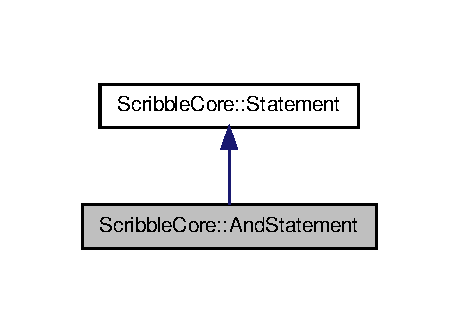
\includegraphics[width=226pt]{class_scribble_core_1_1_and_statement__inherit__graph}
\end{center}
\end{figure}


Collaboration diagram for Scribble\-Core\-:\-:And\-Statement\-:
\nopagebreak
\begin{figure}[H]
\begin{center}
\leavevmode
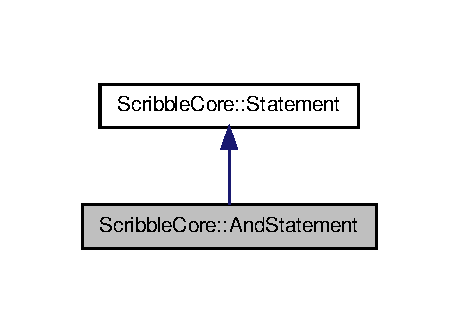
\includegraphics[width=226pt]{class_scribble_core_1_1_and_statement__coll__graph}
\end{center}
\end{figure}
\subsection*{Public Member Functions}
\begin{DoxyCompactItemize}
\item 
\hyperlink{class_scribble_core_1_1_and_statement_a46efe1fa7d7668c486ef12269f9e40bc}{And\-Statement} (int line\-No, std\-::string sym, \hyperlink{namespace_scribble_core_a2ad5bf236bc9164cb56f564685f15a11}{Safe\-Statement} left\-Hand\-Side, \hyperlink{namespace_scribble_core_a2ad5bf236bc9164cb56f564685f15a11}{Safe\-Statement} right\-Hand\-Side)
\item 
virtual \hyperlink{class_scribble_core_1_1_and_statement_a491c2d0fef506f2001a669d4b900c133}{$\sim$\-And\-Statement} ()
\item 
virtual void \hyperlink{class_scribble_core_1_1_and_statement_a1c5599274c07acc22593b5d46ce13067}{check\-Tree} (\hyperlink{class_scribble_core_1_1_type}{Type} $\ast$function\-Type)
\item 
virtual \hyperlink{class_scribble_core_1_1_type}{Type} $\ast$ \hyperlink{class_scribble_core_1_1_and_statement_a957b93b036c51ac746c18ad7fbfcda71}{type} ()
\item 
int \hyperlink{class_scribble_core_1_1_and_statement_a314da1cf611fd6ae02f126e12a80307d}{generate\-Code} (int result\-Register, std\-::stringstream \&generated)
\end{DoxyCompactItemize}


\subsection{Detailed Description}
The and statement returns true if the left and right hand expressions both evaluate to true.

If the left side is false then the right side will not be checked. 

Definition at line 21 of file And\-Statement.\-hpp.



\subsection{Constructor \& Destructor Documentation}
\hypertarget{class_scribble_core_1_1_and_statement_a46efe1fa7d7668c486ef12269f9e40bc}{\index{Scribble\-Core\-::\-And\-Statement@{Scribble\-Core\-::\-And\-Statement}!And\-Statement@{And\-Statement}}
\index{And\-Statement@{And\-Statement}!ScribbleCore::AndStatement@{Scribble\-Core\-::\-And\-Statement}}
\subsubsection[{And\-Statement}]{\setlength{\rightskip}{0pt plus 5cm}Scribble\-Core\-::\-And\-Statement\-::\-And\-Statement (
\begin{DoxyParamCaption}
\item[{int}]{line\-No, }
\item[{std\-::string}]{sym, }
\item[{{\bf Safe\-Statement}}]{left\-Hand\-Side, }
\item[{{\bf Safe\-Statement}}]{right\-Hand\-Side}
\end{DoxyParamCaption}
)}}\label{class_scribble_core_1_1_and_statement_a46efe1fa7d7668c486ef12269f9e40bc}


Definition at line 15 of file And\-Statement.\-cpp.

\hypertarget{class_scribble_core_1_1_and_statement_a491c2d0fef506f2001a669d4b900c133}{\index{Scribble\-Core\-::\-And\-Statement@{Scribble\-Core\-::\-And\-Statement}!$\sim$\-And\-Statement@{$\sim$\-And\-Statement}}
\index{$\sim$\-And\-Statement@{$\sim$\-And\-Statement}!ScribbleCore::AndStatement@{Scribble\-Core\-::\-And\-Statement}}
\subsubsection[{$\sim$\-And\-Statement}]{\setlength{\rightskip}{0pt plus 5cm}Scribble\-Core\-::\-And\-Statement\-::$\sim$\-And\-Statement (
\begin{DoxyParamCaption}
{}
\end{DoxyParamCaption}
)\hspace{0.3cm}{\ttfamily [virtual]}}}\label{class_scribble_core_1_1_and_statement_a491c2d0fef506f2001a669d4b900c133}


Definition at line 22 of file And\-Statement.\-cpp.



\subsection{Member Function Documentation}
\hypertarget{class_scribble_core_1_1_and_statement_a1c5599274c07acc22593b5d46ce13067}{\index{Scribble\-Core\-::\-And\-Statement@{Scribble\-Core\-::\-And\-Statement}!check\-Tree@{check\-Tree}}
\index{check\-Tree@{check\-Tree}!ScribbleCore::AndStatement@{Scribble\-Core\-::\-And\-Statement}}
\subsubsection[{check\-Tree}]{\setlength{\rightskip}{0pt plus 5cm}void Scribble\-Core\-::\-And\-Statement\-::check\-Tree (
\begin{DoxyParamCaption}
\item[{{\bf Type} $\ast$}]{function\-Type}
\end{DoxyParamCaption}
)\hspace{0.3cm}{\ttfamily [virtual]}}}\label{class_scribble_core_1_1_and_statement_a1c5599274c07acc22593b5d46ce13067}


Implements \hyperlink{class_scribble_core_1_1_statement_a894e4f8d8b35279bb9ea87f20afdb978}{Scribble\-Core\-::\-Statement}.



Definition at line 26 of file And\-Statement.\-cpp.



Here is the call graph for this function\-:
\nopagebreak
\begin{figure}[H]
\begin{center}
\leavevmode
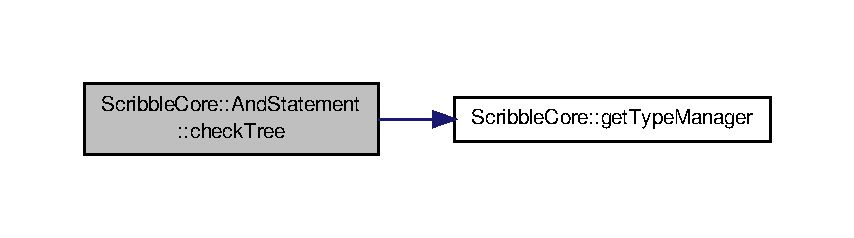
\includegraphics[width=350pt]{class_scribble_core_1_1_and_statement_a1c5599274c07acc22593b5d46ce13067_cgraph}
\end{center}
\end{figure}


\hypertarget{class_scribble_core_1_1_and_statement_a314da1cf611fd6ae02f126e12a80307d}{\index{Scribble\-Core\-::\-And\-Statement@{Scribble\-Core\-::\-And\-Statement}!generate\-Code@{generate\-Code}}
\index{generate\-Code@{generate\-Code}!ScribbleCore::AndStatement@{Scribble\-Core\-::\-And\-Statement}}
\subsubsection[{generate\-Code}]{\setlength{\rightskip}{0pt plus 5cm}int Scribble\-Core\-::\-And\-Statement\-::generate\-Code (
\begin{DoxyParamCaption}
\item[{int}]{result\-Register, }
\item[{std\-::stringstream \&}]{generated}
\end{DoxyParamCaption}
)\hspace{0.3cm}{\ttfamily [virtual]}}}\label{class_scribble_core_1_1_and_statement_a314da1cf611fd6ae02f126e12a80307d}


Reimplemented from \hyperlink{class_scribble_core_1_1_statement_aa3951ffef06ca195054a0bdfc8a4c8de}{Scribble\-Core\-::\-Statement}.



Definition at line 44 of file And\-Statement.\-cpp.

\hypertarget{class_scribble_core_1_1_and_statement_a957b93b036c51ac746c18ad7fbfcda71}{\index{Scribble\-Core\-::\-And\-Statement@{Scribble\-Core\-::\-And\-Statement}!type@{type}}
\index{type@{type}!ScribbleCore::AndStatement@{Scribble\-Core\-::\-And\-Statement}}
\subsubsection[{type}]{\setlength{\rightskip}{0pt plus 5cm}{\bf Type} $\ast$ Scribble\-Core\-::\-And\-Statement\-::type (
\begin{DoxyParamCaption}
{}
\end{DoxyParamCaption}
)\hspace{0.3cm}{\ttfamily [virtual]}}}\label{class_scribble_core_1_1_and_statement_a957b93b036c51ac746c18ad7fbfcda71}
And\-Statements type is boolean. 

Implements \hyperlink{class_scribble_core_1_1_statement_a532ed5a44ec49873dc191dae7ddc8b00}{Scribble\-Core\-::\-Statement}.



Definition at line 40 of file And\-Statement.\-cpp.



Here is the call graph for this function\-:
\nopagebreak
\begin{figure}[H]
\begin{center}
\leavevmode
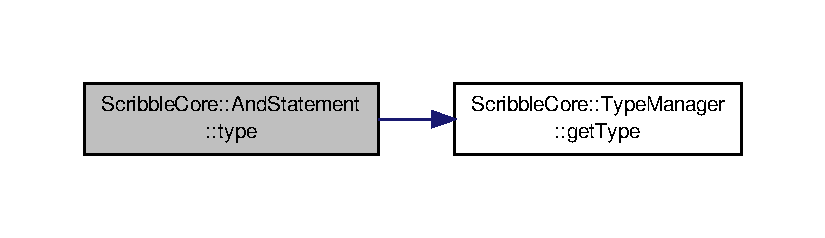
\includegraphics[width=350pt]{class_scribble_core_1_1_and_statement_a957b93b036c51ac746c18ad7fbfcda71_cgraph}
\end{center}
\end{figure}




The documentation for this class was generated from the following files\-:\begin{DoxyCompactItemize}
\item 
/home/blake/\-Dropbox/\-Current/\-Scribble/src/\-Scribble/\-Statement/\hyperlink{_and_statement_8hpp}{And\-Statement.\-hpp}\item 
/home/blake/\-Dropbox/\-Current/\-Scribble/src/\-Scribble/\-Statement/\hyperlink{_and_statement_8cpp}{And\-Statement.\-cpp}\end{DoxyCompactItemize}

\hypertarget{class_a_p_i_1_1_a_p_i_function}{\section{A\-P\-I\-:\-:A\-P\-I\-Function Class Reference}
\label{class_a_p_i_1_1_a_p_i_function}\index{A\-P\-I\-::\-A\-P\-I\-Function@{A\-P\-I\-::\-A\-P\-I\-Function}}
}


{\ttfamily \#include $<$A\-P\-I\-Function.\-hpp$>$}



Inheritance diagram for A\-P\-I\-:\-:A\-P\-I\-Function\-:
\nopagebreak
\begin{figure}[H]
\begin{center}
\leavevmode
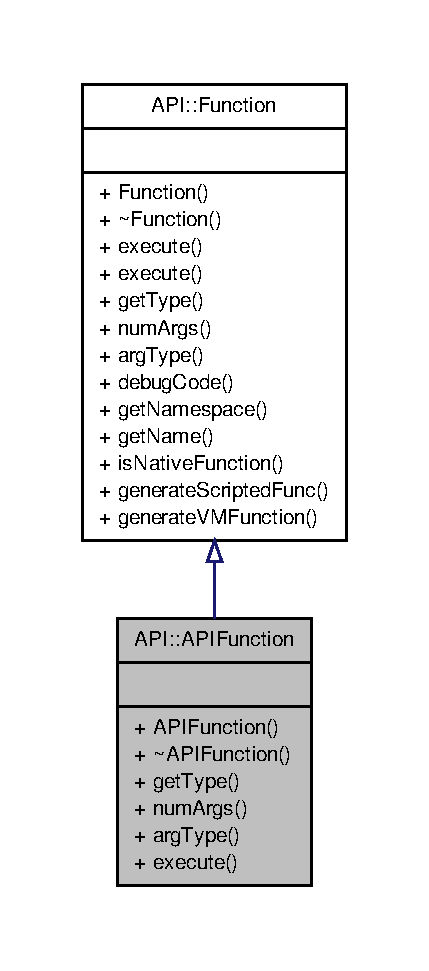
\includegraphics[width=206pt]{class_a_p_i_1_1_a_p_i_function__inherit__graph}
\end{center}
\end{figure}


Collaboration diagram for A\-P\-I\-:\-:A\-P\-I\-Function\-:
\nopagebreak
\begin{figure}[H]
\begin{center}
\leavevmode
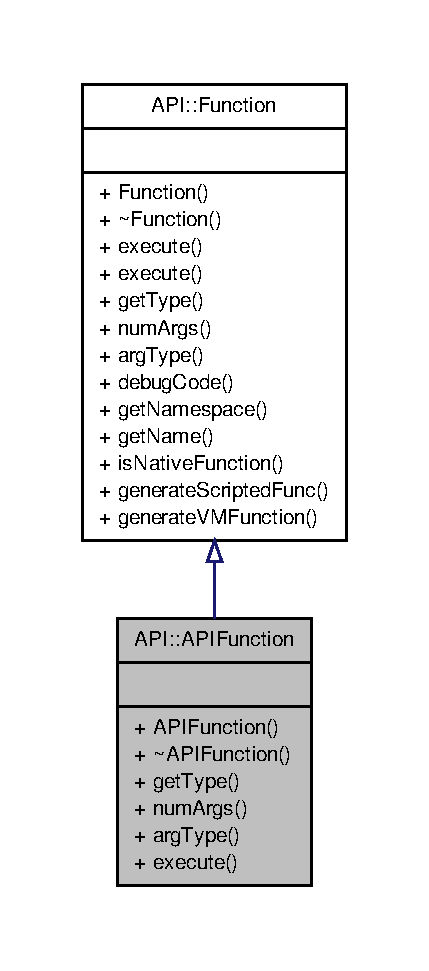
\includegraphics[width=206pt]{class_a_p_i_1_1_a_p_i_function__coll__graph}
\end{center}
\end{figure}
\subsection*{Public Member Functions}
\begin{DoxyCompactItemize}
\item 
\hyperlink{class_a_p_i_1_1_a_p_i_function_afea25b0659c827f353062798fb643e81}{A\-P\-I\-Function} (std\-::string name, std\-::string package, \hyperlink{class_scribble_core_1_1_type}{Scribble\-Core\-::\-Type} $\ast$return\-Type, std\-::vector$<$ \hyperlink{class_scribble_core_1_1_type}{Scribble\-Core\-::\-Type} $\ast$ $>$ types, \hyperlink{class_a_p_i_1_1_a_p_i_value}{A\-P\-I\-::\-A\-P\-I\-Value}($\ast$fn)(\hyperlink{class_a_p_i_1_1_a_p_i_value}{A\-P\-I\-::\-A\-P\-I\-Value} $\ast$, \hyperlink{class_v_m_1_1_virtual_machine}{V\-M\-::\-Virtual\-Machine} $\ast$virt))
\item 
virtual \hyperlink{class_a_p_i_1_1_a_p_i_function_a2dc447ed768ed299cd18b6f3226a2484}{$\sim$\-A\-P\-I\-Function} ()
\item 
\hyperlink{class_scribble_core_1_1_type}{Scribble\-Core\-::\-Type} $\ast$ \hyperlink{class_a_p_i_1_1_a_p_i_function_a7b3106c0510d471df41eb8e972205585}{get\-Type} ()
\item 
const unsigned int \hyperlink{class_a_p_i_1_1_a_p_i_function_a6544abd1ce33a241c71de9bad62547ab}{num\-Args} ()
\item 
\hyperlink{class_scribble_core_1_1_type}{Scribble\-Core\-::\-Type} $\ast$ \hyperlink{class_a_p_i_1_1_a_p_i_function_a086936a84a8c7b0490fee3f8c303435b}{arg\-Type} (unsigned int arg)
\item 
\hyperlink{class_a_p_i_1_1_a_p_i_value}{A\-P\-I\-Value} \hyperlink{class_a_p_i_1_1_a_p_i_function_a077954335c03ec3ebcc31aa746c9026a}{execute} (\hyperlink{class_a_p_i_1_1_a_p_i_value}{A\-P\-I\-::\-A\-P\-I\-Value} $\ast$values, \hyperlink{class_v_m_1_1_virtual_machine}{V\-M\-::\-Virtual\-Machine} $\ast$virt)
\end{DoxyCompactItemize}
\subsection*{Additional Inherited Members}


\subsection{Detailed Description}


Definition at line 17 of file A\-P\-I\-Function.\-hpp.



\subsection{Constructor \& Destructor Documentation}
\hypertarget{class_a_p_i_1_1_a_p_i_function_afea25b0659c827f353062798fb643e81}{\index{A\-P\-I\-::\-A\-P\-I\-Function@{A\-P\-I\-::\-A\-P\-I\-Function}!A\-P\-I\-Function@{A\-P\-I\-Function}}
\index{A\-P\-I\-Function@{A\-P\-I\-Function}!API::APIFunction@{A\-P\-I\-::\-A\-P\-I\-Function}}
\subsubsection[{A\-P\-I\-Function}]{\setlength{\rightskip}{0pt plus 5cm}A\-P\-I\-::\-A\-P\-I\-Function\-::\-A\-P\-I\-Function (
\begin{DoxyParamCaption}
\item[{std\-::string}]{name, }
\item[{std\-::string}]{package, }
\item[{{\bf Scribble\-Core\-::\-Type} $\ast$}]{return\-Type, }
\item[{std\-::vector$<$ {\bf Scribble\-Core\-::\-Type} $\ast$ $>$}]{types, }
\item[{{\bf A\-P\-I\-::\-A\-P\-I\-Value}($\ast$)({\bf A\-P\-I\-::\-A\-P\-I\-Value} $\ast$, {\bf V\-M\-::\-Virtual\-Machine} $\ast$virt)}]{fn}
\end{DoxyParamCaption}
)}}\label{class_a_p_i_1_1_a_p_i_function_afea25b0659c827f353062798fb643e81}


Definition at line 12 of file A\-P\-I\-Function.\-cpp.

\hypertarget{class_a_p_i_1_1_a_p_i_function_a2dc447ed768ed299cd18b6f3226a2484}{\index{A\-P\-I\-::\-A\-P\-I\-Function@{A\-P\-I\-::\-A\-P\-I\-Function}!$\sim$\-A\-P\-I\-Function@{$\sim$\-A\-P\-I\-Function}}
\index{$\sim$\-A\-P\-I\-Function@{$\sim$\-A\-P\-I\-Function}!API::APIFunction@{A\-P\-I\-::\-A\-P\-I\-Function}}
\subsubsection[{$\sim$\-A\-P\-I\-Function}]{\setlength{\rightskip}{0pt plus 5cm}A\-P\-I\-::\-A\-P\-I\-Function\-::$\sim$\-A\-P\-I\-Function (
\begin{DoxyParamCaption}
{}
\end{DoxyParamCaption}
)\hspace{0.3cm}{\ttfamily [virtual]}}}\label{class_a_p_i_1_1_a_p_i_function_a2dc447ed768ed299cd18b6f3226a2484}


Definition at line 17 of file A\-P\-I\-Function.\-cpp.



\subsection{Member Function Documentation}
\hypertarget{class_a_p_i_1_1_a_p_i_function_a086936a84a8c7b0490fee3f8c303435b}{\index{A\-P\-I\-::\-A\-P\-I\-Function@{A\-P\-I\-::\-A\-P\-I\-Function}!arg\-Type@{arg\-Type}}
\index{arg\-Type@{arg\-Type}!API::APIFunction@{A\-P\-I\-::\-A\-P\-I\-Function}}
\subsubsection[{arg\-Type}]{\setlength{\rightskip}{0pt plus 5cm}{\bf Scribble\-Core\-::\-Type}$\ast$ A\-P\-I\-::\-A\-P\-I\-Function\-::arg\-Type (
\begin{DoxyParamCaption}
\item[{unsigned int}]{arg}
\end{DoxyParamCaption}
)\hspace{0.3cm}{\ttfamily [inline]}, {\ttfamily [virtual]}}}\label{class_a_p_i_1_1_a_p_i_function_a086936a84a8c7b0490fee3f8c303435b}
Get the expected type of the specified argument 

Implements \hyperlink{class_a_p_i_1_1_function_a531806ea8476e8aa396eb98ce81e713b}{A\-P\-I\-::\-Function}.



Definition at line 38 of file A\-P\-I\-Function.\-hpp.

\hypertarget{class_a_p_i_1_1_a_p_i_function_a077954335c03ec3ebcc31aa746c9026a}{\index{A\-P\-I\-::\-A\-P\-I\-Function@{A\-P\-I\-::\-A\-P\-I\-Function}!execute@{execute}}
\index{execute@{execute}!API::APIFunction@{A\-P\-I\-::\-A\-P\-I\-Function}}
\subsubsection[{execute}]{\setlength{\rightskip}{0pt plus 5cm}{\bf A\-P\-I\-Value} A\-P\-I\-::\-A\-P\-I\-Function\-::execute (
\begin{DoxyParamCaption}
\item[{{\bf A\-P\-I\-::\-A\-P\-I\-Value} $\ast$}]{values, }
\item[{{\bf V\-M\-::\-Virtual\-Machine} $\ast$}]{virt}
\end{DoxyParamCaption}
)\hspace{0.3cm}{\ttfamily [inline]}, {\ttfamily [virtual]}}}\label{class_a_p_i_1_1_a_p_i_function_a077954335c03ec3ebcc31aa746c9026a}
This function executes the given \hyperlink{class_a_p_i_1_1_function}{A\-P\-I\-::\-Function} and returns it's result. It called by the more complex \hyperlink{class_a_p_i_1_1_function_a5acc2022cdbd5fe47c1a04769a1d8cf4}{execute(\-V\-M\-::\-Virtual\-Machine$\ast$)} after that function has converted all arguments into \hyperlink{namespace_a_p_i}{A\-P\-I} values. 
\begin{DoxyParams}{Parameters}
{\em args} & The arguments passed to the function \\
\hline
{\em virt} & The virtual machine this function is being run in the context of. \\
\hline
\end{DoxyParams}
\begin{DoxyReturn}{Returns}
The resulting \hyperlink{namespace_a_p_i}{A\-P\-I} value 
\end{DoxyReturn}


Reimplemented from \hyperlink{class_a_p_i_1_1_function_ac3bc5de6ce095a4c8474525ef181c4af}{A\-P\-I\-::\-Function}.



Definition at line 42 of file A\-P\-I\-Function.\-hpp.

\hypertarget{class_a_p_i_1_1_a_p_i_function_a7b3106c0510d471df41eb8e972205585}{\index{A\-P\-I\-::\-A\-P\-I\-Function@{A\-P\-I\-::\-A\-P\-I\-Function}!get\-Type@{get\-Type}}
\index{get\-Type@{get\-Type}!API::APIFunction@{A\-P\-I\-::\-A\-P\-I\-Function}}
\subsubsection[{get\-Type}]{\setlength{\rightskip}{0pt plus 5cm}{\bf Scribble\-Core\-::\-Type}$\ast$ A\-P\-I\-::\-A\-P\-I\-Function\-::get\-Type (
\begin{DoxyParamCaption}
{}
\end{DoxyParamCaption}
)\hspace{0.3cm}{\ttfamily [inline]}, {\ttfamily [virtual]}}}\label{class_a_p_i_1_1_a_p_i_function_a7b3106c0510d471df41eb8e972205585}
Get the return type of the function 

Implements \hyperlink{class_a_p_i_1_1_function_a85b0b2ee88d3ac61a0e77f94e06445b1}{A\-P\-I\-::\-Function}.



Definition at line 30 of file A\-P\-I\-Function.\-hpp.

\hypertarget{class_a_p_i_1_1_a_p_i_function_a6544abd1ce33a241c71de9bad62547ab}{\index{A\-P\-I\-::\-A\-P\-I\-Function@{A\-P\-I\-::\-A\-P\-I\-Function}!num\-Args@{num\-Args}}
\index{num\-Args@{num\-Args}!API::APIFunction@{A\-P\-I\-::\-A\-P\-I\-Function}}
\subsubsection[{num\-Args}]{\setlength{\rightskip}{0pt plus 5cm}const unsigned int A\-P\-I\-::\-A\-P\-I\-Function\-::num\-Args (
\begin{DoxyParamCaption}
{}
\end{DoxyParamCaption}
)\hspace{0.3cm}{\ttfamily [inline]}, {\ttfamily [virtual]}}}\label{class_a_p_i_1_1_a_p_i_function_a6544abd1ce33a241c71de9bad62547ab}
Return the number of arguments the function takes 

Implements \hyperlink{class_a_p_i_1_1_function_ae56761ad4c849c05e12cb4cd02583c77}{A\-P\-I\-::\-Function}.



Definition at line 34 of file A\-P\-I\-Function.\-hpp.



The documentation for this class was generated from the following files\-:\begin{DoxyCompactItemize}
\item 
/home/blake/\-Dropbox/\-Current/\-Scribble/src/\-A\-P\-I/\hyperlink{_a_p_i_function_8hpp}{A\-P\-I\-Function.\-hpp}\item 
/home/blake/\-Dropbox/\-Current/\-Scribble/src/\-A\-P\-I/\hyperlink{_a_p_i_function_8cpp}{A\-P\-I\-Function.\-cpp}\end{DoxyCompactItemize}

\hypertarget{class_a_p_i_1_1_a_p_i_value}{\section{A\-P\-I\-:\-:A\-P\-I\-Value Class Reference}
\label{class_a_p_i_1_1_a_p_i_value}\index{A\-P\-I\-::\-A\-P\-I\-Value@{A\-P\-I\-::\-A\-P\-I\-Value}}
}


{\ttfamily \#include $<$A\-P\-I\-Value.\-hpp$>$}



Collaboration diagram for A\-P\-I\-:\-:A\-P\-I\-Value\-:
\nopagebreak
\begin{figure}[H]
\begin{center}
\leavevmode
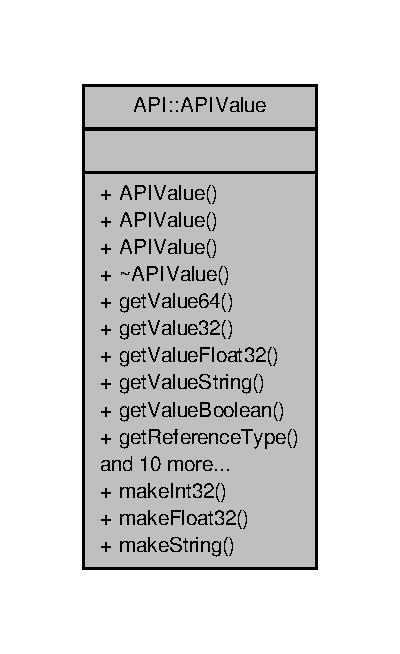
\includegraphics[width=192pt]{class_a_p_i_1_1_a_p_i_value__coll__graph}
\end{center}
\end{figure}
\subsection*{Public Member Functions}
\begin{DoxyCompactItemize}
\item 
\hyperlink{class_a_p_i_1_1_a_p_i_value_ac687584e4a3f04eded7a7b2e178331ae}{A\-P\-I\-Value} ()
\item 
\hyperlink{class_a_p_i_1_1_a_p_i_value_aa9c18784d818a39bf8ff1f91a5a9fa44}{A\-P\-I\-Value} (\hyperlink{class_scribble_core_1_1_type}{Scribble\-Core\-::\-Type} $\ast$type, int64\-\_\-t val)
\item 
\hyperlink{class_a_p_i_1_1_a_p_i_value_ac6a9936ffcc934fd6e16fa9d26d2732c}{A\-P\-I\-Value} (\hyperlink{class_scribble_core_1_1_type}{Scribble\-Core\-::\-Type} $\ast$type, \hyperlink{_smart_pointer_8hpp_afdd8d4ba81c3fcbdeacf1dafba2accfb}{Smart\-Pointer}$<$ \hyperlink{class_v_m_1_1_v_m_entry_type}{V\-M\-::\-V\-M\-Entry\-Type} $>$ vm\-Type, \hyperlink{_smart_pointer_8hpp_afdd8d4ba81c3fcbdeacf1dafba2accfb}{Smart\-Pointer}$<$ uint8\-\_\-t $>$ data, long val)
\item 
virtual \hyperlink{class_a_p_i_1_1_a_p_i_value_a3a23f788748db18999b767932abb0672}{$\sim$\-A\-P\-I\-Value} ()
\item 
int64\-\_\-t \hyperlink{class_a_p_i_1_1_a_p_i_value_a26380a603f4fc9191608f047e6ea8250}{get\-Value64} ()
\item 
int32\-\_\-t \hyperlink{class_a_p_i_1_1_a_p_i_value_ae56a74e043a259b1a219804cb77165d7}{get\-Value32} ()
\item 
\hyperlink{types_8h_a4611b605e45ab401f02cab15c5e38715}{float32\-\_\-t} \hyperlink{class_a_p_i_1_1_a_p_i_value_a2374ba437041f0c57514be649825312b}{get\-Value\-Float32} ()
\item 
char $\ast$ \hyperlink{class_a_p_i_1_1_a_p_i_value_a94eb3d9f4b1c0dfd397f6813fd8c8a94}{get\-Value\-String} ()
\item 
bool \hyperlink{class_a_p_i_1_1_a_p_i_value_a720e381988acbc87b34df8535d61e4d2}{get\-Value\-Boolean} ()
\item 
\hyperlink{_smart_pointer_8hpp_afdd8d4ba81c3fcbdeacf1dafba2accfb}{Smart\-Pointer}$<$ \hyperlink{class_v_m_1_1_v_m_entry_type}{V\-M\-::\-V\-M\-Entry\-Type} $>$ \hyperlink{class_a_p_i_1_1_a_p_i_value_adffeaebde4496d5ee7e9944f1aa4bb76}{get\-Reference\-Type} ()
\item 
uint8\-\_\-t $\ast$ \hyperlink{class_a_p_i_1_1_a_p_i_value_afaee05a374fbc7e04c9ceb9f4b0758af}{get\-Reference\-Pointer} ()
\item 
\hyperlink{class_scribble_core_1_1_type}{Scribble\-Core\-::\-Type} $\ast$ \hyperlink{class_a_p_i_1_1_a_p_i_value_a50687d887d23aabffd1f9df7f3ba94a1}{get\-Type} ()
\item 
bool \hyperlink{class_a_p_i_1_1_a_p_i_value_a9f5b34b9c70f6279dea8f556698ca1f6}{is\-Reference} ()
\item 
bool \hyperlink{class_a_p_i_1_1_a_p_i_value_a8a97634f469ced8407f4ca6cdd0f9898}{is\-Null} ()
\item 
\hyperlink{class_a_p_i_1_1_a_p_i_value}{A\-P\-I\-Value} \hyperlink{class_a_p_i_1_1_a_p_i_value_ac52ce1c55cc0a808016b557d1fb74995}{get\-Field} (std\-::string const \&name, \hyperlink{class_v_m_1_1_virtual_machine}{V\-M\-::\-Virtual\-Machine} $\ast$vm)
\item 
unsigned int \hyperlink{class_a_p_i_1_1_a_p_i_value_a1506f360a478ac864b76fec0409bc117}{get\-Array\-Length} (\hyperlink{class_v_m_1_1_virtual_machine}{V\-M\-::\-Virtual\-Machine} $\ast$vm)
\item 
\hyperlink{class_a_p_i_1_1_a_p_i_value}{A\-P\-I\-Value} \hyperlink{class_a_p_i_1_1_a_p_i_value_a799ace497f1988f95af61d6796d67a19}{get\-Index} (unsigned int index, \hyperlink{class_v_m_1_1_virtual_machine}{V\-M\-::\-Virtual\-Machine} $\ast$vm)
\item 
void \hyperlink{class_a_p_i_1_1_a_p_i_value_aa516e6d20f842e2dfd60c1c59a697312}{set\-Field} (std\-::string const \&name, \hyperlink{class_a_p_i_1_1_a_p_i_value}{A\-P\-I\-::\-A\-P\-I\-Value} val, \hyperlink{class_v_m_1_1_virtual_machine}{V\-M\-::\-Virtual\-Machine} $\ast$vm)
\item 
void \hyperlink{class_a_p_i_1_1_a_p_i_value_aa8a379bf602fc10523bfc4a4867dbc55}{set\-Index} (unsigned int index, \hyperlink{class_a_p_i_1_1_a_p_i_value}{A\-P\-I\-::\-A\-P\-I\-Value} val, \hyperlink{class_v_m_1_1_virtual_machine}{V\-M\-::\-Virtual\-Machine} $\ast$vm)
\item 
void \hyperlink{class_a_p_i_1_1_a_p_i_value_a54a170b1214ed9daf309c889b7daf77e}{push\-To\-V\-M} (\hyperlink{class_v_m_1_1_virtual_machine}{V\-M\-::\-Virtual\-Machine} $\ast$virt)
\end{DoxyCompactItemize}
\subsection*{Static Public Member Functions}
\begin{DoxyCompactItemize}
\item 
static \hyperlink{class_a_p_i_1_1_a_p_i_value}{A\-P\-I\-::\-A\-P\-I\-Value} \hyperlink{class_a_p_i_1_1_a_p_i_value_a5d2ee6a2550a35698b7f63678c64fc47}{make\-Int32} (int val)
\item 
static \hyperlink{class_a_p_i_1_1_a_p_i_value}{A\-P\-I\-::\-A\-P\-I\-Value} \hyperlink{class_a_p_i_1_1_a_p_i_value_ae4d8ca7c8a72f24e3b7419cc4fc2127c}{make\-Float32} (\hyperlink{types_8h_a4611b605e45ab401f02cab15c5e38715}{float32\-\_\-t} val)
\item 
static \hyperlink{class_a_p_i_1_1_a_p_i_value}{A\-P\-I\-::\-A\-P\-I\-Value} \hyperlink{class_a_p_i_1_1_a_p_i_value_abc6491d068cfc443ef5cbbc83156e46e}{make\-String} (std\-::string const \&text, \hyperlink{class_v_m_1_1_virtual_machine}{V\-M\-::\-Virtual\-Machine} $\ast$vm)
\end{DoxyCompactItemize}


\subsection{Detailed Description}
The \hyperlink{class_a_p_i_1_1_a_p_i_value}{A\-P\-I\-Value} class contains the arguments for or return value from a virtual machine function.

It is a wrapper around the register value and heap data to provide an easy way to extra useful data from the result of a \hyperlink{namespace_v_m}{V\-M} execution or pass information to it. 

Definition at line 39 of file A\-P\-I\-Value.\-hpp.



\subsection{Constructor \& Destructor Documentation}
\hypertarget{class_a_p_i_1_1_a_p_i_value_ac687584e4a3f04eded7a7b2e178331ae}{\index{A\-P\-I\-::\-A\-P\-I\-Value@{A\-P\-I\-::\-A\-P\-I\-Value}!A\-P\-I\-Value@{A\-P\-I\-Value}}
\index{A\-P\-I\-Value@{A\-P\-I\-Value}!API::APIValue@{A\-P\-I\-::\-A\-P\-I\-Value}}
\subsubsection[{A\-P\-I\-Value}]{\setlength{\rightskip}{0pt plus 5cm}A\-P\-I\-::\-A\-P\-I\-Value\-::\-A\-P\-I\-Value (
\begin{DoxyParamCaption}
{}
\end{DoxyParamCaption}
)\hspace{0.3cm}{\ttfamily [inline]}}}\label{class_a_p_i_1_1_a_p_i_value_ac687584e4a3f04eded7a7b2e178331ae}


Definition at line 47 of file A\-P\-I\-Value.\-hpp.



Here is the call graph for this function\-:
\nopagebreak
\begin{figure}[H]
\begin{center}
\leavevmode
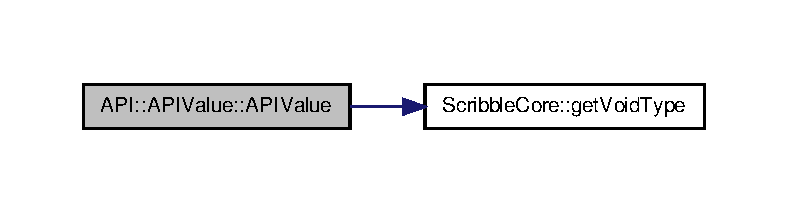
\includegraphics[width=350pt]{class_a_p_i_1_1_a_p_i_value_ac687584e4a3f04eded7a7b2e178331ae_cgraph}
\end{center}
\end{figure}




Here is the caller graph for this function\-:
\nopagebreak
\begin{figure}[H]
\begin{center}
\leavevmode
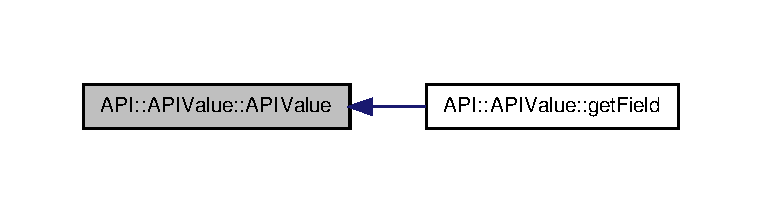
\includegraphics[width=350pt]{class_a_p_i_1_1_a_p_i_value_ac687584e4a3f04eded7a7b2e178331ae_icgraph}
\end{center}
\end{figure}


\hypertarget{class_a_p_i_1_1_a_p_i_value_aa9c18784d818a39bf8ff1f91a5a9fa44}{\index{A\-P\-I\-::\-A\-P\-I\-Value@{A\-P\-I\-::\-A\-P\-I\-Value}!A\-P\-I\-Value@{A\-P\-I\-Value}}
\index{A\-P\-I\-Value@{A\-P\-I\-Value}!API::APIValue@{A\-P\-I\-::\-A\-P\-I\-Value}}
\subsubsection[{A\-P\-I\-Value}]{\setlength{\rightskip}{0pt plus 5cm}A\-P\-I\-::\-A\-P\-I\-Value\-::\-A\-P\-I\-Value (
\begin{DoxyParamCaption}
\item[{{\bf Scribble\-Core\-::\-Type} $\ast$}]{type, }
\item[{int64\-\_\-t}]{val}
\end{DoxyParamCaption}
)}}\label{class_a_p_i_1_1_a_p_i_value_aa9c18784d818a39bf8ff1f91a5a9fa44}


Definition at line 12 of file A\-P\-I\-Value.\-cpp.

\hypertarget{class_a_p_i_1_1_a_p_i_value_ac6a9936ffcc934fd6e16fa9d26d2732c}{\index{A\-P\-I\-::\-A\-P\-I\-Value@{A\-P\-I\-::\-A\-P\-I\-Value}!A\-P\-I\-Value@{A\-P\-I\-Value}}
\index{A\-P\-I\-Value@{A\-P\-I\-Value}!API::APIValue@{A\-P\-I\-::\-A\-P\-I\-Value}}
\subsubsection[{A\-P\-I\-Value}]{\setlength{\rightskip}{0pt plus 5cm}A\-P\-I\-::\-A\-P\-I\-Value\-::\-A\-P\-I\-Value (
\begin{DoxyParamCaption}
\item[{{\bf Scribble\-Core\-::\-Type} $\ast$}]{type, }
\item[{{\bf Smart\-Pointer}$<$ {\bf V\-M\-::\-V\-M\-Entry\-Type} $>$}]{vm\-Type, }
\item[{{\bf Smart\-Pointer}$<$ uint8\-\_\-t $>$}]{data, }
\item[{long}]{val}
\end{DoxyParamCaption}
)}}\label{class_a_p_i_1_1_a_p_i_value_ac6a9936ffcc934fd6e16fa9d26d2732c}


Definition at line 16 of file A\-P\-I\-Value.\-cpp.

\hypertarget{class_a_p_i_1_1_a_p_i_value_a3a23f788748db18999b767932abb0672}{\index{A\-P\-I\-::\-A\-P\-I\-Value@{A\-P\-I\-::\-A\-P\-I\-Value}!$\sim$\-A\-P\-I\-Value@{$\sim$\-A\-P\-I\-Value}}
\index{$\sim$\-A\-P\-I\-Value@{$\sim$\-A\-P\-I\-Value}!API::APIValue@{A\-P\-I\-::\-A\-P\-I\-Value}}
\subsubsection[{$\sim$\-A\-P\-I\-Value}]{\setlength{\rightskip}{0pt plus 5cm}A\-P\-I\-::\-A\-P\-I\-Value\-::$\sim$\-A\-P\-I\-Value (
\begin{DoxyParamCaption}
{}
\end{DoxyParamCaption}
)\hspace{0.3cm}{\ttfamily [virtual]}}}\label{class_a_p_i_1_1_a_p_i_value_a3a23f788748db18999b767932abb0672}


Definition at line 21 of file A\-P\-I\-Value.\-cpp.



\subsection{Member Function Documentation}
\hypertarget{class_a_p_i_1_1_a_p_i_value_a1506f360a478ac864b76fec0409bc117}{\index{A\-P\-I\-::\-A\-P\-I\-Value@{A\-P\-I\-::\-A\-P\-I\-Value}!get\-Array\-Length@{get\-Array\-Length}}
\index{get\-Array\-Length@{get\-Array\-Length}!API::APIValue@{A\-P\-I\-::\-A\-P\-I\-Value}}
\subsubsection[{get\-Array\-Length}]{\setlength{\rightskip}{0pt plus 5cm}unsigned int A\-P\-I\-::\-A\-P\-I\-Value\-::get\-Array\-Length (
\begin{DoxyParamCaption}
\item[{{\bf V\-M\-::\-Virtual\-Machine} $\ast$}]{vm}
\end{DoxyParamCaption}
)\hspace{0.3cm}{\ttfamily [inline]}}}\label{class_a_p_i_1_1_a_p_i_value_a1506f360a478ac864b76fec0409bc117}
Return the length of the array pointer to by a reference.

If the A\-P\-Ivalue is not an array reference or the reference is a null reference then 0 will be returned. 

Definition at line 204 of file A\-P\-I\-Value.\-hpp.



Here is the call graph for this function\-:
\nopagebreak
\begin{figure}[H]
\begin{center}
\leavevmode
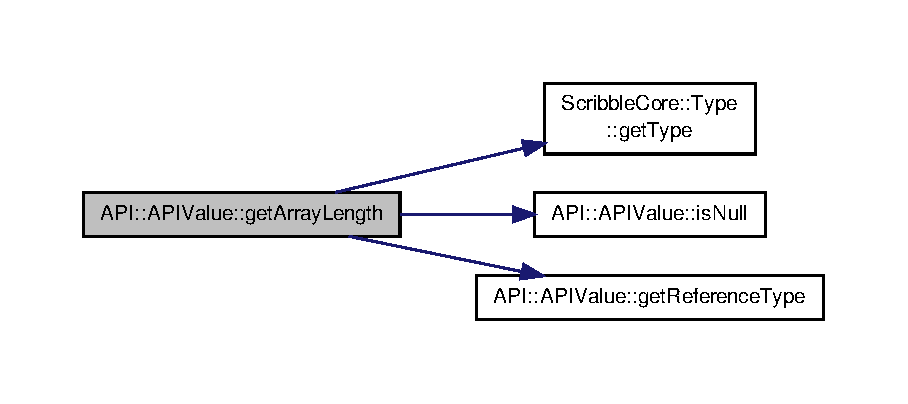
\includegraphics[width=350pt]{class_a_p_i_1_1_a_p_i_value_a1506f360a478ac864b76fec0409bc117_cgraph}
\end{center}
\end{figure}




Here is the caller graph for this function\-:
\nopagebreak
\begin{figure}[H]
\begin{center}
\leavevmode
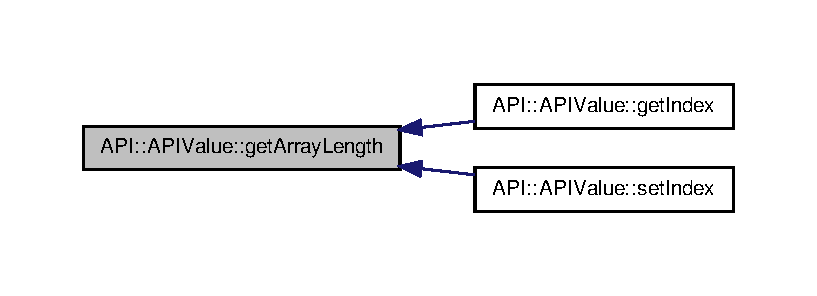
\includegraphics[width=350pt]{class_a_p_i_1_1_a_p_i_value_a1506f360a478ac864b76fec0409bc117_icgraph}
\end{center}
\end{figure}


\hypertarget{class_a_p_i_1_1_a_p_i_value_ac52ce1c55cc0a808016b557d1fb74995}{\index{A\-P\-I\-::\-A\-P\-I\-Value@{A\-P\-I\-::\-A\-P\-I\-Value}!get\-Field@{get\-Field}}
\index{get\-Field@{get\-Field}!API::APIValue@{A\-P\-I\-::\-A\-P\-I\-Value}}
\subsubsection[{get\-Field}]{\setlength{\rightskip}{0pt plus 5cm}{\bf A\-P\-I\-Value} A\-P\-I\-::\-A\-P\-I\-Value\-::get\-Field (
\begin{DoxyParamCaption}
\item[{std\-::string const \&}]{name, }
\item[{{\bf V\-M\-::\-Virtual\-Machine} $\ast$}]{vm}
\end{DoxyParamCaption}
)\hspace{0.3cm}{\ttfamily [inline]}}}\label{class_a_p_i_1_1_a_p_i_value_ac52ce1c55cc0a808016b557d1fb74995}
Will return the value of a field within the structure pointer to by a reference if that field exists. If the reference is not a structure or the field does not exist then A\-P\-I\-Value(0) will be returned. 

Definition at line 149 of file A\-P\-I\-Value.\-hpp.



Here is the call graph for this function\-:
\nopagebreak
\begin{figure}[H]
\begin{center}
\leavevmode
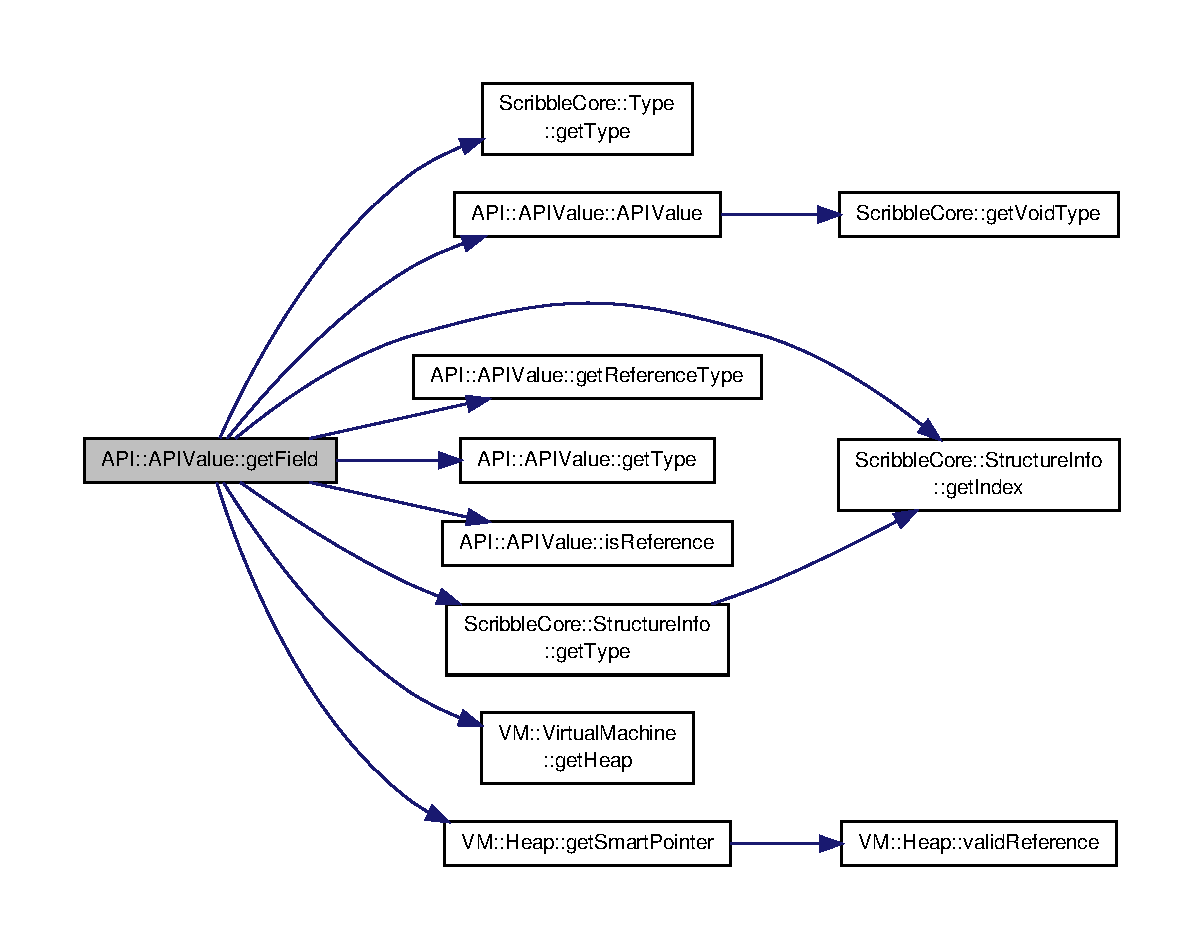
\includegraphics[width=350pt]{class_a_p_i_1_1_a_p_i_value_ac52ce1c55cc0a808016b557d1fb74995_cgraph}
\end{center}
\end{figure}


\hypertarget{class_a_p_i_1_1_a_p_i_value_a799ace497f1988f95af61d6796d67a19}{\index{A\-P\-I\-::\-A\-P\-I\-Value@{A\-P\-I\-::\-A\-P\-I\-Value}!get\-Index@{get\-Index}}
\index{get\-Index@{get\-Index}!API::APIValue@{A\-P\-I\-::\-A\-P\-I\-Value}}
\subsubsection[{get\-Index}]{\setlength{\rightskip}{0pt plus 5cm}{\bf A\-P\-I\-Value} A\-P\-I\-::\-A\-P\-I\-Value\-::get\-Index (
\begin{DoxyParamCaption}
\item[{unsigned int}]{index, }
\item[{{\bf V\-M\-::\-Virtual\-Machine} $\ast$}]{vm}
\end{DoxyParamCaption}
)\hspace{0.3cm}{\ttfamily [inline]}}}\label{class_a_p_i_1_1_a_p_i_value_a799ace497f1988f95af61d6796d67a19}


Definition at line 217 of file A\-P\-I\-Value.\-hpp.



Here is the call graph for this function\-:
\nopagebreak
\begin{figure}[H]
\begin{center}
\leavevmode
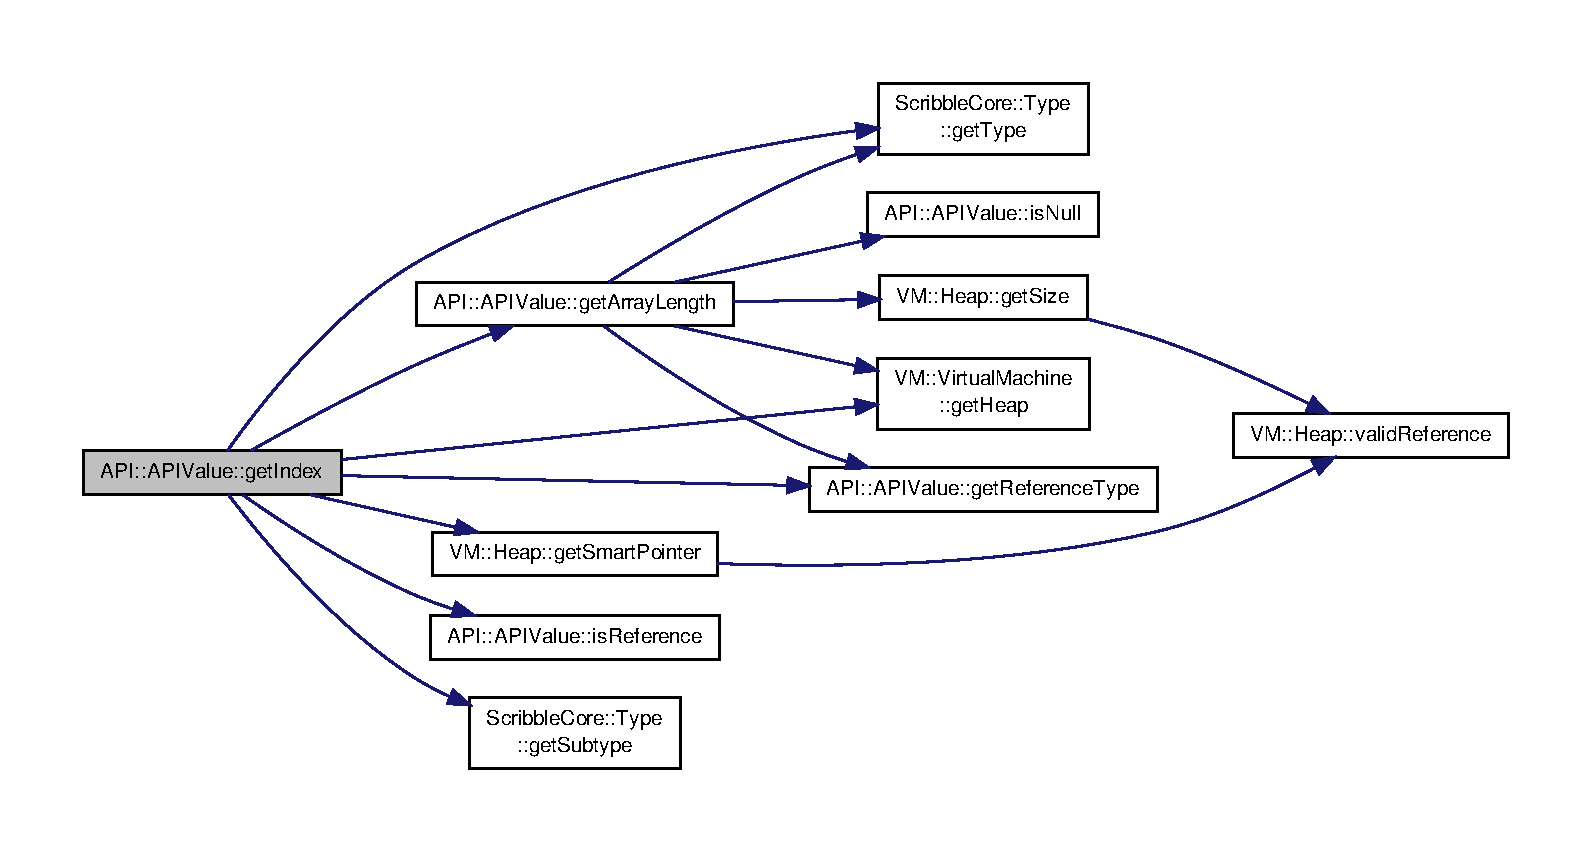
\includegraphics[width=350pt]{class_a_p_i_1_1_a_p_i_value_a799ace497f1988f95af61d6796d67a19_cgraph}
\end{center}
\end{figure}


\hypertarget{class_a_p_i_1_1_a_p_i_value_afaee05a374fbc7e04c9ceb9f4b0758af}{\index{A\-P\-I\-::\-A\-P\-I\-Value@{A\-P\-I\-::\-A\-P\-I\-Value}!get\-Reference\-Pointer@{get\-Reference\-Pointer}}
\index{get\-Reference\-Pointer@{get\-Reference\-Pointer}!API::APIValue@{A\-P\-I\-::\-A\-P\-I\-Value}}
\subsubsection[{get\-Reference\-Pointer}]{\setlength{\rightskip}{0pt plus 5cm}uint8\-\_\-t$\ast$ A\-P\-I\-::\-A\-P\-I\-Value\-::get\-Reference\-Pointer (
\begin{DoxyParamCaption}
{}
\end{DoxyParamCaption}
)\hspace{0.3cm}{\ttfamily [inline]}}}\label{class_a_p_i_1_1_a_p_i_value_afaee05a374fbc7e04c9ceb9f4b0758af}
For a reference this will return a pointer to the reference data, for primitive types this will return a null pointer. 

Definition at line 109 of file A\-P\-I\-Value.\-hpp.



Here is the caller graph for this function\-:
\nopagebreak
\begin{figure}[H]
\begin{center}
\leavevmode
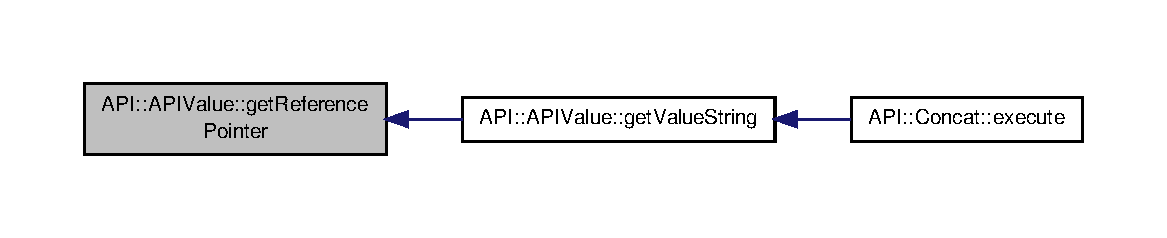
\includegraphics[width=350pt]{class_a_p_i_1_1_a_p_i_value_afaee05a374fbc7e04c9ceb9f4b0758af_icgraph}
\end{center}
\end{figure}


\hypertarget{class_a_p_i_1_1_a_p_i_value_adffeaebde4496d5ee7e9944f1aa4bb76}{\index{A\-P\-I\-::\-A\-P\-I\-Value@{A\-P\-I\-::\-A\-P\-I\-Value}!get\-Reference\-Type@{get\-Reference\-Type}}
\index{get\-Reference\-Type@{get\-Reference\-Type}!API::APIValue@{A\-P\-I\-::\-A\-P\-I\-Value}}
\subsubsection[{get\-Reference\-Type}]{\setlength{\rightskip}{0pt plus 5cm}{\bf Smart\-Pointer}$<${\bf V\-M\-::\-V\-M\-Entry\-Type}$>$ A\-P\-I\-::\-A\-P\-I\-Value\-::get\-Reference\-Type (
\begin{DoxyParamCaption}
{}
\end{DoxyParamCaption}
)\hspace{0.3cm}{\ttfamily [inline]}}}\label{class_a_p_i_1_1_a_p_i_value_adffeaebde4496d5ee7e9944f1aa4bb76}
If the value is a reference then return its type. 

Definition at line 101 of file A\-P\-I\-Value.\-hpp.



Here is the caller graph for this function\-:
\nopagebreak
\begin{figure}[H]
\begin{center}
\leavevmode
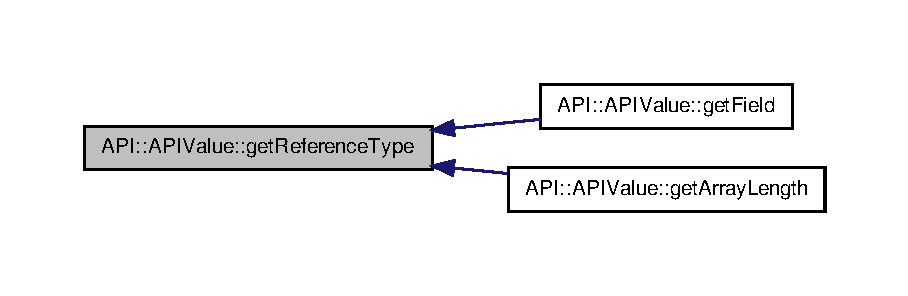
\includegraphics[width=350pt]{class_a_p_i_1_1_a_p_i_value_adffeaebde4496d5ee7e9944f1aa4bb76_icgraph}
\end{center}
\end{figure}


\hypertarget{class_a_p_i_1_1_a_p_i_value_a50687d887d23aabffd1f9df7f3ba94a1}{\index{A\-P\-I\-::\-A\-P\-I\-Value@{A\-P\-I\-::\-A\-P\-I\-Value}!get\-Type@{get\-Type}}
\index{get\-Type@{get\-Type}!API::APIValue@{A\-P\-I\-::\-A\-P\-I\-Value}}
\subsubsection[{get\-Type}]{\setlength{\rightskip}{0pt plus 5cm}{\bf Scribble\-Core\-::\-Type}$\ast$ A\-P\-I\-::\-A\-P\-I\-Value\-::get\-Type (
\begin{DoxyParamCaption}
{}
\end{DoxyParamCaption}
)\hspace{0.3cm}{\ttfamily [inline]}}}\label{class_a_p_i_1_1_a_p_i_value_a50687d887d23aabffd1f9df7f3ba94a1}


Definition at line 113 of file A\-P\-I\-Value.\-hpp.



Here is the caller graph for this function\-:
\nopagebreak
\begin{figure}[H]
\begin{center}
\leavevmode
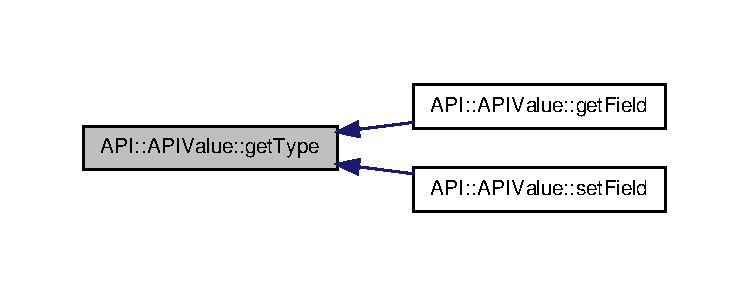
\includegraphics[width=350pt]{class_a_p_i_1_1_a_p_i_value_a50687d887d23aabffd1f9df7f3ba94a1_icgraph}
\end{center}
\end{figure}


\hypertarget{class_a_p_i_1_1_a_p_i_value_ae56a74e043a259b1a219804cb77165d7}{\index{A\-P\-I\-::\-A\-P\-I\-Value@{A\-P\-I\-::\-A\-P\-I\-Value}!get\-Value32@{get\-Value32}}
\index{get\-Value32@{get\-Value32}!API::APIValue@{A\-P\-I\-::\-A\-P\-I\-Value}}
\subsubsection[{get\-Value32}]{\setlength{\rightskip}{0pt plus 5cm}int32\-\_\-t A\-P\-I\-::\-A\-P\-I\-Value\-::get\-Value32 (
\begin{DoxyParamCaption}
{}
\end{DoxyParamCaption}
)\hspace{0.3cm}{\ttfamily [inline]}}}\label{class_a_p_i_1_1_a_p_i_value_ae56a74e043a259b1a219804cb77165d7}
This returns the value as a 32 bit signed integer. 

Definition at line 64 of file A\-P\-I\-Value.\-hpp.



Here is the caller graph for this function\-:
\nopagebreak
\begin{figure}[H]
\begin{center}
\leavevmode
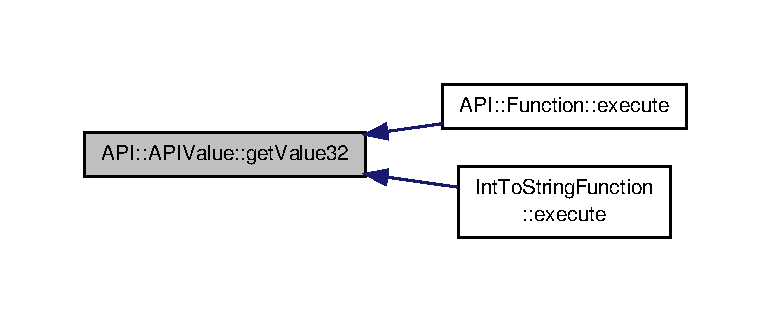
\includegraphics[width=350pt]{class_a_p_i_1_1_a_p_i_value_ae56a74e043a259b1a219804cb77165d7_icgraph}
\end{center}
\end{figure}


\hypertarget{class_a_p_i_1_1_a_p_i_value_a26380a603f4fc9191608f047e6ea8250}{\index{A\-P\-I\-::\-A\-P\-I\-Value@{A\-P\-I\-::\-A\-P\-I\-Value}!get\-Value64@{get\-Value64}}
\index{get\-Value64@{get\-Value64}!API::APIValue@{A\-P\-I\-::\-A\-P\-I\-Value}}
\subsubsection[{get\-Value64}]{\setlength{\rightskip}{0pt plus 5cm}int64\-\_\-t A\-P\-I\-::\-A\-P\-I\-Value\-::get\-Value64 (
\begin{DoxyParamCaption}
{}
\end{DoxyParamCaption}
)\hspace{0.3cm}{\ttfamily [inline]}}}\label{class_a_p_i_1_1_a_p_i_value_a26380a603f4fc9191608f047e6ea8250}
This returns the value as a 64 bit signed integer. 

Definition at line 56 of file A\-P\-I\-Value.\-hpp.



Here is the caller graph for this function\-:
\nopagebreak
\begin{figure}[H]
\begin{center}
\leavevmode
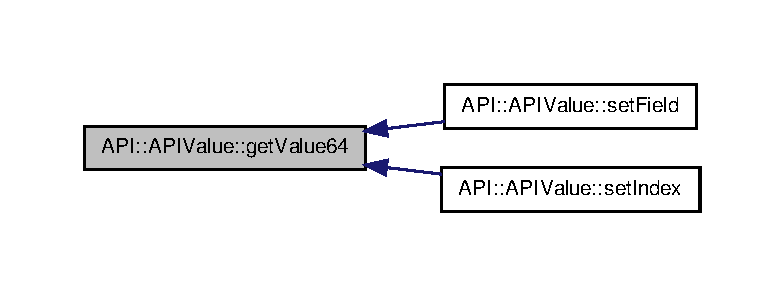
\includegraphics[width=350pt]{class_a_p_i_1_1_a_p_i_value_a26380a603f4fc9191608f047e6ea8250_icgraph}
\end{center}
\end{figure}


\hypertarget{class_a_p_i_1_1_a_p_i_value_a720e381988acbc87b34df8535d61e4d2}{\index{A\-P\-I\-::\-A\-P\-I\-Value@{A\-P\-I\-::\-A\-P\-I\-Value}!get\-Value\-Boolean@{get\-Value\-Boolean}}
\index{get\-Value\-Boolean@{get\-Value\-Boolean}!API::APIValue@{A\-P\-I\-::\-A\-P\-I\-Value}}
\subsubsection[{get\-Value\-Boolean}]{\setlength{\rightskip}{0pt plus 5cm}bool A\-P\-I\-::\-A\-P\-I\-Value\-::get\-Value\-Boolean (
\begin{DoxyParamCaption}
{}
\end{DoxyParamCaption}
)\hspace{0.3cm}{\ttfamily [inline]}}}\label{class_a_p_i_1_1_a_p_i_value_a720e381988acbc87b34df8535d61e4d2}
Returns true if the value is equal to V\-M\-::vm\-True ( The V\-Ms representation of a true boolean ) otherwise returns false. 

Definition at line 88 of file A\-P\-I\-Value.\-hpp.

\hypertarget{class_a_p_i_1_1_a_p_i_value_a2374ba437041f0c57514be649825312b}{\index{A\-P\-I\-::\-A\-P\-I\-Value@{A\-P\-I\-::\-A\-P\-I\-Value}!get\-Value\-Float32@{get\-Value\-Float32}}
\index{get\-Value\-Float32@{get\-Value\-Float32}!API::APIValue@{A\-P\-I\-::\-A\-P\-I\-Value}}
\subsubsection[{get\-Value\-Float32}]{\setlength{\rightskip}{0pt plus 5cm}{\bf float32\-\_\-t} A\-P\-I\-::\-A\-P\-I\-Value\-::get\-Value\-Float32 (
\begin{DoxyParamCaption}
{}
\end{DoxyParamCaption}
)\hspace{0.3cm}{\ttfamily [inline]}}}\label{class_a_p_i_1_1_a_p_i_value_a2374ba437041f0c57514be649825312b}
This returns the value as a 32 bit floating point number. 

Definition at line 72 of file A\-P\-I\-Value.\-hpp.



Here is the caller graph for this function\-:
\nopagebreak
\begin{figure}[H]
\begin{center}
\leavevmode
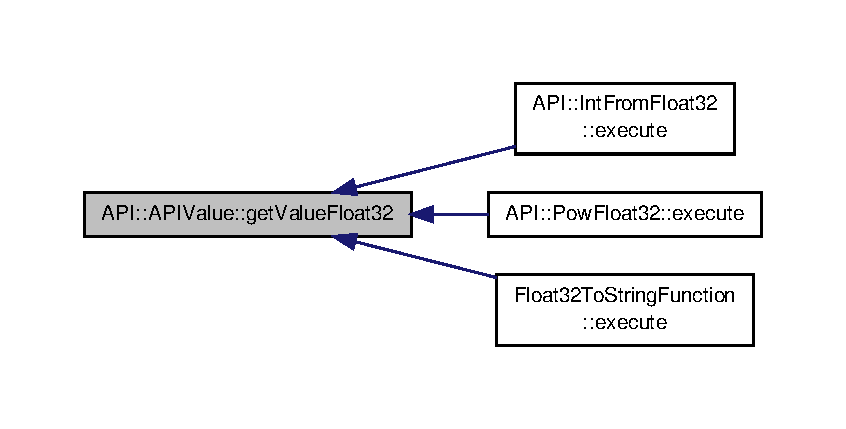
\includegraphics[width=350pt]{class_a_p_i_1_1_a_p_i_value_a2374ba437041f0c57514be649825312b_icgraph}
\end{center}
\end{figure}


\hypertarget{class_a_p_i_1_1_a_p_i_value_a94eb3d9f4b1c0dfd397f6813fd8c8a94}{\index{A\-P\-I\-::\-A\-P\-I\-Value@{A\-P\-I\-::\-A\-P\-I\-Value}!get\-Value\-String@{get\-Value\-String}}
\index{get\-Value\-String@{get\-Value\-String}!API::APIValue@{A\-P\-I\-::\-A\-P\-I\-Value}}
\subsubsection[{get\-Value\-String}]{\setlength{\rightskip}{0pt plus 5cm}char$\ast$ A\-P\-I\-::\-A\-P\-I\-Value\-::get\-Value\-String (
\begin{DoxyParamCaption}
{}
\end{DoxyParamCaption}
)\hspace{0.3cm}{\ttfamily [inline]}}}\label{class_a_p_i_1_1_a_p_i_value_a94eb3d9f4b1c0dfd397f6813fd8c8a94}
If the value is a string, return a pointer to the string. 

Definition at line 80 of file A\-P\-I\-Value.\-hpp.



Here is the call graph for this function\-:
\nopagebreak
\begin{figure}[H]
\begin{center}
\leavevmode
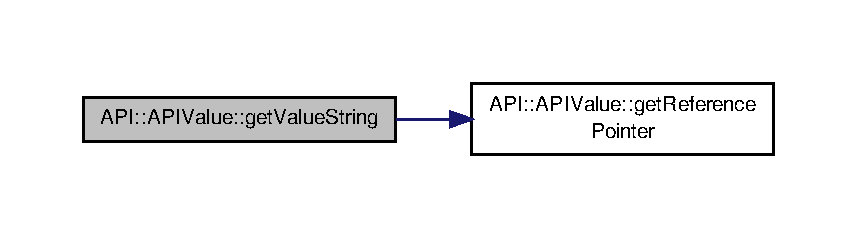
\includegraphics[width=350pt]{class_a_p_i_1_1_a_p_i_value_a94eb3d9f4b1c0dfd397f6813fd8c8a94_cgraph}
\end{center}
\end{figure}




Here is the caller graph for this function\-:
\nopagebreak
\begin{figure}[H]
\begin{center}
\leavevmode
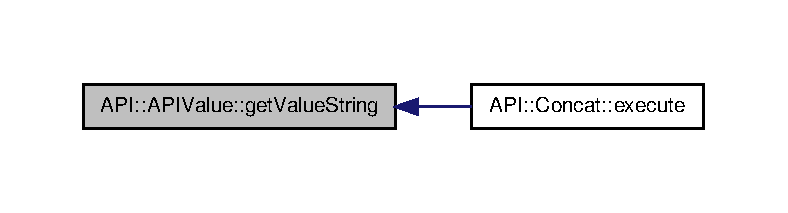
\includegraphics[width=350pt]{class_a_p_i_1_1_a_p_i_value_a94eb3d9f4b1c0dfd397f6813fd8c8a94_icgraph}
\end{center}
\end{figure}


\hypertarget{class_a_p_i_1_1_a_p_i_value_a8a97634f469ced8407f4ca6cdd0f9898}{\index{A\-P\-I\-::\-A\-P\-I\-Value@{A\-P\-I\-::\-A\-P\-I\-Value}!is\-Null@{is\-Null}}
\index{is\-Null@{is\-Null}!API::APIValue@{A\-P\-I\-::\-A\-P\-I\-Value}}
\subsubsection[{is\-Null}]{\setlength{\rightskip}{0pt plus 5cm}bool A\-P\-I\-::\-A\-P\-I\-Value\-::is\-Null (
\begin{DoxyParamCaption}
{}
\end{DoxyParamCaption}
)\hspace{0.3cm}{\ttfamily [inline]}}}\label{class_a_p_i_1_1_a_p_i_value_a8a97634f469ced8407f4ca6cdd0f9898}
Returns true if the register value is set to zero. 

Definition at line 134 of file A\-P\-I\-Value.\-hpp.



Here is the caller graph for this function\-:
\nopagebreak
\begin{figure}[H]
\begin{center}
\leavevmode
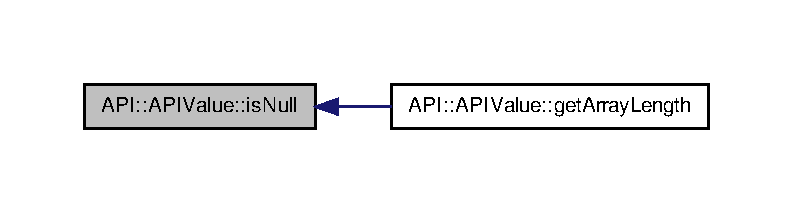
\includegraphics[width=350pt]{class_a_p_i_1_1_a_p_i_value_a8a97634f469ced8407f4ca6cdd0f9898_icgraph}
\end{center}
\end{figure}


\hypertarget{class_a_p_i_1_1_a_p_i_value_a9f5b34b9c70f6279dea8f556698ca1f6}{\index{A\-P\-I\-::\-A\-P\-I\-Value@{A\-P\-I\-::\-A\-P\-I\-Value}!is\-Reference@{is\-Reference}}
\index{is\-Reference@{is\-Reference}!API::APIValue@{A\-P\-I\-::\-A\-P\-I\-Value}}
\subsubsection[{is\-Reference}]{\setlength{\rightskip}{0pt plus 5cm}bool A\-P\-I\-::\-A\-P\-I\-Value\-::is\-Reference (
\begin{DoxyParamCaption}
{}
\end{DoxyParamCaption}
)\hspace{0.3cm}{\ttfamily [inline]}}}\label{class_a_p_i_1_1_a_p_i_value_a9f5b34b9c70f6279dea8f556698ca1f6}
Returns true if this \hyperlink{class_a_p_i_1_1_a_p_i_value}{A\-P\-I\-Value} is a reference to a piece of data on the heap. 

Definition at line 121 of file A\-P\-I\-Value.\-hpp.



Here is the caller graph for this function\-:
\nopagebreak
\begin{figure}[H]
\begin{center}
\leavevmode
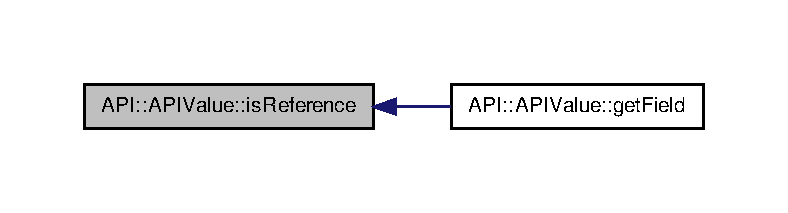
\includegraphics[width=350pt]{class_a_p_i_1_1_a_p_i_value_a9f5b34b9c70f6279dea8f556698ca1f6_icgraph}
\end{center}
\end{figure}


\hypertarget{class_a_p_i_1_1_a_p_i_value_ae4d8ca7c8a72f24e3b7419cc4fc2127c}{\index{A\-P\-I\-::\-A\-P\-I\-Value@{A\-P\-I\-::\-A\-P\-I\-Value}!make\-Float32@{make\-Float32}}
\index{make\-Float32@{make\-Float32}!API::APIValue@{A\-P\-I\-::\-A\-P\-I\-Value}}
\subsubsection[{make\-Float32}]{\setlength{\rightskip}{0pt plus 5cm}static {\bf A\-P\-I\-::\-A\-P\-I\-Value} A\-P\-I\-::\-A\-P\-I\-Value\-::make\-Float32 (
\begin{DoxyParamCaption}
\item[{{\bf float32\-\_\-t}}]{val}
\end{DoxyParamCaption}
)\hspace{0.3cm}{\ttfamily [inline]}, {\ttfamily [static]}}}\label{class_a_p_i_1_1_a_p_i_value_ae4d8ca7c8a72f24e3b7419cc4fc2127c}


Definition at line 352 of file A\-P\-I\-Value.\-hpp.



Here is the call graph for this function\-:
\nopagebreak
\begin{figure}[H]
\begin{center}
\leavevmode
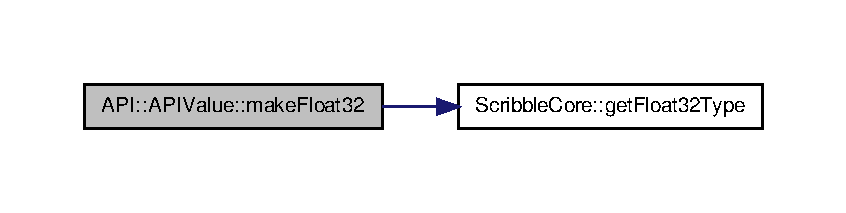
\includegraphics[width=350pt]{class_a_p_i_1_1_a_p_i_value_ae4d8ca7c8a72f24e3b7419cc4fc2127c_cgraph}
\end{center}
\end{figure}




Here is the caller graph for this function\-:
\nopagebreak
\begin{figure}[H]
\begin{center}
\leavevmode
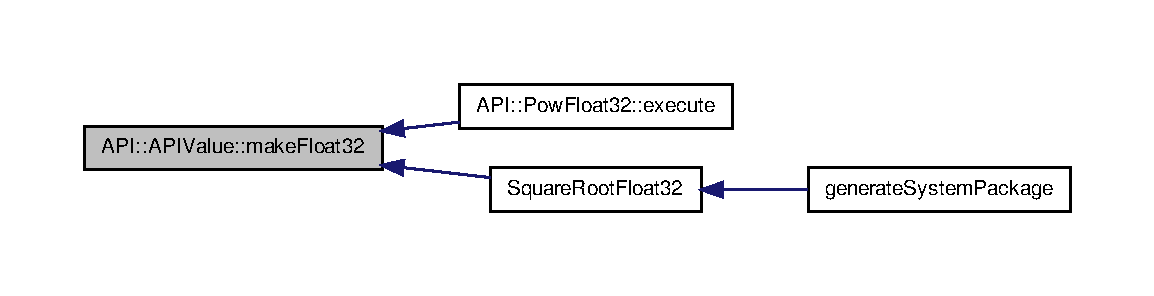
\includegraphics[width=350pt]{class_a_p_i_1_1_a_p_i_value_ae4d8ca7c8a72f24e3b7419cc4fc2127c_icgraph}
\end{center}
\end{figure}


\hypertarget{class_a_p_i_1_1_a_p_i_value_a5d2ee6a2550a35698b7f63678c64fc47}{\index{A\-P\-I\-::\-A\-P\-I\-Value@{A\-P\-I\-::\-A\-P\-I\-Value}!make\-Int32@{make\-Int32}}
\index{make\-Int32@{make\-Int32}!API::APIValue@{A\-P\-I\-::\-A\-P\-I\-Value}}
\subsubsection[{make\-Int32}]{\setlength{\rightskip}{0pt plus 5cm}static {\bf A\-P\-I\-::\-A\-P\-I\-Value} A\-P\-I\-::\-A\-P\-I\-Value\-::make\-Int32 (
\begin{DoxyParamCaption}
\item[{int}]{val}
\end{DoxyParamCaption}
)\hspace{0.3cm}{\ttfamily [inline]}, {\ttfamily [static]}}}\label{class_a_p_i_1_1_a_p_i_value_a5d2ee6a2550a35698b7f63678c64fc47}


Definition at line 348 of file A\-P\-I\-Value.\-hpp.



Here is the call graph for this function\-:
\nopagebreak
\begin{figure}[H]
\begin{center}
\leavevmode
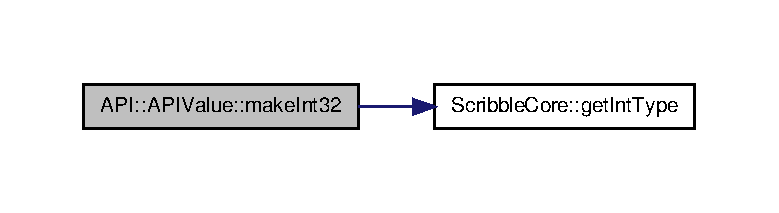
\includegraphics[width=350pt]{class_a_p_i_1_1_a_p_i_value_a5d2ee6a2550a35698b7f63678c64fc47_cgraph}
\end{center}
\end{figure}




Here is the caller graph for this function\-:
\nopagebreak
\begin{figure}[H]
\begin{center}
\leavevmode
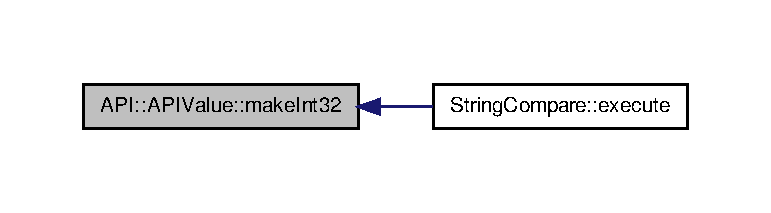
\includegraphics[width=350pt]{class_a_p_i_1_1_a_p_i_value_a5d2ee6a2550a35698b7f63678c64fc47_icgraph}
\end{center}
\end{figure}


\hypertarget{class_a_p_i_1_1_a_p_i_value_abc6491d068cfc443ef5cbbc83156e46e}{\index{A\-P\-I\-::\-A\-P\-I\-Value@{A\-P\-I\-::\-A\-P\-I\-Value}!make\-String@{make\-String}}
\index{make\-String@{make\-String}!API::APIValue@{A\-P\-I\-::\-A\-P\-I\-Value}}
\subsubsection[{make\-String}]{\setlength{\rightskip}{0pt plus 5cm}static {\bf A\-P\-I\-::\-A\-P\-I\-Value} A\-P\-I\-::\-A\-P\-I\-Value\-::make\-String (
\begin{DoxyParamCaption}
\item[{std\-::string const \&}]{text, }
\item[{{\bf V\-M\-::\-Virtual\-Machine} $\ast$}]{vm}
\end{DoxyParamCaption}
)\hspace{0.3cm}{\ttfamily [inline]}, {\ttfamily [static]}}}\label{class_a_p_i_1_1_a_p_i_value_abc6491d068cfc443ef5cbbc83156e46e}


Definition at line 356 of file A\-P\-I\-Value.\-hpp.



Here is the call graph for this function\-:
\nopagebreak
\begin{figure}[H]
\begin{center}
\leavevmode
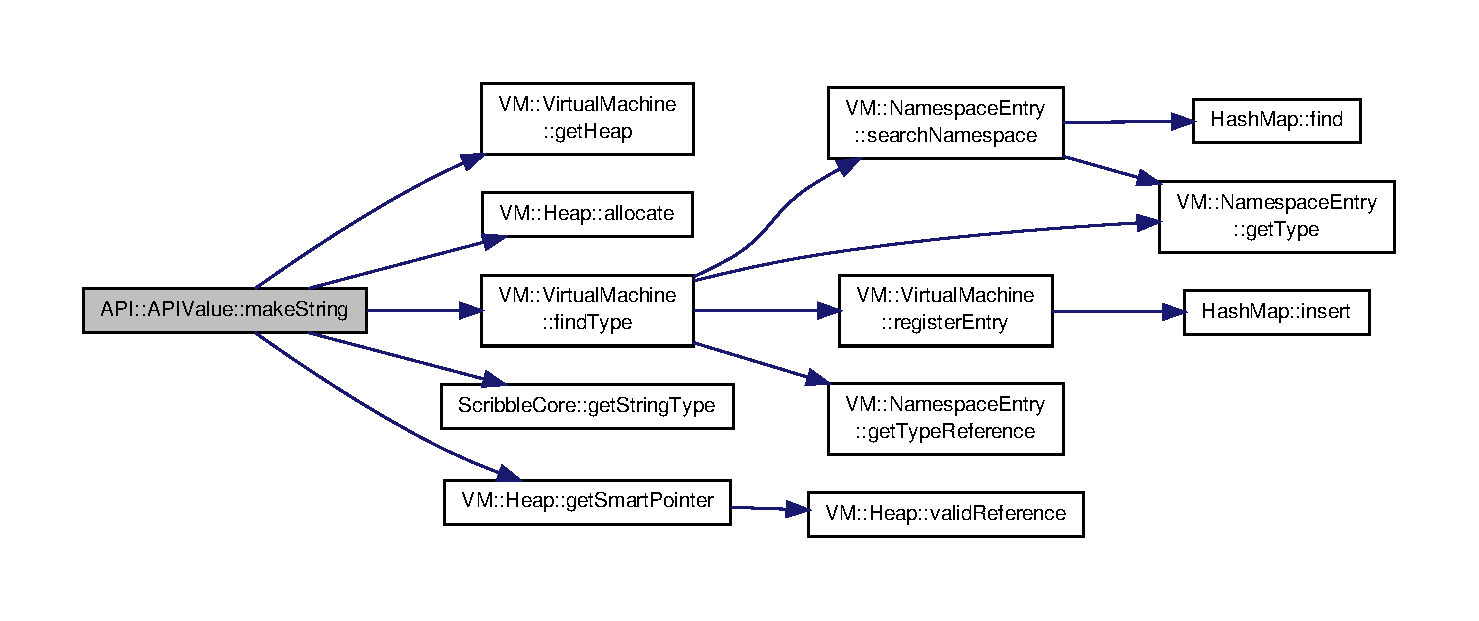
\includegraphics[width=350pt]{class_a_p_i_1_1_a_p_i_value_abc6491d068cfc443ef5cbbc83156e46e_cgraph}
\end{center}
\end{figure}




Here is the caller graph for this function\-:
\nopagebreak
\begin{figure}[H]
\begin{center}
\leavevmode
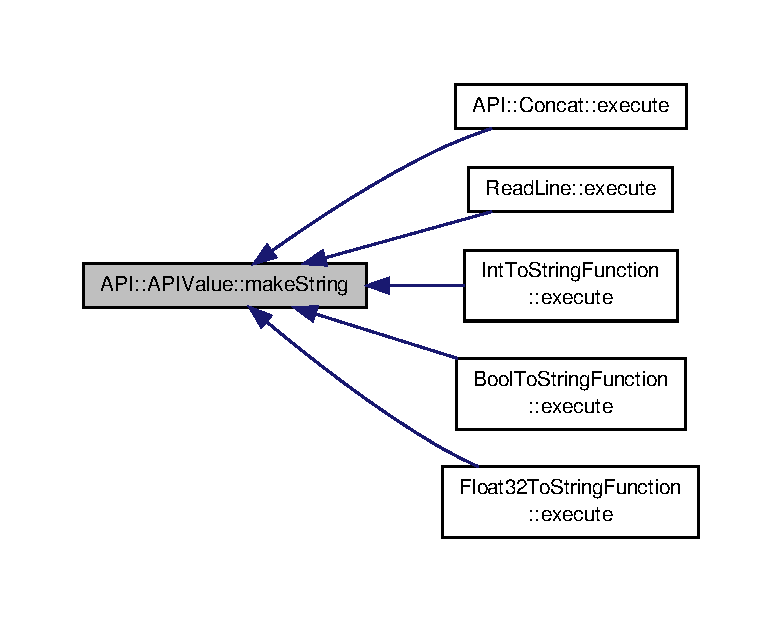
\includegraphics[width=350pt]{class_a_p_i_1_1_a_p_i_value_abc6491d068cfc443ef5cbbc83156e46e_icgraph}
\end{center}
\end{figure}


\hypertarget{class_a_p_i_1_1_a_p_i_value_a54a170b1214ed9daf309c889b7daf77e}{\index{A\-P\-I\-::\-A\-P\-I\-Value@{A\-P\-I\-::\-A\-P\-I\-Value}!push\-To\-V\-M@{push\-To\-V\-M}}
\index{push\-To\-V\-M@{push\-To\-V\-M}!API::APIValue@{A\-P\-I\-::\-A\-P\-I\-Value}}
\subsubsection[{push\-To\-V\-M}]{\setlength{\rightskip}{0pt plus 5cm}void A\-P\-I\-::\-A\-P\-I\-Value\-::push\-To\-V\-M (
\begin{DoxyParamCaption}
\item[{{\bf V\-M\-::\-Virtual\-Machine} $\ast$}]{virt}
\end{DoxyParamCaption}
)\hspace{0.3cm}{\ttfamily [inline]}}}\label{class_a_p_i_1_1_a_p_i_value_a54a170b1214ed9daf309c889b7daf77e}


Definition at line 339 of file A\-P\-I\-Value.\-hpp.



Here is the call graph for this function\-:
\nopagebreak
\begin{figure}[H]
\begin{center}
\leavevmode
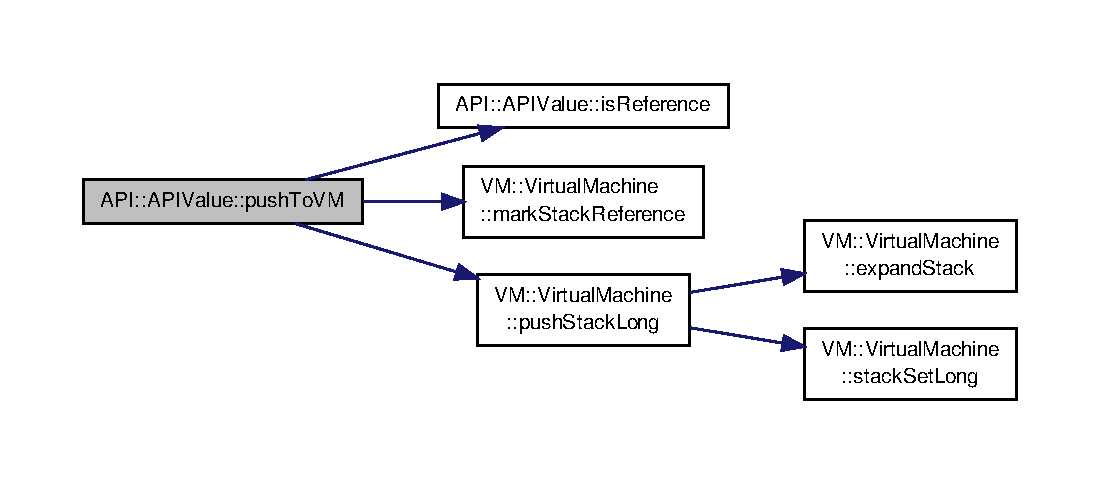
\includegraphics[width=350pt]{class_a_p_i_1_1_a_p_i_value_a54a170b1214ed9daf309c889b7daf77e_cgraph}
\end{center}
\end{figure}


\hypertarget{class_a_p_i_1_1_a_p_i_value_aa516e6d20f842e2dfd60c1c59a697312}{\index{A\-P\-I\-::\-A\-P\-I\-Value@{A\-P\-I\-::\-A\-P\-I\-Value}!set\-Field@{set\-Field}}
\index{set\-Field@{set\-Field}!API::APIValue@{A\-P\-I\-::\-A\-P\-I\-Value}}
\subsubsection[{set\-Field}]{\setlength{\rightskip}{0pt plus 5cm}void A\-P\-I\-::\-A\-P\-I\-Value\-::set\-Field (
\begin{DoxyParamCaption}
\item[{std\-::string const \&}]{name, }
\item[{{\bf A\-P\-I\-::\-A\-P\-I\-Value}}]{val, }
\item[{{\bf V\-M\-::\-Virtual\-Machine} $\ast$}]{vm}
\end{DoxyParamCaption}
)\hspace{0.3cm}{\ttfamily [inline]}}}\label{class_a_p_i_1_1_a_p_i_value_aa516e6d20f842e2dfd60c1c59a697312}


Definition at line 261 of file A\-P\-I\-Value.\-hpp.



Here is the call graph for this function\-:
\nopagebreak
\begin{figure}[H]
\begin{center}
\leavevmode
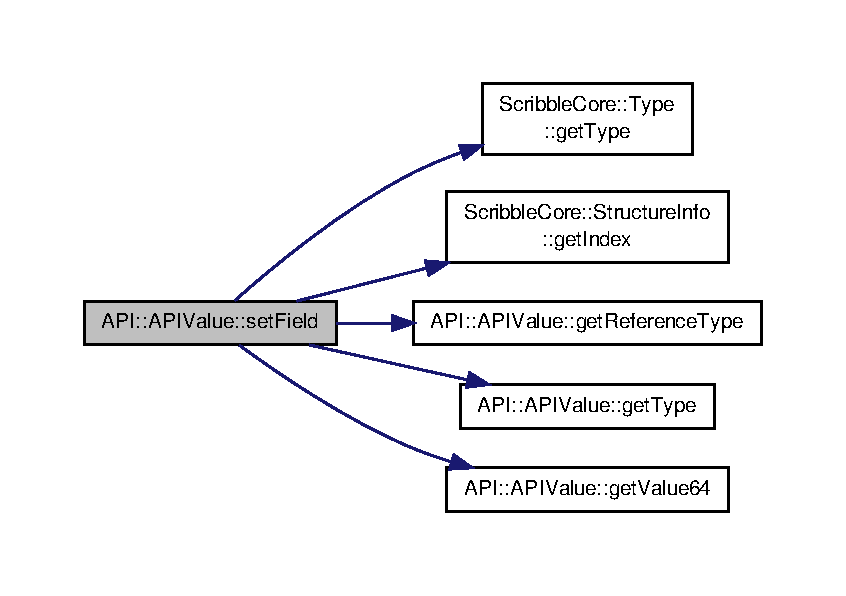
\includegraphics[width=350pt]{class_a_p_i_1_1_a_p_i_value_aa516e6d20f842e2dfd60c1c59a697312_cgraph}
\end{center}
\end{figure}


\hypertarget{class_a_p_i_1_1_a_p_i_value_aa8a379bf602fc10523bfc4a4867dbc55}{\index{A\-P\-I\-::\-A\-P\-I\-Value@{A\-P\-I\-::\-A\-P\-I\-Value}!set\-Index@{set\-Index}}
\index{set\-Index@{set\-Index}!API::APIValue@{A\-P\-I\-::\-A\-P\-I\-Value}}
\subsubsection[{set\-Index}]{\setlength{\rightskip}{0pt plus 5cm}void A\-P\-I\-::\-A\-P\-I\-Value\-::set\-Index (
\begin{DoxyParamCaption}
\item[{unsigned int}]{index, }
\item[{{\bf A\-P\-I\-::\-A\-P\-I\-Value}}]{val, }
\item[{{\bf V\-M\-::\-Virtual\-Machine} $\ast$}]{vm}
\end{DoxyParamCaption}
)\hspace{0.3cm}{\ttfamily [inline]}}}\label{class_a_p_i_1_1_a_p_i_value_aa8a379bf602fc10523bfc4a4867dbc55}


Definition at line 301 of file A\-P\-I\-Value.\-hpp.



Here is the call graph for this function\-:
\nopagebreak
\begin{figure}[H]
\begin{center}
\leavevmode
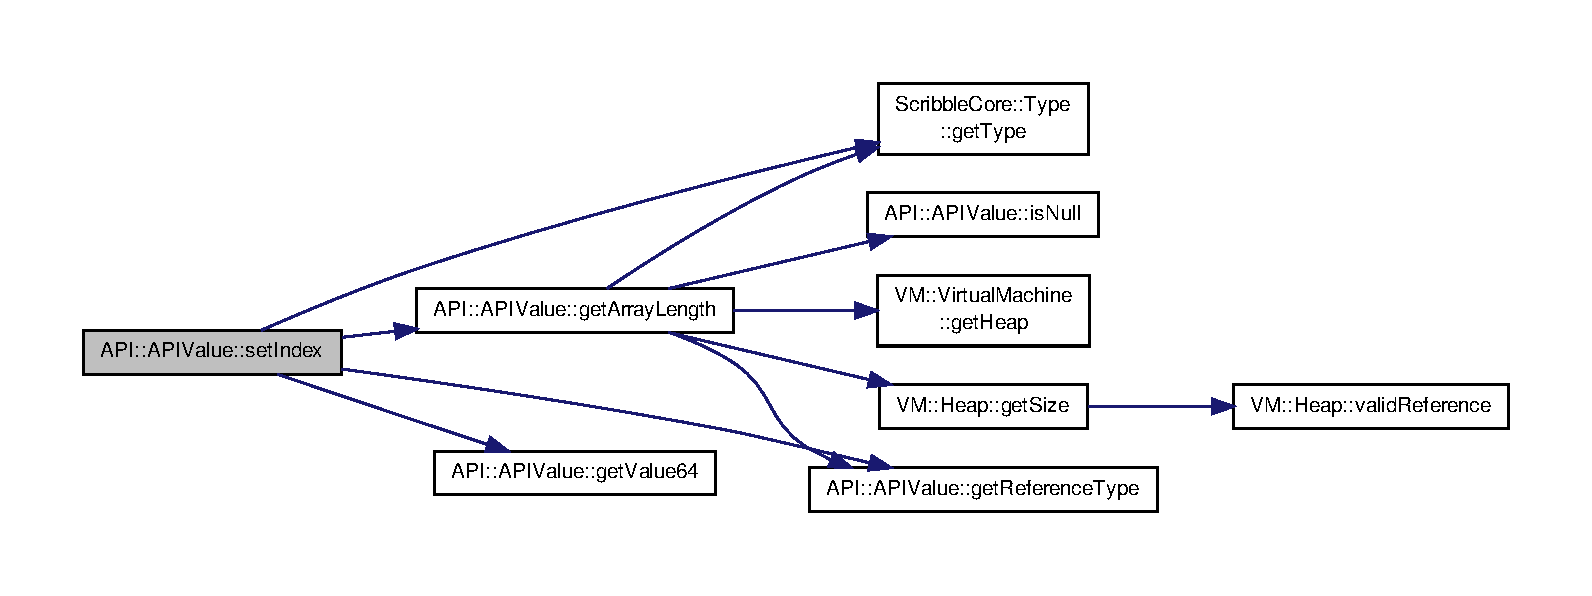
\includegraphics[width=350pt]{class_a_p_i_1_1_a_p_i_value_aa8a379bf602fc10523bfc4a4867dbc55_cgraph}
\end{center}
\end{figure}




The documentation for this class was generated from the following files\-:\begin{DoxyCompactItemize}
\item 
/home/blake/\-Dropbox/\-Current/\-Scribble/src/\-A\-P\-I/\-Value/\hyperlink{_a_p_i_value_8hpp}{A\-P\-I\-Value.\-hpp}\item 
/home/blake/\-Dropbox/\-Current/\-Scribble/src/\-A\-P\-I/\-Value/\hyperlink{_a_p_i_value_8cpp}{A\-P\-I\-Value.\-cpp}\end{DoxyCompactItemize}

\hypertarget{class_scribble_core_1_1_array_length_statement}{\section{Scribble\-Core\-:\-:Array\-Length\-Statement Class Reference}
\label{class_scribble_core_1_1_array_length_statement}\index{Scribble\-Core\-::\-Array\-Length\-Statement@{Scribble\-Core\-::\-Array\-Length\-Statement}}
}


{\ttfamily \#include $<$Array\-Length\-Statement.\-hpp$>$}



Inheritance diagram for Scribble\-Core\-:\-:Array\-Length\-Statement\-:\nopagebreak
\begin{figure}[H]
\begin{center}
\leavevmode
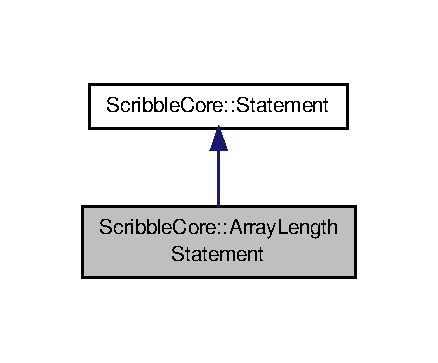
\includegraphics[width=210pt]{class_scribble_core_1_1_array_length_statement__inherit__graph}
\end{center}
\end{figure}


Collaboration diagram for Scribble\-Core\-:\-:Array\-Length\-Statement\-:\nopagebreak
\begin{figure}[H]
\begin{center}
\leavevmode
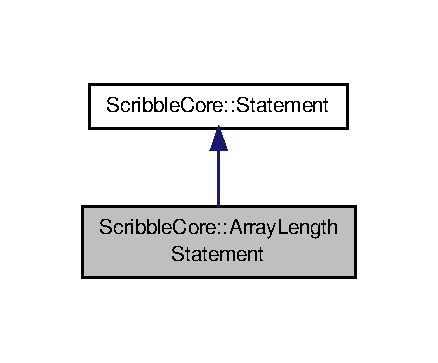
\includegraphics[width=210pt]{class_scribble_core_1_1_array_length_statement__coll__graph}
\end{center}
\end{figure}
\subsection*{Public Member Functions}
\begin{DoxyCompactItemize}
\item 
\hyperlink{class_scribble_core_1_1_array_length_statement_a0f373eaf826db2565073f5da6b7d3de7}{Array\-Length\-Statement} (int line, std\-::string text, Safe\-Statement exp)
\item 
\hypertarget{class_scribble_core_1_1_array_length_statement_a7861cbb5791ce1d651dad677f000e757}{virtual void {\bfseries check\-Tree} (\hyperlink{class_scribble_core_1_1_type}{Type} $\ast$function\-Type)}\label{class_scribble_core_1_1_array_length_statement_a7861cbb5791ce1d651dad677f000e757}

\item 
\hypertarget{class_scribble_core_1_1_array_length_statement_ae47bb975e562d05b1c3da60b3f7e40aa}{virtual int {\bfseries generate\-Code} (int result\-Register, std\-::stringstream \&generated)}\label{class_scribble_core_1_1_array_length_statement_ae47bb975e562d05b1c3da60b3f7e40aa}

\item 
virtual \hyperlink{class_scribble_core_1_1_type}{Type} $\ast$ \hyperlink{class_scribble_core_1_1_array_length_statement_ac7c1deececdad51dc373ce4942f99ddc}{type} ()
\end{DoxyCompactItemize}


\subsection{Detailed Description}
This statement takes a statement which returns an array and returns the length of that array. 

\subsection{Constructor \& Destructor Documentation}
\hypertarget{class_scribble_core_1_1_array_length_statement_a0f373eaf826db2565073f5da6b7d3de7}{\index{Scribble\-Core\-::\-Array\-Length\-Statement@{Scribble\-Core\-::\-Array\-Length\-Statement}!Array\-Length\-Statement@{Array\-Length\-Statement}}
\index{Array\-Length\-Statement@{Array\-Length\-Statement}!ScribbleCore::ArrayLengthStatement@{Scribble\-Core\-::\-Array\-Length\-Statement}}
\subsubsection[{Array\-Length\-Statement}]{\setlength{\rightskip}{0pt plus 5cm}Scribble\-Core\-::\-Array\-Length\-Statement\-::\-Array\-Length\-Statement (
\begin{DoxyParamCaption}
\item[{int}]{line, }
\item[{std\-::string}]{text, }
\item[{Safe\-Statement}]{exp}
\end{DoxyParamCaption}
)}}\label{class_scribble_core_1_1_array_length_statement_a0f373eaf826db2565073f5da6b7d3de7}
Construct an array length statement. 
\begin{DoxyParams}{Parameters}
{\em line} & The line number on which the line occurs. \\
\hline
{\em text} & The The symbol in which this statement occurs. \\
\hline
{\em exp} & The array expression. \\
\hline
\end{DoxyParams}


\subsection{Member Function Documentation}
\hypertarget{class_scribble_core_1_1_array_length_statement_ac7c1deececdad51dc373ce4942f99ddc}{\index{Scribble\-Core\-::\-Array\-Length\-Statement@{Scribble\-Core\-::\-Array\-Length\-Statement}!type@{type}}
\index{type@{type}!ScribbleCore::ArrayLengthStatement@{Scribble\-Core\-::\-Array\-Length\-Statement}}
\subsubsection[{type}]{\setlength{\rightskip}{0pt plus 5cm}{\bf Type} $\ast$ Scribble\-Core\-::\-Array\-Length\-Statement\-::type (
\begin{DoxyParamCaption}
{}
\end{DoxyParamCaption}
)\hspace{0.3cm}{\ttfamily [virtual]}}}\label{class_scribble_core_1_1_array_length_statement_ac7c1deececdad51dc373ce4942f99ddc}
The type will be an integer. \begin{DoxyReturn}{Returns}
The int type. 
\end{DoxyReturn}


Implements \hyperlink{class_scribble_core_1_1_statement}{Scribble\-Core\-::\-Statement}.



The documentation for this class was generated from the following files\-:\begin{DoxyCompactItemize}
\item 
/home/blake/\-Dropbox/\-Current/\-Scribble/src/\-Scribble/\-Statement/Array\-Length\-Statement.\-hpp\item 
/home/blake/\-Dropbox/\-Current/\-Scribble/src/\-Scribble/\-Statement/Array\-Length\-Statement.\-cpp\end{DoxyCompactItemize}

\hypertarget{class_scribble_core_1_1_array_statement}{\section{Scribble\-Core\-:\-:Array\-Statement Class Reference}
\label{class_scribble_core_1_1_array_statement}\index{Scribble\-Core\-::\-Array\-Statement@{Scribble\-Core\-::\-Array\-Statement}}
}


{\ttfamily \#include $<$Array\-Statement.\-hpp$>$}



Inheritance diagram for Scribble\-Core\-:\-:Array\-Statement\-:
\nopagebreak
\begin{figure}[H]
\begin{center}
\leavevmode
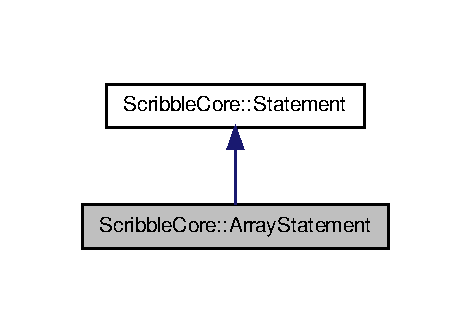
\includegraphics[width=226pt]{class_scribble_core_1_1_array_statement__inherit__graph}
\end{center}
\end{figure}


Collaboration diagram for Scribble\-Core\-:\-:Array\-Statement\-:
\nopagebreak
\begin{figure}[H]
\begin{center}
\leavevmode
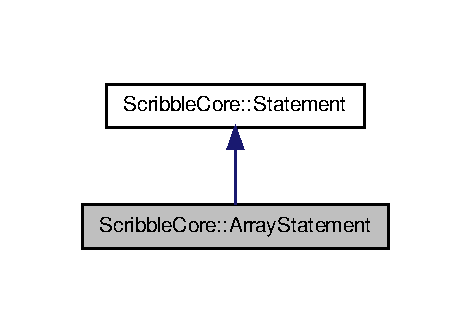
\includegraphics[width=226pt]{class_scribble_core_1_1_array_statement__coll__graph}
\end{center}
\end{figure}
\subsection*{Public Member Functions}
\begin{DoxyCompactItemize}
\item 
\hyperlink{class_scribble_core_1_1_array_statement_a0decfb9a7c6f44fd2715180caed7565c}{Array\-Statement} (int line, std\-::string text, \hyperlink{class_scribble_core_1_1_type}{Type} $\ast$\hyperlink{class_scribble_core_1_1_array_statement_a5b54b69993960b2dbaac9c49a25e6617}{type}, \hyperlink{namespace_scribble_core_a2ad5bf236bc9164cb56f564685f15a11}{Safe\-Statement} length)
\item 
virtual \hyperlink{class_scribble_core_1_1_array_statement_a737a24ca0c8806612e94ac037314eb5c}{$\sim$\-Array\-Statement} ()
\item 
\hyperlink{class_scribble_core_1_1_type}{Type} $\ast$ \hyperlink{class_scribble_core_1_1_array_statement_a5b54b69993960b2dbaac9c49a25e6617}{type} ()
\item 
void \hyperlink{class_scribble_core_1_1_array_statement_a4e4ea1be352a79a9749b057e67921c52}{check\-Tree} (\hyperlink{class_scribble_core_1_1_type}{Type} $\ast$function\-Type)
\item 
int \hyperlink{class_scribble_core_1_1_array_statement_aa5ac3da5af213e1c34092ab4a091a83e}{generate\-Code} (int result\-Register, std\-::stringstream \&generated)
\end{DoxyCompactItemize}


\subsection{Detailed Description}
\hyperlink{class_scribble_core_1_1_array_statement}{Array\-Statement} which returns a new Array of length returned by the supplied statement. 

Definition at line 18 of file Array\-Statement.\-hpp.



\subsection{Constructor \& Destructor Documentation}
\hypertarget{class_scribble_core_1_1_array_statement_a0decfb9a7c6f44fd2715180caed7565c}{\index{Scribble\-Core\-::\-Array\-Statement@{Scribble\-Core\-::\-Array\-Statement}!Array\-Statement@{Array\-Statement}}
\index{Array\-Statement@{Array\-Statement}!ScribbleCore::ArrayStatement@{Scribble\-Core\-::\-Array\-Statement}}
\subsubsection[{Array\-Statement}]{\setlength{\rightskip}{0pt plus 5cm}Scribble\-Core\-::\-Array\-Statement\-::\-Array\-Statement (
\begin{DoxyParamCaption}
\item[{int}]{line, }
\item[{std\-::string}]{text, }
\item[{{\bf Type} $\ast$}]{type, }
\item[{{\bf Safe\-Statement}}]{length}
\end{DoxyParamCaption}
)}}\label{class_scribble_core_1_1_array_statement_a0decfb9a7c6f44fd2715180caed7565c}
Construct array statement. 
\begin{DoxyParams}{Parameters}
{\em line} & The line number. \\
\hline
{\em text} & The symbol it occurs at. \\
\hline
{\em type} & The type of array to be generated. \\
\hline
{\em length} & The statement which returns the length. \\
\hline
\end{DoxyParams}


Definition at line 15 of file Array\-Statement.\-cpp.

\hypertarget{class_scribble_core_1_1_array_statement_a737a24ca0c8806612e94ac037314eb5c}{\index{Scribble\-Core\-::\-Array\-Statement@{Scribble\-Core\-::\-Array\-Statement}!$\sim$\-Array\-Statement@{$\sim$\-Array\-Statement}}
\index{$\sim$\-Array\-Statement@{$\sim$\-Array\-Statement}!ScribbleCore::ArrayStatement@{Scribble\-Core\-::\-Array\-Statement}}
\subsubsection[{$\sim$\-Array\-Statement}]{\setlength{\rightskip}{0pt plus 5cm}Scribble\-Core\-::\-Array\-Statement\-::$\sim$\-Array\-Statement (
\begin{DoxyParamCaption}
{}
\end{DoxyParamCaption}
)\hspace{0.3cm}{\ttfamily [virtual]}}}\label{class_scribble_core_1_1_array_statement_a737a24ca0c8806612e94ac037314eb5c}


Definition at line 20 of file Array\-Statement.\-cpp.



\subsection{Member Function Documentation}
\hypertarget{class_scribble_core_1_1_array_statement_a4e4ea1be352a79a9749b057e67921c52}{\index{Scribble\-Core\-::\-Array\-Statement@{Scribble\-Core\-::\-Array\-Statement}!check\-Tree@{check\-Tree}}
\index{check\-Tree@{check\-Tree}!ScribbleCore::ArrayStatement@{Scribble\-Core\-::\-Array\-Statement}}
\subsubsection[{check\-Tree}]{\setlength{\rightskip}{0pt plus 5cm}void Scribble\-Core\-::\-Array\-Statement\-::check\-Tree (
\begin{DoxyParamCaption}
\item[{{\bf Type} $\ast$}]{function\-Type}
\end{DoxyParamCaption}
)\hspace{0.3cm}{\ttfamily [virtual]}}}\label{class_scribble_core_1_1_array_statement_a4e4ea1be352a79a9749b057e67921c52}


Implements \hyperlink{class_scribble_core_1_1_statement_a894e4f8d8b35279bb9ea87f20afdb978}{Scribble\-Core\-::\-Statement}.



Definition at line 28 of file Array\-Statement.\-cpp.

\hypertarget{class_scribble_core_1_1_array_statement_aa5ac3da5af213e1c34092ab4a091a83e}{\index{Scribble\-Core\-::\-Array\-Statement@{Scribble\-Core\-::\-Array\-Statement}!generate\-Code@{generate\-Code}}
\index{generate\-Code@{generate\-Code}!ScribbleCore::ArrayStatement@{Scribble\-Core\-::\-Array\-Statement}}
\subsubsection[{generate\-Code}]{\setlength{\rightskip}{0pt plus 5cm}int Scribble\-Core\-::\-Array\-Statement\-::generate\-Code (
\begin{DoxyParamCaption}
\item[{int}]{result\-Register, }
\item[{std\-::stringstream \&}]{generated}
\end{DoxyParamCaption}
)\hspace{0.3cm}{\ttfamily [virtual]}}}\label{class_scribble_core_1_1_array_statement_aa5ac3da5af213e1c34092ab4a091a83e}


Reimplemented from \hyperlink{class_scribble_core_1_1_statement_aa3951ffef06ca195054a0bdfc8a4c8de}{Scribble\-Core\-::\-Statement}.



Definition at line 38 of file Array\-Statement.\-cpp.



Here is the call graph for this function\-:
\nopagebreak
\begin{figure}[H]
\begin{center}
\leavevmode
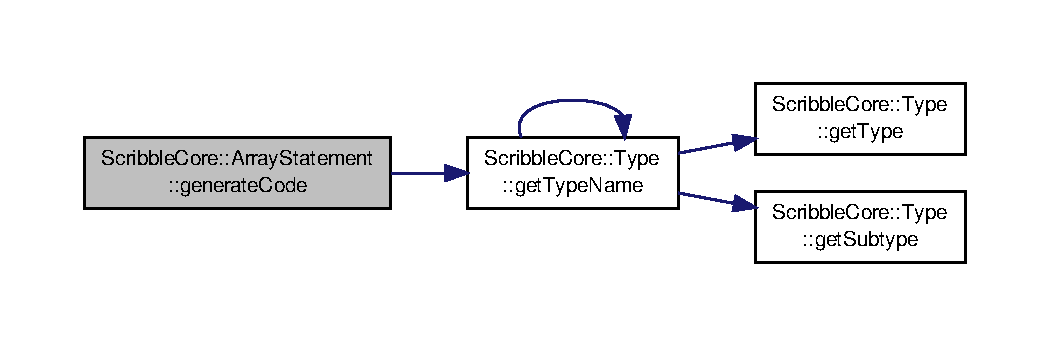
\includegraphics[width=350pt]{class_scribble_core_1_1_array_statement_aa5ac3da5af213e1c34092ab4a091a83e_cgraph}
\end{center}
\end{figure}


\hypertarget{class_scribble_core_1_1_array_statement_a5b54b69993960b2dbaac9c49a25e6617}{\index{Scribble\-Core\-::\-Array\-Statement@{Scribble\-Core\-::\-Array\-Statement}!type@{type}}
\index{type@{type}!ScribbleCore::ArrayStatement@{Scribble\-Core\-::\-Array\-Statement}}
\subsubsection[{type}]{\setlength{\rightskip}{0pt plus 5cm}{\bf Type} $\ast$ Scribble\-Core\-::\-Array\-Statement\-::type (
\begin{DoxyParamCaption}
{}
\end{DoxyParamCaption}
)\hspace{0.3cm}{\ttfamily [virtual]}}}\label{class_scribble_core_1_1_array_statement_a5b54b69993960b2dbaac9c49a25e6617}
Returns Array type. \begin{DoxyReturn}{Returns}
Array. 
\end{DoxyReturn}


Implements \hyperlink{class_scribble_core_1_1_statement_a532ed5a44ec49873dc191dae7ddc8b00}{Scribble\-Core\-::\-Statement}.



Definition at line 24 of file Array\-Statement.\-cpp.



The documentation for this class was generated from the following files\-:\begin{DoxyCompactItemize}
\item 
/home/blake/\-Dropbox/\-Current/\-Scribble/src/\-Scribble/\-Statement/\hyperlink{_array_statement_8hpp}{Array\-Statement.\-hpp}\item 
/home/blake/\-Dropbox/\-Current/\-Scribble/src/\-Scribble/\-Statement/\hyperlink{_array_statement_8cpp}{Array\-Statement.\-cpp}\end{DoxyCompactItemize}

\hypertarget{class_scribble_core_1_1_assign_array_statement}{\section{Scribble\-Core\-:\-:Assign\-Array\-Statement Class Reference}
\label{class_scribble_core_1_1_assign_array_statement}\index{Scribble\-Core\-::\-Assign\-Array\-Statement@{Scribble\-Core\-::\-Assign\-Array\-Statement}}
}


{\ttfamily \#include $<$Assign\-Array\-Statement.\-hpp$>$}



Inheritance diagram for Scribble\-Core\-:\-:Assign\-Array\-Statement\-:\nopagebreak
\begin{figure}[H]
\begin{center}
\leavevmode
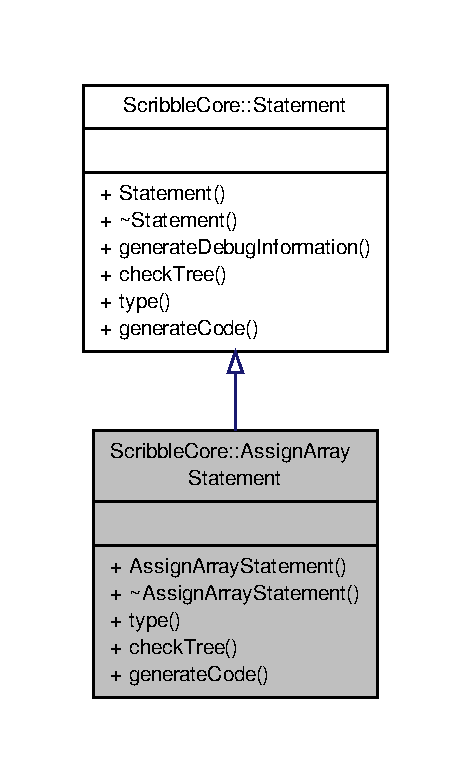
\includegraphics[width=212pt]{class_scribble_core_1_1_assign_array_statement__inherit__graph}
\end{center}
\end{figure}


Collaboration diagram for Scribble\-Core\-:\-:Assign\-Array\-Statement\-:\nopagebreak
\begin{figure}[H]
\begin{center}
\leavevmode
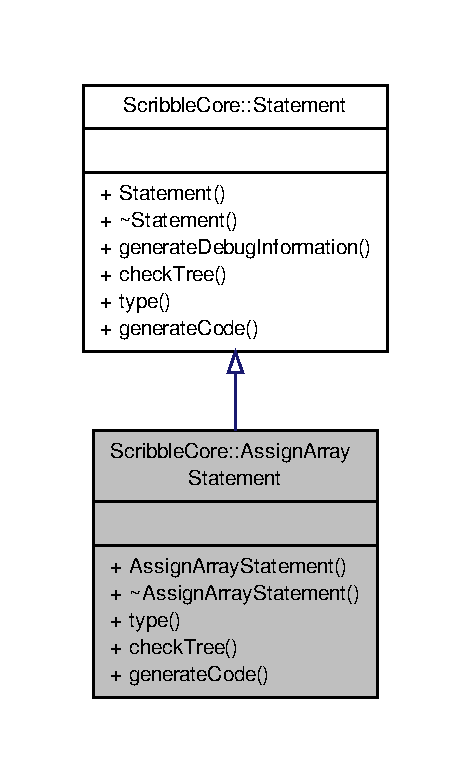
\includegraphics[width=212pt]{class_scribble_core_1_1_assign_array_statement__coll__graph}
\end{center}
\end{figure}
\subsection*{Public Member Functions}
\begin{DoxyCompactItemize}
\item 
\hyperlink{class_scribble_core_1_1_assign_array_statement_a1ee1ce9e49bb0c1c03f80cfb8e5d115d}{Assign\-Array\-Statement} (int lineno, std\-::string text, Safe\-Statement array, Safe\-Statement assign, Safe\-Statement position)
\item 
\hyperlink{class_scribble_core_1_1_type}{Type} $\ast$ \hyperlink{class_scribble_core_1_1_assign_array_statement_ac178b7f29bff1248d3a88023ae47eb96}{type} ()
\item 
\hypertarget{class_scribble_core_1_1_assign_array_statement_a5346d4acadb05916f47da731f23f70ef}{void {\bfseries check\-Tree} (\hyperlink{class_scribble_core_1_1_type}{Type} $\ast$function\-Type)}\label{class_scribble_core_1_1_assign_array_statement_a5346d4acadb05916f47da731f23f70ef}

\item 
\hypertarget{class_scribble_core_1_1_assign_array_statement_a53d2ef3cb8185606f678d7d60a8da426}{int {\bfseries generate\-Code} (int result\-Register, std\-::stringstream \&generated)}\label{class_scribble_core_1_1_assign_array_statement_a53d2ef3cb8185606f678d7d60a8da426}

\end{DoxyCompactItemize}


\subsection{Detailed Description}
Assigns element assign at the specified position in the given array. 

\subsection{Constructor \& Destructor Documentation}
\hypertarget{class_scribble_core_1_1_assign_array_statement_a1ee1ce9e49bb0c1c03f80cfb8e5d115d}{\index{Scribble\-Core\-::\-Assign\-Array\-Statement@{Scribble\-Core\-::\-Assign\-Array\-Statement}!Assign\-Array\-Statement@{Assign\-Array\-Statement}}
\index{Assign\-Array\-Statement@{Assign\-Array\-Statement}!ScribbleCore::AssignArrayStatement@{Scribble\-Core\-::\-Assign\-Array\-Statement}}
\subsubsection[{Assign\-Array\-Statement}]{\setlength{\rightskip}{0pt plus 5cm}Scribble\-Core\-::\-Assign\-Array\-Statement\-::\-Assign\-Array\-Statement (
\begin{DoxyParamCaption}
\item[{int}]{lineno, }
\item[{std\-::string}]{text, }
\item[{Safe\-Statement}]{array, }
\item[{Safe\-Statement}]{assign, }
\item[{Safe\-Statement}]{position}
\end{DoxyParamCaption}
)}}\label{class_scribble_core_1_1_assign_array_statement_a1ee1ce9e49bb0c1c03f80cfb8e5d115d}
Set the array at position to the value of assign. 

\subsection{Member Function Documentation}
\hypertarget{class_scribble_core_1_1_assign_array_statement_ac178b7f29bff1248d3a88023ae47eb96}{\index{Scribble\-Core\-::\-Assign\-Array\-Statement@{Scribble\-Core\-::\-Assign\-Array\-Statement}!type@{type}}
\index{type@{type}!ScribbleCore::AssignArrayStatement@{Scribble\-Core\-::\-Assign\-Array\-Statement}}
\subsubsection[{type}]{\setlength{\rightskip}{0pt plus 5cm}{\bf Type} $\ast$ Scribble\-Core\-::\-Assign\-Array\-Statement\-::type (
\begin{DoxyParamCaption}
{}
\end{DoxyParamCaption}
)\hspace{0.3cm}{\ttfamily [virtual]}}}\label{class_scribble_core_1_1_assign_array_statement_ac178b7f29bff1248d3a88023ae47eb96}
Returns the type of array. \begin{DoxyReturn}{Returns}
array\-\_\-'s type. 
\end{DoxyReturn}


Implements \hyperlink{class_scribble_core_1_1_statement}{Scribble\-Core\-::\-Statement}.



The documentation for this class was generated from the following files\-:\begin{DoxyCompactItemize}
\item 
/home/blake/\-Dropbox/\-Current/\-Scribble/src/\-Scribble/\-Statement/Assign\-Array\-Statement.\-hpp\item 
/home/blake/\-Dropbox/\-Current/\-Scribble/src/\-Scribble/\-Statement/Assign\-Array\-Statement.\-cpp\end{DoxyCompactItemize}

\hypertarget{class_scribble_core_1_1_assign_variable_statement}{\section{Scribble\-Core\-:\-:Assign\-Variable\-Statement Class Reference}
\label{class_scribble_core_1_1_assign_variable_statement}\index{Scribble\-Core\-::\-Assign\-Variable\-Statement@{Scribble\-Core\-::\-Assign\-Variable\-Statement}}
}


{\ttfamily \#include $<$Assign\-Variable.\-hpp$>$}



Inheritance diagram for Scribble\-Core\-:\-:Assign\-Variable\-Statement\-:\nopagebreak
\begin{figure}[H]
\begin{center}
\leavevmode
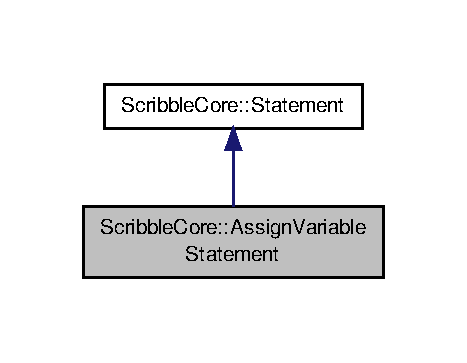
\includegraphics[width=224pt]{class_scribble_core_1_1_assign_variable_statement__inherit__graph}
\end{center}
\end{figure}


Collaboration diagram for Scribble\-Core\-:\-:Assign\-Variable\-Statement\-:\nopagebreak
\begin{figure}[H]
\begin{center}
\leavevmode
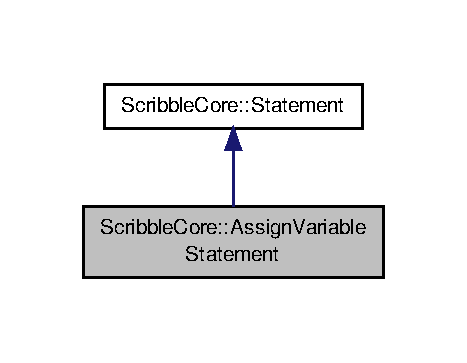
\includegraphics[width=224pt]{class_scribble_core_1_1_assign_variable_statement__coll__graph}
\end{center}
\end{figure}
\subsection*{Public Member Functions}
\begin{DoxyCompactItemize}
\item 
\hyperlink{class_scribble_core_1_1_assign_variable_statement_a4409d9bc843516435a02a9ce55041346}{Assign\-Variable\-Statement} (int line\-No, std\-::string sym, Smart\-Pointer$<$ \hyperlink{class_scribble_core_1_1_variable}{Variable} $>$ var, Safe\-Statement exp)
\item 
\hyperlink{class_scribble_core_1_1_type}{Type} $\ast$ \hyperlink{class_scribble_core_1_1_assign_variable_statement_a809f7220af1536d0912a68e6880e5c81}{type} ()
\item 
\hypertarget{class_scribble_core_1_1_assign_variable_statement_a9ad4d49c7f0691aad680cb30711cd149}{void {\bfseries check\-Tree} (\hyperlink{class_scribble_core_1_1_type}{Type} $\ast$function\-Type)}\label{class_scribble_core_1_1_assign_variable_statement_a9ad4d49c7f0691aad680cb30711cd149}

\item 
\hypertarget{class_scribble_core_1_1_assign_variable_statement_a2cd7a3d55227d0feaf7b622c02b521cb}{int {\bfseries generate\-Code} (int result\-Register, std\-::stringstream \&generated)}\label{class_scribble_core_1_1_assign_variable_statement_a2cd7a3d55227d0feaf7b622c02b521cb}

\end{DoxyCompactItemize}


\subsection{Detailed Description}
Set the value of a given variable to the result of the given statement and also return it. ( So sys.\-Write(A \-:= \char`\"{}\-Hello\char`\"{}); is valid ) 

\subsection{Constructor \& Destructor Documentation}
\hypertarget{class_scribble_core_1_1_assign_variable_statement_a4409d9bc843516435a02a9ce55041346}{\index{Scribble\-Core\-::\-Assign\-Variable\-Statement@{Scribble\-Core\-::\-Assign\-Variable\-Statement}!Assign\-Variable\-Statement@{Assign\-Variable\-Statement}}
\index{Assign\-Variable\-Statement@{Assign\-Variable\-Statement}!ScribbleCore::AssignVariableStatement@{Scribble\-Core\-::\-Assign\-Variable\-Statement}}
\subsubsection[{Assign\-Variable\-Statement}]{\setlength{\rightskip}{0pt plus 5cm}Scribble\-Core\-::\-Assign\-Variable\-Statement\-::\-Assign\-Variable\-Statement (
\begin{DoxyParamCaption}
\item[{int}]{line\-No, }
\item[{std\-::string}]{sym, }
\item[{Smart\-Pointer$<$ {\bf Variable} $>$}]{var, }
\item[{Safe\-Statement}]{exp}
\end{DoxyParamCaption}
)}}\label{class_scribble_core_1_1_assign_variable_statement_a4409d9bc843516435a02a9ce55041346}
Construct a \hyperlink{class_scribble_core_1_1_assign_variable_statement}{Assign\-Variable\-Statement}. 
\begin{DoxyParams}{Parameters}
{\em line\-No} & the line number which this occurs on. \\
\hline
{\em sym} & The symbol this was constructed from. \\
\hline
{\em var} & The variable to modify \\
\hline
{\em exp} & The expression which the variable is set to the result of. \\
\hline
\end{DoxyParams}


\subsection{Member Function Documentation}
\hypertarget{class_scribble_core_1_1_assign_variable_statement_a809f7220af1536d0912a68e6880e5c81}{\index{Scribble\-Core\-::\-Assign\-Variable\-Statement@{Scribble\-Core\-::\-Assign\-Variable\-Statement}!type@{type}}
\index{type@{type}!ScribbleCore::AssignVariableStatement@{Scribble\-Core\-::\-Assign\-Variable\-Statement}}
\subsubsection[{type}]{\setlength{\rightskip}{0pt plus 5cm}{\bf Type}$\ast$ Scribble\-Core\-::\-Assign\-Variable\-Statement\-::type (
\begin{DoxyParamCaption}
{}
\end{DoxyParamCaption}
)\hspace{0.3cm}{\ttfamily [inline]}, {\ttfamily [virtual]}}}\label{class_scribble_core_1_1_assign_variable_statement_a809f7220af1536d0912a68e6880e5c81}
Returns the type of the variable. \begin{DoxyReturn}{Returns}
The type of the variable/expression. 
\end{DoxyReturn}


Implements \hyperlink{class_scribble_core_1_1_statement}{Scribble\-Core\-::\-Statement}.



The documentation for this class was generated from the following files\-:\begin{DoxyCompactItemize}
\item 
/home/blake/\-Dropbox/\-Current/\-Scribble/src/\-Scribble/\-Statement/Assign\-Variable.\-hpp\item 
/home/blake/\-Dropbox/\-Current/\-Scribble/src/\-Scribble/\-Statement/Assign\-Variable.\-cpp\end{DoxyCompactItemize}

\hypertarget{class_scribble_core_1_1_bool_statement}{\section{Scribble\-Core\-:\-:Bool\-Statement Class Reference}
\label{class_scribble_core_1_1_bool_statement}\index{Scribble\-Core\-::\-Bool\-Statement@{Scribble\-Core\-::\-Bool\-Statement}}
}


{\ttfamily \#include $<$Bool\-Statement.\-hpp$>$}



Inheritance diagram for Scribble\-Core\-:\-:Bool\-Statement\-:
\nopagebreak
\begin{figure}[H]
\begin{center}
\leavevmode
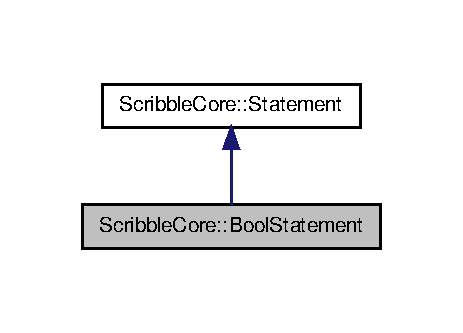
\includegraphics[width=226pt]{class_scribble_core_1_1_bool_statement__inherit__graph}
\end{center}
\end{figure}


Collaboration diagram for Scribble\-Core\-:\-:Bool\-Statement\-:
\nopagebreak
\begin{figure}[H]
\begin{center}
\leavevmode
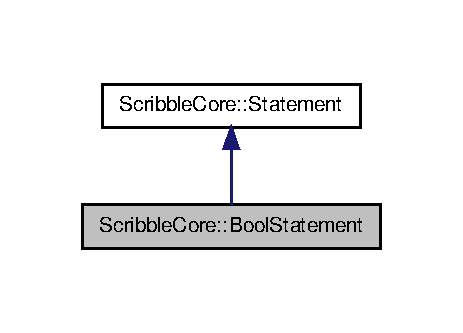
\includegraphics[width=226pt]{class_scribble_core_1_1_bool_statement__coll__graph}
\end{center}
\end{figure}
\subsection*{Public Member Functions}
\begin{DoxyCompactItemize}
\item 
\hyperlink{class_scribble_core_1_1_bool_statement_a0efd34bd9ef8bb593a1e61edf65e8357}{Bool\-Statement} (int line\-No, std\-::string sym, bool value)
\item 
virtual \hyperlink{class_scribble_core_1_1_bool_statement_a293f759a61c6ac9dd92c29d8747e048d}{$\sim$\-Bool\-Statement} ()
\item 
\hyperlink{class_scribble_core_1_1_type}{Type} $\ast$ \hyperlink{class_scribble_core_1_1_bool_statement_a9043d79db97bea428df58818d8e6de38}{type} ()
\item 
void \hyperlink{class_scribble_core_1_1_bool_statement_a7992602b1bb4a27ccb588c0d643a159f}{check\-Tree} (\hyperlink{class_scribble_core_1_1_type}{Type} $\ast$function\-Type)
\item 
virtual int \hyperlink{class_scribble_core_1_1_bool_statement_a776c4acf8cc4c0e4b0a0228df85a1fe8}{generate\-Code} (int result\-Register, std\-::stringstream \&generated)
\end{DoxyCompactItemize}


\subsection{Detailed Description}
Returns a boolean value. 

Definition at line 18 of file Bool\-Statement.\-hpp.



\subsection{Constructor \& Destructor Documentation}
\hypertarget{class_scribble_core_1_1_bool_statement_a0efd34bd9ef8bb593a1e61edf65e8357}{\index{Scribble\-Core\-::\-Bool\-Statement@{Scribble\-Core\-::\-Bool\-Statement}!Bool\-Statement@{Bool\-Statement}}
\index{Bool\-Statement@{Bool\-Statement}!ScribbleCore::BoolStatement@{Scribble\-Core\-::\-Bool\-Statement}}
\subsubsection[{Bool\-Statement}]{\setlength{\rightskip}{0pt plus 5cm}Scribble\-Core\-::\-Bool\-Statement\-::\-Bool\-Statement (
\begin{DoxyParamCaption}
\item[{int}]{line\-No, }
\item[{std\-::string}]{sym, }
\item[{bool}]{value}
\end{DoxyParamCaption}
)}}\label{class_scribble_core_1_1_bool_statement_a0efd34bd9ef8bb593a1e61edf65e8357}
Create a Bool statement 
\begin{DoxyParams}{Parameters}
{\em value} & The value to set the boolean to. \\
\hline
\end{DoxyParams}


Definition at line 14 of file Bool\-Statement.\-cpp.

\hypertarget{class_scribble_core_1_1_bool_statement_a293f759a61c6ac9dd92c29d8747e048d}{\index{Scribble\-Core\-::\-Bool\-Statement@{Scribble\-Core\-::\-Bool\-Statement}!$\sim$\-Bool\-Statement@{$\sim$\-Bool\-Statement}}
\index{$\sim$\-Bool\-Statement@{$\sim$\-Bool\-Statement}!ScribbleCore::BoolStatement@{Scribble\-Core\-::\-Bool\-Statement}}
\subsubsection[{$\sim$\-Bool\-Statement}]{\setlength{\rightskip}{0pt plus 5cm}Scribble\-Core\-::\-Bool\-Statement\-::$\sim$\-Bool\-Statement (
\begin{DoxyParamCaption}
{}
\end{DoxyParamCaption}
)\hspace{0.3cm}{\ttfamily [virtual]}}}\label{class_scribble_core_1_1_bool_statement_a293f759a61c6ac9dd92c29d8747e048d}


Definition at line 19 of file Bool\-Statement.\-cpp.



\subsection{Member Function Documentation}
\hypertarget{class_scribble_core_1_1_bool_statement_a7992602b1bb4a27ccb588c0d643a159f}{\index{Scribble\-Core\-::\-Bool\-Statement@{Scribble\-Core\-::\-Bool\-Statement}!check\-Tree@{check\-Tree}}
\index{check\-Tree@{check\-Tree}!ScribbleCore::BoolStatement@{Scribble\-Core\-::\-Bool\-Statement}}
\subsubsection[{check\-Tree}]{\setlength{\rightskip}{0pt plus 5cm}void Scribble\-Core\-::\-Bool\-Statement\-::check\-Tree (
\begin{DoxyParamCaption}
\item[{{\bf Type} $\ast$}]{function\-Type}
\end{DoxyParamCaption}
)\hspace{0.3cm}{\ttfamily [virtual]}}}\label{class_scribble_core_1_1_bool_statement_a7992602b1bb4a27ccb588c0d643a159f}


Implements \hyperlink{class_scribble_core_1_1_statement_a894e4f8d8b35279bb9ea87f20afdb978}{Scribble\-Core\-::\-Statement}.



Definition at line 26 of file Bool\-Statement.\-cpp.

\hypertarget{class_scribble_core_1_1_bool_statement_a776c4acf8cc4c0e4b0a0228df85a1fe8}{\index{Scribble\-Core\-::\-Bool\-Statement@{Scribble\-Core\-::\-Bool\-Statement}!generate\-Code@{generate\-Code}}
\index{generate\-Code@{generate\-Code}!ScribbleCore::BoolStatement@{Scribble\-Core\-::\-Bool\-Statement}}
\subsubsection[{generate\-Code}]{\setlength{\rightskip}{0pt plus 5cm}int Scribble\-Core\-::\-Bool\-Statement\-::generate\-Code (
\begin{DoxyParamCaption}
\item[{int}]{result\-Register, }
\item[{std\-::stringstream \&}]{generated}
\end{DoxyParamCaption}
)\hspace{0.3cm}{\ttfamily [virtual]}}}\label{class_scribble_core_1_1_bool_statement_a776c4acf8cc4c0e4b0a0228df85a1fe8}


Reimplemented from \hyperlink{class_scribble_core_1_1_statement_aa3951ffef06ca195054a0bdfc8a4c8de}{Scribble\-Core\-::\-Statement}.



Definition at line 29 of file Bool\-Statement.\-cpp.

\hypertarget{class_scribble_core_1_1_bool_statement_a9043d79db97bea428df58818d8e6de38}{\index{Scribble\-Core\-::\-Bool\-Statement@{Scribble\-Core\-::\-Bool\-Statement}!type@{type}}
\index{type@{type}!ScribbleCore::BoolStatement@{Scribble\-Core\-::\-Bool\-Statement}}
\subsubsection[{type}]{\setlength{\rightskip}{0pt plus 5cm}{\bf Type} $\ast$ Scribble\-Core\-::\-Bool\-Statement\-::type (
\begin{DoxyParamCaption}
{}
\end{DoxyParamCaption}
)\hspace{0.3cm}{\ttfamily [virtual]}}}\label{class_scribble_core_1_1_bool_statement_a9043d79db97bea428df58818d8e6de38}
Returns a boolean \begin{DoxyReturn}{Returns}
Boolean 
\end{DoxyReturn}


Implements \hyperlink{class_scribble_core_1_1_statement_a532ed5a44ec49873dc191dae7ddc8b00}{Scribble\-Core\-::\-Statement}.



Definition at line 22 of file Bool\-Statement.\-cpp.



Here is the call graph for this function\-:
\nopagebreak
\begin{figure}[H]
\begin{center}
\leavevmode
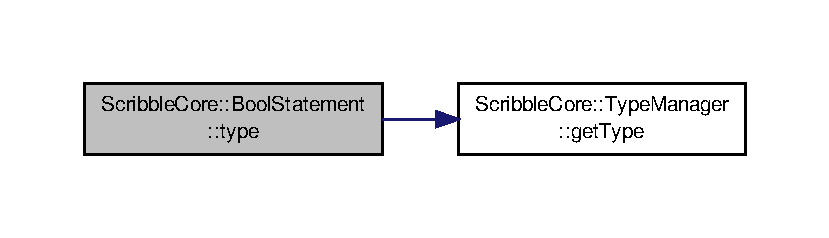
\includegraphics[width=350pt]{class_scribble_core_1_1_bool_statement_a9043d79db97bea428df58818d8e6de38_cgraph}
\end{center}
\end{figure}




The documentation for this class was generated from the following files\-:\begin{DoxyCompactItemize}
\item 
/home/blake/\-Dropbox/\-Current/\-Scribble/src/\-Scribble/\-Statement/\hyperlink{_bool_statement_8hpp}{Bool\-Statement.\-hpp}\item 
/home/blake/\-Dropbox/\-Current/\-Scribble/src/\-Scribble/\-Statement/\hyperlink{_bool_statement_8cpp}{Bool\-Statement.\-cpp}\end{DoxyCompactItemize}

\hypertarget{class_bool_to_string_function}{\section{Bool\-To\-String\-Function Class Reference}
\label{class_bool_to_string_function}\index{Bool\-To\-String\-Function@{Bool\-To\-String\-Function}}
}


{\ttfamily \#include $<$String\-Function.\-hpp$>$}



Inheritance diagram for Bool\-To\-String\-Function\-:
\nopagebreak
\begin{figure}[H]
\begin{center}
\leavevmode
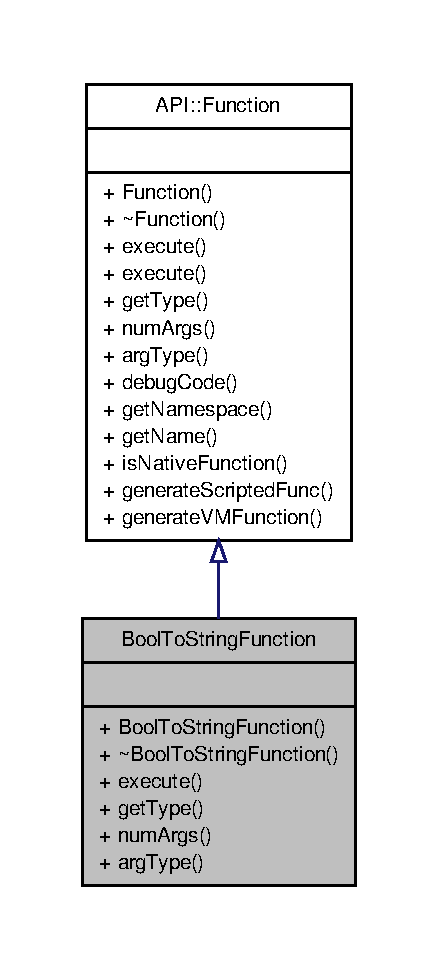
\includegraphics[width=210pt]{class_bool_to_string_function__inherit__graph}
\end{center}
\end{figure}


Collaboration diagram for Bool\-To\-String\-Function\-:
\nopagebreak
\begin{figure}[H]
\begin{center}
\leavevmode
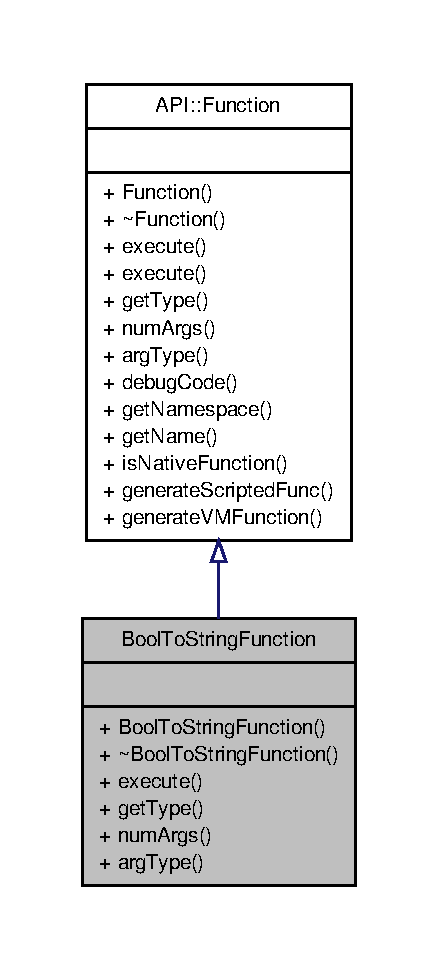
\includegraphics[width=210pt]{class_bool_to_string_function__coll__graph}
\end{center}
\end{figure}
\subsection*{Public Member Functions}
\begin{DoxyCompactItemize}
\item 
\hyperlink{class_bool_to_string_function_a9a8da1c0053f40bd06eb3c8a9e243631}{Bool\-To\-String\-Function} (std\-::string ns)
\item 
virtual \hyperlink{class_bool_to_string_function_a2b75b41ac8e41de00ebc770fb62d264b}{$\sim$\-Bool\-To\-String\-Function} ()
\item 
virtual \hyperlink{class_a_p_i_1_1_a_p_i_value}{A\-P\-I\-::\-A\-P\-I\-Value} \hyperlink{class_bool_to_string_function_a4e74a7af474a601db96557e9ff5caffe}{execute} (\hyperlink{class_a_p_i_1_1_a_p_i_value}{A\-P\-I\-::\-A\-P\-I\-Value} $\ast$values, \hyperlink{class_v_m_1_1_virtual_machine}{V\-M\-::\-Virtual\-Machine} $\ast$virt)
\item 
\hyperlink{class_scribble_core_1_1_type}{Scribble\-Core\-::\-Type} $\ast$ \hyperlink{class_bool_to_string_function_a3372750cab22e2ebebde6f1cd4ad3159}{get\-Type} ()
\item 
const unsigned int \hyperlink{class_bool_to_string_function_a82bdbb122bdaa5046158981dfc5211aa}{num\-Args} ()
\item 
\hyperlink{class_scribble_core_1_1_type}{Scribble\-Core\-::\-Type} $\ast$ \hyperlink{class_bool_to_string_function_affe0b7e270045bfa7fdbd7fa65c9174b}{arg\-Type} (unsigned int arg)
\end{DoxyCompactItemize}
\subsection*{Additional Inherited Members}


\subsection{Detailed Description}


Definition at line 41 of file String\-Function.\-hpp.



\subsection{Constructor \& Destructor Documentation}
\hypertarget{class_bool_to_string_function_a9a8da1c0053f40bd06eb3c8a9e243631}{\index{Bool\-To\-String\-Function@{Bool\-To\-String\-Function}!Bool\-To\-String\-Function@{Bool\-To\-String\-Function}}
\index{Bool\-To\-String\-Function@{Bool\-To\-String\-Function}!BoolToStringFunction@{Bool\-To\-String\-Function}}
\subsubsection[{Bool\-To\-String\-Function}]{\setlength{\rightskip}{0pt plus 5cm}Bool\-To\-String\-Function\-::\-Bool\-To\-String\-Function (
\begin{DoxyParamCaption}
\item[{std\-::string}]{ns}
\end{DoxyParamCaption}
)}}\label{class_bool_to_string_function_a9a8da1c0053f40bd06eb3c8a9e243631}


Definition at line 56 of file String\-Function.\-cpp.

\hypertarget{class_bool_to_string_function_a2b75b41ac8e41de00ebc770fb62d264b}{\index{Bool\-To\-String\-Function@{Bool\-To\-String\-Function}!$\sim$\-Bool\-To\-String\-Function@{$\sim$\-Bool\-To\-String\-Function}}
\index{$\sim$\-Bool\-To\-String\-Function@{$\sim$\-Bool\-To\-String\-Function}!BoolToStringFunction@{Bool\-To\-String\-Function}}
\subsubsection[{$\sim$\-Bool\-To\-String\-Function}]{\setlength{\rightskip}{0pt plus 5cm}Bool\-To\-String\-Function\-::$\sim$\-Bool\-To\-String\-Function (
\begin{DoxyParamCaption}
{}
\end{DoxyParamCaption}
)\hspace{0.3cm}{\ttfamily [virtual]}}}\label{class_bool_to_string_function_a2b75b41ac8e41de00ebc770fb62d264b}


Definition at line 62 of file String\-Function.\-cpp.



\subsection{Member Function Documentation}
\hypertarget{class_bool_to_string_function_affe0b7e270045bfa7fdbd7fa65c9174b}{\index{Bool\-To\-String\-Function@{Bool\-To\-String\-Function}!arg\-Type@{arg\-Type}}
\index{arg\-Type@{arg\-Type}!BoolToStringFunction@{Bool\-To\-String\-Function}}
\subsubsection[{arg\-Type}]{\setlength{\rightskip}{0pt plus 5cm}{\bf Scribble\-Core\-::\-Type} $\ast$ Bool\-To\-String\-Function\-::arg\-Type (
\begin{DoxyParamCaption}
\item[{unsigned int}]{arg}
\end{DoxyParamCaption}
)\hspace{0.3cm}{\ttfamily [virtual]}}}\label{class_bool_to_string_function_affe0b7e270045bfa7fdbd7fa65c9174b}
Get the expected type of the specified argument 

Implements \hyperlink{class_a_p_i_1_1_function_a531806ea8476e8aa396eb98ce81e713b}{A\-P\-I\-::\-Function}.



Definition at line 74 of file String\-Function.\-cpp.



Here is the call graph for this function\-:
\nopagebreak
\begin{figure}[H]
\begin{center}
\leavevmode
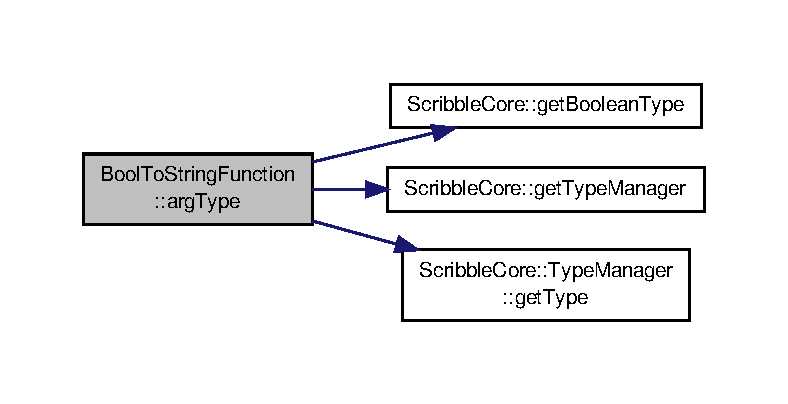
\includegraphics[width=350pt]{class_bool_to_string_function_affe0b7e270045bfa7fdbd7fa65c9174b_cgraph}
\end{center}
\end{figure}


\hypertarget{class_bool_to_string_function_a4e74a7af474a601db96557e9ff5caffe}{\index{Bool\-To\-String\-Function@{Bool\-To\-String\-Function}!execute@{execute}}
\index{execute@{execute}!BoolToStringFunction@{Bool\-To\-String\-Function}}
\subsubsection[{execute}]{\setlength{\rightskip}{0pt plus 5cm}{\bf A\-P\-I\-::\-A\-P\-I\-Value} Bool\-To\-String\-Function\-::execute (
\begin{DoxyParamCaption}
\item[{{\bf A\-P\-I\-::\-A\-P\-I\-Value} $\ast$}]{values, }
\item[{{\bf V\-M\-::\-Virtual\-Machine} $\ast$}]{virt}
\end{DoxyParamCaption}
)\hspace{0.3cm}{\ttfamily [virtual]}}}\label{class_bool_to_string_function_a4e74a7af474a601db96557e9ff5caffe}
This function executes the given \hyperlink{class_a_p_i_1_1_function}{A\-P\-I\-::\-Function} and returns it's result. It called by the more complex \hyperlink{class_a_p_i_1_1_function_a5acc2022cdbd5fe47c1a04769a1d8cf4}{execute(\-V\-M\-::\-Virtual\-Machine$\ast$)} after that function has converted all arguments into \hyperlink{namespace_a_p_i}{A\-P\-I} values. 
\begin{DoxyParams}{Parameters}
{\em args} & The arguments passed to the function \\
\hline
{\em virt} & The virtual machine this function is being run in the context of. \\
\hline
\end{DoxyParams}
\begin{DoxyReturn}{Returns}
The resulting \hyperlink{namespace_a_p_i}{A\-P\-I} value 
\end{DoxyReturn}


Reimplemented from \hyperlink{class_a_p_i_1_1_function_ac3bc5de6ce095a4c8474525ef181c4af}{A\-P\-I\-::\-Function}.



Definition at line 83 of file String\-Function.\-cpp.



Here is the call graph for this function\-:
\nopagebreak
\begin{figure}[H]
\begin{center}
\leavevmode
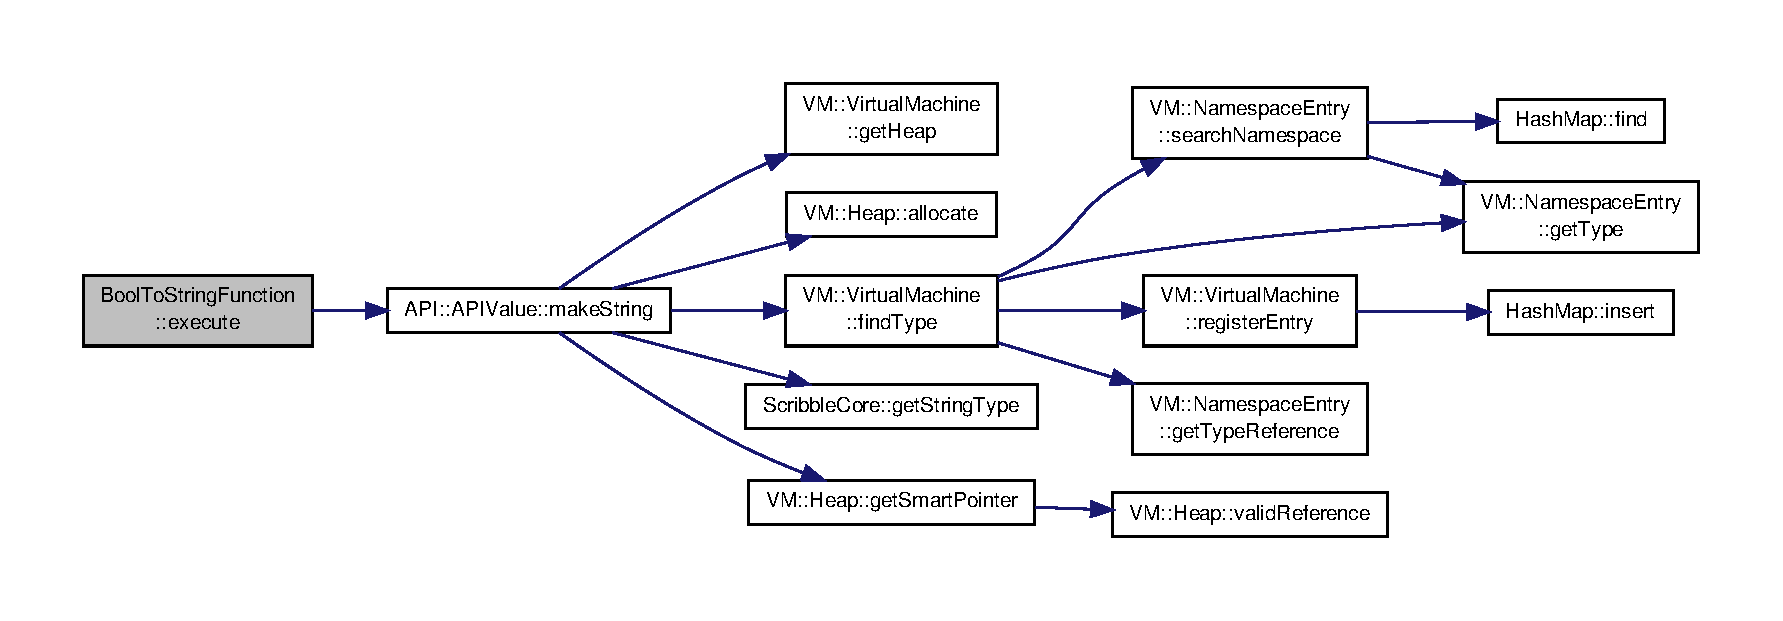
\includegraphics[width=350pt]{class_bool_to_string_function_a4e74a7af474a601db96557e9ff5caffe_cgraph}
\end{center}
\end{figure}


\hypertarget{class_bool_to_string_function_a3372750cab22e2ebebde6f1cd4ad3159}{\index{Bool\-To\-String\-Function@{Bool\-To\-String\-Function}!get\-Type@{get\-Type}}
\index{get\-Type@{get\-Type}!BoolToStringFunction@{Bool\-To\-String\-Function}}
\subsubsection[{get\-Type}]{\setlength{\rightskip}{0pt plus 5cm}{\bf Scribble\-Core\-::\-Type} $\ast$ Bool\-To\-String\-Function\-::get\-Type (
\begin{DoxyParamCaption}
{}
\end{DoxyParamCaption}
)\hspace{0.3cm}{\ttfamily [virtual]}}}\label{class_bool_to_string_function_a3372750cab22e2ebebde6f1cd4ad3159}
Get the return type of the function 

Implements \hyperlink{class_a_p_i_1_1_function_a85b0b2ee88d3ac61a0e77f94e06445b1}{A\-P\-I\-::\-Function}.



Definition at line 66 of file String\-Function.\-cpp.



Here is the call graph for this function\-:
\nopagebreak
\begin{figure}[H]
\begin{center}
\leavevmode
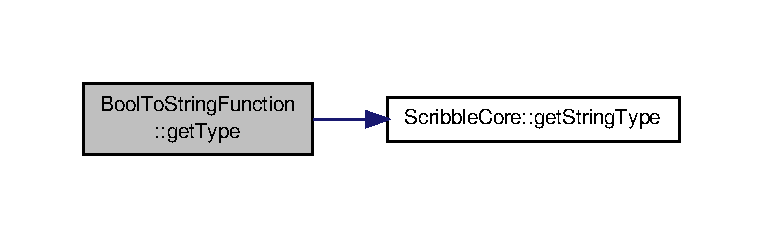
\includegraphics[width=350pt]{class_bool_to_string_function_a3372750cab22e2ebebde6f1cd4ad3159_cgraph}
\end{center}
\end{figure}


\hypertarget{class_bool_to_string_function_a82bdbb122bdaa5046158981dfc5211aa}{\index{Bool\-To\-String\-Function@{Bool\-To\-String\-Function}!num\-Args@{num\-Args}}
\index{num\-Args@{num\-Args}!BoolToStringFunction@{Bool\-To\-String\-Function}}
\subsubsection[{num\-Args}]{\setlength{\rightskip}{0pt plus 5cm}unsigned int const Bool\-To\-String\-Function\-::num\-Args (
\begin{DoxyParamCaption}
{}
\end{DoxyParamCaption}
)\hspace{0.3cm}{\ttfamily [virtual]}}}\label{class_bool_to_string_function_a82bdbb122bdaa5046158981dfc5211aa}
Return the number of arguments the function takes 

Implements \hyperlink{class_a_p_i_1_1_function_ae56761ad4c849c05e12cb4cd02583c77}{A\-P\-I\-::\-Function}.



Definition at line 70 of file String\-Function.\-cpp.



The documentation for this class was generated from the following files\-:\begin{DoxyCompactItemize}
\item 
/home/blake/\-Dropbox/\-Current/\-Scribble/src/\-A\-P\-I/\hyperlink{_string_function_8hpp}{String\-Function.\-hpp}\item 
/home/blake/\-Dropbox/\-Current/\-Scribble/src/\-A\-P\-I/\hyperlink{_string_function_8cpp}{String\-Function.\-cpp}\end{DoxyCompactItemize}

\hypertarget{class_a_p_i_1_1_concat}{\section{A\-P\-I\-:\-:Concat Class Reference}
\label{class_a_p_i_1_1_concat}\index{A\-P\-I\-::\-Concat@{A\-P\-I\-::\-Concat}}
}


Inheritance diagram for A\-P\-I\-:\-:Concat\-:\nopagebreak
\begin{figure}[H]
\begin{center}
\leavevmode
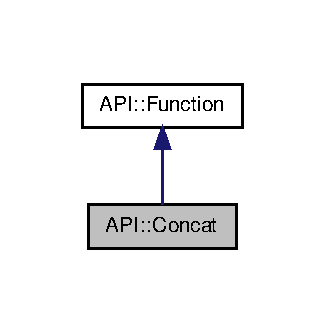
\includegraphics[width=156pt]{class_a_p_i_1_1_concat__inherit__graph}
\end{center}
\end{figure}


Collaboration diagram for A\-P\-I\-:\-:Concat\-:\nopagebreak
\begin{figure}[H]
\begin{center}
\leavevmode
\includegraphics[width=156pt]{class_a_p_i_1_1_concat__coll__graph}
\end{center}
\end{figure}
\subsection*{Public Member Functions}
\begin{DoxyCompactItemize}
\item 
\hypertarget{class_a_p_i_1_1_concat_a370aba5db6157a49783a5d8e09c4690c}{{\bfseries Concat} (std\-::string ns)}\label{class_a_p_i_1_1_concat_a370aba5db6157a49783a5d8e09c4690c}

\item 
\hyperlink{class_a_p_i_1_1_a_p_i_value}{A\-P\-I\-::\-A\-P\-I\-Value} \hyperlink{class_a_p_i_1_1_concat_a8dbf36574a9a16077bff5bfd634669fd}{execute} (\hyperlink{class_a_p_i_1_1_a_p_i_value}{A\-P\-I\-::\-A\-P\-I\-Value} $\ast$values, \hyperlink{class_v_m_1_1_virtual_machine}{V\-M\-::\-Virtual\-Machine} $\ast$virt)
\item 
virtual \hyperlink{class_scribble_core_1_1_type}{Scribble\-Core\-::\-Type} $\ast$ \hyperlink{class_a_p_i_1_1_concat_a68ea98c2d699faf3313def2dbd453740}{get\-Type} ()
\item 
virtual const unsigned int \hyperlink{class_a_p_i_1_1_concat_ae88cb6c929ad4b639d0b156129ac1942}{num\-Args} ()
\item 
virtual \hyperlink{class_scribble_core_1_1_type}{Scribble\-Core\-::\-Type} $\ast$ \hyperlink{class_a_p_i_1_1_concat_a81a12d248a79a10df234b898d0ee1c7f}{arg\-Type} (unsigned int arg)
\end{DoxyCompactItemize}
\subsection*{Additional Inherited Members}


\subsection{Member Function Documentation}
\hypertarget{class_a_p_i_1_1_concat_a81a12d248a79a10df234b898d0ee1c7f}{\index{A\-P\-I\-::\-Concat@{A\-P\-I\-::\-Concat}!arg\-Type@{arg\-Type}}
\index{arg\-Type@{arg\-Type}!API::Concat@{A\-P\-I\-::\-Concat}}
\subsubsection[{arg\-Type}]{\setlength{\rightskip}{0pt plus 5cm}{\bf Scribble\-Core\-::\-Type} $\ast$ A\-P\-I\-::\-Concat\-::arg\-Type (
\begin{DoxyParamCaption}
\item[{unsigned int}]{arg}
\end{DoxyParamCaption}
)\hspace{0.3cm}{\ttfamily [virtual]}}}\label{class_a_p_i_1_1_concat_a81a12d248a79a10df234b898d0ee1c7f}
Get the expected type of the specified argument 

Implements \hyperlink{class_a_p_i_1_1_function_a531806ea8476e8aa396eb98ce81e713b}{A\-P\-I\-::\-Function}.



Here is the call graph for this function\-:
\nopagebreak
\begin{figure}[H]
\begin{center}
\leavevmode
\includegraphics[width=350pt]{class_a_p_i_1_1_concat_a81a12d248a79a10df234b898d0ee1c7f_cgraph}
\end{center}
\end{figure}


\hypertarget{class_a_p_i_1_1_concat_a8dbf36574a9a16077bff5bfd634669fd}{\index{A\-P\-I\-::\-Concat@{A\-P\-I\-::\-Concat}!execute@{execute}}
\index{execute@{execute}!API::Concat@{A\-P\-I\-::\-Concat}}
\subsubsection[{execute}]{\setlength{\rightskip}{0pt plus 5cm}{\bf A\-P\-I\-::\-A\-P\-I\-Value} A\-P\-I\-::\-Concat\-::execute (
\begin{DoxyParamCaption}
\item[{{\bf A\-P\-I\-::\-A\-P\-I\-Value} $\ast$}]{values, }
\item[{{\bf V\-M\-::\-Virtual\-Machine} $\ast$}]{virt}
\end{DoxyParamCaption}
)\hspace{0.3cm}{\ttfamily [virtual]}}}\label{class_a_p_i_1_1_concat_a8dbf36574a9a16077bff5bfd634669fd}
This function executes the given \hyperlink{class_a_p_i_1_1_function}{A\-P\-I\-::\-Function} and returns it's result. It called by the more complex execute(\-V\-M\-::\-Virtual\-Machine$\ast$) after that function has converted all arguments into \hyperlink{namespace_a_p_i}{A\-P\-I} values. 
\begin{DoxyParams}{Parameters}
{\em args} & The arguments passed to the function \\
\hline
{\em virt} & The virtual machine this function is being run in the context of. \\
\hline
\end{DoxyParams}
\begin{DoxyReturn}{Returns}
The resulting \hyperlink{namespace_a_p_i}{A\-P\-I} value 
\end{DoxyReturn}


Reimplemented from \hyperlink{class_a_p_i_1_1_function_ac3bc5de6ce095a4c8474525ef181c4af}{A\-P\-I\-::\-Function}.



Here is the call graph for this function\-:\nopagebreak
\begin{figure}[H]
\begin{center}
\leavevmode
\includegraphics[width=350pt]{class_a_p_i_1_1_concat_a8dbf36574a9a16077bff5bfd634669fd_cgraph}
\end{center}
\end{figure}


\hypertarget{class_a_p_i_1_1_concat_a68ea98c2d699faf3313def2dbd453740}{\index{A\-P\-I\-::\-Concat@{A\-P\-I\-::\-Concat}!get\-Type@{get\-Type}}
\index{get\-Type@{get\-Type}!API::Concat@{A\-P\-I\-::\-Concat}}
\subsubsection[{get\-Type}]{\setlength{\rightskip}{0pt plus 5cm}{\bf Scribble\-Core\-::\-Type} $\ast$ A\-P\-I\-::\-Concat\-::get\-Type (
\begin{DoxyParamCaption}
{}
\end{DoxyParamCaption}
)\hspace{0.3cm}{\ttfamily [virtual]}}}\label{class_a_p_i_1_1_concat_a68ea98c2d699faf3313def2dbd453740}
Get the return type of the function 

Implements \hyperlink{class_a_p_i_1_1_function_a85b0b2ee88d3ac61a0e77f94e06445b1}{A\-P\-I\-::\-Function}.



Here is the call graph for this function\-:
\nopagebreak
\begin{figure}[H]
\begin{center}
\leavevmode
\includegraphics[width=350pt]{class_a_p_i_1_1_concat_a68ea98c2d699faf3313def2dbd453740_cgraph}
\end{center}
\end{figure}


\hypertarget{class_a_p_i_1_1_concat_ae88cb6c929ad4b639d0b156129ac1942}{\index{A\-P\-I\-::\-Concat@{A\-P\-I\-::\-Concat}!num\-Args@{num\-Args}}
\index{num\-Args@{num\-Args}!API::Concat@{A\-P\-I\-::\-Concat}}
\subsubsection[{num\-Args}]{\setlength{\rightskip}{0pt plus 5cm}const unsigned int A\-P\-I\-::\-Concat\-::num\-Args (
\begin{DoxyParamCaption}
{}
\end{DoxyParamCaption}
)\hspace{0.3cm}{\ttfamily [virtual]}}}\label{class_a_p_i_1_1_concat_ae88cb6c929ad4b639d0b156129ac1942}
Return the number of arguments the function takes 

Implements \hyperlink{class_a_p_i_1_1_function_ae56761ad4c849c05e12cb4cd02583c77}{A\-P\-I\-::\-Function}.



The documentation for this class was generated from the following files\-:\begin{DoxyCompactItemize}
\item 
/home/blake/\-Dropbox/\-Current/\-Scribble/src/\-A\-P\-I/Concat.\-hpp\item 
/home/blake/\-Dropbox/\-Current/\-Scribble/src/\-A\-P\-I/Concat.\-cpp\end{DoxyCompactItemize}

\hypertarget{class_a_p_i_1_1_fatal_error}{\section{A\-P\-I\-:\-:Fatal\-Error Class Reference}
\label{class_a_p_i_1_1_fatal_error}\index{A\-P\-I\-::\-Fatal\-Error@{A\-P\-I\-::\-Fatal\-Error}}
}


{\ttfamily \#include $<$Fatal\-Error.\-hpp$>$}



Collaboration diagram for A\-P\-I\-:\-:Fatal\-Error\-:
\nopagebreak
\begin{figure}[H]
\begin{center}
\leavevmode
\includegraphics[width=162pt]{class_a_p_i_1_1_fatal_error__coll__graph}
\end{center}
\end{figure}
\subsection*{Public Member Functions}
\begin{DoxyCompactItemize}
\item 
\hyperlink{class_a_p_i_1_1_fatal_error_a32634cedeb45f77bbdc11a8eb0946414}{Fatal\-Error} ()
\item 
virtual \hyperlink{class_a_p_i_1_1_fatal_error_a42da2d68aec87f57c8bbcfe0302ae3da}{$\sim$\-Fatal\-Error} ()
\end{DoxyCompactItemize}


\subsection{Detailed Description}


Definition at line 13 of file Fatal\-Error.\-hpp.



\subsection{Constructor \& Destructor Documentation}
\hypertarget{class_a_p_i_1_1_fatal_error_a32634cedeb45f77bbdc11a8eb0946414}{\index{A\-P\-I\-::\-Fatal\-Error@{A\-P\-I\-::\-Fatal\-Error}!Fatal\-Error@{Fatal\-Error}}
\index{Fatal\-Error@{Fatal\-Error}!API::FatalError@{A\-P\-I\-::\-Fatal\-Error}}
\subsubsection[{Fatal\-Error}]{\setlength{\rightskip}{0pt plus 5cm}A\-P\-I\-::\-Fatal\-Error\-::\-Fatal\-Error (
\begin{DoxyParamCaption}
{}
\end{DoxyParamCaption}
)}}\label{class_a_p_i_1_1_fatal_error_a32634cedeb45f77bbdc11a8eb0946414}


Definition at line 12 of file Fatal\-Error.\-cpp.

\hypertarget{class_a_p_i_1_1_fatal_error_a42da2d68aec87f57c8bbcfe0302ae3da}{\index{A\-P\-I\-::\-Fatal\-Error@{A\-P\-I\-::\-Fatal\-Error}!$\sim$\-Fatal\-Error@{$\sim$\-Fatal\-Error}}
\index{$\sim$\-Fatal\-Error@{$\sim$\-Fatal\-Error}!API::FatalError@{A\-P\-I\-::\-Fatal\-Error}}
\subsubsection[{$\sim$\-Fatal\-Error}]{\setlength{\rightskip}{0pt plus 5cm}A\-P\-I\-::\-Fatal\-Error\-::$\sim$\-Fatal\-Error (
\begin{DoxyParamCaption}
{}
\end{DoxyParamCaption}
)\hspace{0.3cm}{\ttfamily [virtual]}}}\label{class_a_p_i_1_1_fatal_error_a42da2d68aec87f57c8bbcfe0302ae3da}


Definition at line 17 of file Fatal\-Error.\-cpp.



The documentation for this class was generated from the following files\-:\begin{DoxyCompactItemize}
\item 
/home/blake/\-Dropbox/\-Current/\-Scribble/src/\-A\-P\-I/\hyperlink{_fatal_error_8hpp}{Fatal\-Error.\-hpp}\item 
/home/blake/\-Dropbox/\-Current/\-Scribble/src/\-A\-P\-I/\hyperlink{_fatal_error_8cpp}{Fatal\-Error.\-cpp}\end{DoxyCompactItemize}

\hypertarget{class_a_p_i_1_1_float32_from_int}{\section{A\-P\-I\-:\-:Float32\-From\-Int Class Reference}
\label{class_a_p_i_1_1_float32_from_int}\index{A\-P\-I\-::\-Float32\-From\-Int@{A\-P\-I\-::\-Float32\-From\-Int}}
}


Inheritance diagram for A\-P\-I\-:\-:Float32\-From\-Int\-:\nopagebreak
\begin{figure}[H]
\begin{center}
\leavevmode
\includegraphics[width=184pt]{class_a_p_i_1_1_float32_from_int__inherit__graph}
\end{center}
\end{figure}


Collaboration diagram for A\-P\-I\-:\-:Float32\-From\-Int\-:\nopagebreak
\begin{figure}[H]
\begin{center}
\leavevmode
\includegraphics[width=184pt]{class_a_p_i_1_1_float32_from_int__coll__graph}
\end{center}
\end{figure}
\subsection*{Public Member Functions}
\begin{DoxyCompactItemize}
\item 
\hypertarget{class_a_p_i_1_1_float32_from_int_a0e816789136fbf1ba91aba51ab82ef59}{{\bfseries Float32\-From\-Int} (std\-::string ns)}\label{class_a_p_i_1_1_float32_from_int_a0e816789136fbf1ba91aba51ab82ef59}

\item 
\hyperlink{class_a_p_i_1_1_a_p_i_value}{A\-P\-I\-::\-A\-P\-I\-Value} \hyperlink{class_a_p_i_1_1_float32_from_int_a945c3489f41a5f2f4e1bd3e8ffc56f21}{execute} (\hyperlink{class_a_p_i_1_1_a_p_i_value}{A\-P\-I\-::\-A\-P\-I\-Value} $\ast$values, \hyperlink{class_v_m_1_1_virtual_machine}{V\-M\-::\-Virtual\-Machine} $\ast$virt)
\item 
virtual \hyperlink{class_scribble_core_1_1_type}{Scribble\-Core\-::\-Type} $\ast$ \hyperlink{class_a_p_i_1_1_float32_from_int_a0c4ece788e44007d1099d3b18fa06889}{get\-Type} ()
\item 
virtual const unsigned int \hyperlink{class_a_p_i_1_1_float32_from_int_af54cec4109e664db95ae453e8664eaf8}{num\-Args} ()
\item 
virtual \hyperlink{class_scribble_core_1_1_type}{Scribble\-Core\-::\-Type} $\ast$ \hyperlink{class_a_p_i_1_1_float32_from_int_a0f4b92186c6091c1232612d5142fff4b}{arg\-Type} (unsigned int arg)
\end{DoxyCompactItemize}
\subsection*{Additional Inherited Members}


\subsection{Member Function Documentation}
\hypertarget{class_a_p_i_1_1_float32_from_int_a0f4b92186c6091c1232612d5142fff4b}{\index{A\-P\-I\-::\-Float32\-From\-Int@{A\-P\-I\-::\-Float32\-From\-Int}!arg\-Type@{arg\-Type}}
\index{arg\-Type@{arg\-Type}!API::Float32FromInt@{A\-P\-I\-::\-Float32\-From\-Int}}
\subsubsection[{arg\-Type}]{\setlength{\rightskip}{0pt plus 5cm}{\bf Scribble\-Core\-::\-Type} $\ast$ A\-P\-I\-::\-Float32\-From\-Int\-::arg\-Type (
\begin{DoxyParamCaption}
\item[{unsigned int}]{arg}
\end{DoxyParamCaption}
)\hspace{0.3cm}{\ttfamily [virtual]}}}\label{class_a_p_i_1_1_float32_from_int_a0f4b92186c6091c1232612d5142fff4b}
Get the expected type of the specified argument 

Implements \hyperlink{class_a_p_i_1_1_function_a531806ea8476e8aa396eb98ce81e713b}{A\-P\-I\-::\-Function}.



Here is the call graph for this function\-:\nopagebreak
\begin{figure}[H]
\begin{center}
\leavevmode
\includegraphics[width=350pt]{class_a_p_i_1_1_float32_from_int_a0f4b92186c6091c1232612d5142fff4b_cgraph}
\end{center}
\end{figure}


\hypertarget{class_a_p_i_1_1_float32_from_int_a945c3489f41a5f2f4e1bd3e8ffc56f21}{\index{A\-P\-I\-::\-Float32\-From\-Int@{A\-P\-I\-::\-Float32\-From\-Int}!execute@{execute}}
\index{execute@{execute}!API::Float32FromInt@{A\-P\-I\-::\-Float32\-From\-Int}}
\subsubsection[{execute}]{\setlength{\rightskip}{0pt plus 5cm}{\bf A\-P\-I\-::\-A\-P\-I\-Value} A\-P\-I\-::\-Float32\-From\-Int\-::execute (
\begin{DoxyParamCaption}
\item[{{\bf A\-P\-I\-::\-A\-P\-I\-Value} $\ast$}]{values, }
\item[{{\bf V\-M\-::\-Virtual\-Machine} $\ast$}]{virt}
\end{DoxyParamCaption}
)\hspace{0.3cm}{\ttfamily [virtual]}}}\label{class_a_p_i_1_1_float32_from_int_a945c3489f41a5f2f4e1bd3e8ffc56f21}
This function executes the given \hyperlink{class_a_p_i_1_1_function}{A\-P\-I\-::\-Function} and returns it's result. It called by the more complex execute(\-V\-M\-::\-Virtual\-Machine$\ast$) after that function has converted all arguments into \hyperlink{namespace_a_p_i}{A\-P\-I} values. 
\begin{DoxyParams}{Parameters}
{\em args} & The arguments passed to the function \\
\hline
{\em virt} & The virtual machine this function is being run in the context of. \\
\hline
\end{DoxyParams}
\begin{DoxyReturn}{Returns}
The resulting \hyperlink{namespace_a_p_i}{A\-P\-I} value 
\end{DoxyReturn}


Reimplemented from \hyperlink{class_a_p_i_1_1_function_ac3bc5de6ce095a4c8474525ef181c4af}{A\-P\-I\-::\-Function}.

\hypertarget{class_a_p_i_1_1_float32_from_int_a0c4ece788e44007d1099d3b18fa06889}{\index{A\-P\-I\-::\-Float32\-From\-Int@{A\-P\-I\-::\-Float32\-From\-Int}!get\-Type@{get\-Type}}
\index{get\-Type@{get\-Type}!API::Float32FromInt@{A\-P\-I\-::\-Float32\-From\-Int}}
\subsubsection[{get\-Type}]{\setlength{\rightskip}{0pt plus 5cm}{\bf Scribble\-Core\-::\-Type} $\ast$ A\-P\-I\-::\-Float32\-From\-Int\-::get\-Type (
\begin{DoxyParamCaption}
{}
\end{DoxyParamCaption}
)\hspace{0.3cm}{\ttfamily [virtual]}}}\label{class_a_p_i_1_1_float32_from_int_a0c4ece788e44007d1099d3b18fa06889}
Get the return type of the function 

Implements \hyperlink{class_a_p_i_1_1_function_a85b0b2ee88d3ac61a0e77f94e06445b1}{A\-P\-I\-::\-Function}.

\hypertarget{class_a_p_i_1_1_float32_from_int_af54cec4109e664db95ae453e8664eaf8}{\index{A\-P\-I\-::\-Float32\-From\-Int@{A\-P\-I\-::\-Float32\-From\-Int}!num\-Args@{num\-Args}}
\index{num\-Args@{num\-Args}!API::Float32FromInt@{A\-P\-I\-::\-Float32\-From\-Int}}
\subsubsection[{num\-Args}]{\setlength{\rightskip}{0pt plus 5cm}const unsigned int A\-P\-I\-::\-Float32\-From\-Int\-::num\-Args (
\begin{DoxyParamCaption}
{}
\end{DoxyParamCaption}
)\hspace{0.3cm}{\ttfamily [virtual]}}}\label{class_a_p_i_1_1_float32_from_int_af54cec4109e664db95ae453e8664eaf8}
Return the number of arguments the function takes 

Implements \hyperlink{class_a_p_i_1_1_function_ae56761ad4c849c05e12cb4cd02583c77}{A\-P\-I\-::\-Function}.



The documentation for this class was generated from the following files\-:\begin{DoxyCompactItemize}
\item 
/home/blake/\-Dropbox/\-Current/\-Scribble/src/\-A\-P\-I/Float.\-hpp\item 
/home/blake/\-Dropbox/\-Current/\-Scribble/src/\-A\-P\-I/Float.\-cpp\end{DoxyCompactItemize}

\hypertarget{class_scribble_core_1_1_float32_statement}{\section{Scribble\-Core\-:\-:Float32\-Statement Class Reference}
\label{class_scribble_core_1_1_float32_statement}\index{Scribble\-Core\-::\-Float32\-Statement@{Scribble\-Core\-::\-Float32\-Statement}}
}


Inheritance diagram for Scribble\-Core\-:\-:Float32\-Statement\-:\nopagebreak
\begin{figure}[H]
\begin{center}
\leavevmode
\includegraphics[width=236pt]{class_scribble_core_1_1_float32_statement__inherit__graph}
\end{center}
\end{figure}


Collaboration diagram for Scribble\-Core\-:\-:Float32\-Statement\-:\nopagebreak
\begin{figure}[H]
\begin{center}
\leavevmode
\includegraphics[width=236pt]{class_scribble_core_1_1_float32_statement__coll__graph}
\end{center}
\end{figure}
\subsection*{Public Member Functions}
\begin{DoxyCompactItemize}
\item 
\hypertarget{class_scribble_core_1_1_float32_statement_ab66923b22e1fb3efdac02f4f50f253ce}{{\bfseries Float32\-Statement} (int line\-No, std\-::string sym, float32\-\_\-t val)}\label{class_scribble_core_1_1_float32_statement_ab66923b22e1fb3efdac02f4f50f253ce}

\item 
\hypertarget{class_scribble_core_1_1_float32_statement_ac9a00240c3eec2c34ffdbf2d4a91e564}{\hyperlink{class_scribble_core_1_1_type}{Type} $\ast$ {\bfseries type} ()}\label{class_scribble_core_1_1_float32_statement_ac9a00240c3eec2c34ffdbf2d4a91e564}

\item 
\hypertarget{class_scribble_core_1_1_float32_statement_afafd2fd9fdc1c02258a62e1063f2d0ff}{void {\bfseries check\-Tree} (\hyperlink{class_scribble_core_1_1_type}{Type} $\ast$function\-Type)}\label{class_scribble_core_1_1_float32_statement_afafd2fd9fdc1c02258a62e1063f2d0ff}

\item 
\hypertarget{class_scribble_core_1_1_float32_statement_ab920c6d8f9928af7f23b03158a4126a3}{int {\bfseries generate\-Code} (int result\-Register, std\-::stringstream \&generated)}\label{class_scribble_core_1_1_float32_statement_ab920c6d8f9928af7f23b03158a4126a3}

\end{DoxyCompactItemize}


The documentation for this class was generated from the following files\-:\begin{DoxyCompactItemize}
\item 
/home/blake/\-Dropbox/\-Current/\-Scribble/src/\-Scribble/\-Statement/Float32\-Statement.\-hpp\item 
/home/blake/\-Dropbox/\-Current/\-Scribble/src/\-Scribble/\-Statement/Float32\-Statement.\-cpp\end{DoxyCompactItemize}

\hypertarget{class_float32_to_string_function}{\section{Float32\-To\-String\-Function Class Reference}
\label{class_float32_to_string_function}\index{Float32\-To\-String\-Function@{Float32\-To\-String\-Function}}
}


{\ttfamily \#include $<$String\-Function.\-hpp$>$}



Inheritance diagram for Float32\-To\-String\-Function\-:
\nopagebreak
\begin{figure}[H]
\begin{center}
\leavevmode
\includegraphics[width=224pt]{class_float32_to_string_function__inherit__graph}
\end{center}
\end{figure}


Collaboration diagram for Float32\-To\-String\-Function\-:
\nopagebreak
\begin{figure}[H]
\begin{center}
\leavevmode
\includegraphics[width=224pt]{class_float32_to_string_function__coll__graph}
\end{center}
\end{figure}
\subsection*{Public Member Functions}
\begin{DoxyCompactItemize}
\item 
\hyperlink{class_float32_to_string_function_a9286b5a1c7e0c7cafcb73fdd7baf8983}{Float32\-To\-String\-Function} (std\-::string ns)
\item 
virtual \hyperlink{class_float32_to_string_function_aa8984d8353e113c8ffb63803ca0e2644}{$\sim$\-Float32\-To\-String\-Function} ()
\item 
virtual \hyperlink{class_a_p_i_1_1_a_p_i_value}{A\-P\-I\-::\-A\-P\-I\-Value} \hyperlink{class_float32_to_string_function_a37af0d9a46e186a0ae48a589123fb433}{execute} (\hyperlink{class_a_p_i_1_1_a_p_i_value}{A\-P\-I\-::\-A\-P\-I\-Value} $\ast$values, \hyperlink{class_v_m_1_1_virtual_machine}{V\-M\-::\-Virtual\-Machine} $\ast$virt)
\item 
\hyperlink{class_scribble_core_1_1_type}{Scribble\-Core\-::\-Type} $\ast$ \hyperlink{class_float32_to_string_function_ab4e27658631aa87aee707ac75fcdf2a1}{get\-Type} ()
\item 
const unsigned int \hyperlink{class_float32_to_string_function_a9eca24c6058235a540588ee7b1189c6a}{num\-Args} ()
\item 
\hyperlink{class_scribble_core_1_1_type}{Scribble\-Core\-::\-Type} $\ast$ \hyperlink{class_float32_to_string_function_a55ae35ad951c4e85a5c41f92041e8ef4}{arg\-Type} (unsigned int arg)
\end{DoxyCompactItemize}
\subsection*{Additional Inherited Members}


\subsection{Detailed Description}


Definition at line 27 of file String\-Function.\-hpp.



\subsection{Constructor \& Destructor Documentation}
\hypertarget{class_float32_to_string_function_a9286b5a1c7e0c7cafcb73fdd7baf8983}{\index{Float32\-To\-String\-Function@{Float32\-To\-String\-Function}!Float32\-To\-String\-Function@{Float32\-To\-String\-Function}}
\index{Float32\-To\-String\-Function@{Float32\-To\-String\-Function}!Float32ToStringFunction@{Float32\-To\-String\-Function}}
\subsubsection[{Float32\-To\-String\-Function}]{\setlength{\rightskip}{0pt plus 5cm}Float32\-To\-String\-Function\-::\-Float32\-To\-String\-Function (
\begin{DoxyParamCaption}
\item[{std\-::string}]{ns}
\end{DoxyParamCaption}
)}}\label{class_float32_to_string_function_a9286b5a1c7e0c7cafcb73fdd7baf8983}


Definition at line 93 of file String\-Function.\-cpp.

\hypertarget{class_float32_to_string_function_aa8984d8353e113c8ffb63803ca0e2644}{\index{Float32\-To\-String\-Function@{Float32\-To\-String\-Function}!$\sim$\-Float32\-To\-String\-Function@{$\sim$\-Float32\-To\-String\-Function}}
\index{$\sim$\-Float32\-To\-String\-Function@{$\sim$\-Float32\-To\-String\-Function}!Float32ToStringFunction@{Float32\-To\-String\-Function}}
\subsubsection[{$\sim$\-Float32\-To\-String\-Function}]{\setlength{\rightskip}{0pt plus 5cm}Float32\-To\-String\-Function\-::$\sim$\-Float32\-To\-String\-Function (
\begin{DoxyParamCaption}
{}
\end{DoxyParamCaption}
)\hspace{0.3cm}{\ttfamily [virtual]}}}\label{class_float32_to_string_function_aa8984d8353e113c8ffb63803ca0e2644}


Definition at line 99 of file String\-Function.\-cpp.



\subsection{Member Function Documentation}
\hypertarget{class_float32_to_string_function_a55ae35ad951c4e85a5c41f92041e8ef4}{\index{Float32\-To\-String\-Function@{Float32\-To\-String\-Function}!arg\-Type@{arg\-Type}}
\index{arg\-Type@{arg\-Type}!Float32ToStringFunction@{Float32\-To\-String\-Function}}
\subsubsection[{arg\-Type}]{\setlength{\rightskip}{0pt plus 5cm}{\bf Scribble\-Core\-::\-Type} $\ast$ Float32\-To\-String\-Function\-::arg\-Type (
\begin{DoxyParamCaption}
\item[{unsigned int}]{arg}
\end{DoxyParamCaption}
)\hspace{0.3cm}{\ttfamily [virtual]}}}\label{class_float32_to_string_function_a55ae35ad951c4e85a5c41f92041e8ef4}
Get the expected type of the specified argument 

Implements \hyperlink{class_a_p_i_1_1_function_a531806ea8476e8aa396eb98ce81e713b}{A\-P\-I\-::\-Function}.



Definition at line 111 of file String\-Function.\-cpp.



Here is the call graph for this function\-:
\nopagebreak
\begin{figure}[H]
\begin{center}
\leavevmode
\includegraphics[width=350pt]{class_float32_to_string_function_a55ae35ad951c4e85a5c41f92041e8ef4_cgraph}
\end{center}
\end{figure}


\hypertarget{class_float32_to_string_function_a37af0d9a46e186a0ae48a589123fb433}{\index{Float32\-To\-String\-Function@{Float32\-To\-String\-Function}!execute@{execute}}
\index{execute@{execute}!Float32ToStringFunction@{Float32\-To\-String\-Function}}
\subsubsection[{execute}]{\setlength{\rightskip}{0pt plus 5cm}{\bf A\-P\-I\-::\-A\-P\-I\-Value} Float32\-To\-String\-Function\-::execute (
\begin{DoxyParamCaption}
\item[{{\bf A\-P\-I\-::\-A\-P\-I\-Value} $\ast$}]{values, }
\item[{{\bf V\-M\-::\-Virtual\-Machine} $\ast$}]{virt}
\end{DoxyParamCaption}
)\hspace{0.3cm}{\ttfamily [virtual]}}}\label{class_float32_to_string_function_a37af0d9a46e186a0ae48a589123fb433}
This function executes the given \hyperlink{class_a_p_i_1_1_function}{A\-P\-I\-::\-Function} and returns it's result. It called by the more complex \hyperlink{class_a_p_i_1_1_function_a5acc2022cdbd5fe47c1a04769a1d8cf4}{execute(\-V\-M\-::\-Virtual\-Machine$\ast$)} after that function has converted all arguments into \hyperlink{namespace_a_p_i}{A\-P\-I} values. 
\begin{DoxyParams}{Parameters}
{\em args} & The arguments passed to the function \\
\hline
{\em virt} & The virtual machine this function is being run in the context of. \\
\hline
\end{DoxyParams}
\begin{DoxyReturn}{Returns}
The resulting \hyperlink{namespace_a_p_i}{A\-P\-I} value 
\end{DoxyReturn}


Reimplemented from \hyperlink{class_a_p_i_1_1_function_ac3bc5de6ce095a4c8474525ef181c4af}{A\-P\-I\-::\-Function}.



Definition at line 120 of file String\-Function.\-cpp.



Here is the call graph for this function\-:
\nopagebreak
\begin{figure}[H]
\begin{center}
\leavevmode
\includegraphics[width=350pt]{class_float32_to_string_function_a37af0d9a46e186a0ae48a589123fb433_cgraph}
\end{center}
\end{figure}


\hypertarget{class_float32_to_string_function_ab4e27658631aa87aee707ac75fcdf2a1}{\index{Float32\-To\-String\-Function@{Float32\-To\-String\-Function}!get\-Type@{get\-Type}}
\index{get\-Type@{get\-Type}!Float32ToStringFunction@{Float32\-To\-String\-Function}}
\subsubsection[{get\-Type}]{\setlength{\rightskip}{0pt plus 5cm}{\bf Scribble\-Core\-::\-Type} $\ast$ Float32\-To\-String\-Function\-::get\-Type (
\begin{DoxyParamCaption}
{}
\end{DoxyParamCaption}
)\hspace{0.3cm}{\ttfamily [virtual]}}}\label{class_float32_to_string_function_ab4e27658631aa87aee707ac75fcdf2a1}
Get the return type of the function 

Implements \hyperlink{class_a_p_i_1_1_function_a85b0b2ee88d3ac61a0e77f94e06445b1}{A\-P\-I\-::\-Function}.



Definition at line 103 of file String\-Function.\-cpp.



Here is the call graph for this function\-:
\nopagebreak
\begin{figure}[H]
\begin{center}
\leavevmode
\includegraphics[width=350pt]{class_float32_to_string_function_ab4e27658631aa87aee707ac75fcdf2a1_cgraph}
\end{center}
\end{figure}


\hypertarget{class_float32_to_string_function_a9eca24c6058235a540588ee7b1189c6a}{\index{Float32\-To\-String\-Function@{Float32\-To\-String\-Function}!num\-Args@{num\-Args}}
\index{num\-Args@{num\-Args}!Float32ToStringFunction@{Float32\-To\-String\-Function}}
\subsubsection[{num\-Args}]{\setlength{\rightskip}{0pt plus 5cm}unsigned int const Float32\-To\-String\-Function\-::num\-Args (
\begin{DoxyParamCaption}
{}
\end{DoxyParamCaption}
)\hspace{0.3cm}{\ttfamily [virtual]}}}\label{class_float32_to_string_function_a9eca24c6058235a540588ee7b1189c6a}
Return the number of arguments the function takes 

Implements \hyperlink{class_a_p_i_1_1_function_ae56761ad4c849c05e12cb4cd02583c77}{A\-P\-I\-::\-Function}.



Definition at line 107 of file String\-Function.\-cpp.



The documentation for this class was generated from the following files\-:\begin{DoxyCompactItemize}
\item 
/home/blake/\-Dropbox/\-Current/\-Scribble/src/\-A\-P\-I/\hyperlink{_string_function_8hpp}{String\-Function.\-hpp}\item 
/home/blake/\-Dropbox/\-Current/\-Scribble/src/\-A\-P\-I/\hyperlink{_string_function_8cpp}{String\-Function.\-cpp}\end{DoxyCompactItemize}

\hypertarget{class_scribble_core_1_1_for_statement}{\section{Scribble\-Core\-:\-:For\-Statement Class Reference}
\label{class_scribble_core_1_1_for_statement}\index{Scribble\-Core\-::\-For\-Statement@{Scribble\-Core\-::\-For\-Statement}}
}


Inheritance diagram for Scribble\-Core\-:\-:For\-Statement\-:
\nopagebreak
\begin{figure}[H]
\begin{center}
\leavevmode
\includegraphics[width=218pt]{class_scribble_core_1_1_for_statement__inherit__graph}
\end{center}
\end{figure}


Collaboration diagram for Scribble\-Core\-:\-:For\-Statement\-:
\nopagebreak
\begin{figure}[H]
\begin{center}
\leavevmode
\includegraphics[width=218pt]{class_scribble_core_1_1_for_statement__coll__graph}
\end{center}
\end{figure}
\subsection*{Public Member Functions}
\begin{DoxyCompactItemize}
\item 
\hypertarget{class_scribble_core_1_1_for_statement_a3a1f10df3149454ad762a3ea291e8ade}{{\bfseries For\-Statement} (int line\-No, std\-::string sym, Safe\-Statement initial, Safe\-Statement condition, Safe\-Statement step, std\-::vector$<$ Safe\-Statement $>$ statements)}\label{class_scribble_core_1_1_for_statement_a3a1f10df3149454ad762a3ea291e8ade}

\item 
\hypertarget{class_scribble_core_1_1_for_statement_a386871e99b23b5f1244691d331c8135b}{\hyperlink{class_scribble_core_1_1_type}{Type} $\ast$ {\bfseries type} ()}\label{class_scribble_core_1_1_for_statement_a386871e99b23b5f1244691d331c8135b}

\item 
\hypertarget{class_scribble_core_1_1_for_statement_a91e40d9fd84d15bc28cd7fafa6be5aa2}{void {\bfseries check\-Tree} (\hyperlink{class_scribble_core_1_1_type}{Type} $\ast$function\-Type)}\label{class_scribble_core_1_1_for_statement_a91e40d9fd84d15bc28cd7fafa6be5aa2}

\item 
\hypertarget{class_scribble_core_1_1_for_statement_a0e5835e399600380f0b5485ca4e49f6e}{virtual int {\bfseries generate\-Body} (std\-::stringstream \&generated)}\label{class_scribble_core_1_1_for_statement_a0e5835e399600380f0b5485ca4e49f6e}

\item 
\hypertarget{class_scribble_core_1_1_for_statement_a342b11d90c876e6c4da5364947b8f34d}{virtual int {\bfseries generate\-Code} (int result\-Register, std\-::stringstream \&generated)}\label{class_scribble_core_1_1_for_statement_a342b11d90c876e6c4da5364947b8f34d}

\end{DoxyCompactItemize}


The documentation for this class was generated from the following files\-:\begin{DoxyCompactItemize}
\item 
/home/blake/\-Dropbox/\-Current/\-Scribble/src/\-Scribble/\-Statement/For\-Statement.\-hpp\item 
/home/blake/\-Dropbox/\-Current/\-Scribble/src/\-Scribble/\-Statement/For\-Statement.\-cpp\end{DoxyCompactItemize}

\hypertarget{class_a_p_i_1_1_function}{\section{A\-P\-I\-:\-:Function Class Reference}
\label{class_a_p_i_1_1_function}\index{A\-P\-I\-::\-Function@{A\-P\-I\-::\-Function}}
}


{\ttfamily \#include $<$Function.\-hpp$>$}



Inheritance diagram for A\-P\-I\-:\-:Function\-:
\nopagebreak
\begin{figure}[H]
\begin{center}
\leavevmode
\includegraphics[width=350pt]{class_a_p_i_1_1_function__inherit__graph}
\end{center}
\end{figure}


Collaboration diagram for A\-P\-I\-:\-:Function\-:
\nopagebreak
\begin{figure}[H]
\begin{center}
\leavevmode
\includegraphics[width=206pt]{class_a_p_i_1_1_function__coll__graph}
\end{center}
\end{figure}
\subsection*{Public Member Functions}
\begin{DoxyCompactItemize}
\item 
\hyperlink{class_a_p_i_1_1_function_a1e90ad6e08814d4035864f490d72feeb}{Function} (std\-::string name, std\-::string ns)
\item 
virtual \hyperlink{class_a_p_i_1_1_function_ad5db4630dd3517764272b171e1531443}{$\sim$\-Function} ()
\item 
virtual \hyperlink{class_a_p_i_1_1_a_p_i_value}{A\-P\-I\-Value} \hyperlink{class_a_p_i_1_1_function_ac3bc5de6ce095a4c8474525ef181c4af}{execute} (\hyperlink{class_a_p_i_1_1_a_p_i_value}{A\-P\-I\-::\-A\-P\-I\-Value} $\ast$values, \hyperlink{class_v_m_1_1_virtual_machine}{V\-M\-::\-Virtual\-Machine} $\ast$virt)
\item 
virtual void \hyperlink{class_a_p_i_1_1_function_a5acc2022cdbd5fe47c1a04769a1d8cf4}{execute} (\hyperlink{class_v_m_1_1_virtual_machine}{V\-M\-::\-Virtual\-Machine} $\ast$virt)
\item 
virtual \hyperlink{class_scribble_core_1_1_type}{Scribble\-Core\-::\-Type} $\ast$ \hyperlink{class_a_p_i_1_1_function_a85b0b2ee88d3ac61a0e77f94e06445b1}{get\-Type} ()=0
\item 
virtual const unsigned int \hyperlink{class_a_p_i_1_1_function_ae56761ad4c849c05e12cb4cd02583c77}{num\-Args} ()=0
\item 
virtual \hyperlink{class_scribble_core_1_1_type}{Scribble\-Core\-::\-Type} $\ast$ \hyperlink{class_a_p_i_1_1_function_a531806ea8476e8aa396eb98ce81e713b}{arg\-Type} (unsigned int arg)=0
\item 
virtual int \hyperlink{class_a_p_i_1_1_function_a1d90140ae782b05a9ffd63ffb96d8909}{debug\-Code} (std\-::stringstream \&gen)
\item 
virtual std\-::string \hyperlink{class_a_p_i_1_1_function_a5e873f1585e43b8b94fb94632875b586}{get\-Namespace} ()
\item 
virtual std\-::string \hyperlink{class_a_p_i_1_1_function_a201d120f73276bcc59bd2590195a5f4e}{get\-Name} ()
\item 
virtual bool \hyperlink{class_a_p_i_1_1_function_a450fc79d97dd8393bf94aead888592c3}{is\-Native\-Function} ()
\item 
virtual \hyperlink{_smart_pointer_8hpp_afdd8d4ba81c3fcbdeacf1dafba2accfb}{Smart\-Pointer}$<$ \hyperlink{class_v_m_1_1_v_m_func}{V\-M\-::\-V\-M\-Func} $>$ \hyperlink{class_a_p_i_1_1_function_a133061933b79944d3c2adb08c8d50a71}{generate\-Scripted\-Func} ()
\end{DoxyCompactItemize}
\subsection*{Static Public Member Functions}
\begin{DoxyCompactItemize}
\item 
static \hyperlink{_smart_pointer_8hpp_afdd8d4ba81c3fcbdeacf1dafba2accfb}{Smart\-Pointer}$<$ \hyperlink{class_v_m_1_1_v_m_func}{V\-M\-::\-V\-M\-Func} $>$ \hyperlink{class_a_p_i_1_1_function_ab4a91d8ac33c5bfa3332a634c853962d}{generate\-V\-M\-Function} (\hyperlink{_smart_pointer_8hpp_afdd8d4ba81c3fcbdeacf1dafba2accfb}{Smart\-Pointer}$<$ \hyperlink{class_a_p_i_1_1_function}{Function} $>$ func)
\end{DoxyCompactItemize}


\subsection{Detailed Description}
Virtual \hyperlink{class_a_p_i_1_1_function}{Function} class implemented to create \hyperlink{class_scribble}{Scribble} functions. \begin{DoxyAuthor}{Author}
Blake Loring 
\end{DoxyAuthor}


Definition at line 18 of file Function.\-hpp.



\subsection{Constructor \& Destructor Documentation}
\hypertarget{class_a_p_i_1_1_function_a1e90ad6e08814d4035864f490d72feeb}{\index{A\-P\-I\-::\-Function@{A\-P\-I\-::\-Function}!Function@{Function}}
\index{Function@{Function}!API::Function@{A\-P\-I\-::\-Function}}
\subsubsection[{Function}]{\setlength{\rightskip}{0pt plus 5cm}A\-P\-I\-::\-Function\-::\-Function (
\begin{DoxyParamCaption}
\item[{std\-::string}]{name, }
\item[{std\-::string}]{ns}
\end{DoxyParamCaption}
)\hspace{0.3cm}{\ttfamily [inline]}}}\label{class_a_p_i_1_1_function_a1e90ad6e08814d4035864f490d72feeb}


Definition at line 25 of file Function.\-hpp.

\hypertarget{class_a_p_i_1_1_function_ad5db4630dd3517764272b171e1531443}{\index{A\-P\-I\-::\-Function@{A\-P\-I\-::\-Function}!$\sim$\-Function@{$\sim$\-Function}}
\index{$\sim$\-Function@{$\sim$\-Function}!API::Function@{A\-P\-I\-::\-Function}}
\subsubsection[{$\sim$\-Function}]{\setlength{\rightskip}{0pt plus 5cm}virtual A\-P\-I\-::\-Function\-::$\sim$\-Function (
\begin{DoxyParamCaption}
{}
\end{DoxyParamCaption}
)\hspace{0.3cm}{\ttfamily [inline]}, {\ttfamily [virtual]}}}\label{class_a_p_i_1_1_function_ad5db4630dd3517764272b171e1531443}


Definition at line 30 of file Function.\-hpp.



\subsection{Member Function Documentation}
\hypertarget{class_a_p_i_1_1_function_a531806ea8476e8aa396eb98ce81e713b}{\index{A\-P\-I\-::\-Function@{A\-P\-I\-::\-Function}!arg\-Type@{arg\-Type}}
\index{arg\-Type@{arg\-Type}!API::Function@{A\-P\-I\-::\-Function}}
\subsubsection[{arg\-Type}]{\setlength{\rightskip}{0pt plus 5cm}virtual {\bf Scribble\-Core\-::\-Type}$\ast$ A\-P\-I\-::\-Function\-::arg\-Type (
\begin{DoxyParamCaption}
\item[{unsigned int}]{arg}
\end{DoxyParamCaption}
)\hspace{0.3cm}{\ttfamily [pure virtual]}}}\label{class_a_p_i_1_1_function_a531806ea8476e8aa396eb98ce81e713b}
Get the expected type of the specified argument 

Implemented in \hyperlink{class_a_p_i_1_1_pow_float32_a17b8c27aa5d7c55e736fd0934710815d}{A\-P\-I\-::\-Pow\-Float32}, \hyperlink{class_string_compare_a9d9d35842beead78a0130f68012ac378}{String\-Compare}, \hyperlink{class_bool_to_string_function_affe0b7e270045bfa7fdbd7fa65c9174b}{Bool\-To\-String\-Function}, \hyperlink{class_modulo_a4b50580aa3465a4ba193e8fa462244d8}{Modulo}, \hyperlink{class_a_p_i_1_1_pow_a1df1febc03d78304eeb78b55ce1fbf88}{A\-P\-I\-::\-Pow}, \hyperlink{class_scribble_core_1_1_scripted_function_a78f81df4187093a5e7bc94c6d57fd11e}{Scribble\-Core\-::\-Scripted\-Function}, \hyperlink{class_a_p_i_1_1_a_p_i_function_a086936a84a8c7b0490fee3f8c303435b}{A\-P\-I\-::\-A\-P\-I\-Function}, \hyperlink{class_float32_to_string_function_a55ae35ad951c4e85a5c41f92041e8ef4}{Float32\-To\-String\-Function}, \hyperlink{class_read_line_aad1c4056e2c7006e1a065b6447f23255}{Read\-Line}, \hyperlink{class_random_int_a49bb03bdbbfbe5c799017643e53f9d2f}{Random\-Int}, \hyperlink{class_write_function_a223f1c9a6f2d88ca561409fa21af3d86}{Write\-Function}, \hyperlink{class_a_p_i_1_1_concat_a81a12d248a79a10df234b898d0ee1c7f}{A\-P\-I\-::\-Concat}, \hyperlink{class_a_p_i_1_1_float32_from_int_a0f4b92186c6091c1232612d5142fff4b}{A\-P\-I\-::\-Float32\-From\-Int}, \hyperlink{class_a_p_i_1_1_int_from_float32_a0db6ba05c05802b5094370cb520ecc07}{A\-P\-I\-::\-Int\-From\-Float32}, and \hyperlink{class_int_to_string_function_ac0ed7df3d3f3ef79b024e5c30a0cfe30}{Int\-To\-String\-Function}.



Here is the caller graph for this function\-:
\nopagebreak
\begin{figure}[H]
\begin{center}
\leavevmode
\includegraphics[width=350pt]{class_a_p_i_1_1_function_a531806ea8476e8aa396eb98ce81e713b_icgraph}
\end{center}
\end{figure}


\hypertarget{class_a_p_i_1_1_function_a1d90140ae782b05a9ffd63ffb96d8909}{\index{A\-P\-I\-::\-Function@{A\-P\-I\-::\-Function}!debug\-Code@{debug\-Code}}
\index{debug\-Code@{debug\-Code}!API::Function@{A\-P\-I\-::\-Function}}
\subsubsection[{debug\-Code}]{\setlength{\rightskip}{0pt plus 5cm}virtual int A\-P\-I\-::\-Function\-::debug\-Code (
\begin{DoxyParamCaption}
\item[{std\-::stringstream \&}]{gen}
\end{DoxyParamCaption}
)\hspace{0.3cm}{\ttfamily [inline]}, {\ttfamily [virtual]}}}\label{class_a_p_i_1_1_function_a1d90140ae782b05a9ffd63ffb96d8909}


Reimplemented in \hyperlink{class_scribble_core_1_1_scripted_function_a7e5968b233124279a9a9ff4a6706bd41}{Scribble\-Core\-::\-Scripted\-Function}.



Definition at line 94 of file Function.\-hpp.

\hypertarget{class_a_p_i_1_1_function_ac3bc5de6ce095a4c8474525ef181c4af}{\index{A\-P\-I\-::\-Function@{A\-P\-I\-::\-Function}!execute@{execute}}
\index{execute@{execute}!API::Function@{A\-P\-I\-::\-Function}}
\subsubsection[{execute}]{\setlength{\rightskip}{0pt plus 5cm}virtual {\bf A\-P\-I\-Value} A\-P\-I\-::\-Function\-::execute (
\begin{DoxyParamCaption}
\item[{{\bf A\-P\-I\-::\-A\-P\-I\-Value} $\ast$}]{values, }
\item[{{\bf V\-M\-::\-Virtual\-Machine} $\ast$}]{virt}
\end{DoxyParamCaption}
)\hspace{0.3cm}{\ttfamily [inline]}, {\ttfamily [virtual]}}}\label{class_a_p_i_1_1_function_ac3bc5de6ce095a4c8474525ef181c4af}
This function executes the given \hyperlink{class_a_p_i_1_1_function}{A\-P\-I\-::\-Function} and returns it's result. It called by the more complex \hyperlink{class_a_p_i_1_1_function_a5acc2022cdbd5fe47c1a04769a1d8cf4}{execute(\-V\-M\-::\-Virtual\-Machine$\ast$)} after that function has converted all arguments into \hyperlink{namespace_a_p_i}{A\-P\-I} values. 
\begin{DoxyParams}{Parameters}
{\em args} & The arguments passed to the function \\
\hline
{\em virt} & The virtual machine this function is being run in the context of. \\
\hline
\end{DoxyParams}
\begin{DoxyReturn}{Returns}
The resulting \hyperlink{namespace_a_p_i}{A\-P\-I} value 
\end{DoxyReturn}


Reimplemented in \hyperlink{class_string_compare_a6a901a2673154898ec8719489693ce92}{String\-Compare}, \hyperlink{class_a_p_i_1_1_pow_float32_abd9491d5574d1dbbf9ebd20466d87d0c}{A\-P\-I\-::\-Pow\-Float32}, \hyperlink{class_bool_to_string_function_a4e74a7af474a601db96557e9ff5caffe}{Bool\-To\-String\-Function}, \hyperlink{class_a_p_i_1_1_a_p_i_function_a077954335c03ec3ebcc31aa746c9026a}{A\-P\-I\-::\-A\-P\-I\-Function}, \hyperlink{class_float32_to_string_function_a37af0d9a46e186a0ae48a589123fb433}{Float32\-To\-String\-Function}, \hyperlink{class_modulo_aaed393a98ec1434a75e8d16ca2a01fc2}{Modulo}, \hyperlink{class_a_p_i_1_1_pow_a4df12d91441169908b75f53e62469ec8}{A\-P\-I\-::\-Pow}, \hyperlink{class_int_to_string_function_adf8c1c3223ba53393a1d5fc0679e06d1}{Int\-To\-String\-Function}, \hyperlink{class_random_int_a781d73f929b3a12c5d1cda04e8bf043c}{Random\-Int}, \hyperlink{class_read_line_af8556982e83b2417b4fad7ed3086a7de}{Read\-Line}, \hyperlink{class_a_p_i_1_1_concat_a8dbf36574a9a16077bff5bfd634669fd}{A\-P\-I\-::\-Concat}, \hyperlink{class_a_p_i_1_1_float32_from_int_a945c3489f41a5f2f4e1bd3e8ffc56f21}{A\-P\-I\-::\-Float32\-From\-Int}, \hyperlink{class_a_p_i_1_1_int_from_float32_a034b5df56ab301b90062b0aa8e50291f}{A\-P\-I\-::\-Int\-From\-Float32}, and \hyperlink{class_write_function_a595652aa0e6f2f2dab95b251f4fed934}{Write\-Function}.



Definition at line 40 of file Function.\-hpp.



Here is the caller graph for this function\-:
\nopagebreak
\begin{figure}[H]
\begin{center}
\leavevmode
\includegraphics[width=350pt]{class_a_p_i_1_1_function_ac3bc5de6ce095a4c8474525ef181c4af_icgraph}
\end{center}
\end{figure}


\hypertarget{class_a_p_i_1_1_function_a5acc2022cdbd5fe47c1a04769a1d8cf4}{\index{A\-P\-I\-::\-Function@{A\-P\-I\-::\-Function}!execute@{execute}}
\index{execute@{execute}!API::Function@{A\-P\-I\-::\-Function}}
\subsubsection[{execute}]{\setlength{\rightskip}{0pt plus 5cm}virtual void A\-P\-I\-::\-Function\-::execute (
\begin{DoxyParamCaption}
\item[{{\bf V\-M\-::\-Virtual\-Machine} $\ast$}]{virt}
\end{DoxyParamCaption}
)\hspace{0.3cm}{\ttfamily [inline]}, {\ttfamily [virtual]}}}\label{class_a_p_i_1_1_function_a5acc2022cdbd5fe47c1a04769a1d8cf4}


Definition at line 44 of file Function.\-hpp.



Here is the call graph for this function\-:
\nopagebreak
\begin{figure}[H]
\begin{center}
\leavevmode
\includegraphics[width=350pt]{class_a_p_i_1_1_function_a5acc2022cdbd5fe47c1a04769a1d8cf4_cgraph}
\end{center}
\end{figure}


\hypertarget{class_a_p_i_1_1_function_a133061933b79944d3c2adb08c8d50a71}{\index{A\-P\-I\-::\-Function@{A\-P\-I\-::\-Function}!generate\-Scripted\-Func@{generate\-Scripted\-Func}}
\index{generate\-Scripted\-Func@{generate\-Scripted\-Func}!API::Function@{A\-P\-I\-::\-Function}}
\subsubsection[{generate\-Scripted\-Func}]{\setlength{\rightskip}{0pt plus 5cm}virtual {\bf Smart\-Pointer}$<${\bf V\-M\-::\-V\-M\-Func}$>$ A\-P\-I\-::\-Function\-::generate\-Scripted\-Func (
\begin{DoxyParamCaption}
{}
\end{DoxyParamCaption}
)\hspace{0.3cm}{\ttfamily [inline]}, {\ttfamily [virtual]}}}\label{class_a_p_i_1_1_function_a133061933b79944d3c2adb08c8d50a71}
If the function is scripted and not native this will generate a V\-M\-Func for it. 

Reimplemented in \hyperlink{class_scribble_core_1_1_scripted_function_a80265e1d31e9e767fca0e365846251d4}{Scribble\-Core\-::\-Scripted\-Function}.



Definition at line 119 of file Function.\-hpp.

\hypertarget{class_a_p_i_1_1_function_ab4a91d8ac33c5bfa3332a634c853962d}{\index{A\-P\-I\-::\-Function@{A\-P\-I\-::\-Function}!generate\-V\-M\-Function@{generate\-V\-M\-Function}}
\index{generate\-V\-M\-Function@{generate\-V\-M\-Function}!API::Function@{A\-P\-I\-::\-Function}}
\subsubsection[{generate\-V\-M\-Function}]{\setlength{\rightskip}{0pt plus 5cm}static {\bf Smart\-Pointer}$<${\bf V\-M\-::\-V\-M\-Func}$>$ A\-P\-I\-::\-Function\-::generate\-V\-M\-Function (
\begin{DoxyParamCaption}
\item[{{\bf Smart\-Pointer}$<$ {\bf Function} $>$}]{func}
\end{DoxyParamCaption}
)\hspace{0.3cm}{\ttfamily [inline]}, {\ttfamily [static]}}}\label{class_a_p_i_1_1_function_ab4a91d8ac33c5bfa3332a634c853962d}


Definition at line 123 of file Function.\-hpp.



Here is the caller graph for this function\-:
\nopagebreak
\begin{figure}[H]
\begin{center}
\leavevmode
\includegraphics[width=350pt]{class_a_p_i_1_1_function_ab4a91d8ac33c5bfa3332a634c853962d_icgraph}
\end{center}
\end{figure}


\hypertarget{class_a_p_i_1_1_function_a201d120f73276bcc59bd2590195a5f4e}{\index{A\-P\-I\-::\-Function@{A\-P\-I\-::\-Function}!get\-Name@{get\-Name}}
\index{get\-Name@{get\-Name}!API::Function@{A\-P\-I\-::\-Function}}
\subsubsection[{get\-Name}]{\setlength{\rightskip}{0pt plus 5cm}virtual std\-::string A\-P\-I\-::\-Function\-::get\-Name (
\begin{DoxyParamCaption}
{}
\end{DoxyParamCaption}
)\hspace{0.3cm}{\ttfamily [inline]}, {\ttfamily [virtual]}}}\label{class_a_p_i_1_1_function_a201d120f73276bcc59bd2590195a5f4e}


Reimplemented in \hyperlink{class_write_function_ab3a0ff179dc7ca7e92577e1a0ba010bf}{Write\-Function}.



Definition at line 103 of file Function.\-hpp.



Here is the caller graph for this function\-:
\nopagebreak
\begin{figure}[H]
\begin{center}
\leavevmode
\includegraphics[width=350pt]{class_a_p_i_1_1_function_a201d120f73276bcc59bd2590195a5f4e_icgraph}
\end{center}
\end{figure}


\hypertarget{class_a_p_i_1_1_function_a5e873f1585e43b8b94fb94632875b586}{\index{A\-P\-I\-::\-Function@{A\-P\-I\-::\-Function}!get\-Namespace@{get\-Namespace}}
\index{get\-Namespace@{get\-Namespace}!API::Function@{A\-P\-I\-::\-Function}}
\subsubsection[{get\-Namespace}]{\setlength{\rightskip}{0pt plus 5cm}virtual std\-::string A\-P\-I\-::\-Function\-::get\-Namespace (
\begin{DoxyParamCaption}
{}
\end{DoxyParamCaption}
)\hspace{0.3cm}{\ttfamily [inline]}, {\ttfamily [virtual]}}}\label{class_a_p_i_1_1_function_a5e873f1585e43b8b94fb94632875b586}


Definition at line 99 of file Function.\-hpp.

\hypertarget{class_a_p_i_1_1_function_a85b0b2ee88d3ac61a0e77f94e06445b1}{\index{A\-P\-I\-::\-Function@{A\-P\-I\-::\-Function}!get\-Type@{get\-Type}}
\index{get\-Type@{get\-Type}!API::Function@{A\-P\-I\-::\-Function}}
\subsubsection[{get\-Type}]{\setlength{\rightskip}{0pt plus 5cm}virtual {\bf Scribble\-Core\-::\-Type}$\ast$ A\-P\-I\-::\-Function\-::get\-Type (
\begin{DoxyParamCaption}
{}
\end{DoxyParamCaption}
)\hspace{0.3cm}{\ttfamily [pure virtual]}}}\label{class_a_p_i_1_1_function_a85b0b2ee88d3ac61a0e77f94e06445b1}
Get the return type of the function 

Implemented in \hyperlink{class_a_p_i_1_1_pow_float32_a96ba6c4bce7b792e1da521c75d1dc922}{A\-P\-I\-::\-Pow\-Float32}, \hyperlink{class_string_compare_a05f48854b4a9568bf91d200a9dd84338}{String\-Compare}, \hyperlink{class_bool_to_string_function_a3372750cab22e2ebebde6f1cd4ad3159}{Bool\-To\-String\-Function}, \hyperlink{class_scribble_core_1_1_scripted_function_a17fdb48f024f25d425c55a4ee0aff5a3}{Scribble\-Core\-::\-Scripted\-Function}, \hyperlink{class_float32_to_string_function_ab4e27658631aa87aee707ac75fcdf2a1}{Float32\-To\-String\-Function}, \hyperlink{class_modulo_acab773160bb5bfc25ab13de8dbf9a132}{Modulo}, \hyperlink{class_a_p_i_1_1_pow_a4897a7e224c6a356baffb12eb4e81f69}{A\-P\-I\-::\-Pow}, \hyperlink{class_a_p_i_1_1_a_p_i_function_a7b3106c0510d471df41eb8e972205585}{A\-P\-I\-::\-A\-P\-I\-Function}, \hyperlink{class_read_line_a4d3200e2e4a782723a05c7ef46c54c41}{Read\-Line}, \hyperlink{class_random_int_a8a8d93f6faf6d6b402375c0e4ba6bf7b}{Random\-Int}, \hyperlink{class_write_function_af13b3f0f1a575a4836e7a0743dfc0016}{Write\-Function}, \hyperlink{class_a_p_i_1_1_concat_a68ea98c2d699faf3313def2dbd453740}{A\-P\-I\-::\-Concat}, \hyperlink{class_a_p_i_1_1_float32_from_int_a0c4ece788e44007d1099d3b18fa06889}{A\-P\-I\-::\-Float32\-From\-Int}, \hyperlink{class_a_p_i_1_1_int_from_float32_a9b9005572a3a70d4ecae24d1c93abb45}{A\-P\-I\-::\-Int\-From\-Float32}, and \hyperlink{class_int_to_string_function_a6b24a237472ee14fc28ab33e614f56cb}{Int\-To\-String\-Function}.

\hypertarget{class_a_p_i_1_1_function_a450fc79d97dd8393bf94aead888592c3}{\index{A\-P\-I\-::\-Function@{A\-P\-I\-::\-Function}!is\-Native\-Function@{is\-Native\-Function}}
\index{is\-Native\-Function@{is\-Native\-Function}!API::Function@{A\-P\-I\-::\-Function}}
\subsubsection[{is\-Native\-Function}]{\setlength{\rightskip}{0pt plus 5cm}virtual bool A\-P\-I\-::\-Function\-::is\-Native\-Function (
\begin{DoxyParamCaption}
{}
\end{DoxyParamCaption}
)\hspace{0.3cm}{\ttfamily [inline]}, {\ttfamily [virtual]}}}\label{class_a_p_i_1_1_function_a450fc79d97dd8393bf94aead888592c3}
Returns true if this is a function written in Native code. 

Reimplemented in \hyperlink{class_scribble_core_1_1_scripted_function_a05fccc0cfe86d5efa8a19f7e5c3f6da0}{Scribble\-Core\-::\-Scripted\-Function}.



Definition at line 111 of file Function.\-hpp.

\hypertarget{class_a_p_i_1_1_function_ae56761ad4c849c05e12cb4cd02583c77}{\index{A\-P\-I\-::\-Function@{A\-P\-I\-::\-Function}!num\-Args@{num\-Args}}
\index{num\-Args@{num\-Args}!API::Function@{A\-P\-I\-::\-Function}}
\subsubsection[{num\-Args}]{\setlength{\rightskip}{0pt plus 5cm}virtual const unsigned int A\-P\-I\-::\-Function\-::num\-Args (
\begin{DoxyParamCaption}
{}
\end{DoxyParamCaption}
)\hspace{0.3cm}{\ttfamily [pure virtual]}}}\label{class_a_p_i_1_1_function_ae56761ad4c849c05e12cb4cd02583c77}
Return the number of arguments the function takes 

Implemented in \hyperlink{class_a_p_i_1_1_pow_float32_a725cca4f446773825d501e8a59dfde26}{A\-P\-I\-::\-Pow\-Float32}, \hyperlink{class_string_compare_a77a56b8591d226bf30a4ae3a91feab32}{String\-Compare}, \hyperlink{class_bool_to_string_function_a82bdbb122bdaa5046158981dfc5211aa}{Bool\-To\-String\-Function}, \hyperlink{class_modulo_abf49f63e3d3896ebb50c1f6bdf1bc698}{Modulo}, \hyperlink{class_a_p_i_1_1_pow_a3b9d3e5141ceffd5adffe410d2e0f3ee}{A\-P\-I\-::\-Pow}, \hyperlink{class_scribble_core_1_1_scripted_function_a43340a1cf723f2862124eef8d92039f7}{Scribble\-Core\-::\-Scripted\-Function}, \hyperlink{class_float32_to_string_function_a9eca24c6058235a540588ee7b1189c6a}{Float32\-To\-String\-Function}, \hyperlink{class_a_p_i_1_1_a_p_i_function_a6544abd1ce33a241c71de9bad62547ab}{A\-P\-I\-::\-A\-P\-I\-Function}, \hyperlink{class_read_line_a23cd17ab8815243caa045e19e7229a15}{Read\-Line}, \hyperlink{class_random_int_a10512d2cd058a3f46978511d0722a297}{Random\-Int}, \hyperlink{class_write_function_a19c26d1f8efd08ae7ef0051ca32fc1e9}{Write\-Function}, \hyperlink{class_a_p_i_1_1_concat_ae88cb6c929ad4b639d0b156129ac1942}{A\-P\-I\-::\-Concat}, \hyperlink{class_a_p_i_1_1_float32_from_int_af54cec4109e664db95ae453e8664eaf8}{A\-P\-I\-::\-Float32\-From\-Int}, \hyperlink{class_a_p_i_1_1_int_from_float32_aa88e62ac6415cb6a34bf7fc142662f02}{A\-P\-I\-::\-Int\-From\-Float32}, and \hyperlink{class_int_to_string_function_aa215f827fde3ddc2ef00f84a1cc99453}{Int\-To\-String\-Function}.



Here is the caller graph for this function\-:
\nopagebreak
\begin{figure}[H]
\begin{center}
\leavevmode
\includegraphics[width=350pt]{class_a_p_i_1_1_function_ae56761ad4c849c05e12cb4cd02583c77_icgraph}
\end{center}
\end{figure}




The documentation for this class was generated from the following file\-:\begin{DoxyCompactItemize}
\item 
/home/blake/\-Dropbox/\-Current/\-Scribble/src/\-A\-P\-I/\hyperlink{_function_8hpp}{Function.\-hpp}\end{DoxyCompactItemize}

\hypertarget{class_scribble_core_1_1_function_reference}{\section{Scribble\-Core\-:\-:Function\-Reference Class Reference}
\label{class_scribble_core_1_1_function_reference}\index{Scribble\-Core\-::\-Function\-Reference@{Scribble\-Core\-::\-Function\-Reference}}
}


{\ttfamily \#include $<$Function\-Reference.\-hpp$>$}



Collaboration diagram for Scribble\-Core\-:\-:Function\-Reference\-:
\nopagebreak
\begin{figure}[H]
\begin{center}
\leavevmode
\includegraphics[width=240pt]{class_scribble_core_1_1_function_reference__coll__graph}
\end{center}
\end{figure}
\subsection*{Public Member Functions}
\begin{DoxyCompactItemize}
\item 
\hyperlink{class_scribble_core_1_1_function_reference_a79bf4edbc9e885b8950d599fa87be039}{Function\-Reference} (std\-::string fn\-Namespace, std\-::string name, std\-::vector$<$ \hyperlink{namespace_scribble_core_a2ad5bf236bc9164cb56f564685f15a11}{Safe\-Statement} $>$ fn\-Args, \hyperlink{_smart_pointer_8hpp_afdd8d4ba81c3fcbdeacf1dafba2accfb}{Smart\-Pointer}$<$ \hyperlink{class_a_p_i_1_1_function}{Function} $>$ func)
\item 
virtual \hyperlink{class_scribble_core_1_1_function_reference_ad242511d83228261b66e12803057ac21}{$\sim$\-Function\-Reference} ()
\item 
std\-::string const \& \hyperlink{class_scribble_core_1_1_function_reference_a3503eee3d549b5c6f414950f62bbca33}{get\-Name} ()
\item 
std\-::string const \& \hyperlink{class_scribble_core_1_1_function_reference_a5a9260934ab22f221958f6f4e9741b1a}{get\-Namespace} ()
\item 
std\-::string const \& \hyperlink{class_scribble_core_1_1_function_reference_a29fad58add2d8262c02b842269046d37}{get\-Resolve\-Issue} ()
\item 
std\-::string \hyperlink{class_scribble_core_1_1_function_reference_a84339654ac185758f59f759d0de3d74d}{get\-Debug\-Name} ()
\item 
std\-::vector$<$ \hyperlink{namespace_scribble_core_a2ad5bf236bc9164cb56f564685f15a11}{Safe\-Statement} $>$\\*
 const \& \hyperlink{class_scribble_core_1_1_function_reference_a2972619b5377b0c600556523b9083c90}{get\-Args} ()
\item 
void \hyperlink{class_scribble_core_1_1_function_reference_ac081e81ae34f67451ae821b94f8a85d2}{set\-Resolve\-Issue} (std\-::string issue)
\item 
\hyperlink{_smart_pointer_8hpp_afdd8d4ba81c3fcbdeacf1dafba2accfb}{Smart\-Pointer}$<$ \hyperlink{class_a_p_i_1_1_function}{Function} $>$ \hyperlink{class_scribble_core_1_1_function_reference_a16a015b1d50b2d21431bf9e30e19e355}{get\-Function} ()
\item 
void \hyperlink{class_scribble_core_1_1_function_reference_a4e3f9133a8ec183ad68e8d2ddba059c7}{set\-Function} (\hyperlink{_smart_pointer_8hpp_afdd8d4ba81c3fcbdeacf1dafba2accfb}{Smart\-Pointer}$<$ \hyperlink{class_a_p_i_1_1_function}{Function} $>$ func)
\end{DoxyCompactItemize}


\subsection{Detailed Description}
A function reference used by the parser to provide a link between functions and the statements that call them. Without these all functions would have to be defined before they are referenced. with these however the function references can be evaluated post parsing making recursion possible and forward declaration unnecessary. 

Definition at line 23 of file Function\-Reference.\-hpp.



\subsection{Constructor \& Destructor Documentation}
\hypertarget{class_scribble_core_1_1_function_reference_a79bf4edbc9e885b8950d599fa87be039}{\index{Scribble\-Core\-::\-Function\-Reference@{Scribble\-Core\-::\-Function\-Reference}!Function\-Reference@{Function\-Reference}}
\index{Function\-Reference@{Function\-Reference}!ScribbleCore::FunctionReference@{Scribble\-Core\-::\-Function\-Reference}}
\subsubsection[{Function\-Reference}]{\setlength{\rightskip}{0pt plus 5cm}Scribble\-Core\-::\-Function\-Reference\-::\-Function\-Reference (
\begin{DoxyParamCaption}
\item[{std\-::string}]{fn\-Namespace, }
\item[{std\-::string}]{name, }
\item[{std\-::vector$<$ {\bf Safe\-Statement} $>$}]{fn\-Args, }
\item[{{\bf Smart\-Pointer}$<$ {\bf Function} $>$}]{func}
\end{DoxyParamCaption}
)}}\label{class_scribble_core_1_1_function_reference_a79bf4edbc9e885b8950d599fa87be039}


Definition at line 12 of file Function\-Reference.\-cpp.

\hypertarget{class_scribble_core_1_1_function_reference_ad242511d83228261b66e12803057ac21}{\index{Scribble\-Core\-::\-Function\-Reference@{Scribble\-Core\-::\-Function\-Reference}!$\sim$\-Function\-Reference@{$\sim$\-Function\-Reference}}
\index{$\sim$\-Function\-Reference@{$\sim$\-Function\-Reference}!ScribbleCore::FunctionReference@{Scribble\-Core\-::\-Function\-Reference}}
\subsubsection[{$\sim$\-Function\-Reference}]{\setlength{\rightskip}{0pt plus 5cm}Scribble\-Core\-::\-Function\-Reference\-::$\sim$\-Function\-Reference (
\begin{DoxyParamCaption}
{}
\end{DoxyParamCaption}
)\hspace{0.3cm}{\ttfamily [virtual]}}}\label{class_scribble_core_1_1_function_reference_ad242511d83228261b66e12803057ac21}


Definition at line 20 of file Function\-Reference.\-cpp.



\subsection{Member Function Documentation}
\hypertarget{class_scribble_core_1_1_function_reference_a2972619b5377b0c600556523b9083c90}{\index{Scribble\-Core\-::\-Function\-Reference@{Scribble\-Core\-::\-Function\-Reference}!get\-Args@{get\-Args}}
\index{get\-Args@{get\-Args}!ScribbleCore::FunctionReference@{Scribble\-Core\-::\-Function\-Reference}}
\subsubsection[{get\-Args}]{\setlength{\rightskip}{0pt plus 5cm}std\-::vector$<$ {\bf Safe\-Statement} $>$ const \& Scribble\-Core\-::\-Function\-Reference\-::get\-Args (
\begin{DoxyParamCaption}
{}
\end{DoxyParamCaption}
)}}\label{class_scribble_core_1_1_function_reference_a2972619b5377b0c600556523b9083c90}


Definition at line 32 of file Function\-Reference.\-cpp.

\hypertarget{class_scribble_core_1_1_function_reference_a84339654ac185758f59f759d0de3d74d}{\index{Scribble\-Core\-::\-Function\-Reference@{Scribble\-Core\-::\-Function\-Reference}!get\-Debug\-Name@{get\-Debug\-Name}}
\index{get\-Debug\-Name@{get\-Debug\-Name}!ScribbleCore::FunctionReference@{Scribble\-Core\-::\-Function\-Reference}}
\subsubsection[{get\-Debug\-Name}]{\setlength{\rightskip}{0pt plus 5cm}std\-::string Scribble\-Core\-::\-Function\-Reference\-::get\-Debug\-Name (
\begin{DoxyParamCaption}
{}
\end{DoxyParamCaption}
)}}\label{class_scribble_core_1_1_function_reference_a84339654ac185758f59f759d0de3d74d}


Definition at line 24 of file Function\-Reference.\-cpp.



Here is the call graph for this function\-:
\nopagebreak
\begin{figure}[H]
\begin{center}
\leavevmode
\includegraphics[width=350pt]{class_scribble_core_1_1_function_reference_a84339654ac185758f59f759d0de3d74d_cgraph}
\end{center}
\end{figure}


\hypertarget{class_scribble_core_1_1_function_reference_a16a015b1d50b2d21431bf9e30e19e355}{\index{Scribble\-Core\-::\-Function\-Reference@{Scribble\-Core\-::\-Function\-Reference}!get\-Function@{get\-Function}}
\index{get\-Function@{get\-Function}!ScribbleCore::FunctionReference@{Scribble\-Core\-::\-Function\-Reference}}
\subsubsection[{get\-Function}]{\setlength{\rightskip}{0pt plus 5cm}{\bf Smart\-Pointer}$<$ {\bf Function} $>$ Scribble\-Core\-::\-Function\-Reference\-::get\-Function (
\begin{DoxyParamCaption}
{}
\end{DoxyParamCaption}
)}}\label{class_scribble_core_1_1_function_reference_a16a015b1d50b2d21431bf9e30e19e355}


Definition at line 40 of file Function\-Reference.\-cpp.

\hypertarget{class_scribble_core_1_1_function_reference_a3503eee3d549b5c6f414950f62bbca33}{\index{Scribble\-Core\-::\-Function\-Reference@{Scribble\-Core\-::\-Function\-Reference}!get\-Name@{get\-Name}}
\index{get\-Name@{get\-Name}!ScribbleCore::FunctionReference@{Scribble\-Core\-::\-Function\-Reference}}
\subsubsection[{get\-Name}]{\setlength{\rightskip}{0pt plus 5cm}std\-::string const \& Scribble\-Core\-::\-Function\-Reference\-::get\-Name (
\begin{DoxyParamCaption}
{}
\end{DoxyParamCaption}
)}}\label{class_scribble_core_1_1_function_reference_a3503eee3d549b5c6f414950f62bbca33}


Definition at line 49 of file Function\-Reference.\-cpp.



Here is the caller graph for this function\-:
\nopagebreak
\begin{figure}[H]
\begin{center}
\leavevmode
\includegraphics[width=350pt]{class_scribble_core_1_1_function_reference_a3503eee3d549b5c6f414950f62bbca33_icgraph}
\end{center}
\end{figure}


\hypertarget{class_scribble_core_1_1_function_reference_a5a9260934ab22f221958f6f4e9741b1a}{\index{Scribble\-Core\-::\-Function\-Reference@{Scribble\-Core\-::\-Function\-Reference}!get\-Namespace@{get\-Namespace}}
\index{get\-Namespace@{get\-Namespace}!ScribbleCore::FunctionReference@{Scribble\-Core\-::\-Function\-Reference}}
\subsubsection[{get\-Namespace}]{\setlength{\rightskip}{0pt plus 5cm}std\-::string const \& Scribble\-Core\-::\-Function\-Reference\-::get\-Namespace (
\begin{DoxyParamCaption}
{}
\end{DoxyParamCaption}
)}}\label{class_scribble_core_1_1_function_reference_a5a9260934ab22f221958f6f4e9741b1a}


Definition at line 53 of file Function\-Reference.\-cpp.



Here is the caller graph for this function\-:
\nopagebreak
\begin{figure}[H]
\begin{center}
\leavevmode
\includegraphics[width=350pt]{class_scribble_core_1_1_function_reference_a5a9260934ab22f221958f6f4e9741b1a_icgraph}
\end{center}
\end{figure}


\hypertarget{class_scribble_core_1_1_function_reference_a29fad58add2d8262c02b842269046d37}{\index{Scribble\-Core\-::\-Function\-Reference@{Scribble\-Core\-::\-Function\-Reference}!get\-Resolve\-Issue@{get\-Resolve\-Issue}}
\index{get\-Resolve\-Issue@{get\-Resolve\-Issue}!ScribbleCore::FunctionReference@{Scribble\-Core\-::\-Function\-Reference}}
\subsubsection[{get\-Resolve\-Issue}]{\setlength{\rightskip}{0pt plus 5cm}std\-::string const \& Scribble\-Core\-::\-Function\-Reference\-::get\-Resolve\-Issue (
\begin{DoxyParamCaption}
{}
\end{DoxyParamCaption}
)}}\label{class_scribble_core_1_1_function_reference_a29fad58add2d8262c02b842269046d37}


Definition at line 57 of file Function\-Reference.\-cpp.

\hypertarget{class_scribble_core_1_1_function_reference_a4e3f9133a8ec183ad68e8d2ddba059c7}{\index{Scribble\-Core\-::\-Function\-Reference@{Scribble\-Core\-::\-Function\-Reference}!set\-Function@{set\-Function}}
\index{set\-Function@{set\-Function}!ScribbleCore::FunctionReference@{Scribble\-Core\-::\-Function\-Reference}}
\subsubsection[{set\-Function}]{\setlength{\rightskip}{0pt plus 5cm}void Scribble\-Core\-::\-Function\-Reference\-::set\-Function (
\begin{DoxyParamCaption}
\item[{{\bf Smart\-Pointer}$<$ {\bf Function} $>$}]{func}
\end{DoxyParamCaption}
)}}\label{class_scribble_core_1_1_function_reference_a4e3f9133a8ec183ad68e8d2ddba059c7}


Definition at line 44 of file Function\-Reference.\-cpp.

\hypertarget{class_scribble_core_1_1_function_reference_ac081e81ae34f67451ae821b94f8a85d2}{\index{Scribble\-Core\-::\-Function\-Reference@{Scribble\-Core\-::\-Function\-Reference}!set\-Resolve\-Issue@{set\-Resolve\-Issue}}
\index{set\-Resolve\-Issue@{set\-Resolve\-Issue}!ScribbleCore::FunctionReference@{Scribble\-Core\-::\-Function\-Reference}}
\subsubsection[{set\-Resolve\-Issue}]{\setlength{\rightskip}{0pt plus 5cm}void Scribble\-Core\-::\-Function\-Reference\-::set\-Resolve\-Issue (
\begin{DoxyParamCaption}
\item[{std\-::string}]{issue}
\end{DoxyParamCaption}
)}}\label{class_scribble_core_1_1_function_reference_ac081e81ae34f67451ae821b94f8a85d2}


Definition at line 36 of file Function\-Reference.\-cpp.



The documentation for this class was generated from the following files\-:\begin{DoxyCompactItemize}
\item 
/home/blake/\-Dropbox/\-Current/\-Scribble/src/\-Scribble/\-Function/\hyperlink{_function_reference_8hpp}{Function\-Reference.\-hpp}\item 
/home/blake/\-Dropbox/\-Current/\-Scribble/src/\-Scribble/\-Function/\hyperlink{_function_reference_8cpp}{Function\-Reference.\-cpp}\end{DoxyCompactItemize}

\hypertarget{class_scribble_core_1_1_function_statement}{\section{Scribble\-Core\-:\-:Function\-Statement Class Reference}
\label{class_scribble_core_1_1_function_statement}\index{Scribble\-Core\-::\-Function\-Statement@{Scribble\-Core\-::\-Function\-Statement}}
}


{\ttfamily \#include $<$Function\-Statement.\-hpp$>$}



Inheritance diagram for Scribble\-Core\-:\-:Function\-Statement\-:
\nopagebreak
\begin{figure}[H]
\begin{center}
\leavevmode
\includegraphics[width=240pt]{class_scribble_core_1_1_function_statement__inherit__graph}
\end{center}
\end{figure}


Collaboration diagram for Scribble\-Core\-:\-:Function\-Statement\-:
\nopagebreak
\begin{figure}[H]
\begin{center}
\leavevmode
\includegraphics[width=240pt]{class_scribble_core_1_1_function_statement__coll__graph}
\end{center}
\end{figure}
\subsection*{Public Member Functions}
\begin{DoxyCompactItemize}
\item 
\hyperlink{class_scribble_core_1_1_function_statement_a817ae8168af58d2c70d8539db2b6982a}{Function\-Statement} (int line\-No, std\-::string sym, \hyperlink{_smart_pointer_8hpp_afdd8d4ba81c3fcbdeacf1dafba2accfb}{Smart\-Pointer}$<$ \hyperlink{class_scribble_core_1_1_function_reference}{Function\-Reference} $>$ function, int num\-Declared\-Variables)
\item 
\hyperlink{class_scribble_core_1_1_type}{Type} $\ast$ \hyperlink{class_scribble_core_1_1_function_statement_aa76d271600b3472b23579f3646b8943c}{type} ()
\item 
void \hyperlink{class_scribble_core_1_1_function_statement_ac9cf13bb2f9f5de5a111bd0e724b4796}{check\-Tree} (\hyperlink{class_scribble_core_1_1_type}{Type} $\ast$function\-Type)
\item 
virtual int \hyperlink{class_scribble_core_1_1_function_statement_adaea8ad07146397495bf37eccff6156c}{generate\-Code} (int result\-Register, std\-::stringstream \&generated)
\end{DoxyCompactItemize}


\subsection{Detailed Description}


Definition at line 13 of file Function\-Statement.\-hpp.



\subsection{Constructor \& Destructor Documentation}
\hypertarget{class_scribble_core_1_1_function_statement_a817ae8168af58d2c70d8539db2b6982a}{\index{Scribble\-Core\-::\-Function\-Statement@{Scribble\-Core\-::\-Function\-Statement}!Function\-Statement@{Function\-Statement}}
\index{Function\-Statement@{Function\-Statement}!ScribbleCore::FunctionStatement@{Scribble\-Core\-::\-Function\-Statement}}
\subsubsection[{Function\-Statement}]{\setlength{\rightskip}{0pt plus 5cm}Scribble\-Core\-::\-Function\-Statement\-::\-Function\-Statement (
\begin{DoxyParamCaption}
\item[{int}]{line\-No, }
\item[{std\-::string}]{sym, }
\item[{{\bf Smart\-Pointer}$<$ {\bf Function\-Reference} $>$}]{function, }
\item[{int}]{num\-Declared\-Variables}
\end{DoxyParamCaption}
)\hspace{0.3cm}{\ttfamily [inline]}}}\label{class_scribble_core_1_1_function_statement_a817ae8168af58d2c70d8539db2b6982a}


Definition at line 21 of file Function\-Statement.\-hpp.



\subsection{Member Function Documentation}
\hypertarget{class_scribble_core_1_1_function_statement_ac9cf13bb2f9f5de5a111bd0e724b4796}{\index{Scribble\-Core\-::\-Function\-Statement@{Scribble\-Core\-::\-Function\-Statement}!check\-Tree@{check\-Tree}}
\index{check\-Tree@{check\-Tree}!ScribbleCore::FunctionStatement@{Scribble\-Core\-::\-Function\-Statement}}
\subsubsection[{check\-Tree}]{\setlength{\rightskip}{0pt plus 5cm}void Scribble\-Core\-::\-Function\-Statement\-::check\-Tree (
\begin{DoxyParamCaption}
\item[{{\bf Type} $\ast$}]{function\-Type}
\end{DoxyParamCaption}
)\hspace{0.3cm}{\ttfamily [virtual]}}}\label{class_scribble_core_1_1_function_statement_ac9cf13bb2f9f5de5a111bd0e724b4796}


Implements \hyperlink{class_scribble_core_1_1_statement_a894e4f8d8b35279bb9ea87f20afdb978}{Scribble\-Core\-::\-Statement}.



Definition at line 7 of file Function\-Statement.\-cpp.



Here is the call graph for this function\-:
\nopagebreak
\begin{figure}[H]
\begin{center}
\leavevmode
\includegraphics[width=350pt]{class_scribble_core_1_1_function_statement_ac9cf13bb2f9f5de5a111bd0e724b4796_cgraph}
\end{center}
\end{figure}


\hypertarget{class_scribble_core_1_1_function_statement_adaea8ad07146397495bf37eccff6156c}{\index{Scribble\-Core\-::\-Function\-Statement@{Scribble\-Core\-::\-Function\-Statement}!generate\-Code@{generate\-Code}}
\index{generate\-Code@{generate\-Code}!ScribbleCore::FunctionStatement@{Scribble\-Core\-::\-Function\-Statement}}
\subsubsection[{generate\-Code}]{\setlength{\rightskip}{0pt plus 5cm}int Scribble\-Core\-::\-Function\-Statement\-::generate\-Code (
\begin{DoxyParamCaption}
\item[{int}]{result\-Register, }
\item[{std\-::stringstream \&}]{generated}
\end{DoxyParamCaption}
)\hspace{0.3cm}{\ttfamily [virtual]}}}\label{class_scribble_core_1_1_function_statement_adaea8ad07146397495bf37eccff6156c}


Reimplemented from \hyperlink{class_scribble_core_1_1_statement_aa3951ffef06ca195054a0bdfc8a4c8de}{Scribble\-Core\-::\-Statement}.



Definition at line 54 of file Function\-Statement.\-cpp.

\hypertarget{class_scribble_core_1_1_function_statement_aa76d271600b3472b23579f3646b8943c}{\index{Scribble\-Core\-::\-Function\-Statement@{Scribble\-Core\-::\-Function\-Statement}!type@{type}}
\index{type@{type}!ScribbleCore::FunctionStatement@{Scribble\-Core\-::\-Function\-Statement}}
\subsubsection[{type}]{\setlength{\rightskip}{0pt plus 5cm}{\bf Type} $\ast$ Scribble\-Core\-::\-Function\-Statement\-::type (
\begin{DoxyParamCaption}
{}
\end{DoxyParamCaption}
)\hspace{0.3cm}{\ttfamily [virtual]}}}\label{class_scribble_core_1_1_function_statement_aa76d271600b3472b23579f3646b8943c}


Implements \hyperlink{class_scribble_core_1_1_statement_a532ed5a44ec49873dc191dae7ddc8b00}{Scribble\-Core\-::\-Statement}.



Definition at line 45 of file Function\-Statement.\-cpp.



Here is the call graph for this function\-:
\nopagebreak
\begin{figure}[H]
\begin{center}
\leavevmode
\includegraphics[width=350pt]{class_scribble_core_1_1_function_statement_aa76d271600b3472b23579f3646b8943c_cgraph}
\end{center}
\end{figure}




The documentation for this class was generated from the following files\-:\begin{DoxyCompactItemize}
\item 
/home/blake/\-Dropbox/\-Current/\-Scribble/src/\-Scribble/\-Statement/\hyperlink{_function_statement_8hpp}{Function\-Statement.\-hpp}\item 
/home/blake/\-Dropbox/\-Current/\-Scribble/src/\-Scribble/\-Statement/\hyperlink{_function_statement_8cpp}{Function\-Statement.\-cpp}\end{DoxyCompactItemize}

\hypertarget{class_scribble_core_1_1_get_array_statement}{\section{Scribble\-Core\-:\-:Get\-Array\-Statement Class Reference}
\label{class_scribble_core_1_1_get_array_statement}\index{Scribble\-Core\-::\-Get\-Array\-Statement@{Scribble\-Core\-::\-Get\-Array\-Statement}}
}


Inheritance diagram for Scribble\-Core\-:\-:Get\-Array\-Statement\-:\nopagebreak
\begin{figure}[H]
\begin{center}
\leavevmode
\includegraphics[width=242pt]{class_scribble_core_1_1_get_array_statement__inherit__graph}
\end{center}
\end{figure}


Collaboration diagram for Scribble\-Core\-:\-:Get\-Array\-Statement\-:\nopagebreak
\begin{figure}[H]
\begin{center}
\leavevmode
\includegraphics[width=242pt]{class_scribble_core_1_1_get_array_statement__coll__graph}
\end{center}
\end{figure}
\subsection*{Public Member Functions}
\begin{DoxyCompactItemize}
\item 
\hypertarget{class_scribble_core_1_1_get_array_statement_aab7ddecc527fa8a2f6bff2b0a6354459}{{\bfseries Get\-Array\-Statement} (int line, std\-::string sym, Safe\-Statement array, Safe\-Statement index)}\label{class_scribble_core_1_1_get_array_statement_aab7ddecc527fa8a2f6bff2b0a6354459}

\item 
\hypertarget{class_scribble_core_1_1_get_array_statement_a3aeddab53d3243cd50d58f233f773578}{\hyperlink{class_scribble_core_1_1_type}{Type} $\ast$ {\bfseries type} ()}\label{class_scribble_core_1_1_get_array_statement_a3aeddab53d3243cd50d58f233f773578}

\item 
\hypertarget{class_scribble_core_1_1_get_array_statement_af43c3592ddafac3d5a73d7c0cd3684a2}{void {\bfseries check\-Tree} (\hyperlink{class_scribble_core_1_1_type}{Type} $\ast$function\-Type)}\label{class_scribble_core_1_1_get_array_statement_af43c3592ddafac3d5a73d7c0cd3684a2}

\item 
\hypertarget{class_scribble_core_1_1_get_array_statement_a7cc5ada009b6b5264e1809dece0fc315}{int {\bfseries generate\-Code} (int result\-Register, std\-::stringstream \&generated)}\label{class_scribble_core_1_1_get_array_statement_a7cc5ada009b6b5264e1809dece0fc315}

\end{DoxyCompactItemize}


The documentation for this class was generated from the following files\-:\begin{DoxyCompactItemize}
\item 
/home/blake/\-Dropbox/\-Current/\-Scribble/src/\-Scribble/\-Statement/Get\-Array\-Statement.\-hpp\item 
/home/blake/\-Dropbox/\-Current/\-Scribble/src/\-Scribble/\-Statement/Get\-Array\-Statement.\-cpp\end{DoxyCompactItemize}

\hypertarget{class_scribble_core_1_1_get_structure_element_statement}{\section{Scribble\-Core\-:\-:Get\-Structure\-Element\-Statement Class Reference}
\label{class_scribble_core_1_1_get_structure_element_statement}\index{Scribble\-Core\-::\-Get\-Structure\-Element\-Statement@{Scribble\-Core\-::\-Get\-Structure\-Element\-Statement}}
}


Inheritance diagram for Scribble\-Core\-:\-:Get\-Structure\-Element\-Statement\-:
\nopagebreak
\begin{figure}[H]
\begin{center}
\leavevmode
\includegraphics[width=214pt]{class_scribble_core_1_1_get_structure_element_statement__inherit__graph}
\end{center}
\end{figure}


Collaboration diagram for Scribble\-Core\-:\-:Get\-Structure\-Element\-Statement\-:
\nopagebreak
\begin{figure}[H]
\begin{center}
\leavevmode
\includegraphics[width=214pt]{class_scribble_core_1_1_get_structure_element_statement__coll__graph}
\end{center}
\end{figure}
\subsection*{Public Member Functions}
\begin{DoxyCompactItemize}
\item 
\hypertarget{class_scribble_core_1_1_get_structure_element_statement_ace2700ed36be23d2c5c7a6a1db118caa}{{\bfseries Get\-Structure\-Element\-Statement} (int yylineno, std\-::string sym, Safe\-Statement stmt, std\-::string element\-Name)}\label{class_scribble_core_1_1_get_structure_element_statement_ace2700ed36be23d2c5c7a6a1db118caa}

\item 
\hypertarget{class_scribble_core_1_1_get_structure_element_statement_a50b0c529a7b20c3b593bf25eca31cbed}{virtual void {\bfseries check\-Tree} (\hyperlink{class_scribble_core_1_1_type}{Type} $\ast$function\-Type)}\label{class_scribble_core_1_1_get_structure_element_statement_a50b0c529a7b20c3b593bf25eca31cbed}

\item 
\hypertarget{class_scribble_core_1_1_get_structure_element_statement_a067650790a16cda525f833e0026628d1}{virtual \hyperlink{class_scribble_core_1_1_type}{Type} $\ast$ {\bfseries type} ()}\label{class_scribble_core_1_1_get_structure_element_statement_a067650790a16cda525f833e0026628d1}

\item 
\hypertarget{class_scribble_core_1_1_get_structure_element_statement_a956597b81888a8a23e7fe0b7fb6efe0b}{virtual void {\bfseries fix} ()}\label{class_scribble_core_1_1_get_structure_element_statement_a956597b81888a8a23e7fe0b7fb6efe0b}

\item 
\hypertarget{class_scribble_core_1_1_get_structure_element_statement_abf03d398899bb7d6c33192eb3597d45d}{virtual int {\bfseries generate\-Code} (int result\-Register, std\-::stringstream \&generated)}\label{class_scribble_core_1_1_get_structure_element_statement_abf03d398899bb7d6c33192eb3597d45d}

\end{DoxyCompactItemize}


The documentation for this class was generated from the following files\-:\begin{DoxyCompactItemize}
\item 
/home/blake/\-Dropbox/\-Current/\-Scribble/src/\-Scribble/\-Statement/Get\-Structure\-Element\-Statement.\-hpp\item 
/home/blake/\-Dropbox/\-Current/\-Scribble/src/\-Scribble/\-Statement/Get\-Structure\-Element\-Statement.\-cpp\end{DoxyCompactItemize}

\hypertarget{class_scribble_core_1_1_get_variable_statement}{\section{Scribble\-Core\-:\-:Get\-Variable\-Statement Class Reference}
\label{class_scribble_core_1_1_get_variable_statement}\index{Scribble\-Core\-::\-Get\-Variable\-Statement@{Scribble\-Core\-::\-Get\-Variable\-Statement}}
}


Inheritance diagram for Scribble\-Core\-:\-:Get\-Variable\-Statement\-:
\nopagebreak
\begin{figure}[H]
\begin{center}
\leavevmode
\includegraphics[width=210pt]{class_scribble_core_1_1_get_variable_statement__inherit__graph}
\end{center}
\end{figure}


Collaboration diagram for Scribble\-Core\-:\-:Get\-Variable\-Statement\-:
\nopagebreak
\begin{figure}[H]
\begin{center}
\leavevmode
\includegraphics[width=210pt]{class_scribble_core_1_1_get_variable_statement__coll__graph}
\end{center}
\end{figure}
\subsection*{Public Member Functions}
\begin{DoxyCompactItemize}
\item 
\hypertarget{class_scribble_core_1_1_get_variable_statement_a2dd1671cca524e106bfa0ee6f6066aee}{{\bfseries Get\-Variable\-Statement} (int line\-No, std\-::string sym, Smart\-Pointer$<$ \hyperlink{class_scribble_core_1_1_variable}{Variable} $>$ var)}\label{class_scribble_core_1_1_get_variable_statement_a2dd1671cca524e106bfa0ee6f6066aee}

\item 
\hypertarget{class_scribble_core_1_1_get_variable_statement_ad2b6ae50fac383c27217c6660c9826dc}{\hyperlink{class_scribble_core_1_1_type}{Type} $\ast$ {\bfseries type} ()}\label{class_scribble_core_1_1_get_variable_statement_ad2b6ae50fac383c27217c6660c9826dc}

\item 
\hypertarget{class_scribble_core_1_1_get_variable_statement_ade323d3f4af74fb2b94e077afaa7aadd}{void {\bfseries check\-Tree} (\hyperlink{class_scribble_core_1_1_type}{Type} $\ast$function\-Type)}\label{class_scribble_core_1_1_get_variable_statement_ade323d3f4af74fb2b94e077afaa7aadd}

\item 
\hypertarget{class_scribble_core_1_1_get_variable_statement_ad4951a090b1ba4209c0ec310a9f7f48b}{int {\bfseries generate\-Code} (int result\-Register, std\-::stringstream \&generated)}\label{class_scribble_core_1_1_get_variable_statement_ad4951a090b1ba4209c0ec310a9f7f48b}

\end{DoxyCompactItemize}


The documentation for this class was generated from the following files\-:\begin{DoxyCompactItemize}
\item 
/home/blake/\-Dropbox/\-Current/\-Scribble/src/\-Scribble/\-Statement/Get\-Variable\-Statement.\-hpp\item 
/home/blake/\-Dropbox/\-Current/\-Scribble/src/\-Scribble/\-Statement/Get\-Variable\-Statement.\-cpp\end{DoxyCompactItemize}

\hypertarget{class_hash_map_utils_1_1_hash_bucket}{\section{Hash\-Map\-Utils\-:\-:Hash\-Bucket$<$ T $>$ Class Template Reference}
\label{class_hash_map_utils_1_1_hash_bucket}\index{Hash\-Map\-Utils\-::\-Hash\-Bucket$<$ T $>$@{Hash\-Map\-Utils\-::\-Hash\-Bucket$<$ T $>$}}
}
\subsection*{Public Member Functions}
\begin{DoxyCompactItemize}
\item 
\hypertarget{class_hash_map_utils_1_1_hash_bucket_a939e10a16348fc29380553d9fd4e0f97}{bool {\bfseries str\-Equal} (std\-::string const \&left, std\-::string const \&right)}\label{class_hash_map_utils_1_1_hash_bucket_a939e10a16348fc29380553d9fd4e0f97}

\item 
\hypertarget{class_hash_map_utils_1_1_hash_bucket_a2e6dd28092f6b4ce37061f33a991fd45}{\hyperlink{class_hash_map_utils_1_1_hash_item_link}{Hash\-Item\-Link}$<$ T $>$ $\ast$ {\bfseries find} (std\-::string const \&id)}\label{class_hash_map_utils_1_1_hash_bucket_a2e6dd28092f6b4ce37061f33a991fd45}

\item 
\hypertarget{class_hash_map_utils_1_1_hash_bucket_a8757599c44e952ccbb0a404238b34bfa}{void {\bfseries remove} (std\-::string const \&id)}\label{class_hash_map_utils_1_1_hash_bucket_a8757599c44e952ccbb0a404238b34bfa}

\item 
\hypertarget{class_hash_map_utils_1_1_hash_bucket_a7ea13c55db34d280fd16b70c17bb2a62}{void {\bfseries insert} (std\-::string const \&id, T data)}\label{class_hash_map_utils_1_1_hash_bucket_a7ea13c55db34d280fd16b70c17bb2a62}

\end{DoxyCompactItemize}


The documentation for this class was generated from the following file\-:\begin{DoxyCompactItemize}
\item 
/home/blake/\-Dropbox/\-Current/\-Scribble/src/\-Util/Hash\-Map.\-hpp\end{DoxyCompactItemize}

\hypertarget{class_hash_map_utils_1_1_hash_item_link}{\section{Hash\-Map\-Utils\-:\-:Hash\-Item\-Link$<$ T $>$ Class Template Reference}
\label{class_hash_map_utils_1_1_hash_item_link}\index{Hash\-Map\-Utils\-::\-Hash\-Item\-Link$<$ T $>$@{Hash\-Map\-Utils\-::\-Hash\-Item\-Link$<$ T $>$}}
}


{\ttfamily \#include $<$Hash\-Map.\-hpp$>$}



Collaboration diagram for Hash\-Map\-Utils\-:\-:Hash\-Item\-Link$<$ T $>$\-:
\nopagebreak
\begin{figure}[H]
\begin{center}
\leavevmode
\includegraphics[width=250pt]{class_hash_map_utils_1_1_hash_item_link__coll__graph}
\end{center}
\end{figure}
\subsection*{Public Member Functions}
\begin{DoxyCompactItemize}
\item 
\hyperlink{class_hash_map_utils_1_1_hash_item_link_a05b2439be19a8b3cd0c89c232f4b6a67}{Hash\-Item\-Link} (std\-::string name, T data)
\item 
std\-::string const \& \hyperlink{class_hash_map_utils_1_1_hash_item_link_a6b954b31f27fd52a7277019397c14409}{get\-Name} ()
\item 
T \hyperlink{class_hash_map_utils_1_1_hash_item_link_a2dd174171b1c958a00bf48bcd5a8a9f7}{get\-Data} ()
\item 
void \hyperlink{class_hash_map_utils_1_1_hash_item_link_a96655dcffac5172a523be11c2b6a1aca}{set\-Data} (T data)
\item 
\hyperlink{class_hash_map_utils_1_1_hash_item_link}{Hash\-Item\-Link}$<$ T $>$ $\ast$ \hyperlink{class_hash_map_utils_1_1_hash_item_link_a60ac00e44d88e971b194ffbea03663e0}{get\-Next} ()
\item 
void \hyperlink{class_hash_map_utils_1_1_hash_item_link_a5d479e2c10ad680298652fab089cfbd7}{set\-Next} (\hyperlink{class_hash_map_utils_1_1_hash_item_link}{Hash\-Item\-Link}$<$ T $>$ $\ast$next)
\end{DoxyCompactItemize}


\subsection{Detailed Description}
\subsubsection*{template$<$class T$>$class Hash\-Map\-Utils\-::\-Hash\-Item\-Link$<$ T $>$}

The class that builds the linked list in each hasmap bucket. 

Definition at line 19 of file Hash\-Map.\-hpp.



\subsection{Constructor \& Destructor Documentation}
\hypertarget{class_hash_map_utils_1_1_hash_item_link_a05b2439be19a8b3cd0c89c232f4b6a67}{\index{Hash\-Map\-Utils\-::\-Hash\-Item\-Link@{Hash\-Map\-Utils\-::\-Hash\-Item\-Link}!Hash\-Item\-Link@{Hash\-Item\-Link}}
\index{Hash\-Item\-Link@{Hash\-Item\-Link}!HashMapUtils::HashItemLink@{Hash\-Map\-Utils\-::\-Hash\-Item\-Link}}
\subsubsection[{Hash\-Item\-Link}]{\setlength{\rightskip}{0pt plus 5cm}template$<$class T$>$ {\bf Hash\-Map\-Utils\-::\-Hash\-Item\-Link}$<$ T $>$\-::{\bf Hash\-Item\-Link} (
\begin{DoxyParamCaption}
\item[{std\-::string}]{name, }
\item[{T}]{data}
\end{DoxyParamCaption}
)\hspace{0.3cm}{\ttfamily [inline]}}}\label{class_hash_map_utils_1_1_hash_item_link_a05b2439be19a8b3cd0c89c232f4b6a67}


Definition at line 28 of file Hash\-Map.\-hpp.



\subsection{Member Function Documentation}
\hypertarget{class_hash_map_utils_1_1_hash_item_link_a2dd174171b1c958a00bf48bcd5a8a9f7}{\index{Hash\-Map\-Utils\-::\-Hash\-Item\-Link@{Hash\-Map\-Utils\-::\-Hash\-Item\-Link}!get\-Data@{get\-Data}}
\index{get\-Data@{get\-Data}!HashMapUtils::HashItemLink@{Hash\-Map\-Utils\-::\-Hash\-Item\-Link}}
\subsubsection[{get\-Data}]{\setlength{\rightskip}{0pt plus 5cm}template$<$class T$>$ T {\bf Hash\-Map\-Utils\-::\-Hash\-Item\-Link}$<$ T $>$\-::get\-Data (
\begin{DoxyParamCaption}
{}
\end{DoxyParamCaption}
)\hspace{0.3cm}{\ttfamily [inline]}}}\label{class_hash_map_utils_1_1_hash_item_link_a2dd174171b1c958a00bf48bcd5a8a9f7}


Definition at line 38 of file Hash\-Map.\-hpp.



Here is the caller graph for this function\-:
\nopagebreak
\begin{figure}[H]
\begin{center}
\leavevmode
\includegraphics[width=350pt]{class_hash_map_utils_1_1_hash_item_link_a2dd174171b1c958a00bf48bcd5a8a9f7_icgraph}
\end{center}
\end{figure}


\hypertarget{class_hash_map_utils_1_1_hash_item_link_a6b954b31f27fd52a7277019397c14409}{\index{Hash\-Map\-Utils\-::\-Hash\-Item\-Link@{Hash\-Map\-Utils\-::\-Hash\-Item\-Link}!get\-Name@{get\-Name}}
\index{get\-Name@{get\-Name}!HashMapUtils::HashItemLink@{Hash\-Map\-Utils\-::\-Hash\-Item\-Link}}
\subsubsection[{get\-Name}]{\setlength{\rightskip}{0pt plus 5cm}template$<$class T$>$ std\-::string const\& {\bf Hash\-Map\-Utils\-::\-Hash\-Item\-Link}$<$ T $>$\-::get\-Name (
\begin{DoxyParamCaption}
{}
\end{DoxyParamCaption}
)\hspace{0.3cm}{\ttfamily [inline]}}}\label{class_hash_map_utils_1_1_hash_item_link_a6b954b31f27fd52a7277019397c14409}


Definition at line 34 of file Hash\-Map.\-hpp.



Here is the caller graph for this function\-:
\nopagebreak
\begin{figure}[H]
\begin{center}
\leavevmode
\includegraphics[width=350pt]{class_hash_map_utils_1_1_hash_item_link_a6b954b31f27fd52a7277019397c14409_icgraph}
\end{center}
\end{figure}


\hypertarget{class_hash_map_utils_1_1_hash_item_link_a60ac00e44d88e971b194ffbea03663e0}{\index{Hash\-Map\-Utils\-::\-Hash\-Item\-Link@{Hash\-Map\-Utils\-::\-Hash\-Item\-Link}!get\-Next@{get\-Next}}
\index{get\-Next@{get\-Next}!HashMapUtils::HashItemLink@{Hash\-Map\-Utils\-::\-Hash\-Item\-Link}}
\subsubsection[{get\-Next}]{\setlength{\rightskip}{0pt plus 5cm}template$<$class T$>$ {\bf Hash\-Item\-Link}$<$T$>$$\ast$ {\bf Hash\-Map\-Utils\-::\-Hash\-Item\-Link}$<$ T $>$\-::get\-Next (
\begin{DoxyParamCaption}
{}
\end{DoxyParamCaption}
)\hspace{0.3cm}{\ttfamily [inline]}}}\label{class_hash_map_utils_1_1_hash_item_link_a60ac00e44d88e971b194ffbea03663e0}


Definition at line 46 of file Hash\-Map.\-hpp.



Here is the caller graph for this function\-:
\nopagebreak
\begin{figure}[H]
\begin{center}
\leavevmode
\includegraphics[width=350pt]{class_hash_map_utils_1_1_hash_item_link_a60ac00e44d88e971b194ffbea03663e0_icgraph}
\end{center}
\end{figure}


\hypertarget{class_hash_map_utils_1_1_hash_item_link_a96655dcffac5172a523be11c2b6a1aca}{\index{Hash\-Map\-Utils\-::\-Hash\-Item\-Link@{Hash\-Map\-Utils\-::\-Hash\-Item\-Link}!set\-Data@{set\-Data}}
\index{set\-Data@{set\-Data}!HashMapUtils::HashItemLink@{Hash\-Map\-Utils\-::\-Hash\-Item\-Link}}
\subsubsection[{set\-Data}]{\setlength{\rightskip}{0pt plus 5cm}template$<$class T$>$ void {\bf Hash\-Map\-Utils\-::\-Hash\-Item\-Link}$<$ T $>$\-::set\-Data (
\begin{DoxyParamCaption}
\item[{T}]{data}
\end{DoxyParamCaption}
)\hspace{0.3cm}{\ttfamily [inline]}}}\label{class_hash_map_utils_1_1_hash_item_link_a96655dcffac5172a523be11c2b6a1aca}


Definition at line 42 of file Hash\-Map.\-hpp.



Here is the caller graph for this function\-:
\nopagebreak
\begin{figure}[H]
\begin{center}
\leavevmode
\includegraphics[width=350pt]{class_hash_map_utils_1_1_hash_item_link_a96655dcffac5172a523be11c2b6a1aca_icgraph}
\end{center}
\end{figure}


\hypertarget{class_hash_map_utils_1_1_hash_item_link_a5d479e2c10ad680298652fab089cfbd7}{\index{Hash\-Map\-Utils\-::\-Hash\-Item\-Link@{Hash\-Map\-Utils\-::\-Hash\-Item\-Link}!set\-Next@{set\-Next}}
\index{set\-Next@{set\-Next}!HashMapUtils::HashItemLink@{Hash\-Map\-Utils\-::\-Hash\-Item\-Link}}
\subsubsection[{set\-Next}]{\setlength{\rightskip}{0pt plus 5cm}template$<$class T$>$ void {\bf Hash\-Map\-Utils\-::\-Hash\-Item\-Link}$<$ T $>$\-::set\-Next (
\begin{DoxyParamCaption}
\item[{{\bf Hash\-Item\-Link}$<$ T $>$ $\ast$}]{next}
\end{DoxyParamCaption}
)\hspace{0.3cm}{\ttfamily [inline]}}}\label{class_hash_map_utils_1_1_hash_item_link_a5d479e2c10ad680298652fab089cfbd7}


Definition at line 50 of file Hash\-Map.\-hpp.



Here is the caller graph for this function\-:
\nopagebreak
\begin{figure}[H]
\begin{center}
\leavevmode
\includegraphics[width=350pt]{class_hash_map_utils_1_1_hash_item_link_a5d479e2c10ad680298652fab089cfbd7_icgraph}
\end{center}
\end{figure}




The documentation for this class was generated from the following file\-:\begin{DoxyCompactItemize}
\item 
/home/blake/\-Dropbox/\-Current/\-Scribble/src/\-Util/\hyperlink{_hash_map_8hpp}{Hash\-Map.\-hpp}\end{DoxyCompactItemize}

\hypertarget{class_hash_map}{\section{Hash\-Map$<$ T $>$ Class Template Reference}
\label{class_hash_map}\index{Hash\-Map$<$ T $>$@{Hash\-Map$<$ T $>$}}
}


{\ttfamily \#include $<$Hash\-Map.\-hpp$>$}



Collaboration diagram for Hash\-Map$<$ T $>$\-:
\nopagebreak
\begin{figure}[H]
\begin{center}
\leavevmode
\includegraphics[width=162pt]{class_hash_map__coll__graph}
\end{center}
\end{figure}
\subsection*{Public Member Functions}
\begin{DoxyCompactItemize}
\item 
\hyperlink{class_hash_map_ade0749c82229d4055e6d7657cc5315e1}{Hash\-Map} ()
\item 
\hyperlink{class_hash_map_a1c094bc1e51d732ac542ecd1502942b7}{Hash\-Map} (int num\-Buckets)
\item 
virtual \hyperlink{class_hash_map_ae4dce4f8d3b714af9e57558c14353c11}{$\sim$\-Hash\-Map} ()
\item 
void \hyperlink{class_hash_map_a07cdeb5f7a6d9bf53fcfe7ef52ed6e8d}{insert} (std\-::string const \&id, T data)
\item 
void \hyperlink{class_hash_map_a7ab3442f1c4926e12bbabfaf81d058d8}{remove} (std\-::string const \&id)
\item 
bool \hyperlink{class_hash_map_acff0cebde7c1336375288c1f5e385a0f}{exists} (std\-::string const \&id)
\item 
\hyperlink{class_hash_map_utils_1_1_hash_item_link}{Hash\-Map\-Utils\-::\-Hash\-Item\-Link}$<$ T $>$ $\ast$ \hyperlink{class_hash_map_a46d88f4743bc0b902b9445ffe5ea7b28}{get} (std\-::string id)
\item 
T \hyperlink{class_hash_map_a2b444615edc86733e39fcfc239cba3eb}{find} (std\-::string const \&id)
\item 
int \hyperlink{class_hash_map_a8c7dc4e82eef162d05ef816f7e7dacb2}{hash} (std\-::string const \&id)
\end{DoxyCompactItemize}


\subsection{Detailed Description}
\subsubsection*{template$<$class T$>$class Hash\-Map$<$ T $>$}



Definition at line 162 of file Hash\-Map.\-hpp.



\subsection{Constructor \& Destructor Documentation}
\hypertarget{class_hash_map_ade0749c82229d4055e6d7657cc5315e1}{\index{Hash\-Map@{Hash\-Map}!Hash\-Map@{Hash\-Map}}
\index{Hash\-Map@{Hash\-Map}!HashMap@{Hash\-Map}}
\subsubsection[{Hash\-Map}]{\setlength{\rightskip}{0pt plus 5cm}template$<$class T$>$ {\bf Hash\-Map}$<$ T $>$\-::{\bf Hash\-Map} (
\begin{DoxyParamCaption}
{}
\end{DoxyParamCaption}
)\hspace{0.3cm}{\ttfamily [inline]}}}\label{class_hash_map_ade0749c82229d4055e6d7657cc5315e1}


Definition at line 169 of file Hash\-Map.\-hpp.

\hypertarget{class_hash_map_a1c094bc1e51d732ac542ecd1502942b7}{\index{Hash\-Map@{Hash\-Map}!Hash\-Map@{Hash\-Map}}
\index{Hash\-Map@{Hash\-Map}!HashMap@{Hash\-Map}}
\subsubsection[{Hash\-Map}]{\setlength{\rightskip}{0pt plus 5cm}template$<$class T$>$ {\bf Hash\-Map}$<$ T $>$\-::{\bf Hash\-Map} (
\begin{DoxyParamCaption}
\item[{int}]{num\-Buckets}
\end{DoxyParamCaption}
)\hspace{0.3cm}{\ttfamily [inline]}}}\label{class_hash_map_a1c094bc1e51d732ac542ecd1502942b7}


Definition at line 174 of file Hash\-Map.\-hpp.

\hypertarget{class_hash_map_ae4dce4f8d3b714af9e57558c14353c11}{\index{Hash\-Map@{Hash\-Map}!$\sim$\-Hash\-Map@{$\sim$\-Hash\-Map}}
\index{$\sim$\-Hash\-Map@{$\sim$\-Hash\-Map}!HashMap@{Hash\-Map}}
\subsubsection[{$\sim$\-Hash\-Map}]{\setlength{\rightskip}{0pt plus 5cm}template$<$class T$>$ virtual {\bf Hash\-Map}$<$ T $>$\-::$\sim${\bf Hash\-Map} (
\begin{DoxyParamCaption}
{}
\end{DoxyParamCaption}
)\hspace{0.3cm}{\ttfamily [inline]}, {\ttfamily [virtual]}}}\label{class_hash_map_ae4dce4f8d3b714af9e57558c14353c11}


Definition at line 179 of file Hash\-Map.\-hpp.



\subsection{Member Function Documentation}
\hypertarget{class_hash_map_acff0cebde7c1336375288c1f5e385a0f}{\index{Hash\-Map@{Hash\-Map}!exists@{exists}}
\index{exists@{exists}!HashMap@{Hash\-Map}}
\subsubsection[{exists}]{\setlength{\rightskip}{0pt plus 5cm}template$<$class T$>$ bool {\bf Hash\-Map}$<$ T $>$\-::exists (
\begin{DoxyParamCaption}
\item[{std\-::string const \&}]{id}
\end{DoxyParamCaption}
)\hspace{0.3cm}{\ttfamily [inline]}}}\label{class_hash_map_acff0cebde7c1336375288c1f5e385a0f}


Definition at line 190 of file Hash\-Map.\-hpp.

\hypertarget{class_hash_map_a2b444615edc86733e39fcfc239cba3eb}{\index{Hash\-Map@{Hash\-Map}!find@{find}}
\index{find@{find}!HashMap@{Hash\-Map}}
\subsubsection[{find}]{\setlength{\rightskip}{0pt plus 5cm}template$<$class T$>$ T {\bf Hash\-Map}$<$ T $>$\-::find (
\begin{DoxyParamCaption}
\item[{std\-::string const \&}]{id}
\end{DoxyParamCaption}
)\hspace{0.3cm}{\ttfamily [inline]}}}\label{class_hash_map_a2b444615edc86733e39fcfc239cba3eb}


Definition at line 203 of file Hash\-Map.\-hpp.



Here is the caller graph for this function\-:
\nopagebreak
\begin{figure}[H]
\begin{center}
\leavevmode
\includegraphics[width=350pt]{class_hash_map_a2b444615edc86733e39fcfc239cba3eb_icgraph}
\end{center}
\end{figure}


\hypertarget{class_hash_map_a46d88f4743bc0b902b9445ffe5ea7b28}{\index{Hash\-Map@{Hash\-Map}!get@{get}}
\index{get@{get}!HashMap@{Hash\-Map}}
\subsubsection[{get}]{\setlength{\rightskip}{0pt plus 5cm}template$<$class T$>$ {\bf Hash\-Map\-Utils\-::\-Hash\-Item\-Link}$<$T$>$$\ast$ {\bf Hash\-Map}$<$ T $>$\-::get (
\begin{DoxyParamCaption}
\item[{std\-::string}]{id}
\end{DoxyParamCaption}
)\hspace{0.3cm}{\ttfamily [inline]}}}\label{class_hash_map_a46d88f4743bc0b902b9445ffe5ea7b28}


Definition at line 199 of file Hash\-Map.\-hpp.

\hypertarget{class_hash_map_a8c7dc4e82eef162d05ef816f7e7dacb2}{\index{Hash\-Map@{Hash\-Map}!hash@{hash}}
\index{hash@{hash}!HashMap@{Hash\-Map}}
\subsubsection[{hash}]{\setlength{\rightskip}{0pt plus 5cm}template$<$class T$>$ int {\bf Hash\-Map}$<$ T $>$\-::hash (
\begin{DoxyParamCaption}
\item[{std\-::string const \&}]{id}
\end{DoxyParamCaption}
)\hspace{0.3cm}{\ttfamily [inline]}}}\label{class_hash_map_a8c7dc4e82eef162d05ef816f7e7dacb2}


Definition at line 213 of file Hash\-Map.\-hpp.



Here is the caller graph for this function\-:
\nopagebreak
\begin{figure}[H]
\begin{center}
\leavevmode
\includegraphics[width=346pt]{class_hash_map_a8c7dc4e82eef162d05ef816f7e7dacb2_icgraph}
\end{center}
\end{figure}


\hypertarget{class_hash_map_a07cdeb5f7a6d9bf53fcfe7ef52ed6e8d}{\index{Hash\-Map@{Hash\-Map}!insert@{insert}}
\index{insert@{insert}!HashMap@{Hash\-Map}}
\subsubsection[{insert}]{\setlength{\rightskip}{0pt plus 5cm}template$<$class T$>$ void {\bf Hash\-Map}$<$ T $>$\-::insert (
\begin{DoxyParamCaption}
\item[{std\-::string const \&}]{id, }
\item[{T}]{data}
\end{DoxyParamCaption}
)\hspace{0.3cm}{\ttfamily [inline]}}}\label{class_hash_map_a07cdeb5f7a6d9bf53fcfe7ef52ed6e8d}


Definition at line 182 of file Hash\-Map.\-hpp.



Here is the caller graph for this function\-:
\nopagebreak
\begin{figure}[H]
\begin{center}
\leavevmode
\includegraphics[width=350pt]{class_hash_map_a07cdeb5f7a6d9bf53fcfe7ef52ed6e8d_icgraph}
\end{center}
\end{figure}


\hypertarget{class_hash_map_a7ab3442f1c4926e12bbabfaf81d058d8}{\index{Hash\-Map@{Hash\-Map}!remove@{remove}}
\index{remove@{remove}!HashMap@{Hash\-Map}}
\subsubsection[{remove}]{\setlength{\rightskip}{0pt plus 5cm}template$<$class T$>$ void {\bf Hash\-Map}$<$ T $>$\-::remove (
\begin{DoxyParamCaption}
\item[{std\-::string const \&}]{id}
\end{DoxyParamCaption}
)\hspace{0.3cm}{\ttfamily [inline]}}}\label{class_hash_map_a7ab3442f1c4926e12bbabfaf81d058d8}


Definition at line 186 of file Hash\-Map.\-hpp.



The documentation for this class was generated from the following file\-:\begin{DoxyCompactItemize}
\item 
/home/blake/\-Dropbox/\-Current/\-Scribble/src/\-Util/\hyperlink{_hash_map_8hpp}{Hash\-Map.\-hpp}\end{DoxyCompactItemize}

\hypertarget{class_v_m_1_1_heap}{\section{V\-M\-:\-:Heap Class Reference}
\label{class_v_m_1_1_heap}\index{V\-M\-::\-Heap@{V\-M\-::\-Heap}}
}


{\ttfamily \#include $<$Heap.\-hpp$>$}



Collaboration diagram for V\-M\-:\-:Heap\-:
\nopagebreak
\begin{figure}[H]
\begin{center}
\leavevmode
\includegraphics[width=190pt]{class_v_m_1_1_heap__coll__graph}
\end{center}
\end{figure}
\subsection*{Public Member Functions}
\begin{DoxyCompactItemize}
\item 
\hyperlink{class_v_m_1_1_heap_ad74fb4f284800f4729be3480bc396ccc}{Heap} ()
\item 
virtual \hyperlink{class_v_m_1_1_heap_a30eb99e49c17b7c20a12125f0c33ba0d}{$\sim$\-Heap} ()
\item 
long \hyperlink{class_v_m_1_1_heap_ad4af8cf1e9b1b4801b03d94cb5344ee0}{allocate} (\hyperlink{_smart_pointer_8hpp_afdd8d4ba81c3fcbdeacf1dafba2accfb}{Smart\-Pointer}$<$ \hyperlink{class_v_m_1_1_v_m_entry_type}{V\-M\-Entry\-Type} $>$ type, int size, uint8\-\_\-t $\ast$initial)
\item 
bool \hyperlink{class_v_m_1_1_heap_a55b3e734c3437a02620684466aa5bc8a}{valid\-Reference} (long entry)
\item 
\hyperlink{_smart_pointer_8hpp_afdd8d4ba81c3fcbdeacf1dafba2accfb}{Smart\-Pointer}$<$ \hyperlink{class_v_m_1_1_v_m_entry_type}{V\-M\-Entry\-Type} $>$ \hyperlink{class_v_m_1_1_heap_ac0fc2201e52d83ce9d1a3f69528f2954}{get\-Type} (long entry)
\item 
\hyperlink{_smart_pointer_8hpp_afdd8d4ba81c3fcbdeacf1dafba2accfb}{Smart\-Pointer}$<$ uint8\-\_\-t $>$ \hyperlink{class_v_m_1_1_heap_afd540e904508b10ce3a1e547386622c0}{get\-Smart\-Pointer} (long entry)
\item 
uint8\-\_\-t $\ast$ \hyperlink{class_v_m_1_1_heap_a111c75b74ccab7b481ec4c578a8a8cd1}{get\-Address} (long entry)
\item 
int \hyperlink{class_v_m_1_1_heap_a1bf0adf9ed907280cfa1ac07a008da46}{get\-Size} (long entry)
\item 
void \hyperlink{class_v_m_1_1_heap_aa816ee55074c8943b8c7055efd0bb271}{flag} (long i)
\item 
void \hyperlink{class_v_m_1_1_heap_a9ff0e85c497091139634a9c38d46fb72}{lock} (long i)
\item 
void \hyperlink{class_v_m_1_1_heap_a0be6cc847754a25dacddb87784e9196b}{unlock} (long i)
\item 
int \hyperlink{class_v_m_1_1_heap_ace7f82504bd848493b74eefde4489c7c}{process\-Unflagged} ()
\item 
std\-::string \hyperlink{class_v_m_1_1_heap_ace8a1c5e19d042f27f3b1754674c06fa}{debug\-State} ()
\end{DoxyCompactItemize}


\subsection{Detailed Description}


Definition at line 20 of file Heap.\-hpp.



\subsection{Constructor \& Destructor Documentation}
\hypertarget{class_v_m_1_1_heap_ad74fb4f284800f4729be3480bc396ccc}{\index{V\-M\-::\-Heap@{V\-M\-::\-Heap}!Heap@{Heap}}
\index{Heap@{Heap}!VM::Heap@{V\-M\-::\-Heap}}
\subsubsection[{Heap}]{\setlength{\rightskip}{0pt plus 5cm}V\-M\-::\-Heap\-::\-Heap (
\begin{DoxyParamCaption}
{}
\end{DoxyParamCaption}
)}}\label{class_v_m_1_1_heap_ad74fb4f284800f4729be3480bc396ccc}


Definition at line 15 of file Heap.\-cpp.

\hypertarget{class_v_m_1_1_heap_a30eb99e49c17b7c20a12125f0c33ba0d}{\index{V\-M\-::\-Heap@{V\-M\-::\-Heap}!$\sim$\-Heap@{$\sim$\-Heap}}
\index{$\sim$\-Heap@{$\sim$\-Heap}!VM::Heap@{V\-M\-::\-Heap}}
\subsubsection[{$\sim$\-Heap}]{\setlength{\rightskip}{0pt plus 5cm}V\-M\-::\-Heap\-::$\sim$\-Heap (
\begin{DoxyParamCaption}
{}
\end{DoxyParamCaption}
)\hspace{0.3cm}{\ttfamily [virtual]}}}\label{class_v_m_1_1_heap_a30eb99e49c17b7c20a12125f0c33ba0d}


Definition at line 25 of file Heap.\-cpp.



\subsection{Member Function Documentation}
\hypertarget{class_v_m_1_1_heap_ad4af8cf1e9b1b4801b03d94cb5344ee0}{\index{V\-M\-::\-Heap@{V\-M\-::\-Heap}!allocate@{allocate}}
\index{allocate@{allocate}!VM::Heap@{V\-M\-::\-Heap}}
\subsubsection[{allocate}]{\setlength{\rightskip}{0pt plus 5cm}long V\-M\-::\-Heap\-::allocate (
\begin{DoxyParamCaption}
\item[{{\bf Smart\-Pointer}$<$ {\bf V\-M\-Entry\-Type} $>$}]{type, }
\item[{int}]{size, }
\item[{uint8\-\_\-t $\ast$}]{initial}
\end{DoxyParamCaption}
)}}\label{class_v_m_1_1_heap_ad4af8cf1e9b1b4801b03d94cb5344ee0}
Returns a value $>$ 0 which acts as a reference to an element on the heap. If initial is null then null all values instead of copying

Definition at line 42 of file Heap.\-cpp.



Here is the caller graph for this function\-:
\nopagebreak
\begin{figure}[H]
\begin{center}
\leavevmode
\includegraphics[width=350pt]{class_v_m_1_1_heap_ad4af8cf1e9b1b4801b03d94cb5344ee0_icgraph}
\end{center}
\end{figure}


\hypertarget{class_v_m_1_1_heap_ace8a1c5e19d042f27f3b1754674c06fa}{\index{V\-M\-::\-Heap@{V\-M\-::\-Heap}!debug\-State@{debug\-State}}
\index{debug\-State@{debug\-State}!VM::Heap@{V\-M\-::\-Heap}}
\subsubsection[{debug\-State}]{\setlength{\rightskip}{0pt plus 5cm}std\-::string V\-M\-::\-Heap\-::debug\-State (
\begin{DoxyParamCaption}
{}
\end{DoxyParamCaption}
)}}\label{class_v_m_1_1_heap_ace8a1c5e19d042f27f3b1754674c06fa}
for (auto iter = heap\-Map\-\_\-.\-begin(); iter != heap\-Map\-\_\-.\-end(); iter++) \{ dbg $<$$<$ \char`\"{}\-Entry\-: \char`\"{} $<$$<$ iter-\/$>$first $<$$<$ \char`\"{} type \char`\"{} $<$$<$ iter-\/$>$second.\-type-\/$>$type\-Name();

if (iter-\/$>$second.\-type-\/$>$type\-Name().compare(\char`\"{}string\char`\"{}) == 0) \{ dbg $<$$<$ \char`\"{} string value\-: \char`\"{} $<$$<$ iter-\/$>$second.\-pointer; \}

dbg $<$$<$ \char`\"{}\textbackslash{}n\char`\"{}; \} 

Definition at line 153 of file Heap.\-cpp.



Here is the caller graph for this function\-:
\nopagebreak
\begin{figure}[H]
\begin{center}
\leavevmode
\includegraphics[width=350pt]{class_v_m_1_1_heap_ace8a1c5e19d042f27f3b1754674c06fa_icgraph}
\end{center}
\end{figure}


\hypertarget{class_v_m_1_1_heap_aa816ee55074c8943b8c7055efd0bb271}{\index{V\-M\-::\-Heap@{V\-M\-::\-Heap}!flag@{flag}}
\index{flag@{flag}!VM::Heap@{V\-M\-::\-Heap}}
\subsubsection[{flag}]{\setlength{\rightskip}{0pt plus 5cm}void V\-M\-::\-Heap\-::flag (
\begin{DoxyParamCaption}
\item[{long}]{i}
\end{DoxyParamCaption}
)}}\label{class_v_m_1_1_heap_aa816ee55074c8943b8c7055efd0bb271}


Definition at line 119 of file Heap.\-cpp.



Here is the call graph for this function\-:
\nopagebreak
\begin{figure}[H]
\begin{center}
\leavevmode
\includegraphics[width=332pt]{class_v_m_1_1_heap_aa816ee55074c8943b8c7055efd0bb271_cgraph}
\end{center}
\end{figure}




Here is the caller graph for this function\-:
\nopagebreak
\begin{figure}[H]
\begin{center}
\leavevmode
\includegraphics[width=350pt]{class_v_m_1_1_heap_aa816ee55074c8943b8c7055efd0bb271_icgraph}
\end{center}
\end{figure}


\hypertarget{class_v_m_1_1_heap_a111c75b74ccab7b481ec4c578a8a8cd1}{\index{V\-M\-::\-Heap@{V\-M\-::\-Heap}!get\-Address@{get\-Address}}
\index{get\-Address@{get\-Address}!VM::Heap@{V\-M\-::\-Heap}}
\subsubsection[{get\-Address}]{\setlength{\rightskip}{0pt plus 5cm}uint8\-\_\-t $\ast$ V\-M\-::\-Heap\-::get\-Address (
\begin{DoxyParamCaption}
\item[{long}]{entry}
\end{DoxyParamCaption}
)}}\label{class_v_m_1_1_heap_a111c75b74ccab7b481ec4c578a8a8cd1}


Definition at line 83 of file Heap.\-cpp.



Here is the call graph for this function\-:
\nopagebreak
\begin{figure}[H]
\begin{center}
\leavevmode
\includegraphics[width=350pt]{class_v_m_1_1_heap_a111c75b74ccab7b481ec4c578a8a8cd1_cgraph}
\end{center}
\end{figure}




Here is the caller graph for this function\-:
\nopagebreak
\begin{figure}[H]
\begin{center}
\leavevmode
\includegraphics[width=350pt]{class_v_m_1_1_heap_a111c75b74ccab7b481ec4c578a8a8cd1_icgraph}
\end{center}
\end{figure}


\hypertarget{class_v_m_1_1_heap_a1bf0adf9ed907280cfa1ac07a008da46}{\index{V\-M\-::\-Heap@{V\-M\-::\-Heap}!get\-Size@{get\-Size}}
\index{get\-Size@{get\-Size}!VM::Heap@{V\-M\-::\-Heap}}
\subsubsection[{get\-Size}]{\setlength{\rightskip}{0pt plus 5cm}int V\-M\-::\-Heap\-::get\-Size (
\begin{DoxyParamCaption}
\item[{long}]{entry}
\end{DoxyParamCaption}
)}}\label{class_v_m_1_1_heap_a1bf0adf9ed907280cfa1ac07a008da46}


Definition at line 101 of file Heap.\-cpp.



Here is the call graph for this function\-:
\nopagebreak
\begin{figure}[H]
\begin{center}
\leavevmode
\includegraphics[width=348pt]{class_v_m_1_1_heap_a1bf0adf9ed907280cfa1ac07a008da46_cgraph}
\end{center}
\end{figure}




Here is the caller graph for this function\-:
\nopagebreak
\begin{figure}[H]
\begin{center}
\leavevmode
\includegraphics[width=350pt]{class_v_m_1_1_heap_a1bf0adf9ed907280cfa1ac07a008da46_icgraph}
\end{center}
\end{figure}


\hypertarget{class_v_m_1_1_heap_afd540e904508b10ce3a1e547386622c0}{\index{V\-M\-::\-Heap@{V\-M\-::\-Heap}!get\-Smart\-Pointer@{get\-Smart\-Pointer}}
\index{get\-Smart\-Pointer@{get\-Smart\-Pointer}!VM::Heap@{V\-M\-::\-Heap}}
\subsubsection[{get\-Smart\-Pointer}]{\setlength{\rightskip}{0pt plus 5cm}{\bf Smart\-Pointer}$<$ uint8\-\_\-t $>$ V\-M\-::\-Heap\-::get\-Smart\-Pointer (
\begin{DoxyParamCaption}
\item[{long}]{entry}
\end{DoxyParamCaption}
)}}\label{class_v_m_1_1_heap_afd540e904508b10ce3a1e547386622c0}


Definition at line 92 of file Heap.\-cpp.



Here is the call graph for this function\-:
\nopagebreak
\begin{figure}[H]
\begin{center}
\leavevmode
\includegraphics[width=350pt]{class_v_m_1_1_heap_afd540e904508b10ce3a1e547386622c0_cgraph}
\end{center}
\end{figure}




Here is the caller graph for this function\-:
\nopagebreak
\begin{figure}[H]
\begin{center}
\leavevmode
\includegraphics[width=350pt]{class_v_m_1_1_heap_afd540e904508b10ce3a1e547386622c0_icgraph}
\end{center}
\end{figure}


\hypertarget{class_v_m_1_1_heap_ac0fc2201e52d83ce9d1a3f69528f2954}{\index{V\-M\-::\-Heap@{V\-M\-::\-Heap}!get\-Type@{get\-Type}}
\index{get\-Type@{get\-Type}!VM::Heap@{V\-M\-::\-Heap}}
\subsubsection[{get\-Type}]{\setlength{\rightskip}{0pt plus 5cm}{\bf Smart\-Pointer}$<$ {\bf V\-M\-Entry\-Type} $>$ V\-M\-::\-Heap\-::get\-Type (
\begin{DoxyParamCaption}
\item[{long}]{entry}
\end{DoxyParamCaption}
)}}\label{class_v_m_1_1_heap_ac0fc2201e52d83ce9d1a3f69528f2954}


Definition at line 110 of file Heap.\-cpp.



Here is the call graph for this function\-:
\nopagebreak
\begin{figure}[H]
\begin{center}
\leavevmode
\includegraphics[width=350pt]{class_v_m_1_1_heap_ac0fc2201e52d83ce9d1a3f69528f2954_cgraph}
\end{center}
\end{figure}




Here is the caller graph for this function\-:
\nopagebreak
\begin{figure}[H]
\begin{center}
\leavevmode
\includegraphics[width=350pt]{class_v_m_1_1_heap_ac0fc2201e52d83ce9d1a3f69528f2954_icgraph}
\end{center}
\end{figure}


\hypertarget{class_v_m_1_1_heap_a9ff0e85c497091139634a9c38d46fb72}{\index{V\-M\-::\-Heap@{V\-M\-::\-Heap}!lock@{lock}}
\index{lock@{lock}!VM::Heap@{V\-M\-::\-Heap}}
\subsubsection[{lock}]{\setlength{\rightskip}{0pt plus 5cm}void V\-M\-::\-Heap\-::lock (
\begin{DoxyParamCaption}
\item[{long}]{i}
\end{DoxyParamCaption}
)}}\label{class_v_m_1_1_heap_a9ff0e85c497091139634a9c38d46fb72}
\hypertarget{class_v_m_1_1_heap_ace7f82504bd848493b74eefde4489c7c}{\index{V\-M\-::\-Heap@{V\-M\-::\-Heap}!process\-Unflagged@{process\-Unflagged}}
\index{process\-Unflagged@{process\-Unflagged}!VM::Heap@{V\-M\-::\-Heap}}
\subsubsection[{process\-Unflagged}]{\setlength{\rightskip}{0pt plus 5cm}int V\-M\-::\-Heap\-::process\-Unflagged (
\begin{DoxyParamCaption}
{}
\end{DoxyParamCaption}
)}}\label{class_v_m_1_1_heap_ace7f82504bd848493b74eefde4489c7c}
This function deletes any unflagged heap elements and then sets flag states for the next garbage collector run 

Definition at line 130 of file Heap.\-cpp.



Here is the caller graph for this function\-:
\nopagebreak
\begin{figure}[H]
\begin{center}
\leavevmode
\includegraphics[width=350pt]{class_v_m_1_1_heap_ace7f82504bd848493b74eefde4489c7c_icgraph}
\end{center}
\end{figure}


\hypertarget{class_v_m_1_1_heap_a0be6cc847754a25dacddb87784e9196b}{\index{V\-M\-::\-Heap@{V\-M\-::\-Heap}!unlock@{unlock}}
\index{unlock@{unlock}!VM::Heap@{V\-M\-::\-Heap}}
\subsubsection[{unlock}]{\setlength{\rightskip}{0pt plus 5cm}void V\-M\-::\-Heap\-::unlock (
\begin{DoxyParamCaption}
\item[{long}]{i}
\end{DoxyParamCaption}
)}}\label{class_v_m_1_1_heap_a0be6cc847754a25dacddb87784e9196b}
\hypertarget{class_v_m_1_1_heap_a55b3e734c3437a02620684466aa5bc8a}{\index{V\-M\-::\-Heap@{V\-M\-::\-Heap}!valid\-Reference@{valid\-Reference}}
\index{valid\-Reference@{valid\-Reference}!VM::Heap@{V\-M\-::\-Heap}}
\subsubsection[{valid\-Reference}]{\setlength{\rightskip}{0pt plus 5cm}bool V\-M\-::\-Heap\-::valid\-Reference (
\begin{DoxyParamCaption}
\item[{long}]{entry}
\end{DoxyParamCaption}
)}}\label{class_v_m_1_1_heap_a55b3e734c3437a02620684466aa5bc8a}


Definition at line 29 of file Heap.\-cpp.



Here is the caller graph for this function\-:
\nopagebreak
\begin{figure}[H]
\begin{center}
\leavevmode
\includegraphics[width=350pt]{class_v_m_1_1_heap_a55b3e734c3437a02620684466aa5bc8a_icgraph}
\end{center}
\end{figure}




The documentation for this class was generated from the following files\-:\begin{DoxyCompactItemize}
\item 
/home/blake/\-Dropbox/\-Current/\-Scribble/src/\-V\-M/\hyperlink{_heap_8hpp}{Heap.\-hpp}\item 
/home/blake/\-Dropbox/\-Current/\-Scribble/src/\-V\-M/\hyperlink{_heap_8cpp}{Heap.\-cpp}\end{DoxyCompactItemize}

\hypertarget{class_scribble_core_1_1_if_statement}{\section{Scribble\-Core\-:\-:If\-Statement Class Reference}
\label{class_scribble_core_1_1_if_statement}\index{Scribble\-Core\-::\-If\-Statement@{Scribble\-Core\-::\-If\-Statement}}
}


Inheritance diagram for Scribble\-Core\-:\-:If\-Statement\-:\nopagebreak
\begin{figure}[H]
\begin{center}
\leavevmode
\includegraphics[width=210pt]{class_scribble_core_1_1_if_statement__inherit__graph}
\end{center}
\end{figure}


Collaboration diagram for Scribble\-Core\-:\-:If\-Statement\-:\nopagebreak
\begin{figure}[H]
\begin{center}
\leavevmode
\includegraphics[width=210pt]{class_scribble_core_1_1_if_statement__coll__graph}
\end{center}
\end{figure}
\subsection*{Public Member Functions}
\begin{DoxyCompactItemize}
\item 
\hypertarget{class_scribble_core_1_1_if_statement_aaf95d7fc41a09df4f13d91a36bb6ce88}{{\bfseries If\-Statement} (int line\-No, std\-::string sym, Smart\-Pointer$<$ \hyperlink{class_scribble_core_1_1_statement}{Statement} $>$ condition, std\-::vector$<$ Smart\-Pointer$<$ \hyperlink{class_scribble_core_1_1_statement}{Statement} $>$$>$ if\-True\-Statements, std\-::vector$<$ Smart\-Pointer$<$ \hyperlink{class_scribble_core_1_1_statement}{Statement} $>$$>$ if\-False\-Statements)}\label{class_scribble_core_1_1_if_statement_aaf95d7fc41a09df4f13d91a36bb6ce88}

\item 
\hypertarget{class_scribble_core_1_1_if_statement_af5d5d3cc9c33f6879d254f11c2bec9eb}{\hyperlink{class_scribble_core_1_1_type}{Type} $\ast$ {\bfseries type} ()}\label{class_scribble_core_1_1_if_statement_af5d5d3cc9c33f6879d254f11c2bec9eb}

\item 
\hypertarget{class_scribble_core_1_1_if_statement_ade8ad73c43528ea7bc0fbf37f4380be8}{void {\bfseries check\-Tree} (\hyperlink{class_scribble_core_1_1_type}{Type} $\ast$function\-Type)}\label{class_scribble_core_1_1_if_statement_ade8ad73c43528ea7bc0fbf37f4380be8}

\item 
\hypertarget{class_scribble_core_1_1_if_statement_ac002e4a9ab0324d7168ad19aa7fc2369}{int {\bfseries generate\-Code} (int result\-Register, std\-::stringstream \&generated)}\label{class_scribble_core_1_1_if_statement_ac002e4a9ab0324d7168ad19aa7fc2369}

\end{DoxyCompactItemize}


The documentation for this class was generated from the following files\-:\begin{DoxyCompactItemize}
\item 
/home/blake/\-Dropbox/\-Current/\-Scribble/src/\-Scribble/\-Statement/If\-Statement.\-hpp\item 
/home/blake/\-Dropbox/\-Current/\-Scribble/src/\-Scribble/\-Statement/If\-Statement.\-cpp\end{DoxyCompactItemize}

\hypertarget{class_scribble_core_1_1_increment_statement}{\section{Scribble\-Core\-:\-:Increment\-Statement Class Reference}
\label{class_scribble_core_1_1_increment_statement}\index{Scribble\-Core\-::\-Increment\-Statement@{Scribble\-Core\-::\-Increment\-Statement}}
}


Inheritance diagram for Scribble\-Core\-:\-:Increment\-Statement\-:\nopagebreak
\begin{figure}[H]
\begin{center}
\leavevmode
\includegraphics[width=246pt]{class_scribble_core_1_1_increment_statement__inherit__graph}
\end{center}
\end{figure}


Collaboration diagram for Scribble\-Core\-:\-:Increment\-Statement\-:\nopagebreak
\begin{figure}[H]
\begin{center}
\leavevmode
\includegraphics[width=246pt]{class_scribble_core_1_1_increment_statement__coll__graph}
\end{center}
\end{figure}
\subsection*{Public Member Functions}
\begin{DoxyCompactItemize}
\item 
\hypertarget{class_scribble_core_1_1_increment_statement_aad8c51d7b0491659f6bbce01cf319e94}{{\bfseries Increment\-Statement} (int line, std\-::string sym, Smart\-Pointer$<$ \hyperlink{class_scribble_core_1_1_variable}{Variable} $>$ var, Increment\-Type op, bool post)}\label{class_scribble_core_1_1_increment_statement_aad8c51d7b0491659f6bbce01cf319e94}

\item 
\hypertarget{class_scribble_core_1_1_increment_statement_adbdd48535f60f2b10ecda7988995bca0}{virtual void {\bfseries check\-Tree} (\hyperlink{class_scribble_core_1_1_type}{Type} $\ast$function\-Type)}\label{class_scribble_core_1_1_increment_statement_adbdd48535f60f2b10ecda7988995bca0}

\item 
\hypertarget{class_scribble_core_1_1_increment_statement_a61a016b7be20f61dd62f3ce9d14ac2a3}{virtual \hyperlink{class_scribble_core_1_1_type}{Type} $\ast$ {\bfseries type} ()}\label{class_scribble_core_1_1_increment_statement_a61a016b7be20f61dd62f3ce9d14ac2a3}

\item 
\hypertarget{class_scribble_core_1_1_increment_statement_a62aa6d2006e1f4e4cc4449be58ebbdea}{virtual int {\bfseries generate\-Code} (int result\-Register, std\-::stringstream \&generated)}\label{class_scribble_core_1_1_increment_statement_a62aa6d2006e1f4e4cc4449be58ebbdea}

\end{DoxyCompactItemize}


The documentation for this class was generated from the following files\-:\begin{DoxyCompactItemize}
\item 
/home/blake/\-Dropbox/\-Current/\-Scribble/src/\-Scribble/\-Statement/Increment\-Statement.\-hpp\item 
/home/blake/\-Dropbox/\-Current/\-Scribble/src/\-Scribble/\-Statement/Increment\-Statement.\-cpp\end{DoxyCompactItemize}

\hypertarget{class_v_m_1_1_instruction_set}{\section{V\-M\-:\-:Instruction\-Set Class Reference}
\label{class_v_m_1_1_instruction_set}\index{V\-M\-::\-Instruction\-Set@{V\-M\-::\-Instruction\-Set}}
}
\subsection*{Public Member Functions}
\begin{DoxyCompactItemize}
\item 
\hypertarget{class_v_m_1_1_instruction_set_ac918d9a6c6b641456621bb92df003501}{{\bfseries Instruction\-Set} (uint8\-\_\-t $\ast$instructions, size\-\_\-t num\-Instructions, uint8\-\_\-t $\ast$constants, size\-\_\-t num\-Constants, unsigned int start)}\label{class_v_m_1_1_instruction_set_ac918d9a6c6b641456621bb92df003501}

\item 
\hypertarget{class_v_m_1_1_instruction_set_a25b73973708552f8fa9b9085345275d9}{unsigned int {\bfseries start\-Instruction} ()}\label{class_v_m_1_1_instruction_set_a25b73973708552f8fa9b9085345275d9}

\item 
\hypertarget{class_v_m_1_1_instruction_set_af1fa310822cc58d475761c1cb9ef9b3d}{unsigned int {\bfseries num\-Instructions} ()}\label{class_v_m_1_1_instruction_set_af1fa310822cc58d475761c1cb9ef9b3d}

\item 
\hypertarget{class_v_m_1_1_instruction_set_ace5b6c7eccd511c0cbdcc9ab4a37bcee}{uint8\-\_\-t {\bfseries get\-Inst} (size\-\_\-t i)}\label{class_v_m_1_1_instruction_set_ace5b6c7eccd511c0cbdcc9ab4a37bcee}

\item 
\hypertarget{class_v_m_1_1_instruction_set_a25a498b927a5991bd08b73dc6aa913f8}{int {\bfseries get\-Int} (size\-\_\-t i)}\label{class_v_m_1_1_instruction_set_a25a498b927a5991bd08b73dc6aa913f8}

\item 
\hypertarget{class_v_m_1_1_instruction_set_aa75d28a6360445428f36c035d2a06ecf}{long {\bfseries get\-Long} (size\-\_\-t i)}\label{class_v_m_1_1_instruction_set_aa75d28a6360445428f36c035d2a06ecf}

\item 
\hypertarget{class_v_m_1_1_instruction_set_a991a1e003eb1c8c94ba4c916bd1eaa45}{uint8\-\_\-t {\bfseries get\-Constant\-Byte} (size\-\_\-t index)}\label{class_v_m_1_1_instruction_set_a991a1e003eb1c8c94ba4c916bd1eaa45}

\item 
\hypertarget{class_v_m_1_1_instruction_set_a270ddf1df2370a0ae5ae5d2c82a97dea}{int {\bfseries get\-Constant\-Int} (size\-\_\-t index)}\label{class_v_m_1_1_instruction_set_a270ddf1df2370a0ae5ae5d2c82a97dea}

\item 
\hypertarget{class_v_m_1_1_instruction_set_a0f2b7bd3d04346c3c4775b8a1b4e17f7}{long {\bfseries get\-Constant\-Long} (size\-\_\-t index)}\label{class_v_m_1_1_instruction_set_a0f2b7bd3d04346c3c4775b8a1b4e17f7}

\item 
\hypertarget{class_v_m_1_1_instruction_set_aee27dbf63468869fe15259a9c4529de1}{float32\-\_\-t {\bfseries get\-Constant\-Float32} (size\-\_\-t index)}\label{class_v_m_1_1_instruction_set_aee27dbf63468869fe15259a9c4529de1}

\item 
\hypertarget{class_v_m_1_1_instruction_set_a1ab7146f65458110c9478b6af855551e}{char $\ast$ {\bfseries get\-Constant\-String} (size\-\_\-t index)}\label{class_v_m_1_1_instruction_set_a1ab7146f65458110c9478b6af855551e}

\item 
\hypertarget{class_v_m_1_1_instruction_set_a708ef53450099fae3f61d1a1c3602a45}{uint8\-\_\-t $\ast$ {\bfseries instructions} ()}\label{class_v_m_1_1_instruction_set_a708ef53450099fae3f61d1a1c3602a45}

\item 
\hypertarget{class_v_m_1_1_instruction_set_abda042ab822309d8dab88606c3cf7e78}{uint8\-\_\-t $\ast$ {\bfseries constants} ()}\label{class_v_m_1_1_instruction_set_abda042ab822309d8dab88606c3cf7e78}

\end{DoxyCompactItemize}


The documentation for this class was generated from the following files\-:\begin{DoxyCompactItemize}
\item 
/home/blake/\-Dropbox/\-Current/\-Scribble/src/\-V\-M/Instruction\-Set.\-hpp\item 
/home/blake/\-Dropbox/\-Current/\-Scribble/src/\-V\-M/Instruction\-Set.\-cpp\end{DoxyCompactItemize}

\hypertarget{class_a_p_i_1_1_int_from_float32}{\section{A\-P\-I\-:\-:Int\-From\-Float32 Class Reference}
\label{class_a_p_i_1_1_int_from_float32}\index{A\-P\-I\-::\-Int\-From\-Float32@{A\-P\-I\-::\-Int\-From\-Float32}}
}


{\ttfamily \#include $<$Int.\-hpp$>$}



Inheritance diagram for A\-P\-I\-:\-:Int\-From\-Float32\-:
\nopagebreak
\begin{figure}[H]
\begin{center}
\leavevmode
\includegraphics[width=206pt]{class_a_p_i_1_1_int_from_float32__inherit__graph}
\end{center}
\end{figure}


Collaboration diagram for A\-P\-I\-:\-:Int\-From\-Float32\-:
\nopagebreak
\begin{figure}[H]
\begin{center}
\leavevmode
\includegraphics[width=206pt]{class_a_p_i_1_1_int_from_float32__coll__graph}
\end{center}
\end{figure}
\subsection*{Public Member Functions}
\begin{DoxyCompactItemize}
\item 
\hyperlink{class_a_p_i_1_1_int_from_float32_aca9e89cac7cc6f62b4348f352b252ebe}{Int\-From\-Float32} (std\-::string ns)
\item 
virtual \hyperlink{class_a_p_i_1_1_int_from_float32_a2d7b45c775ffbbf38118d1a3fb9e003c}{$\sim$\-Int\-From\-Float32} ()
\item 
\hyperlink{class_a_p_i_1_1_a_p_i_value}{A\-P\-I\-::\-A\-P\-I\-Value} \hyperlink{class_a_p_i_1_1_int_from_float32_a034b5df56ab301b90062b0aa8e50291f}{execute} (\hyperlink{class_a_p_i_1_1_a_p_i_value}{A\-P\-I\-::\-A\-P\-I\-Value} $\ast$values, \hyperlink{class_v_m_1_1_virtual_machine}{V\-M\-::\-Virtual\-Machine} $\ast$virt)
\item 
virtual \hyperlink{class_scribble_core_1_1_type}{Scribble\-Core\-::\-Type} $\ast$ \hyperlink{class_a_p_i_1_1_int_from_float32_a9b9005572a3a70d4ecae24d1c93abb45}{get\-Type} ()
\item 
virtual const unsigned int \hyperlink{class_a_p_i_1_1_int_from_float32_aa88e62ac6415cb6a34bf7fc142662f02}{num\-Args} ()
\item 
virtual \hyperlink{class_scribble_core_1_1_type}{Scribble\-Core\-::\-Type} $\ast$ \hyperlink{class_a_p_i_1_1_int_from_float32_a0db6ba05c05802b5094370cb520ecc07}{arg\-Type} (unsigned int arg)
\end{DoxyCompactItemize}
\subsection*{Additional Inherited Members}


\subsection{Detailed Description}


Definition at line 14 of file Int.\-hpp.



\subsection{Constructor \& Destructor Documentation}
\hypertarget{class_a_p_i_1_1_int_from_float32_aca9e89cac7cc6f62b4348f352b252ebe}{\index{A\-P\-I\-::\-Int\-From\-Float32@{A\-P\-I\-::\-Int\-From\-Float32}!Int\-From\-Float32@{Int\-From\-Float32}}
\index{Int\-From\-Float32@{Int\-From\-Float32}!API::IntFromFloat32@{A\-P\-I\-::\-Int\-From\-Float32}}
\subsubsection[{Int\-From\-Float32}]{\setlength{\rightskip}{0pt plus 5cm}A\-P\-I\-::\-Int\-From\-Float32\-::\-Int\-From\-Float32 (
\begin{DoxyParamCaption}
\item[{std\-::string}]{ns}
\end{DoxyParamCaption}
)}}\label{class_a_p_i_1_1_int_from_float32_aca9e89cac7cc6f62b4348f352b252ebe}


Definition at line 13 of file Int.\-cpp.

\hypertarget{class_a_p_i_1_1_int_from_float32_a2d7b45c775ffbbf38118d1a3fb9e003c}{\index{A\-P\-I\-::\-Int\-From\-Float32@{A\-P\-I\-::\-Int\-From\-Float32}!$\sim$\-Int\-From\-Float32@{$\sim$\-Int\-From\-Float32}}
\index{$\sim$\-Int\-From\-Float32@{$\sim$\-Int\-From\-Float32}!API::IntFromFloat32@{A\-P\-I\-::\-Int\-From\-Float32}}
\subsubsection[{$\sim$\-Int\-From\-Float32}]{\setlength{\rightskip}{0pt plus 5cm}A\-P\-I\-::\-Int\-From\-Float32\-::$\sim$\-Int\-From\-Float32 (
\begin{DoxyParamCaption}
{}
\end{DoxyParamCaption}
)\hspace{0.3cm}{\ttfamily [virtual]}}}\label{class_a_p_i_1_1_int_from_float32_a2d7b45c775ffbbf38118d1a3fb9e003c}


Definition at line 19 of file Int.\-cpp.



\subsection{Member Function Documentation}
\hypertarget{class_a_p_i_1_1_int_from_float32_a0db6ba05c05802b5094370cb520ecc07}{\index{A\-P\-I\-::\-Int\-From\-Float32@{A\-P\-I\-::\-Int\-From\-Float32}!arg\-Type@{arg\-Type}}
\index{arg\-Type@{arg\-Type}!API::IntFromFloat32@{A\-P\-I\-::\-Int\-From\-Float32}}
\subsubsection[{arg\-Type}]{\setlength{\rightskip}{0pt plus 5cm}{\bf Scribble\-Core\-::\-Type} $\ast$ A\-P\-I\-::\-Int\-From\-Float32\-::arg\-Type (
\begin{DoxyParamCaption}
\item[{unsigned int}]{arg}
\end{DoxyParamCaption}
)\hspace{0.3cm}{\ttfamily [virtual]}}}\label{class_a_p_i_1_1_int_from_float32_a0db6ba05c05802b5094370cb520ecc07}
Get the expected type of the specified argument 

Implements \hyperlink{class_a_p_i_1_1_function_a531806ea8476e8aa396eb98ce81e713b}{A\-P\-I\-::\-Function}.



Definition at line 31 of file Int.\-cpp.



Here is the call graph for this function\-:
\nopagebreak
\begin{figure}[H]
\begin{center}
\leavevmode
\includegraphics[width=350pt]{class_a_p_i_1_1_int_from_float32_a0db6ba05c05802b5094370cb520ecc07_cgraph}
\end{center}
\end{figure}


\hypertarget{class_a_p_i_1_1_int_from_float32_a034b5df56ab301b90062b0aa8e50291f}{\index{A\-P\-I\-::\-Int\-From\-Float32@{A\-P\-I\-::\-Int\-From\-Float32}!execute@{execute}}
\index{execute@{execute}!API::IntFromFloat32@{A\-P\-I\-::\-Int\-From\-Float32}}
\subsubsection[{execute}]{\setlength{\rightskip}{0pt plus 5cm}{\bf A\-P\-I\-::\-A\-P\-I\-Value} A\-P\-I\-::\-Int\-From\-Float32\-::execute (
\begin{DoxyParamCaption}
\item[{{\bf A\-P\-I\-::\-A\-P\-I\-Value} $\ast$}]{values, }
\item[{{\bf V\-M\-::\-Virtual\-Machine} $\ast$}]{virt}
\end{DoxyParamCaption}
)\hspace{0.3cm}{\ttfamily [virtual]}}}\label{class_a_p_i_1_1_int_from_float32_a034b5df56ab301b90062b0aa8e50291f}
This function executes the given \hyperlink{class_a_p_i_1_1_function}{A\-P\-I\-::\-Function} and returns it's result. It called by the more complex \hyperlink{class_a_p_i_1_1_function_a5acc2022cdbd5fe47c1a04769a1d8cf4}{execute(\-V\-M\-::\-Virtual\-Machine$\ast$)} after that function has converted all arguments into \hyperlink{namespace_a_p_i}{A\-P\-I} values. 
\begin{DoxyParams}{Parameters}
{\em args} & The arguments passed to the function \\
\hline
{\em virt} & The virtual machine this function is being run in the context of. \\
\hline
\end{DoxyParams}
\begin{DoxyReturn}{Returns}
The resulting \hyperlink{namespace_a_p_i}{A\-P\-I} value 
\end{DoxyReturn}


Reimplemented from \hyperlink{class_a_p_i_1_1_function_ac3bc5de6ce095a4c8474525ef181c4af}{A\-P\-I\-::\-Function}.



Definition at line 40 of file Int.\-cpp.



Here is the call graph for this function\-:
\nopagebreak
\begin{figure}[H]
\begin{center}
\leavevmode
\includegraphics[width=350pt]{class_a_p_i_1_1_int_from_float32_a034b5df56ab301b90062b0aa8e50291f_cgraph}
\end{center}
\end{figure}


\hypertarget{class_a_p_i_1_1_int_from_float32_a9b9005572a3a70d4ecae24d1c93abb45}{\index{A\-P\-I\-::\-Int\-From\-Float32@{A\-P\-I\-::\-Int\-From\-Float32}!get\-Type@{get\-Type}}
\index{get\-Type@{get\-Type}!API::IntFromFloat32@{A\-P\-I\-::\-Int\-From\-Float32}}
\subsubsection[{get\-Type}]{\setlength{\rightskip}{0pt plus 5cm}{\bf Scribble\-Core\-::\-Type} $\ast$ A\-P\-I\-::\-Int\-From\-Float32\-::get\-Type (
\begin{DoxyParamCaption}
{}
\end{DoxyParamCaption}
)\hspace{0.3cm}{\ttfamily [virtual]}}}\label{class_a_p_i_1_1_int_from_float32_a9b9005572a3a70d4ecae24d1c93abb45}
Get the return type of the function 

Implements \hyperlink{class_a_p_i_1_1_function_a85b0b2ee88d3ac61a0e77f94e06445b1}{A\-P\-I\-::\-Function}.



Definition at line 23 of file Int.\-cpp.



Here is the call graph for this function\-:
\nopagebreak
\begin{figure}[H]
\begin{center}
\leavevmode
\includegraphics[width=348pt]{class_a_p_i_1_1_int_from_float32_a9b9005572a3a70d4ecae24d1c93abb45_cgraph}
\end{center}
\end{figure}


\hypertarget{class_a_p_i_1_1_int_from_float32_aa88e62ac6415cb6a34bf7fc142662f02}{\index{A\-P\-I\-::\-Int\-From\-Float32@{A\-P\-I\-::\-Int\-From\-Float32}!num\-Args@{num\-Args}}
\index{num\-Args@{num\-Args}!API::IntFromFloat32@{A\-P\-I\-::\-Int\-From\-Float32}}
\subsubsection[{num\-Args}]{\setlength{\rightskip}{0pt plus 5cm}const unsigned int A\-P\-I\-::\-Int\-From\-Float32\-::num\-Args (
\begin{DoxyParamCaption}
{}
\end{DoxyParamCaption}
)\hspace{0.3cm}{\ttfamily [virtual]}}}\label{class_a_p_i_1_1_int_from_float32_aa88e62ac6415cb6a34bf7fc142662f02}
Return the number of arguments the function takes 

Implements \hyperlink{class_a_p_i_1_1_function_ae56761ad4c849c05e12cb4cd02583c77}{A\-P\-I\-::\-Function}.



Definition at line 27 of file Int.\-cpp.



The documentation for this class was generated from the following files\-:\begin{DoxyCompactItemize}
\item 
/home/blake/\-Dropbox/\-Current/\-Scribble/src/\-A\-P\-I/\hyperlink{_int_8hpp}{Int.\-hpp}\item 
/home/blake/\-Dropbox/\-Current/\-Scribble/src/\-A\-P\-I/\hyperlink{_int_8cpp}{Int.\-cpp}\end{DoxyCompactItemize}

\hypertarget{class_scribble_core_1_1_int_statement}{\section{Scribble\-Core\-:\-:Int\-Statement Class Reference}
\label{class_scribble_core_1_1_int_statement}\index{Scribble\-Core\-::\-Int\-Statement@{Scribble\-Core\-::\-Int\-Statement}}
}


Inheritance diagram for Scribble\-Core\-:\-:Int\-Statement\-:\nopagebreak
\begin{figure}[H]
\begin{center}
\leavevmode
\includegraphics[width=214pt]{class_scribble_core_1_1_int_statement__inherit__graph}
\end{center}
\end{figure}


Collaboration diagram for Scribble\-Core\-:\-:Int\-Statement\-:\nopagebreak
\begin{figure}[H]
\begin{center}
\leavevmode
\includegraphics[width=214pt]{class_scribble_core_1_1_int_statement__coll__graph}
\end{center}
\end{figure}
\subsection*{Public Member Functions}
\begin{DoxyCompactItemize}
\item 
\hypertarget{class_scribble_core_1_1_int_statement_a275f9984bf4feb27e7735edc8cbbbcbe}{{\bfseries Int\-Statement} (int line\-No, std\-::string sym, int int\-Value)}\label{class_scribble_core_1_1_int_statement_a275f9984bf4feb27e7735edc8cbbbcbe}

\item 
\hypertarget{class_scribble_core_1_1_int_statement_a2540aa15838b2a60ca2dbd943a342e83}{\hyperlink{class_scribble_core_1_1_type}{Type} $\ast$ {\bfseries type} ()}\label{class_scribble_core_1_1_int_statement_a2540aa15838b2a60ca2dbd943a342e83}

\item 
\hypertarget{class_scribble_core_1_1_int_statement_afad23b037601e53524726f56b97c4fab}{void {\bfseries check\-Tree} (\hyperlink{class_scribble_core_1_1_type}{Type} $\ast$function\-Type)}\label{class_scribble_core_1_1_int_statement_afad23b037601e53524726f56b97c4fab}

\item 
\hypertarget{class_scribble_core_1_1_int_statement_a8705897a8243888d434b1cc658f5a92e}{int {\bfseries generate\-Code} (int result\-Register, std\-::stringstream \&generated)}\label{class_scribble_core_1_1_int_statement_a8705897a8243888d434b1cc658f5a92e}

\end{DoxyCompactItemize}


The documentation for this class was generated from the following files\-:\begin{DoxyCompactItemize}
\item 
/home/blake/\-Dropbox/\-Current/\-Scribble/src/\-Scribble/\-Statement/Int\-Statement.\-hpp\item 
/home/blake/\-Dropbox/\-Current/\-Scribble/src/\-Scribble/\-Statement/Int\-Statement.\-cpp\end{DoxyCompactItemize}

\hypertarget{class_int_to_string_function}{\section{Int\-To\-String\-Function Class Reference}
\label{class_int_to_string_function}\index{Int\-To\-String\-Function@{Int\-To\-String\-Function}}
}


Inheritance diagram for Int\-To\-String\-Function\-:\nopagebreak
\begin{figure}[H]
\begin{center}
\leavevmode
\includegraphics[width=182pt]{class_int_to_string_function__inherit__graph}
\end{center}
\end{figure}


Collaboration diagram for Int\-To\-String\-Function\-:\nopagebreak
\begin{figure}[H]
\begin{center}
\leavevmode
\includegraphics[width=182pt]{class_int_to_string_function__coll__graph}
\end{center}
\end{figure}
\subsection*{Public Member Functions}
\begin{DoxyCompactItemize}
\item 
\hypertarget{class_int_to_string_function_a067ccd3dbb164832ce90dce9a51bdba7}{{\bfseries Int\-To\-String\-Function} (std\-::string ns)}\label{class_int_to_string_function_a067ccd3dbb164832ce90dce9a51bdba7}

\item 
\hyperlink{class_scribble_core_1_1_type}{Scribble\-Core\-::\-Type} $\ast$ \hyperlink{class_int_to_string_function_a6b24a237472ee14fc28ab33e614f56cb}{get\-Type} ()
\item 
const unsigned int \hyperlink{class_int_to_string_function_aa215f827fde3ddc2ef00f84a1cc99453}{num\-Args} ()
\item 
\hyperlink{class_scribble_core_1_1_type}{Scribble\-Core\-::\-Type} $\ast$ \hyperlink{class_int_to_string_function_ac0ed7df3d3f3ef79b024e5c30a0cfe30}{arg\-Type} (unsigned int arg)
\item 
virtual \hyperlink{class_a_p_i_1_1_a_p_i_value}{A\-P\-I\-::\-A\-P\-I\-Value} \hyperlink{class_int_to_string_function_adf8c1c3223ba53393a1d5fc0679e06d1}{execute} (\hyperlink{class_a_p_i_1_1_a_p_i_value}{A\-P\-I\-::\-A\-P\-I\-Value} $\ast$values, \hyperlink{class_v_m_1_1_virtual_machine}{V\-M\-::\-Virtual\-Machine} $\ast$virt)
\end{DoxyCompactItemize}
\subsection*{Additional Inherited Members}


\subsection{Member Function Documentation}
\hypertarget{class_int_to_string_function_ac0ed7df3d3f3ef79b024e5c30a0cfe30}{\index{Int\-To\-String\-Function@{Int\-To\-String\-Function}!arg\-Type@{arg\-Type}}
\index{arg\-Type@{arg\-Type}!IntToStringFunction@{Int\-To\-String\-Function}}
\subsubsection[{arg\-Type}]{\setlength{\rightskip}{0pt plus 5cm}{\bf Scribble\-Core\-::\-Type} $\ast$ Int\-To\-String\-Function\-::arg\-Type (
\begin{DoxyParamCaption}
\item[{unsigned int}]{arg}
\end{DoxyParamCaption}
)\hspace{0.3cm}{\ttfamily [virtual]}}}\label{class_int_to_string_function_ac0ed7df3d3f3ef79b024e5c30a0cfe30}
Get the expected type of the specified argument 

Implements \hyperlink{class_a_p_i_1_1_function_a531806ea8476e8aa396eb98ce81e713b}{A\-P\-I\-::\-Function}.



Here is the call graph for this function\-:
\nopagebreak
\begin{figure}[H]
\begin{center}
\leavevmode
\includegraphics[width=350pt]{class_int_to_string_function_ac0ed7df3d3f3ef79b024e5c30a0cfe30_cgraph}
\end{center}
\end{figure}


\hypertarget{class_int_to_string_function_adf8c1c3223ba53393a1d5fc0679e06d1}{\index{Int\-To\-String\-Function@{Int\-To\-String\-Function}!execute@{execute}}
\index{execute@{execute}!IntToStringFunction@{Int\-To\-String\-Function}}
\subsubsection[{execute}]{\setlength{\rightskip}{0pt plus 5cm}{\bf A\-P\-I\-::\-A\-P\-I\-Value} Int\-To\-String\-Function\-::execute (
\begin{DoxyParamCaption}
\item[{{\bf A\-P\-I\-::\-A\-P\-I\-Value} $\ast$}]{values, }
\item[{{\bf V\-M\-::\-Virtual\-Machine} $\ast$}]{virt}
\end{DoxyParamCaption}
)\hspace{0.3cm}{\ttfamily [virtual]}}}\label{class_int_to_string_function_adf8c1c3223ba53393a1d5fc0679e06d1}
This function executes the given \hyperlink{class_a_p_i_1_1_function}{A\-P\-I\-::\-Function} and returns it's result. It called by the more complex execute(\-V\-M\-::\-Virtual\-Machine$\ast$) after that function has converted all arguments into \hyperlink{namespace_a_p_i}{A\-P\-I} values. 
\begin{DoxyParams}{Parameters}
{\em args} & The arguments passed to the function \\
\hline
{\em virt} & The virtual machine this function is being run in the context of. \\
\hline
\end{DoxyParams}
\begin{DoxyReturn}{Returns}
The resulting \hyperlink{namespace_a_p_i}{A\-P\-I} value 
\end{DoxyReturn}


Reimplemented from \hyperlink{class_a_p_i_1_1_function_ac3bc5de6ce095a4c8474525ef181c4af}{A\-P\-I\-::\-Function}.



Here is the call graph for this function\-:\nopagebreak
\begin{figure}[H]
\begin{center}
\leavevmode
\includegraphics[width=350pt]{class_int_to_string_function_adf8c1c3223ba53393a1d5fc0679e06d1_cgraph}
\end{center}
\end{figure}


\hypertarget{class_int_to_string_function_a6b24a237472ee14fc28ab33e614f56cb}{\index{Int\-To\-String\-Function@{Int\-To\-String\-Function}!get\-Type@{get\-Type}}
\index{get\-Type@{get\-Type}!IntToStringFunction@{Int\-To\-String\-Function}}
\subsubsection[{get\-Type}]{\setlength{\rightskip}{0pt plus 5cm}{\bf Scribble\-Core\-::\-Type} $\ast$ Int\-To\-String\-Function\-::get\-Type (
\begin{DoxyParamCaption}
{}
\end{DoxyParamCaption}
)\hspace{0.3cm}{\ttfamily [virtual]}}}\label{class_int_to_string_function_a6b24a237472ee14fc28ab33e614f56cb}
Get the return type of the function 

Implements \hyperlink{class_a_p_i_1_1_function_a85b0b2ee88d3ac61a0e77f94e06445b1}{A\-P\-I\-::\-Function}.

\hypertarget{class_int_to_string_function_aa215f827fde3ddc2ef00f84a1cc99453}{\index{Int\-To\-String\-Function@{Int\-To\-String\-Function}!num\-Args@{num\-Args}}
\index{num\-Args@{num\-Args}!IntToStringFunction@{Int\-To\-String\-Function}}
\subsubsection[{num\-Args}]{\setlength{\rightskip}{0pt plus 5cm}unsigned int const Int\-To\-String\-Function\-::num\-Args (
\begin{DoxyParamCaption}
{}
\end{DoxyParamCaption}
)\hspace{0.3cm}{\ttfamily [virtual]}}}\label{class_int_to_string_function_aa215f827fde3ddc2ef00f84a1cc99453}
Return the number of arguments the function takes 

Implements \hyperlink{class_a_p_i_1_1_function_ae56761ad4c849c05e12cb4cd02583c77}{A\-P\-I\-::\-Function}.



The documentation for this class was generated from the following files\-:\begin{DoxyCompactItemize}
\item 
/home/blake/\-Dropbox/\-Current/\-Scribble/src/\-A\-P\-I/String\-Function.\-hpp\item 
/home/blake/\-Dropbox/\-Current/\-Scribble/src/\-A\-P\-I/String\-Function.\-cpp\end{DoxyCompactItemize}

\hypertarget{class_modulo}{\section{Modulo Class Reference}
\label{class_modulo}\index{Modulo@{Modulo}}
}


{\ttfamily \#include $<$Modulo.\-hpp$>$}



Inheritance diagram for Modulo\-:
\nopagebreak
\begin{figure}[H]
\begin{center}
\leavevmode
\includegraphics[width=206pt]{class_modulo__inherit__graph}
\end{center}
\end{figure}


Collaboration diagram for Modulo\-:
\nopagebreak
\begin{figure}[H]
\begin{center}
\leavevmode
\includegraphics[width=206pt]{class_modulo__coll__graph}
\end{center}
\end{figure}
\subsection*{Public Member Functions}
\begin{DoxyCompactItemize}
\item 
\hyperlink{class_modulo_ad8569ce14030d2947e15aa012be5043f}{Modulo} (std\-::string namesp)
\item 
virtual \hyperlink{class_modulo_a8461196a9b9a9dbe2ee75a7f263d49e2}{$\sim$\-Modulo} ()
\item 
virtual \hyperlink{class_a_p_i_1_1_a_p_i_value}{A\-P\-I\-Value} \hyperlink{class_modulo_aaed393a98ec1434a75e8d16ca2a01fc2}{execute} (\hyperlink{class_a_p_i_1_1_a_p_i_value}{A\-P\-I\-::\-A\-P\-I\-Value} $\ast$values, \hyperlink{class_v_m_1_1_virtual_machine}{V\-M\-::\-Virtual\-Machine} $\ast$virt)
\item 
virtual \hyperlink{class_scribble_core_1_1_type}{Scribble\-Core\-::\-Type} $\ast$ \hyperlink{class_modulo_acab773160bb5bfc25ab13de8dbf9a132}{get\-Type} ()
\item 
virtual const unsigned int \hyperlink{class_modulo_abf49f63e3d3896ebb50c1f6bdf1bc698}{num\-Args} ()
\item 
virtual \hyperlink{class_scribble_core_1_1_type}{Scribble\-Core\-::\-Type} $\ast$ \hyperlink{class_modulo_a4b50580aa3465a4ba193e8fa462244d8}{arg\-Type} (unsigned int arg)
\end{DoxyCompactItemize}
\subsection*{Additional Inherited Members}


\subsection{Detailed Description}
Built in function which provides modulo functionality (The remainder of division) so Mod(5,3) = 2 

Definition at line 16 of file Modulo.\-hpp.



\subsection{Constructor \& Destructor Documentation}
\hypertarget{class_modulo_ad8569ce14030d2947e15aa012be5043f}{\index{Modulo@{Modulo}!Modulo@{Modulo}}
\index{Modulo@{Modulo}!Modulo@{Modulo}}
\subsubsection[{Modulo}]{\setlength{\rightskip}{0pt plus 5cm}Modulo\-::\-Modulo (
\begin{DoxyParamCaption}
\item[{std\-::string}]{namesp}
\end{DoxyParamCaption}
)}}\label{class_modulo_ad8569ce14030d2947e15aa012be5043f}


Definition at line 11 of file Modulo.\-cpp.

\hypertarget{class_modulo_a8461196a9b9a9dbe2ee75a7f263d49e2}{\index{Modulo@{Modulo}!$\sim$\-Modulo@{$\sim$\-Modulo}}
\index{$\sim$\-Modulo@{$\sim$\-Modulo}!Modulo@{Modulo}}
\subsubsection[{$\sim$\-Modulo}]{\setlength{\rightskip}{0pt plus 5cm}Modulo\-::$\sim$\-Modulo (
\begin{DoxyParamCaption}
{}
\end{DoxyParamCaption}
)\hspace{0.3cm}{\ttfamily [virtual]}}}\label{class_modulo_a8461196a9b9a9dbe2ee75a7f263d49e2}


Definition at line 16 of file Modulo.\-cpp.



\subsection{Member Function Documentation}
\hypertarget{class_modulo_a4b50580aa3465a4ba193e8fa462244d8}{\index{Modulo@{Modulo}!arg\-Type@{arg\-Type}}
\index{arg\-Type@{arg\-Type}!Modulo@{Modulo}}
\subsubsection[{arg\-Type}]{\setlength{\rightskip}{0pt plus 5cm}{\bf Scribble\-Core\-::\-Type} $\ast$ Modulo\-::arg\-Type (
\begin{DoxyParamCaption}
\item[{unsigned int}]{arg}
\end{DoxyParamCaption}
)\hspace{0.3cm}{\ttfamily [virtual]}}}\label{class_modulo_a4b50580aa3465a4ba193e8fa462244d8}
Get the arg type for a given argument ( Both Integer) 

Implements \hyperlink{class_a_p_i_1_1_function_a531806ea8476e8aa396eb98ce81e713b}{A\-P\-I\-::\-Function}.



Definition at line 32 of file Modulo.\-cpp.



Here is the call graph for this function\-:
\nopagebreak
\begin{figure}[H]
\begin{center}
\leavevmode
\includegraphics[width=332pt]{class_modulo_a4b50580aa3465a4ba193e8fa462244d8_cgraph}
\end{center}
\end{figure}


\hypertarget{class_modulo_aaed393a98ec1434a75e8d16ca2a01fc2}{\index{Modulo@{Modulo}!execute@{execute}}
\index{execute@{execute}!Modulo@{Modulo}}
\subsubsection[{execute}]{\setlength{\rightskip}{0pt plus 5cm}{\bf A\-P\-I\-Value} Modulo\-::execute (
\begin{DoxyParamCaption}
\item[{{\bf A\-P\-I\-::\-A\-P\-I\-Value} $\ast$}]{values, }
\item[{{\bf V\-M\-::\-Virtual\-Machine} $\ast$}]{virt}
\end{DoxyParamCaption}
)\hspace{0.3cm}{\ttfamily [virtual]}}}\label{class_modulo_aaed393a98ec1434a75e8d16ca2a01fc2}
Returns the resulting modulo as an \hyperlink{namespace_a_p_i}{A\-P\-I} value. 

Reimplemented from \hyperlink{class_a_p_i_1_1_function_ac3bc5de6ce095a4c8474525ef181c4af}{A\-P\-I\-::\-Function}.



Definition at line 20 of file Modulo.\-cpp.



Here is the call graph for this function\-:
\nopagebreak
\begin{figure}[H]
\begin{center}
\leavevmode
\includegraphics[width=332pt]{class_modulo_aaed393a98ec1434a75e8d16ca2a01fc2_cgraph}
\end{center}
\end{figure}


\hypertarget{class_modulo_acab773160bb5bfc25ab13de8dbf9a132}{\index{Modulo@{Modulo}!get\-Type@{get\-Type}}
\index{get\-Type@{get\-Type}!Modulo@{Modulo}}
\subsubsection[{get\-Type}]{\setlength{\rightskip}{0pt plus 5cm}{\bf Scribble\-Core\-::\-Type} $\ast$ Modulo\-::get\-Type (
\begin{DoxyParamCaption}
{}
\end{DoxyParamCaption}
)\hspace{0.3cm}{\ttfamily [virtual]}}}\label{class_modulo_acab773160bb5bfc25ab13de8dbf9a132}
Get the return type of the function. 

Implements \hyperlink{class_a_p_i_1_1_function_a85b0b2ee88d3ac61a0e77f94e06445b1}{A\-P\-I\-::\-Function}.



Definition at line 24 of file Modulo.\-cpp.



Here is the call graph for this function\-:
\nopagebreak
\begin{figure}[H]
\begin{center}
\leavevmode
\includegraphics[width=332pt]{class_modulo_acab773160bb5bfc25ab13de8dbf9a132_cgraph}
\end{center}
\end{figure}


\hypertarget{class_modulo_abf49f63e3d3896ebb50c1f6bdf1bc698}{\index{Modulo@{Modulo}!num\-Args@{num\-Args}}
\index{num\-Args@{num\-Args}!Modulo@{Modulo}}
\subsubsection[{num\-Args}]{\setlength{\rightskip}{0pt plus 5cm}const unsigned int Modulo\-::num\-Args (
\begin{DoxyParamCaption}
{}
\end{DoxyParamCaption}
)\hspace{0.3cm}{\ttfamily [virtual]}}}\label{class_modulo_abf49f63e3d3896ebb50c1f6bdf1bc698}
Get the number of arguments (2) 

Implements \hyperlink{class_a_p_i_1_1_function_ae56761ad4c849c05e12cb4cd02583c77}{A\-P\-I\-::\-Function}.



Definition at line 28 of file Modulo.\-cpp.



The documentation for this class was generated from the following files\-:\begin{DoxyCompactItemize}
\item 
/home/blake/\-Dropbox/\-Current/\-Scribble/src/\-A\-P\-I/\hyperlink{_modulo_8hpp}{Modulo.\-hpp}\item 
/home/blake/\-Dropbox/\-Current/\-Scribble/src/\-A\-P\-I/\hyperlink{_modulo_8cpp}{Modulo.\-cpp}\end{DoxyCompactItemize}

\hypertarget{class_v_m_1_1_namespace_entry}{\section{V\-M\-:\-:Namespace\-Entry Class Reference}
\label{class_v_m_1_1_namespace_entry}\index{V\-M\-::\-Namespace\-Entry@{V\-M\-::\-Namespace\-Entry}}
}


{\ttfamily \#include $<$V\-M\-Namespace.\-hpp$>$}



Collaboration diagram for V\-M\-:\-:Namespace\-Entry\-:
\nopagebreak
\begin{figure}[H]
\begin{center}
\leavevmode
\includegraphics[width=192pt]{class_v_m_1_1_namespace_entry__coll__graph}
\end{center}
\end{figure}
\subsection*{Public Member Functions}
\begin{DoxyCompactItemize}
\item 
\hyperlink{class_v_m_1_1_namespace_entry_a7b5c4a04249ebaf85455a2820acdad84}{Namespace\-Entry} ()
\item 
\hyperlink{class_v_m_1_1_namespace_entry_ab338e4404b4dcb02f611ba2ea1337fbb}{Namespace\-Entry} (\hyperlink{namespace_v_m_ae5114cdcbed0f8d77a2c87137e08895e}{V\-M\-Namespace} names)
\item 
\hyperlink{class_v_m_1_1_namespace_entry_a1e1c835181f5d45f720065ec37d0bdb4}{Namespace\-Entry} (\hyperlink{_smart_pointer_8hpp_afdd8d4ba81c3fcbdeacf1dafba2accfb}{Smart\-Pointer}$<$ \hyperlink{class_v_m_1_1_v_m_func}{V\-M\-Func} $>$ func)
\item 
\hyperlink{class_v_m_1_1_namespace_entry_a111823c65b9c0be5ff238c9db6211458}{Namespace\-Entry} (\hyperlink{_smart_pointer_8hpp_afdd8d4ba81c3fcbdeacf1dafba2accfb}{Smart\-Pointer}$<$ \hyperlink{class_v_m_1_1_v_m_entry_type}{V\-M\-Entry\-Type} $>$ type)
\item 
\hyperlink{namespace_v_m_ae5114cdcbed0f8d77a2c87137e08895e}{V\-M\-Namespace} \hyperlink{class_v_m_1_1_namespace_entry_af390906637086e7156dc849b0aaa10fe}{get\-Namespace} ()
\item 
\hyperlink{_smart_pointer_8hpp_afdd8d4ba81c3fcbdeacf1dafba2accfb}{Smart\-Pointer}$<$ \hyperlink{class_v_m_1_1_v_m_entry_type}{V\-M\-Entry\-Type} $>$ \hyperlink{class_v_m_1_1_namespace_entry_a64c19caa303f4c34786e32b18b0d3449}{get\-Type\-Reference} ()
\item 
\hyperlink{_smart_pointer_8hpp_afdd8d4ba81c3fcbdeacf1dafba2accfb}{Smart\-Pointer}$<$ \hyperlink{class_v_m_1_1_v_m_func}{V\-M\-Func} $>$ \hyperlink{class_v_m_1_1_namespace_entry_a311e05b9c1133f005a7078c0fafab51b}{get\-Function} ()
\item 
\hyperlink{namespace_v_m_ac5f99b11656e38dd2909b030a7a795c9}{Namespace\-Entry\-Type} \hyperlink{class_v_m_1_1_namespace_entry_a64e7528f2d8403acc86ec3a249a07cf4}{get\-Type} ()
\end{DoxyCompactItemize}
\subsection*{Static Public Member Functions}
\begin{DoxyCompactItemize}
\item 
static bool \hyperlink{class_v_m_1_1_namespace_entry_ad60d6ff4c19fdcd7ed3bf36ff6874bcf}{search\-Namespace} (\hyperlink{namespace_v_m_ae5114cdcbed0f8d77a2c87137e08895e}{V\-M\-::\-V\-M\-Namespace} space, std\-::string target, \hyperlink{class_v_m_1_1_namespace_entry}{Namespace\-Entry} \&entry)
\end{DoxyCompactItemize}


\subsection{Detailed Description}


Definition at line 26 of file V\-M\-Namespace.\-hpp.



\subsection{Constructor \& Destructor Documentation}
\hypertarget{class_v_m_1_1_namespace_entry_a7b5c4a04249ebaf85455a2820acdad84}{\index{V\-M\-::\-Namespace\-Entry@{V\-M\-::\-Namespace\-Entry}!Namespace\-Entry@{Namespace\-Entry}}
\index{Namespace\-Entry@{Namespace\-Entry}!VM::NamespaceEntry@{V\-M\-::\-Namespace\-Entry}}
\subsubsection[{Namespace\-Entry}]{\setlength{\rightskip}{0pt plus 5cm}V\-M\-::\-Namespace\-Entry\-::\-Namespace\-Entry (
\begin{DoxyParamCaption}
{}
\end{DoxyParamCaption}
)\hspace{0.3cm}{\ttfamily [inline]}}}\label{class_v_m_1_1_namespace_entry_a7b5c4a04249ebaf85455a2820acdad84}


Definition at line 36 of file V\-M\-Namespace.\-hpp.

\hypertarget{class_v_m_1_1_namespace_entry_ab338e4404b4dcb02f611ba2ea1337fbb}{\index{V\-M\-::\-Namespace\-Entry@{V\-M\-::\-Namespace\-Entry}!Namespace\-Entry@{Namespace\-Entry}}
\index{Namespace\-Entry@{Namespace\-Entry}!VM::NamespaceEntry@{V\-M\-::\-Namespace\-Entry}}
\subsubsection[{Namespace\-Entry}]{\setlength{\rightskip}{0pt plus 5cm}V\-M\-::\-Namespace\-Entry\-::\-Namespace\-Entry (
\begin{DoxyParamCaption}
\item[{{\bf V\-M\-Namespace}}]{names}
\end{DoxyParamCaption}
)\hspace{0.3cm}{\ttfamily [inline]}}}\label{class_v_m_1_1_namespace_entry_ab338e4404b4dcb02f611ba2ea1337fbb}


Definition at line 40 of file V\-M\-Namespace.\-hpp.

\hypertarget{class_v_m_1_1_namespace_entry_a1e1c835181f5d45f720065ec37d0bdb4}{\index{V\-M\-::\-Namespace\-Entry@{V\-M\-::\-Namespace\-Entry}!Namespace\-Entry@{Namespace\-Entry}}
\index{Namespace\-Entry@{Namespace\-Entry}!VM::NamespaceEntry@{V\-M\-::\-Namespace\-Entry}}
\subsubsection[{Namespace\-Entry}]{\setlength{\rightskip}{0pt plus 5cm}V\-M\-::\-Namespace\-Entry\-::\-Namespace\-Entry (
\begin{DoxyParamCaption}
\item[{{\bf Smart\-Pointer}$<$ {\bf V\-M\-Func} $>$}]{func}
\end{DoxyParamCaption}
)\hspace{0.3cm}{\ttfamily [inline]}}}\label{class_v_m_1_1_namespace_entry_a1e1c835181f5d45f720065ec37d0bdb4}


Definition at line 45 of file V\-M\-Namespace.\-hpp.

\hypertarget{class_v_m_1_1_namespace_entry_a111823c65b9c0be5ff238c9db6211458}{\index{V\-M\-::\-Namespace\-Entry@{V\-M\-::\-Namespace\-Entry}!Namespace\-Entry@{Namespace\-Entry}}
\index{Namespace\-Entry@{Namespace\-Entry}!VM::NamespaceEntry@{V\-M\-::\-Namespace\-Entry}}
\subsubsection[{Namespace\-Entry}]{\setlength{\rightskip}{0pt plus 5cm}V\-M\-::\-Namespace\-Entry\-::\-Namespace\-Entry (
\begin{DoxyParamCaption}
\item[{{\bf Smart\-Pointer}$<$ {\bf V\-M\-Entry\-Type} $>$}]{type}
\end{DoxyParamCaption}
)\hspace{0.3cm}{\ttfamily [inline]}}}\label{class_v_m_1_1_namespace_entry_a111823c65b9c0be5ff238c9db6211458}


Definition at line 50 of file V\-M\-Namespace.\-hpp.



\subsection{Member Function Documentation}
\hypertarget{class_v_m_1_1_namespace_entry_a311e05b9c1133f005a7078c0fafab51b}{\index{V\-M\-::\-Namespace\-Entry@{V\-M\-::\-Namespace\-Entry}!get\-Function@{get\-Function}}
\index{get\-Function@{get\-Function}!VM::NamespaceEntry@{V\-M\-::\-Namespace\-Entry}}
\subsubsection[{get\-Function}]{\setlength{\rightskip}{0pt plus 5cm}{\bf Smart\-Pointer}$<${\bf V\-M\-Func}$>$ V\-M\-::\-Namespace\-Entry\-::get\-Function (
\begin{DoxyParamCaption}
{}
\end{DoxyParamCaption}
)\hspace{0.3cm}{\ttfamily [inline]}}}\label{class_v_m_1_1_namespace_entry_a311e05b9c1133f005a7078c0fafab51b}


Definition at line 63 of file V\-M\-Namespace.\-hpp.



Here is the caller graph for this function\-:
\nopagebreak
\begin{figure}[H]
\begin{center}
\leavevmode
\includegraphics[width=350pt]{class_v_m_1_1_namespace_entry_a311e05b9c1133f005a7078c0fafab51b_icgraph}
\end{center}
\end{figure}


\hypertarget{class_v_m_1_1_namespace_entry_af390906637086e7156dc849b0aaa10fe}{\index{V\-M\-::\-Namespace\-Entry@{V\-M\-::\-Namespace\-Entry}!get\-Namespace@{get\-Namespace}}
\index{get\-Namespace@{get\-Namespace}!VM::NamespaceEntry@{V\-M\-::\-Namespace\-Entry}}
\subsubsection[{get\-Namespace}]{\setlength{\rightskip}{0pt plus 5cm}{\bf V\-M\-Namespace} V\-M\-::\-Namespace\-Entry\-::get\-Namespace (
\begin{DoxyParamCaption}
{}
\end{DoxyParamCaption}
)\hspace{0.3cm}{\ttfamily [inline]}}}\label{class_v_m_1_1_namespace_entry_af390906637086e7156dc849b0aaa10fe}


Definition at line 55 of file V\-M\-Namespace.\-hpp.

\hypertarget{class_v_m_1_1_namespace_entry_a64e7528f2d8403acc86ec3a249a07cf4}{\index{V\-M\-::\-Namespace\-Entry@{V\-M\-::\-Namespace\-Entry}!get\-Type@{get\-Type}}
\index{get\-Type@{get\-Type}!VM::NamespaceEntry@{V\-M\-::\-Namespace\-Entry}}
\subsubsection[{get\-Type}]{\setlength{\rightskip}{0pt plus 5cm}{\bf Namespace\-Entry\-Type} V\-M\-::\-Namespace\-Entry\-::get\-Type (
\begin{DoxyParamCaption}
{}
\end{DoxyParamCaption}
)\hspace{0.3cm}{\ttfamily [inline]}}}\label{class_v_m_1_1_namespace_entry_a64e7528f2d8403acc86ec3a249a07cf4}


Definition at line 67 of file V\-M\-Namespace.\-hpp.



Here is the caller graph for this function\-:
\nopagebreak
\begin{figure}[H]
\begin{center}
\leavevmode
\includegraphics[width=350pt]{class_v_m_1_1_namespace_entry_a64e7528f2d8403acc86ec3a249a07cf4_icgraph}
\end{center}
\end{figure}


\hypertarget{class_v_m_1_1_namespace_entry_a64c19caa303f4c34786e32b18b0d3449}{\index{V\-M\-::\-Namespace\-Entry@{V\-M\-::\-Namespace\-Entry}!get\-Type\-Reference@{get\-Type\-Reference}}
\index{get\-Type\-Reference@{get\-Type\-Reference}!VM::NamespaceEntry@{V\-M\-::\-Namespace\-Entry}}
\subsubsection[{get\-Type\-Reference}]{\setlength{\rightskip}{0pt plus 5cm}{\bf Smart\-Pointer}$<${\bf V\-M\-Entry\-Type}$>$ V\-M\-::\-Namespace\-Entry\-::get\-Type\-Reference (
\begin{DoxyParamCaption}
{}
\end{DoxyParamCaption}
)\hspace{0.3cm}{\ttfamily [inline]}}}\label{class_v_m_1_1_namespace_entry_a64c19caa303f4c34786e32b18b0d3449}


Definition at line 59 of file V\-M\-Namespace.\-hpp.



Here is the caller graph for this function\-:
\nopagebreak
\begin{figure}[H]
\begin{center}
\leavevmode
\includegraphics[width=350pt]{class_v_m_1_1_namespace_entry_a64c19caa303f4c34786e32b18b0d3449_icgraph}
\end{center}
\end{figure}


\hypertarget{class_v_m_1_1_namespace_entry_ad60d6ff4c19fdcd7ed3bf36ff6874bcf}{\index{V\-M\-::\-Namespace\-Entry@{V\-M\-::\-Namespace\-Entry}!search\-Namespace@{search\-Namespace}}
\index{search\-Namespace@{search\-Namespace}!VM::NamespaceEntry@{V\-M\-::\-Namespace\-Entry}}
\subsubsection[{search\-Namespace}]{\setlength{\rightskip}{0pt plus 5cm}bool V\-M\-::\-Namespace\-Entry\-::search\-Namespace (
\begin{DoxyParamCaption}
\item[{{\bf V\-M\-::\-V\-M\-Namespace}}]{space, }
\item[{std\-::string}]{target, }
\item[{{\bf Namespace\-Entry} \&}]{entry}
\end{DoxyParamCaption}
)\hspace{0.3cm}{\ttfamily [static]}}}\label{class_v_m_1_1_namespace_entry_ad60d6ff4c19fdcd7ed3bf36ff6874bcf}


Definition at line 11 of file V\-M\-Namespace.\-cpp.



Here is the call graph for this function\-:
\nopagebreak
\begin{figure}[H]
\begin{center}
\leavevmode
\includegraphics[width=344pt]{class_v_m_1_1_namespace_entry_ad60d6ff4c19fdcd7ed3bf36ff6874bcf_cgraph}
\end{center}
\end{figure}




Here is the caller graph for this function\-:
\nopagebreak
\begin{figure}[H]
\begin{center}
\leavevmode
\includegraphics[width=350pt]{class_v_m_1_1_namespace_entry_ad60d6ff4c19fdcd7ed3bf36ff6874bcf_icgraph}
\end{center}
\end{figure}




The documentation for this class was generated from the following files\-:\begin{DoxyCompactItemize}
\item 
/home/blake/\-Dropbox/\-Current/\-Scribble/src/\-V\-M/\hyperlink{_v_m_namespace_8hpp}{V\-M\-Namespace.\-hpp}\item 
/home/blake/\-Dropbox/\-Current/\-Scribble/src/\-V\-M/\hyperlink{_v_m_namespace_8cpp}{V\-M\-Namespace.\-cpp}\end{DoxyCompactItemize}

\hypertarget{class_scribble_core_1_1_namespace_entry}{\section{Scribble\-Core\-:\-:Namespace\-Entry Class Reference}
\label{class_scribble_core_1_1_namespace_entry}\index{Scribble\-Core\-::\-Namespace\-Entry@{Scribble\-Core\-::\-Namespace\-Entry}}
}


{\ttfamily \#include $<$Namespace\-Entry.\-hpp$>$}



Collaboration diagram for Scribble\-Core\-:\-:Namespace\-Entry\-:
\nopagebreak
\begin{figure}[H]
\begin{center}
\leavevmode
\includegraphics[width=234pt]{class_scribble_core_1_1_namespace_entry__coll__graph}
\end{center}
\end{figure}
\subsection*{Public Member Functions}
\begin{DoxyCompactItemize}
\item 
\hyperlink{class_scribble_core_1_1_namespace_entry_aca07766a1f51378c4f8d8dddd074050d}{Namespace\-Entry} ()
\item 
\hyperlink{class_scribble_core_1_1_namespace_entry_a3b2f1f0b64710dfa3c2b957904837300}{Namespace\-Entry} (\hyperlink{namespace_scribble_core_a0e685a305b14aa5f0504df1369ba270b}{Type\-Reference} t)
\item 
\hyperlink{class_scribble_core_1_1_namespace_entry_a621477f47ab28b4c3ccc8fdd627c8818}{Namespace\-Entry} (std\-::vector$<$ \hyperlink{namespace_a_p_i_a45cf1fb9660efbbc53fb7634b0cbd25f}{Safe\-Function} $>$ set)
\item 
virtual \hyperlink{class_scribble_core_1_1_namespace_entry_a9b584261b6b1ac91dbcdf747ab214457}{$\sim$\-Namespace\-Entry} ()
\item 
\hyperlink{namespace_scribble_core_a864d1045f5fe5b53ee7ca934e5de3294}{Entry\-Type} \hyperlink{class_scribble_core_1_1_namespace_entry_a399830ab468bd22366cc50cdad363b06}{type} ()
\item 
std\-::vector$<$ \hyperlink{namespace_a_p_i_a45cf1fb9660efbbc53fb7634b0cbd25f}{Safe\-Function} $>$ \hyperlink{class_scribble_core_1_1_namespace_entry_a471dfc3ce9fabab6224d717be3ce7c6d}{get\-Function\-Set} ()
\item 
void \hyperlink{class_scribble_core_1_1_namespace_entry_a7d8a80a9b2a9b8dd9ee86a378684fad7}{add\-Function\-To\-Set} (\hyperlink{namespace_a_p_i_a45cf1fb9660efbbc53fb7634b0cbd25f}{Safe\-Function} f)
\item 
\hyperlink{namespace_scribble_core_a0e685a305b14aa5f0504df1369ba270b}{Type\-Reference} \hyperlink{class_scribble_core_1_1_namespace_entry_a3f8b0e939240396169df70165c8b47da}{get\-Type} ()
\end{DoxyCompactItemize}


\subsection{Detailed Description}


Definition at line 21 of file Namespace\-Entry.\-hpp.



\subsection{Constructor \& Destructor Documentation}
\hypertarget{class_scribble_core_1_1_namespace_entry_aca07766a1f51378c4f8d8dddd074050d}{\index{Scribble\-Core\-::\-Namespace\-Entry@{Scribble\-Core\-::\-Namespace\-Entry}!Namespace\-Entry@{Namespace\-Entry}}
\index{Namespace\-Entry@{Namespace\-Entry}!ScribbleCore::NamespaceEntry@{Scribble\-Core\-::\-Namespace\-Entry}}
\subsubsection[{Namespace\-Entry}]{\setlength{\rightskip}{0pt plus 5cm}Scribble\-Core\-::\-Namespace\-Entry\-::\-Namespace\-Entry (
\begin{DoxyParamCaption}
{}
\end{DoxyParamCaption}
)}}\label{class_scribble_core_1_1_namespace_entry_aca07766a1f51378c4f8d8dddd074050d}


Definition at line 12 of file Namespace\-Entry.\-cpp.

\hypertarget{class_scribble_core_1_1_namespace_entry_a3b2f1f0b64710dfa3c2b957904837300}{\index{Scribble\-Core\-::\-Namespace\-Entry@{Scribble\-Core\-::\-Namespace\-Entry}!Namespace\-Entry@{Namespace\-Entry}}
\index{Namespace\-Entry@{Namespace\-Entry}!ScribbleCore::NamespaceEntry@{Scribble\-Core\-::\-Namespace\-Entry}}
\subsubsection[{Namespace\-Entry}]{\setlength{\rightskip}{0pt plus 5cm}Scribble\-Core\-::\-Namespace\-Entry\-::\-Namespace\-Entry (
\begin{DoxyParamCaption}
\item[{{\bf Type\-Reference}}]{t}
\end{DoxyParamCaption}
)}}\label{class_scribble_core_1_1_namespace_entry_a3b2f1f0b64710dfa3c2b957904837300}


Definition at line 16 of file Namespace\-Entry.\-cpp.

\hypertarget{class_scribble_core_1_1_namespace_entry_a621477f47ab28b4c3ccc8fdd627c8818}{\index{Scribble\-Core\-::\-Namespace\-Entry@{Scribble\-Core\-::\-Namespace\-Entry}!Namespace\-Entry@{Namespace\-Entry}}
\index{Namespace\-Entry@{Namespace\-Entry}!ScribbleCore::NamespaceEntry@{Scribble\-Core\-::\-Namespace\-Entry}}
\subsubsection[{Namespace\-Entry}]{\setlength{\rightskip}{0pt plus 5cm}Scribble\-Core\-::\-Namespace\-Entry\-::\-Namespace\-Entry (
\begin{DoxyParamCaption}
\item[{std\-::vector$<$ {\bf Safe\-Function} $>$}]{set}
\end{DoxyParamCaption}
)}}\label{class_scribble_core_1_1_namespace_entry_a621477f47ab28b4c3ccc8fdd627c8818}


Definition at line 21 of file Namespace\-Entry.\-cpp.

\hypertarget{class_scribble_core_1_1_namespace_entry_a9b584261b6b1ac91dbcdf747ab214457}{\index{Scribble\-Core\-::\-Namespace\-Entry@{Scribble\-Core\-::\-Namespace\-Entry}!$\sim$\-Namespace\-Entry@{$\sim$\-Namespace\-Entry}}
\index{$\sim$\-Namespace\-Entry@{$\sim$\-Namespace\-Entry}!ScribbleCore::NamespaceEntry@{Scribble\-Core\-::\-Namespace\-Entry}}
\subsubsection[{$\sim$\-Namespace\-Entry}]{\setlength{\rightskip}{0pt plus 5cm}Scribble\-Core\-::\-Namespace\-Entry\-::$\sim$\-Namespace\-Entry (
\begin{DoxyParamCaption}
{}
\end{DoxyParamCaption}
)\hspace{0.3cm}{\ttfamily [virtual]}}}\label{class_scribble_core_1_1_namespace_entry_a9b584261b6b1ac91dbcdf747ab214457}


Definition at line 26 of file Namespace\-Entry.\-cpp.



\subsection{Member Function Documentation}
\hypertarget{class_scribble_core_1_1_namespace_entry_a7d8a80a9b2a9b8dd9ee86a378684fad7}{\index{Scribble\-Core\-::\-Namespace\-Entry@{Scribble\-Core\-::\-Namespace\-Entry}!add\-Function\-To\-Set@{add\-Function\-To\-Set}}
\index{add\-Function\-To\-Set@{add\-Function\-To\-Set}!ScribbleCore::NamespaceEntry@{Scribble\-Core\-::\-Namespace\-Entry}}
\subsubsection[{add\-Function\-To\-Set}]{\setlength{\rightskip}{0pt plus 5cm}void Scribble\-Core\-::\-Namespace\-Entry\-::add\-Function\-To\-Set (
\begin{DoxyParamCaption}
\item[{{\bf Safe\-Function}}]{f}
\end{DoxyParamCaption}
)}}\label{class_scribble_core_1_1_namespace_entry_a7d8a80a9b2a9b8dd9ee86a378684fad7}


Definition at line 42 of file Namespace\-Entry.\-cpp.

\hypertarget{class_scribble_core_1_1_namespace_entry_a471dfc3ce9fabab6224d717be3ce7c6d}{\index{Scribble\-Core\-::\-Namespace\-Entry@{Scribble\-Core\-::\-Namespace\-Entry}!get\-Function\-Set@{get\-Function\-Set}}
\index{get\-Function\-Set@{get\-Function\-Set}!ScribbleCore::NamespaceEntry@{Scribble\-Core\-::\-Namespace\-Entry}}
\subsubsection[{get\-Function\-Set}]{\setlength{\rightskip}{0pt plus 5cm}std\-::vector$<$ {\bf Safe\-Function} $>$ Scribble\-Core\-::\-Namespace\-Entry\-::get\-Function\-Set (
\begin{DoxyParamCaption}
{}
\end{DoxyParamCaption}
)}}\label{class_scribble_core_1_1_namespace_entry_a471dfc3ce9fabab6224d717be3ce7c6d}


Definition at line 34 of file Namespace\-Entry.\-cpp.

\hypertarget{class_scribble_core_1_1_namespace_entry_a3f8b0e939240396169df70165c8b47da}{\index{Scribble\-Core\-::\-Namespace\-Entry@{Scribble\-Core\-::\-Namespace\-Entry}!get\-Type@{get\-Type}}
\index{get\-Type@{get\-Type}!ScribbleCore::NamespaceEntry@{Scribble\-Core\-::\-Namespace\-Entry}}
\subsubsection[{get\-Type}]{\setlength{\rightskip}{0pt plus 5cm}{\bf Type\-Reference} Scribble\-Core\-::\-Namespace\-Entry\-::get\-Type (
\begin{DoxyParamCaption}
{}
\end{DoxyParamCaption}
)}}\label{class_scribble_core_1_1_namespace_entry_a3f8b0e939240396169df70165c8b47da}


Definition at line 38 of file Namespace\-Entry.\-cpp.

\hypertarget{class_scribble_core_1_1_namespace_entry_a399830ab468bd22366cc50cdad363b06}{\index{Scribble\-Core\-::\-Namespace\-Entry@{Scribble\-Core\-::\-Namespace\-Entry}!type@{type}}
\index{type@{type}!ScribbleCore::NamespaceEntry@{Scribble\-Core\-::\-Namespace\-Entry}}
\subsubsection[{type}]{\setlength{\rightskip}{0pt plus 5cm}{\bf Entry\-Type} Scribble\-Core\-::\-Namespace\-Entry\-::type (
\begin{DoxyParamCaption}
{}
\end{DoxyParamCaption}
)}}\label{class_scribble_core_1_1_namespace_entry_a399830ab468bd22366cc50cdad363b06}


Definition at line 30 of file Namespace\-Entry.\-cpp.



The documentation for this class was generated from the following files\-:\begin{DoxyCompactItemize}
\item 
/home/blake/\-Dropbox/\-Current/\-Scribble/src/\-Scribble/\-Parser/\hyperlink{_namespace_entry_8hpp}{Namespace\-Entry.\-hpp}\item 
/home/blake/\-Dropbox/\-Current/\-Scribble/src/\-Scribble/\-Parser/\hyperlink{_namespace_entry_8cpp}{Namespace\-Entry.\-cpp}\end{DoxyCompactItemize}

\hypertarget{class_scribble_core_1_1_negative_statement}{\section{Scribble\-Core\-:\-:Negative\-Statement Class Reference}
\label{class_scribble_core_1_1_negative_statement}\index{Scribble\-Core\-::\-Negative\-Statement@{Scribble\-Core\-::\-Negative\-Statement}}
}


Inheritance diagram for Scribble\-Core\-:\-:Negative\-Statement\-:
\nopagebreak
\begin{figure}[H]
\begin{center}
\leavevmode
\includegraphics[width=242pt]{class_scribble_core_1_1_negative_statement__inherit__graph}
\end{center}
\end{figure}


Collaboration diagram for Scribble\-Core\-:\-:Negative\-Statement\-:
\nopagebreak
\begin{figure}[H]
\begin{center}
\leavevmode
\includegraphics[width=242pt]{class_scribble_core_1_1_negative_statement__coll__graph}
\end{center}
\end{figure}
\subsection*{Public Member Functions}
\begin{DoxyCompactItemize}
\item 
\hypertarget{class_scribble_core_1_1_negative_statement_a07de206671ad926d91608e01bda11e0a}{{\bfseries Negative\-Statement} (int line, std\-::string text, Safe\-Statement exp)}\label{class_scribble_core_1_1_negative_statement_a07de206671ad926d91608e01bda11e0a}

\item 
\hypertarget{class_scribble_core_1_1_negative_statement_aa81869d3f1a8e5b7cd76e5d6cd66c101}{virtual void {\bfseries check\-Tree} (\hyperlink{class_scribble_core_1_1_type}{Type} $\ast$function\-Type)}\label{class_scribble_core_1_1_negative_statement_aa81869d3f1a8e5b7cd76e5d6cd66c101}

\item 
\hypertarget{class_scribble_core_1_1_negative_statement_af7365582aa7f33fd0324f59d1123abc6}{virtual \hyperlink{class_scribble_core_1_1_type}{Type} $\ast$ {\bfseries type} ()}\label{class_scribble_core_1_1_negative_statement_af7365582aa7f33fd0324f59d1123abc6}

\item 
\hypertarget{class_scribble_core_1_1_negative_statement_a69ba602bd56f3eb96c0842e082e0ce73}{int {\bfseries generate\-Code} (int result\-Register, std\-::stringstream \&generated)}\label{class_scribble_core_1_1_negative_statement_a69ba602bd56f3eb96c0842e082e0ce73}

\end{DoxyCompactItemize}


The documentation for this class was generated from the following files\-:\begin{DoxyCompactItemize}
\item 
/home/blake/\-Dropbox/\-Current/\-Scribble/src/\-Scribble/\-Statement/Negative\-Statement.\-hpp\item 
/home/blake/\-Dropbox/\-Current/\-Scribble/src/\-Scribble/\-Statement/Negative\-Statement.\-cpp\end{DoxyCompactItemize}

\hypertarget{class_scribble_core_1_1_operate_statement}{\section{Scribble\-Core\-:\-:Operate\-Statement Class Reference}
\label{class_scribble_core_1_1_operate_statement}\index{Scribble\-Core\-::\-Operate\-Statement@{Scribble\-Core\-::\-Operate\-Statement}}
}


{\ttfamily \#include $<$Operate\-Statement.\-hpp$>$}



Inheritance diagram for Scribble\-Core\-:\-:Operate\-Statement\-:
\nopagebreak
\begin{figure}[H]
\begin{center}
\leavevmode
\includegraphics[width=238pt]{class_scribble_core_1_1_operate_statement__inherit__graph}
\end{center}
\end{figure}


Collaboration diagram for Scribble\-Core\-:\-:Operate\-Statement\-:
\nopagebreak
\begin{figure}[H]
\begin{center}
\leavevmode
\includegraphics[width=238pt]{class_scribble_core_1_1_operate_statement__coll__graph}
\end{center}
\end{figure}
\subsection*{Public Member Functions}
\begin{DoxyCompactItemize}
\item 
\hyperlink{class_scribble_core_1_1_operate_statement_aeaa7a8e70841591749c313980e7ef134}{Operate\-Statement} (int line\-No, std\-::string symbol, \hyperlink{namespace_scribble_core_ac3cb4bd4d00c910d9e36cf90a521a1d9}{Value\-Operator} op, \hyperlink{namespace_scribble_core_a2ad5bf236bc9164cb56f564685f15a11}{Safe\-Statement} lhs, \hyperlink{namespace_scribble_core_a2ad5bf236bc9164cb56f564685f15a11}{Safe\-Statement} rhs)
\item 
virtual \hyperlink{class_scribble_core_1_1_operate_statement_a6ddb1fbe1dcf19939975b71a47a1b172}{$\sim$\-Operate\-Statement} ()
\item 
\hyperlink{class_scribble_core_1_1_type}{Type} $\ast$ \hyperlink{class_scribble_core_1_1_operate_statement_a1b5522b9d5b626de71a61a7538646a23}{type} ()
\item 
void \hyperlink{class_scribble_core_1_1_operate_statement_ac89a46ee8331ba0afa3ff86ae7a5c94e}{check\-Tree} (\hyperlink{class_scribble_core_1_1_type}{Type} $\ast$function\-Type)
\item 
int \hyperlink{class_scribble_core_1_1_operate_statement_a2bb1867e6502a5118d580f803dd82e40}{generate\-Code} (int result\-Register, std\-::stringstream \&generated)
\end{DoxyCompactItemize}


\subsection{Detailed Description}


Definition at line 14 of file Operate\-Statement.\-hpp.



\subsection{Constructor \& Destructor Documentation}
\hypertarget{class_scribble_core_1_1_operate_statement_aeaa7a8e70841591749c313980e7ef134}{\index{Scribble\-Core\-::\-Operate\-Statement@{Scribble\-Core\-::\-Operate\-Statement}!Operate\-Statement@{Operate\-Statement}}
\index{Operate\-Statement@{Operate\-Statement}!ScribbleCore::OperateStatement@{Scribble\-Core\-::\-Operate\-Statement}}
\subsubsection[{Operate\-Statement}]{\setlength{\rightskip}{0pt plus 5cm}Scribble\-Core\-::\-Operate\-Statement\-::\-Operate\-Statement (
\begin{DoxyParamCaption}
\item[{int}]{line\-No, }
\item[{std\-::string}]{symbol, }
\item[{{\bf Value\-Operator}}]{op, }
\item[{{\bf Safe\-Statement}}]{lhs, }
\item[{{\bf Safe\-Statement}}]{rhs}
\end{DoxyParamCaption}
)}}\label{class_scribble_core_1_1_operate_statement_aeaa7a8e70841591749c313980e7ef134}


Definition at line 14 of file Operate\-Statement.\-cpp.

\hypertarget{class_scribble_core_1_1_operate_statement_a6ddb1fbe1dcf19939975b71a47a1b172}{\index{Scribble\-Core\-::\-Operate\-Statement@{Scribble\-Core\-::\-Operate\-Statement}!$\sim$\-Operate\-Statement@{$\sim$\-Operate\-Statement}}
\index{$\sim$\-Operate\-Statement@{$\sim$\-Operate\-Statement}!ScribbleCore::OperateStatement@{Scribble\-Core\-::\-Operate\-Statement}}
\subsubsection[{$\sim$\-Operate\-Statement}]{\setlength{\rightskip}{0pt plus 5cm}Scribble\-Core\-::\-Operate\-Statement\-::$\sim$\-Operate\-Statement (
\begin{DoxyParamCaption}
{}
\end{DoxyParamCaption}
)\hspace{0.3cm}{\ttfamily [virtual]}}}\label{class_scribble_core_1_1_operate_statement_a6ddb1fbe1dcf19939975b71a47a1b172}


Definition at line 22 of file Operate\-Statement.\-cpp.



\subsection{Member Function Documentation}
\hypertarget{class_scribble_core_1_1_operate_statement_ac89a46ee8331ba0afa3ff86ae7a5c94e}{\index{Scribble\-Core\-::\-Operate\-Statement@{Scribble\-Core\-::\-Operate\-Statement}!check\-Tree@{check\-Tree}}
\index{check\-Tree@{check\-Tree}!ScribbleCore::OperateStatement@{Scribble\-Core\-::\-Operate\-Statement}}
\subsubsection[{check\-Tree}]{\setlength{\rightskip}{0pt plus 5cm}void Scribble\-Core\-::\-Operate\-Statement\-::check\-Tree (
\begin{DoxyParamCaption}
\item[{{\bf Type} $\ast$}]{function\-Type}
\end{DoxyParamCaption}
)\hspace{0.3cm}{\ttfamily [virtual]}}}\label{class_scribble_core_1_1_operate_statement_ac89a46ee8331ba0afa3ff86ae7a5c94e}


Implements \hyperlink{class_scribble_core_1_1_statement_a894e4f8d8b35279bb9ea87f20afdb978}{Scribble\-Core\-::\-Statement}.



Definition at line 30 of file Operate\-Statement.\-cpp.

\hypertarget{class_scribble_core_1_1_operate_statement_a2bb1867e6502a5118d580f803dd82e40}{\index{Scribble\-Core\-::\-Operate\-Statement@{Scribble\-Core\-::\-Operate\-Statement}!generate\-Code@{generate\-Code}}
\index{generate\-Code@{generate\-Code}!ScribbleCore::OperateStatement@{Scribble\-Core\-::\-Operate\-Statement}}
\subsubsection[{generate\-Code}]{\setlength{\rightskip}{0pt plus 5cm}int Scribble\-Core\-::\-Operate\-Statement\-::generate\-Code (
\begin{DoxyParamCaption}
\item[{int}]{result\-Register, }
\item[{std\-::stringstream \&}]{generated}
\end{DoxyParamCaption}
)\hspace{0.3cm}{\ttfamily [virtual]}}}\label{class_scribble_core_1_1_operate_statement_a2bb1867e6502a5118d580f803dd82e40}


Reimplemented from \hyperlink{class_scribble_core_1_1_statement_aa3951ffef06ca195054a0bdfc8a4c8de}{Scribble\-Core\-::\-Statement}.



Definition at line 44 of file Operate\-Statement.\-cpp.

\hypertarget{class_scribble_core_1_1_operate_statement_a1b5522b9d5b626de71a61a7538646a23}{\index{Scribble\-Core\-::\-Operate\-Statement@{Scribble\-Core\-::\-Operate\-Statement}!type@{type}}
\index{type@{type}!ScribbleCore::OperateStatement@{Scribble\-Core\-::\-Operate\-Statement}}
\subsubsection[{type}]{\setlength{\rightskip}{0pt plus 5cm}{\bf Type} $\ast$ Scribble\-Core\-::\-Operate\-Statement\-::type (
\begin{DoxyParamCaption}
{}
\end{DoxyParamCaption}
)\hspace{0.3cm}{\ttfamily [virtual]}}}\label{class_scribble_core_1_1_operate_statement_a1b5522b9d5b626de71a61a7538646a23}


Implements \hyperlink{class_scribble_core_1_1_statement_a532ed5a44ec49873dc191dae7ddc8b00}{Scribble\-Core\-::\-Statement}.



Definition at line 26 of file Operate\-Statement.\-cpp.



The documentation for this class was generated from the following files\-:\begin{DoxyCompactItemize}
\item 
/home/blake/\-Dropbox/\-Current/\-Scribble/src/\-Scribble/\-Statement/\hyperlink{_operate_statement_8hpp}{Operate\-Statement.\-hpp}\item 
/home/blake/\-Dropbox/\-Current/\-Scribble/src/\-Scribble/\-Statement/\hyperlink{_operate_statement_8cpp}{Operate\-Statement.\-cpp}\end{DoxyCompactItemize}

\hypertarget{class_scribble_core_1_1_or_statement}{\section{Scribble\-Core\-:\-:Or\-Statement Class Reference}
\label{class_scribble_core_1_1_or_statement}\index{Scribble\-Core\-::\-Or\-Statement@{Scribble\-Core\-::\-Or\-Statement}}
}


Inheritance diagram for Scribble\-Core\-:\-:Or\-Statement\-:\nopagebreak
\begin{figure}[H]
\begin{center}
\leavevmode
\includegraphics[width=214pt]{class_scribble_core_1_1_or_statement__inherit__graph}
\end{center}
\end{figure}


Collaboration diagram for Scribble\-Core\-:\-:Or\-Statement\-:\nopagebreak
\begin{figure}[H]
\begin{center}
\leavevmode
\includegraphics[width=214pt]{class_scribble_core_1_1_or_statement__coll__graph}
\end{center}
\end{figure}
\subsection*{Public Member Functions}
\begin{DoxyCompactItemize}
\item 
\hypertarget{class_scribble_core_1_1_or_statement_a4703fe908d4aa5df3a96854d40cd5179}{{\bfseries Or\-Statement} (int line\-No, std\-::string sym, Safe\-Statement left\-Hand\-Side, Safe\-Statement right\-Hand\-Side)}\label{class_scribble_core_1_1_or_statement_a4703fe908d4aa5df3a96854d40cd5179}

\item 
\hypertarget{class_scribble_core_1_1_or_statement_a8c61e63a836a6f6f3189e7fb19370c7a}{virtual void {\bfseries check\-Tree} (\hyperlink{class_scribble_core_1_1_type}{Type} $\ast$function\-Type)}\label{class_scribble_core_1_1_or_statement_a8c61e63a836a6f6f3189e7fb19370c7a}

\item 
\hypertarget{class_scribble_core_1_1_or_statement_a1b5189b085d975ed9f904a7307b912d1}{virtual \hyperlink{class_scribble_core_1_1_type}{Type} $\ast$ {\bfseries type} ()}\label{class_scribble_core_1_1_or_statement_a1b5189b085d975ed9f904a7307b912d1}

\item 
\hypertarget{class_scribble_core_1_1_or_statement_afabb7207c4594a8840403397de51e0c6}{virtual int {\bfseries generate\-Code} (int result\-Register, std\-::stringstream \&generated)}\label{class_scribble_core_1_1_or_statement_afabb7207c4594a8840403397de51e0c6}

\end{DoxyCompactItemize}


The documentation for this class was generated from the following files\-:\begin{DoxyCompactItemize}
\item 
/home/blake/\-Dropbox/\-Current/\-Scribble/src/\-Scribble/\-Statement/Or\-Statement.\-hpp\item 
/home/blake/\-Dropbox/\-Current/\-Scribble/src/\-Scribble/\-Statement/Or\-Statement.\-cpp\end{DoxyCompactItemize}

\hypertarget{class_simple_a_s_m_1_1_parser}{\section{Simple\-A\-S\-M\-:\-:Parser Class Reference}
\label{class_simple_a_s_m_1_1_parser}\index{Simple\-A\-S\-M\-::\-Parser@{Simple\-A\-S\-M\-::\-Parser}}
}


{\ttfamily \#include $<$Parser.\-hpp$>$}



Collaboration diagram for Simple\-A\-S\-M\-:\-:Parser\-:
\nopagebreak
\begin{figure}[H]
\begin{center}
\leavevmode
\includegraphics[width=182pt]{class_simple_a_s_m_1_1_parser__coll__graph}
\end{center}
\end{figure}
\subsection*{Static Public Member Functions}
\begin{DoxyCompactItemize}
\item 
static \hyperlink{class_v_m_1_1_instruction_set}{V\-M\-::\-Instruction\-Set} \hyperlink{class_simple_a_s_m_1_1_parser_abb5d4c3b5a22575a8fa50999b644728f}{parse} (std\-::string text)
\end{DoxyCompactItemize}


\subsection{Detailed Description}


Definition at line 15 of file Parser.\-hpp.



\subsection{Member Function Documentation}
\hypertarget{class_simple_a_s_m_1_1_parser_abb5d4c3b5a22575a8fa50999b644728f}{\index{Simple\-A\-S\-M\-::\-Parser@{Simple\-A\-S\-M\-::\-Parser}!parse@{parse}}
\index{parse@{parse}!SimpleASM::Parser@{Simple\-A\-S\-M\-::\-Parser}}
\subsubsection[{parse}]{\setlength{\rightskip}{0pt plus 5cm}{\bf V\-M\-::\-Instruction\-Set} Simple\-A\-S\-M\-::\-Parser\-::parse (
\begin{DoxyParamCaption}
\item[{std\-::string}]{text}
\end{DoxyParamCaption}
)\hspace{0.3cm}{\ttfamily [static]}}}\label{class_simple_a_s_m_1_1_parser_abb5d4c3b5a22575a8fa50999b644728f}


Definition at line 25 of file Parser.\-cpp.



Here is the call graph for this function\-:
\nopagebreak
\begin{figure}[H]
\begin{center}
\leavevmode
\includegraphics[width=328pt]{class_simple_a_s_m_1_1_parser_abb5d4c3b5a22575a8fa50999b644728f_cgraph}
\end{center}
\end{figure}




Here is the caller graph for this function\-:
\nopagebreak
\begin{figure}[H]
\begin{center}
\leavevmode
\includegraphics[width=350pt]{class_simple_a_s_m_1_1_parser_abb5d4c3b5a22575a8fa50999b644728f_icgraph}
\end{center}
\end{figure}




The documentation for this class was generated from the following files\-:\begin{DoxyCompactItemize}
\item 
/home/blake/\-Dropbox/\-Current/\-Scribble/src/\-S\-A\-S\-M/\hyperlink{_s_a_s_m_2_parser_8hpp}{Parser.\-hpp}\item 
/home/blake/\-Dropbox/\-Current/\-Scribble/src/\-S\-A\-S\-M/\hyperlink{_s_a_s_m_2_parser_8cpp}{Parser.\-cpp}\end{DoxyCompactItemize}

\hypertarget{class_scribble_core_1_1_parser}{\section{Scribble\-Core\-:\-:Parser Class Reference}
\label{class_scribble_core_1_1_parser}\index{Scribble\-Core\-::\-Parser@{Scribble\-Core\-::\-Parser}}
}


{\ttfamily \#include $<$Parser.\-hpp$>$}



Collaboration diagram for Scribble\-Core\-:\-:Parser\-:
\nopagebreak
\begin{figure}[H]
\begin{center}
\leavevmode
\includegraphics[width=216pt]{class_scribble_core_1_1_parser__coll__graph}
\end{center}
\end{figure}
\subsection*{Static Public Member Functions}
\begin{DoxyCompactItemize}
\item 
static bool \hyperlink{class_scribble_core_1_1_parser_a6f3623acbf4ecf36d07d8e08393d5755}{test\-Function\-Equivilence} (\hyperlink{_smart_pointer_8hpp_afdd8d4ba81c3fcbdeacf1dafba2accfb}{Smart\-Pointer}$<$ \hyperlink{class_a_p_i_1_1_function}{Function} $>$ function, \hyperlink{_smart_pointer_8hpp_afdd8d4ba81c3fcbdeacf1dafba2accfb}{Smart\-Pointer}$<$ \hyperlink{class_a_p_i_1_1_function}{Function} $>$ other)
\item 
static \hyperlink{_smart_pointer_8hpp_afdd8d4ba81c3fcbdeacf1dafba2accfb}{Smart\-Pointer}$<$ \hyperlink{class_a_p_i_1_1_function}{Function} $>$ \hyperlink{class_scribble_core_1_1_parser_a4d9e4e3d19bad8b983cbff320ba40ad1}{find\-Function\-In\-Set} (\hyperlink{_smart_pointer_8hpp_afdd8d4ba81c3fcbdeacf1dafba2accfb}{Smart\-Pointer}$<$ \hyperlink{class_scribble_core_1_1_function_reference}{Function\-Reference} $>$ to\-Find, \hyperlink{namespace_scribble_core_a9e40b3081eb67f0c92c1d1d5041495cf}{Function\-Set} const \&set)
\item 
static \hyperlink{class_scribble_core_1_1_type}{Type} $\ast$ \hyperlink{class_scribble_core_1_1_parser_a0e1829847a648294f57e634fa7b21782}{function\-Set\-Type} (\hyperlink{namespace_scribble_core_a9e40b3081eb67f0c92c1d1d5041495cf}{Function\-Set} const \&function\-Set)
\item 
static bool \hyperlink{class_scribble_core_1_1_parser_a13bb70c6085507b7dcd5fccc7f20d37c}{list\-Contains} (std\-::string target, std\-::vector$<$ std\-::string $>$ const \&list)
\item 
static std\-::map$<$ std\-::string, \\*
\hyperlink{namespace_scribble_core_acf9f6e70f7e422fafa73920c31cff3cb}{Namespace\-Type} $>$ \hyperlink{class_scribble_core_1_1_parser_a6868988e45190dbb366f834b33505902}{compile} (std\-::string const \&file, std\-::map$<$ std\-::string, \hyperlink{namespace_scribble_core_acf9f6e70f7e422fafa73920c31cff3cb}{Namespace\-Type} $>$ builtin\-Namespace)
\item 
static std\-::map$<$ std\-::string, \\*
\hyperlink{namespace_scribble_core_acf9f6e70f7e422fafa73920c31cff3cb}{Namespace\-Type} $>$ \hyperlink{class_scribble_core_1_1_parser_a1aaaf22583e0bf60a1e27227bed9511b}{compile\-Text} (std\-::string const \&text, std\-::string const \&package\-Name, std\-::map$<$ std\-::string, \hyperlink{namespace_scribble_core_acf9f6e70f7e422fafa73920c31cff3cb}{Namespace\-Type} $>$ builtin\-Namespace)
\item 
static std\-::string \hyperlink{class_scribble_core_1_1_parser_aa052d5111bdc10523060670714b409ab}{get\-Uniform\-Path} (std\-::string const \&path)
\end{DoxyCompactItemize}


\subsection{Detailed Description}
\hyperlink{class_scribble_core_1_1_parser}{Parser} facade, hides the \hyperlink{class_scribble_core_1_1_parser}{Parser} implementation and provides function to convert between files and returns low level code. 

Definition at line 72 of file Parser.\-hpp.



\subsection{Member Function Documentation}
\hypertarget{class_scribble_core_1_1_parser_a6868988e45190dbb366f834b33505902}{\index{Scribble\-Core\-::\-Parser@{Scribble\-Core\-::\-Parser}!compile@{compile}}
\index{compile@{compile}!ScribbleCore::Parser@{Scribble\-Core\-::\-Parser}}
\subsubsection[{compile}]{\setlength{\rightskip}{0pt plus 5cm}std\-::map$<$ std\-::string, {\bf Namespace\-Type} $>$ Scribble\-Core\-::\-Parser\-::compile (
\begin{DoxyParamCaption}
\item[{std\-::string const \&}]{file, }
\item[{std\-::map$<$ std\-::string, {\bf Namespace\-Type} $>$}]{builtin\-Namespace}
\end{DoxyParamCaption}
)\hspace{0.3cm}{\ttfamily [static]}}}\label{class_scribble_core_1_1_parser_a6868988e45190dbb366f834b33505902}
Static function which will return the resulting namespace of the parsing of a given file. 

Definition at line 598 of file Parser.\-cpp.



Here is the call graph for this function\-:
\nopagebreak
\begin{figure}[H]
\begin{center}
\leavevmode
\includegraphics[width=304pt]{class_scribble_core_1_1_parser_a6868988e45190dbb366f834b33505902_cgraph}
\end{center}
\end{figure}


\hypertarget{class_scribble_core_1_1_parser_a1aaaf22583e0bf60a1e27227bed9511b}{\index{Scribble\-Core\-::\-Parser@{Scribble\-Core\-::\-Parser}!compile\-Text@{compile\-Text}}
\index{compile\-Text@{compile\-Text}!ScribbleCore::Parser@{Scribble\-Core\-::\-Parser}}
\subsubsection[{compile\-Text}]{\setlength{\rightskip}{0pt plus 5cm}std\-::map$<$ std\-::string, {\bf Namespace\-Type} $>$ Scribble\-Core\-::\-Parser\-::compile\-Text (
\begin{DoxyParamCaption}
\item[{std\-::string const \&}]{text, }
\item[{std\-::string const \&}]{package\-Name, }
\item[{std\-::map$<$ std\-::string, {\bf Namespace\-Type} $>$}]{builtin\-Namespace}
\end{DoxyParamCaption}
)\hspace{0.3cm}{\ttfamily [static]}}}\label{class_scribble_core_1_1_parser_a1aaaf22583e0bf60a1e27227bed9511b}


Definition at line 622 of file Parser.\-cpp.



Here is the call graph for this function\-:
\nopagebreak
\begin{figure}[H]
\begin{center}
\leavevmode
\includegraphics[width=304pt]{class_scribble_core_1_1_parser_a1aaaf22583e0bf60a1e27227bed9511b_cgraph}
\end{center}
\end{figure}


\hypertarget{class_scribble_core_1_1_parser_a4d9e4e3d19bad8b983cbff320ba40ad1}{\index{Scribble\-Core\-::\-Parser@{Scribble\-Core\-::\-Parser}!find\-Function\-In\-Set@{find\-Function\-In\-Set}}
\index{find\-Function\-In\-Set@{find\-Function\-In\-Set}!ScribbleCore::Parser@{Scribble\-Core\-::\-Parser}}
\subsubsection[{find\-Function\-In\-Set}]{\setlength{\rightskip}{0pt plus 5cm}{\bf Smart\-Pointer}$<$ {\bf Function} $>$ Scribble\-Core\-::\-Parser\-::find\-Function\-In\-Set (
\begin{DoxyParamCaption}
\item[{{\bf Smart\-Pointer}$<$ {\bf Function\-Reference} $>$}]{to\-Find, }
\item[{{\bf Function\-Set} const \&}]{set}
\end{DoxyParamCaption}
)\hspace{0.3cm}{\ttfamily [static]}}}\label{class_scribble_core_1_1_parser_a4d9e4e3d19bad8b983cbff320ba40ad1}
Attempt to find a function that meets the criteria of a reference within a function set. 

Definition at line 55 of file Parser.\-cpp.

\hypertarget{class_scribble_core_1_1_parser_a0e1829847a648294f57e634fa7b21782}{\index{Scribble\-Core\-::\-Parser@{Scribble\-Core\-::\-Parser}!function\-Set\-Type@{function\-Set\-Type}}
\index{function\-Set\-Type@{function\-Set\-Type}!ScribbleCore::Parser@{Scribble\-Core\-::\-Parser}}
\subsubsection[{function\-Set\-Type}]{\setlength{\rightskip}{0pt plus 5cm}{\bf Type} $\ast$ Scribble\-Core\-::\-Parser\-::function\-Set\-Type (
\begin{DoxyParamCaption}
\item[{{\bf Function\-Set} const \&}]{function\-Set}
\end{DoxyParamCaption}
)\hspace{0.3cm}{\ttfamily [static]}}}\label{class_scribble_core_1_1_parser_a0e1829847a648294f57e634fa7b21782}
Get the return type of a function set 

Definition at line 237 of file Parser.\-cpp.



Here is the call graph for this function\-:
\nopagebreak
\begin{figure}[H]
\begin{center}
\leavevmode
\includegraphics[width=326pt]{class_scribble_core_1_1_parser_a0e1829847a648294f57e634fa7b21782_cgraph}
\end{center}
\end{figure}


\hypertarget{class_scribble_core_1_1_parser_aa052d5111bdc10523060670714b409ab}{\index{Scribble\-Core\-::\-Parser@{Scribble\-Core\-::\-Parser}!get\-Uniform\-Path@{get\-Uniform\-Path}}
\index{get\-Uniform\-Path@{get\-Uniform\-Path}!ScribbleCore::Parser@{Scribble\-Core\-::\-Parser}}
\subsubsection[{get\-Uniform\-Path}]{\setlength{\rightskip}{0pt plus 5cm}std\-::string Scribble\-Core\-::\-Parser\-::get\-Uniform\-Path (
\begin{DoxyParamCaption}
\item[{std\-::string const \&}]{current\-Path}
\end{DoxyParamCaption}
)\hspace{0.3cm}{\ttfamily [static]}}}\label{class_scribble_core_1_1_parser_aa052d5111bdc10523060670714b409ab}
Return an internal uniform path of a given file ( For example ../src/\-Test and Test would return the same string ) if the file exists or return input string if the file does not exist.

This function should return the uniform relative path to a file ( For example test/dog and ./test/dog should both evaluate to test/dog ) 

Definition at line 44 of file Parser.\-cpp.



Here is the caller graph for this function\-:
\nopagebreak
\begin{figure}[H]
\begin{center}
\leavevmode
\includegraphics[width=316pt]{class_scribble_core_1_1_parser_aa052d5111bdc10523060670714b409ab_icgraph}
\end{center}
\end{figure}


\hypertarget{class_scribble_core_1_1_parser_a13bb70c6085507b7dcd5fccc7f20d37c}{\index{Scribble\-Core\-::\-Parser@{Scribble\-Core\-::\-Parser}!list\-Contains@{list\-Contains}}
\index{list\-Contains@{list\-Contains}!ScribbleCore::Parser@{Scribble\-Core\-::\-Parser}}
\subsubsection[{list\-Contains}]{\setlength{\rightskip}{0pt plus 5cm}bool Scribble\-Core\-::\-Parser\-::list\-Contains (
\begin{DoxyParamCaption}
\item[{std\-::string}]{target, }
\item[{std\-::vector$<$ std\-::string $>$ const \&}]{list}
\end{DoxyParamCaption}
)\hspace{0.3cm}{\ttfamily [static]}}}\label{class_scribble_core_1_1_parser_a13bb70c6085507b7dcd5fccc7f20d37c}
Search a list of strings and return true if it contains the target string 

Definition at line 186 of file Parser.\-cpp.

\hypertarget{class_scribble_core_1_1_parser_a6f3623acbf4ecf36d07d8e08393d5755}{\index{Scribble\-Core\-::\-Parser@{Scribble\-Core\-::\-Parser}!test\-Function\-Equivilence@{test\-Function\-Equivilence}}
\index{test\-Function\-Equivilence@{test\-Function\-Equivilence}!ScribbleCore::Parser@{Scribble\-Core\-::\-Parser}}
\subsubsection[{test\-Function\-Equivilence}]{\setlength{\rightskip}{0pt plus 5cm}bool Scribble\-Core\-::\-Parser\-::test\-Function\-Equivilence (
\begin{DoxyParamCaption}
\item[{{\bf Smart\-Pointer}$<$ {\bf Function} $>$}]{function, }
\item[{{\bf Smart\-Pointer}$<$ {\bf Function} $>$}]{other}
\end{DoxyParamCaption}
)\hspace{0.3cm}{\ttfamily [static]}}}\label{class_scribble_core_1_1_parser_a6f3623acbf4ecf36d07d8e08393d5755}
Check whether the set already contains an equivalent function 

Definition at line 201 of file Parser.\-cpp.



The documentation for this class was generated from the following files\-:\begin{DoxyCompactItemize}
\item 
/home/blake/\-Dropbox/\-Current/\-Scribble/src/\-Scribble/\-Parser/\hyperlink{_scribble_2_parser_2_parser_8hpp}{Parser.\-hpp}\item 
/home/blake/\-Dropbox/\-Current/\-Scribble/src/\-Scribble/\-Parser/\hyperlink{_scribble_2_parser_2_parser_8cpp}{Parser.\-cpp}\end{DoxyCompactItemize}

\hypertarget{class_scribble_core_1_1_parser_exception}{\section{Scribble\-Core\-:\-:Parser\-Exception Class Reference}
\label{class_scribble_core_1_1_parser_exception}\index{Scribble\-Core\-::\-Parser\-Exception@{Scribble\-Core\-::\-Parser\-Exception}}
}


{\ttfamily \#include $<$Parser\-Exception.\-hpp$>$}



Inheritance diagram for Scribble\-Core\-:\-:Parser\-Exception\-:\nopagebreak
\begin{figure}[H]
\begin{center}
\leavevmode
\includegraphics[width=230pt]{class_scribble_core_1_1_parser_exception__inherit__graph}
\end{center}
\end{figure}


Collaboration diagram for Scribble\-Core\-:\-:Parser\-Exception\-:\nopagebreak
\begin{figure}[H]
\begin{center}
\leavevmode
\includegraphics[width=230pt]{class_scribble_core_1_1_parser_exception__coll__graph}
\end{center}
\end{figure}
\subsection*{Public Member Functions}
\begin{DoxyCompactItemize}
\item 
\hypertarget{class_scribble_core_1_1_parser_exception_a7481274fb9f9006cf01dda58ef9953bb}{{\bfseries Parser\-Exception} (std\-::string file, std\-::string details)}\label{class_scribble_core_1_1_parser_exception_a7481274fb9f9006cf01dda58ef9953bb}

\item 
\hypertarget{class_scribble_core_1_1_parser_exception_ad4ba27faad1057694ca0e3d732a1f66e}{virtual const char $\ast$ {\bfseries what} () const   throw ()}\label{class_scribble_core_1_1_parser_exception_ad4ba27faad1057694ca0e3d732a1f66e}

\end{DoxyCompactItemize}


\subsection{Detailed Description}
\hyperlink{class_scribble_core_1_1_parser_exception}{Parser\-Exception} thrown whenever an exception occurs during the parsing of a program. Contains information about which file was currently being parser, what the details where and where it happened. 

The documentation for this class was generated from the following files\-:\begin{DoxyCompactItemize}
\item 
/home/blake/\-Dropbox/\-Current/\-Scribble/src/\-Scribble/\-Parser/Parser\-Exception.\-hpp\item 
/home/blake/\-Dropbox/\-Current/\-Scribble/src/\-Scribble/\-Parser/Parser\-Exception.\-cpp\end{DoxyCompactItemize}

\hypertarget{class_scribble_core_1_1_parser_reference}{\section{Scribble\-Core\-:\-:Parser\-Reference Class Reference}
\label{class_scribble_core_1_1_parser_reference}\index{Scribble\-Core\-::\-Parser\-Reference@{Scribble\-Core\-::\-Parser\-Reference}}
}


Collaboration diagram for Scribble\-Core\-:\-:Parser\-Reference\-:
\nopagebreak
\begin{figure}[H]
\begin{center}
\leavevmode
\includegraphics[width=350pt]{class_scribble_core_1_1_parser_reference__coll__graph}
\end{center}
\end{figure}
\subsection*{Public Member Functions}
\begin{DoxyCompactItemize}
\item 
\hypertarget{class_scribble_core_1_1_parser_reference_a40f2688a7edc2d9721af2919b4cb14f0}{{\bfseries Parser\-Reference} (Smart\-Pointer$<$ \hyperlink{class_scribble_core_1_1_function_reference}{Function\-Reference} $>$ reference)}\label{class_scribble_core_1_1_parser_reference_a40f2688a7edc2d9721af2919b4cb14f0}

\item 
\hypertarget{class_scribble_core_1_1_parser_reference_aaafa208d4520c88e59a4fa1771044aef}{{\bfseries Parser\-Reference} (\hyperlink{class_scribble_core_1_1_get_structure_element_statement}{Get\-Structure\-Element\-Statement} $\ast$element\-Type)}\label{class_scribble_core_1_1_parser_reference_aaafa208d4520c88e59a4fa1771044aef}

\item 
\hypertarget{class_scribble_core_1_1_parser_reference_a26eed5b755fdccfd1eb122166b0f0cf4}{{\bfseries Parser\-Reference} (\hyperlink{class_scribble_core_1_1_structure_assign_element}{Structure\-Assign\-Element} $\ast$assign)}\label{class_scribble_core_1_1_parser_reference_a26eed5b755fdccfd1eb122166b0f0cf4}

\item 
\hypertarget{class_scribble_core_1_1_parser_reference_af40b981d02c3d768520fd4e03a9e4dec}{{\bfseries Parser\-Reference} (Auto\-Variable\-Pair pair)}\label{class_scribble_core_1_1_parser_reference_af40b981d02c3d768520fd4e03a9e4dec}

\item 
\hypertarget{class_scribble_core_1_1_parser_reference_a9b4f48269f65478479c6466fbecac0d4}{Parser\-Reference\-Type {\bfseries type} ()}\label{class_scribble_core_1_1_parser_reference_a9b4f48269f65478479c6466fbecac0d4}

\end{DoxyCompactItemize}
\subsection*{Public Attributes}
\begin{DoxyCompactItemize}
\item 
\hypertarget{class_scribble_core_1_1_parser_reference_ac1d91061b77ed79265e184e992b5dfe7}{Smart\-Pointer$<$ \hyperlink{class_scribble_core_1_1_function_reference}{Function\-Reference} $>$ {\bfseries function\-Reference}}\label{class_scribble_core_1_1_parser_reference_ac1d91061b77ed79265e184e992b5dfe7}

\item 
\hypertarget{class_scribble_core_1_1_parser_reference_a637e85d515b38865bfaee3f3e0314d1b}{\hyperlink{class_scribble_core_1_1_get_structure_element_statement}{Get\-Structure\-Element\-Statement} $\ast$ {\bfseries structure\-Element\-Type}}\label{class_scribble_core_1_1_parser_reference_a637e85d515b38865bfaee3f3e0314d1b}

\item 
\hypertarget{class_scribble_core_1_1_parser_reference_a8aa51bfc4b87577b0f99570828a4fb9e}{\hyperlink{class_scribble_core_1_1_structure_assign_element}{Structure\-Assign\-Element} $\ast$ {\bfseries assign\-Element\-Type}}\label{class_scribble_core_1_1_parser_reference_a8aa51bfc4b87577b0f99570828a4fb9e}

\item 
\hypertarget{class_scribble_core_1_1_parser_reference_ad076a03489530a2021aac5d8d7761eed}{Auto\-Variable\-Pair {\bfseries auto\-Variable\-Type}}\label{class_scribble_core_1_1_parser_reference_ad076a03489530a2021aac5d8d7761eed}

\end{DoxyCompactItemize}


The documentation for this class was generated from the following file\-:\begin{DoxyCompactItemize}
\item 
/home/blake/\-Dropbox/\-Current/\-Scribble/src/\-Scribble/\-Parser/Parser.\-hpp\end{DoxyCompactItemize}

\hypertarget{class_a_p_i_1_1_pow}{\section{A\-P\-I\-:\-:Pow Class Reference}
\label{class_a_p_i_1_1_pow}\index{A\-P\-I\-::\-Pow@{A\-P\-I\-::\-Pow}}
}


Inheritance diagram for A\-P\-I\-:\-:Pow\-:\nopagebreak
\begin{figure}[H]
\begin{center}
\leavevmode
\includegraphics[width=156pt]{class_a_p_i_1_1_pow__inherit__graph}
\end{center}
\end{figure}


Collaboration diagram for A\-P\-I\-:\-:Pow\-:\nopagebreak
\begin{figure}[H]
\begin{center}
\leavevmode
\includegraphics[width=156pt]{class_a_p_i_1_1_pow__coll__graph}
\end{center}
\end{figure}
\subsection*{Public Member Functions}
\begin{DoxyCompactItemize}
\item 
\hypertarget{class_a_p_i_1_1_pow_a743d37c5499551a2a4c46dda206899b7}{{\bfseries Pow} (std\-::string ns)}\label{class_a_p_i_1_1_pow_a743d37c5499551a2a4c46dda206899b7}

\item 
virtual \hyperlink{class_a_p_i_1_1_a_p_i_value}{A\-P\-I\-Value} \hyperlink{class_a_p_i_1_1_pow_a4df12d91441169908b75f53e62469ec8}{execute} (\hyperlink{class_a_p_i_1_1_a_p_i_value}{A\-P\-I\-::\-A\-P\-I\-Value} $\ast$values, \hyperlink{class_v_m_1_1_virtual_machine}{V\-M\-::\-Virtual\-Machine} $\ast$virt)
\item 
virtual \hyperlink{class_scribble_core_1_1_type}{Scribble\-Core\-::\-Type} $\ast$ \hyperlink{class_a_p_i_1_1_pow_a4897a7e224c6a356baffb12eb4e81f69}{get\-Type} ()
\item 
virtual const unsigned int \hyperlink{class_a_p_i_1_1_pow_a3b9d3e5141ceffd5adffe410d2e0f3ee}{num\-Args} ()
\item 
virtual \hyperlink{class_scribble_core_1_1_type}{Scribble\-Core\-::\-Type} $\ast$ \hyperlink{class_a_p_i_1_1_pow_a1df1febc03d78304eeb78b55ce1fbf88}{arg\-Type} (unsigned int arg)
\end{DoxyCompactItemize}
\subsection*{Additional Inherited Members}


\subsection{Member Function Documentation}
\hypertarget{class_a_p_i_1_1_pow_a1df1febc03d78304eeb78b55ce1fbf88}{\index{A\-P\-I\-::\-Pow@{A\-P\-I\-::\-Pow}!arg\-Type@{arg\-Type}}
\index{arg\-Type@{arg\-Type}!API::Pow@{A\-P\-I\-::\-Pow}}
\subsubsection[{arg\-Type}]{\setlength{\rightskip}{0pt plus 5cm}{\bf Scribble\-Core\-::\-Type} $\ast$ A\-P\-I\-::\-Pow\-::arg\-Type (
\begin{DoxyParamCaption}
\item[{unsigned int}]{arg}
\end{DoxyParamCaption}
)\hspace{0.3cm}{\ttfamily [virtual]}}}\label{class_a_p_i_1_1_pow_a1df1febc03d78304eeb78b55ce1fbf88}
Get the arg type for a given argument ( Both Integer) 

Implements \hyperlink{class_a_p_i_1_1_function_a531806ea8476e8aa396eb98ce81e713b}{A\-P\-I\-::\-Function}.



Here is the call graph for this function\-:\nopagebreak
\begin{figure}[H]
\begin{center}
\leavevmode
\includegraphics[width=350pt]{class_a_p_i_1_1_pow_a1df1febc03d78304eeb78b55ce1fbf88_cgraph}
\end{center}
\end{figure}


\hypertarget{class_a_p_i_1_1_pow_a4df12d91441169908b75f53e62469ec8}{\index{A\-P\-I\-::\-Pow@{A\-P\-I\-::\-Pow}!execute@{execute}}
\index{execute@{execute}!API::Pow@{A\-P\-I\-::\-Pow}}
\subsubsection[{execute}]{\setlength{\rightskip}{0pt plus 5cm}{\bf A\-P\-I\-Value} A\-P\-I\-::\-Pow\-::execute (
\begin{DoxyParamCaption}
\item[{{\bf A\-P\-I\-::\-A\-P\-I\-Value} $\ast$}]{values, }
\item[{{\bf V\-M\-::\-Virtual\-Machine} $\ast$}]{virt}
\end{DoxyParamCaption}
)\hspace{0.3cm}{\ttfamily [virtual]}}}\label{class_a_p_i_1_1_pow_a4df12d91441169908b75f53e62469ec8}
Returns the resulting modulo as an \hyperlink{namespace_a_p_i}{A\-P\-I} value. 

Reimplemented from \hyperlink{class_a_p_i_1_1_function_ac3bc5de6ce095a4c8474525ef181c4af}{A\-P\-I\-::\-Function}.

\hypertarget{class_a_p_i_1_1_pow_a4897a7e224c6a356baffb12eb4e81f69}{\index{A\-P\-I\-::\-Pow@{A\-P\-I\-::\-Pow}!get\-Type@{get\-Type}}
\index{get\-Type@{get\-Type}!API::Pow@{A\-P\-I\-::\-Pow}}
\subsubsection[{get\-Type}]{\setlength{\rightskip}{0pt plus 5cm}{\bf Scribble\-Core\-::\-Type} $\ast$ A\-P\-I\-::\-Pow\-::get\-Type (
\begin{DoxyParamCaption}
{}
\end{DoxyParamCaption}
)\hspace{0.3cm}{\ttfamily [virtual]}}}\label{class_a_p_i_1_1_pow_a4897a7e224c6a356baffb12eb4e81f69}
Get the return type of the function. 

Implements \hyperlink{class_a_p_i_1_1_function_a85b0b2ee88d3ac61a0e77f94e06445b1}{A\-P\-I\-::\-Function}.

\hypertarget{class_a_p_i_1_1_pow_a3b9d3e5141ceffd5adffe410d2e0f3ee}{\index{A\-P\-I\-::\-Pow@{A\-P\-I\-::\-Pow}!num\-Args@{num\-Args}}
\index{num\-Args@{num\-Args}!API::Pow@{A\-P\-I\-::\-Pow}}
\subsubsection[{num\-Args}]{\setlength{\rightskip}{0pt plus 5cm}const unsigned int A\-P\-I\-::\-Pow\-::num\-Args (
\begin{DoxyParamCaption}
{}
\end{DoxyParamCaption}
)\hspace{0.3cm}{\ttfamily [virtual]}}}\label{class_a_p_i_1_1_pow_a3b9d3e5141ceffd5adffe410d2e0f3ee}
Get the number of arguments (2) 

Implements \hyperlink{class_a_p_i_1_1_function_ae56761ad4c849c05e12cb4cd02583c77}{A\-P\-I\-::\-Function}.



The documentation for this class was generated from the following files\-:\begin{DoxyCompactItemize}
\item 
/home/blake/\-Dropbox/\-Current/\-Scribble/src/\-A\-P\-I/Pow.\-hpp\item 
/home/blake/\-Dropbox/\-Current/\-Scribble/src/\-A\-P\-I/Pow.\-cpp\end{DoxyCompactItemize}

\hypertarget{class_a_p_i_1_1_pow_float32}{\section{A\-P\-I\-:\-:Pow\-Float32 Class Reference}
\label{class_a_p_i_1_1_pow_float32}\index{A\-P\-I\-::\-Pow\-Float32@{A\-P\-I\-::\-Pow\-Float32}}
}


{\ttfamily \#include $<$Pow.\-hpp$>$}



Inheritance diagram for A\-P\-I\-:\-:Pow\-Float32\-:
\nopagebreak
\begin{figure}[H]
\begin{center}
\leavevmode
\includegraphics[width=206pt]{class_a_p_i_1_1_pow_float32__inherit__graph}
\end{center}
\end{figure}


Collaboration diagram for A\-P\-I\-:\-:Pow\-Float32\-:
\nopagebreak
\begin{figure}[H]
\begin{center}
\leavevmode
\includegraphics[width=206pt]{class_a_p_i_1_1_pow_float32__coll__graph}
\end{center}
\end{figure}
\subsection*{Public Member Functions}
\begin{DoxyCompactItemize}
\item 
\hyperlink{class_a_p_i_1_1_pow_float32_a7643b5f284c3e44669325aec5c8bf6ad}{Pow\-Float32} (std\-::string ns)
\item 
virtual \hyperlink{class_a_p_i_1_1_pow_float32_ac26b07062bffd4b67597427ecd0ee371}{$\sim$\-Pow\-Float32} ()
\item 
virtual \hyperlink{class_a_p_i_1_1_a_p_i_value}{A\-P\-I\-Value} \hyperlink{class_a_p_i_1_1_pow_float32_abd9491d5574d1dbbf9ebd20466d87d0c}{execute} (\hyperlink{class_a_p_i_1_1_a_p_i_value}{A\-P\-I\-::\-A\-P\-I\-Value} $\ast$values, \hyperlink{class_v_m_1_1_virtual_machine}{V\-M\-::\-Virtual\-Machine} $\ast$virt)
\item 
virtual \hyperlink{class_scribble_core_1_1_type}{Scribble\-Core\-::\-Type} $\ast$ \hyperlink{class_a_p_i_1_1_pow_float32_a96ba6c4bce7b792e1da521c75d1dc922}{get\-Type} ()
\item 
virtual const unsigned int \hyperlink{class_a_p_i_1_1_pow_float32_a725cca4f446773825d501e8a59dfde26}{num\-Args} ()
\item 
virtual \hyperlink{class_scribble_core_1_1_type}{Scribble\-Core\-::\-Type} $\ast$ \hyperlink{class_a_p_i_1_1_pow_float32_a17b8c27aa5d7c55e736fd0934710815d}{arg\-Type} (unsigned int arg)
\end{DoxyCompactItemize}
\subsection*{Additional Inherited Members}


\subsection{Detailed Description}


Definition at line 47 of file Pow.\-hpp.



\subsection{Constructor \& Destructor Documentation}
\hypertarget{class_a_p_i_1_1_pow_float32_a7643b5f284c3e44669325aec5c8bf6ad}{\index{A\-P\-I\-::\-Pow\-Float32@{A\-P\-I\-::\-Pow\-Float32}!Pow\-Float32@{Pow\-Float32}}
\index{Pow\-Float32@{Pow\-Float32}!API::PowFloat32@{A\-P\-I\-::\-Pow\-Float32}}
\subsubsection[{Pow\-Float32}]{\setlength{\rightskip}{0pt plus 5cm}A\-P\-I\-::\-Pow\-Float32\-::\-Pow\-Float32 (
\begin{DoxyParamCaption}
\item[{std\-::string}]{ns}
\end{DoxyParamCaption}
)}}\label{class_a_p_i_1_1_pow_float32_a7643b5f284c3e44669325aec5c8bf6ad}


Definition at line 45 of file Pow.\-cpp.

\hypertarget{class_a_p_i_1_1_pow_float32_ac26b07062bffd4b67597427ecd0ee371}{\index{A\-P\-I\-::\-Pow\-Float32@{A\-P\-I\-::\-Pow\-Float32}!$\sim$\-Pow\-Float32@{$\sim$\-Pow\-Float32}}
\index{$\sim$\-Pow\-Float32@{$\sim$\-Pow\-Float32}!API::PowFloat32@{A\-P\-I\-::\-Pow\-Float32}}
\subsubsection[{$\sim$\-Pow\-Float32}]{\setlength{\rightskip}{0pt plus 5cm}A\-P\-I\-::\-Pow\-Float32\-::$\sim$\-Pow\-Float32 (
\begin{DoxyParamCaption}
{}
\end{DoxyParamCaption}
)\hspace{0.3cm}{\ttfamily [virtual]}}}\label{class_a_p_i_1_1_pow_float32_ac26b07062bffd4b67597427ecd0ee371}


Definition at line 51 of file Pow.\-cpp.



\subsection{Member Function Documentation}
\hypertarget{class_a_p_i_1_1_pow_float32_a17b8c27aa5d7c55e736fd0934710815d}{\index{A\-P\-I\-::\-Pow\-Float32@{A\-P\-I\-::\-Pow\-Float32}!arg\-Type@{arg\-Type}}
\index{arg\-Type@{arg\-Type}!API::PowFloat32@{A\-P\-I\-::\-Pow\-Float32}}
\subsubsection[{arg\-Type}]{\setlength{\rightskip}{0pt plus 5cm}{\bf Scribble\-Core\-::\-Type} $\ast$ A\-P\-I\-::\-Pow\-Float32\-::arg\-Type (
\begin{DoxyParamCaption}
\item[{unsigned int}]{arg}
\end{DoxyParamCaption}
)\hspace{0.3cm}{\ttfamily [virtual]}}}\label{class_a_p_i_1_1_pow_float32_a17b8c27aa5d7c55e736fd0934710815d}
Get the arg type for a given argument ( Both Integer) 

Implements \hyperlink{class_a_p_i_1_1_function_a531806ea8476e8aa396eb98ce81e713b}{A\-P\-I\-::\-Function}.



Definition at line 73 of file Pow.\-cpp.



Here is the call graph for this function\-:
\nopagebreak
\begin{figure}[H]
\begin{center}
\leavevmode
\includegraphics[width=350pt]{class_a_p_i_1_1_pow_float32_a17b8c27aa5d7c55e736fd0934710815d_cgraph}
\end{center}
\end{figure}


\hypertarget{class_a_p_i_1_1_pow_float32_abd9491d5574d1dbbf9ebd20466d87d0c}{\index{A\-P\-I\-::\-Pow\-Float32@{A\-P\-I\-::\-Pow\-Float32}!execute@{execute}}
\index{execute@{execute}!API::PowFloat32@{A\-P\-I\-::\-Pow\-Float32}}
\subsubsection[{execute}]{\setlength{\rightskip}{0pt plus 5cm}{\bf A\-P\-I\-Value} A\-P\-I\-::\-Pow\-Float32\-::execute (
\begin{DoxyParamCaption}
\item[{{\bf A\-P\-I\-::\-A\-P\-I\-Value} $\ast$}]{values, }
\item[{{\bf V\-M\-::\-Virtual\-Machine} $\ast$}]{virt}
\end{DoxyParamCaption}
)\hspace{0.3cm}{\ttfamily [virtual]}}}\label{class_a_p_i_1_1_pow_float32_abd9491d5574d1dbbf9ebd20466d87d0c}
Returns the resulting modulo as an \hyperlink{namespace_a_p_i}{A\-P\-I} value. 

Reimplemented from \hyperlink{class_a_p_i_1_1_function_ac3bc5de6ce095a4c8474525ef181c4af}{A\-P\-I\-::\-Function}.



Definition at line 55 of file Pow.\-cpp.



Here is the call graph for this function\-:
\nopagebreak
\begin{figure}[H]
\begin{center}
\leavevmode
\includegraphics[width=350pt]{class_a_p_i_1_1_pow_float32_abd9491d5574d1dbbf9ebd20466d87d0c_cgraph}
\end{center}
\end{figure}


\hypertarget{class_a_p_i_1_1_pow_float32_a96ba6c4bce7b792e1da521c75d1dc922}{\index{A\-P\-I\-::\-Pow\-Float32@{A\-P\-I\-::\-Pow\-Float32}!get\-Type@{get\-Type}}
\index{get\-Type@{get\-Type}!API::PowFloat32@{A\-P\-I\-::\-Pow\-Float32}}
\subsubsection[{get\-Type}]{\setlength{\rightskip}{0pt plus 5cm}{\bf Scribble\-Core\-::\-Type} $\ast$ A\-P\-I\-::\-Pow\-Float32\-::get\-Type (
\begin{DoxyParamCaption}
{}
\end{DoxyParamCaption}
)\hspace{0.3cm}{\ttfamily [virtual]}}}\label{class_a_p_i_1_1_pow_float32_a96ba6c4bce7b792e1da521c75d1dc922}
Get the return type of the function. 

Implements \hyperlink{class_a_p_i_1_1_function_a85b0b2ee88d3ac61a0e77f94e06445b1}{A\-P\-I\-::\-Function}.



Definition at line 65 of file Pow.\-cpp.



Here is the call graph for this function\-:
\nopagebreak
\begin{figure}[H]
\begin{center}
\leavevmode
\includegraphics[width=350pt]{class_a_p_i_1_1_pow_float32_a96ba6c4bce7b792e1da521c75d1dc922_cgraph}
\end{center}
\end{figure}


\hypertarget{class_a_p_i_1_1_pow_float32_a725cca4f446773825d501e8a59dfde26}{\index{A\-P\-I\-::\-Pow\-Float32@{A\-P\-I\-::\-Pow\-Float32}!num\-Args@{num\-Args}}
\index{num\-Args@{num\-Args}!API::PowFloat32@{A\-P\-I\-::\-Pow\-Float32}}
\subsubsection[{num\-Args}]{\setlength{\rightskip}{0pt plus 5cm}const unsigned int A\-P\-I\-::\-Pow\-Float32\-::num\-Args (
\begin{DoxyParamCaption}
{}
\end{DoxyParamCaption}
)\hspace{0.3cm}{\ttfamily [virtual]}}}\label{class_a_p_i_1_1_pow_float32_a725cca4f446773825d501e8a59dfde26}
Get the number of arguments (2) 

Implements \hyperlink{class_a_p_i_1_1_function_ae56761ad4c849c05e12cb4cd02583c77}{A\-P\-I\-::\-Function}.



Definition at line 69 of file Pow.\-cpp.



The documentation for this class was generated from the following files\-:\begin{DoxyCompactItemize}
\item 
/home/blake/\-Dropbox/\-Current/\-Scribble/src/\-A\-P\-I/\hyperlink{_pow_8hpp}{Pow.\-hpp}\item 
/home/blake/\-Dropbox/\-Current/\-Scribble/src/\-A\-P\-I/\hyperlink{_pow_8cpp}{Pow.\-cpp}\end{DoxyCompactItemize}

\hypertarget{class_random_int}{\section{Random\-Int Class Reference}
\label{class_random_int}\index{Random\-Int@{Random\-Int}}
}


{\ttfamily \#include $<$Random\-Int.\-hpp$>$}



Inheritance diagram for Random\-Int\-:\nopagebreak
\begin{figure}[H]
\begin{center}
\leavevmode
\includegraphics[width=156pt]{class_random_int__inherit__graph}
\end{center}
\end{figure}


Collaboration diagram for Random\-Int\-:\nopagebreak
\begin{figure}[H]
\begin{center}
\leavevmode
\includegraphics[width=156pt]{class_random_int__coll__graph}
\end{center}
\end{figure}
\subsection*{Public Member Functions}
\begin{DoxyCompactItemize}
\item 
\hypertarget{class_random_int_ab8956bd2784b585ec8c1575ba77dc4a7}{{\bfseries Random\-Int} (std\-::string ns)}\label{class_random_int_ab8956bd2784b585ec8c1575ba77dc4a7}

\item 
virtual \hyperlink{class_a_p_i_1_1_a_p_i_value}{A\-P\-I\-Value} \hyperlink{class_random_int_a781d73f929b3a12c5d1cda04e8bf043c}{execute} (\hyperlink{class_a_p_i_1_1_a_p_i_value}{A\-P\-I\-::\-A\-P\-I\-Value} $\ast$values, \hyperlink{class_v_m_1_1_virtual_machine}{V\-M\-::\-Virtual\-Machine} $\ast$virt)
\item 
\hyperlink{class_scribble_core_1_1_type}{Scribble\-Core\-::\-Type} $\ast$ \hyperlink{class_random_int_a8a8d93f6faf6d6b402375c0e4ba6bf7b}{get\-Type} ()
\item 
const unsigned int \hyperlink{class_random_int_a10512d2cd058a3f46978511d0722a297}{num\-Args} ()
\item 
\hyperlink{class_scribble_core_1_1_type}{Scribble\-Core\-::\-Type} $\ast$ \hyperlink{class_random_int_a49bb03bdbbfbe5c799017643e53f9d2f}{arg\-Type} (unsigned int arg)
\end{DoxyCompactItemize}
\subsection*{Additional Inherited Members}


\subsection{Detailed Description}
Random integer implementation. Returns a random integer between zero and n 

\subsection{Member Function Documentation}
\hypertarget{class_random_int_a49bb03bdbbfbe5c799017643e53f9d2f}{\index{Random\-Int@{Random\-Int}!arg\-Type@{arg\-Type}}
\index{arg\-Type@{arg\-Type}!RandomInt@{Random\-Int}}
\subsubsection[{arg\-Type}]{\setlength{\rightskip}{0pt plus 5cm}{\bf Scribble\-Core\-::\-Type} $\ast$ Random\-Int\-::arg\-Type (
\begin{DoxyParamCaption}
\item[{unsigned int}]{arg}
\end{DoxyParamCaption}
)\hspace{0.3cm}{\ttfamily [virtual]}}}\label{class_random_int_a49bb03bdbbfbe5c799017643e53f9d2f}
Get the expected type of the specified argument 

Implements \hyperlink{class_a_p_i_1_1_function_a531806ea8476e8aa396eb98ce81e713b}{A\-P\-I\-::\-Function}.

\hypertarget{class_random_int_a781d73f929b3a12c5d1cda04e8bf043c}{\index{Random\-Int@{Random\-Int}!execute@{execute}}
\index{execute@{execute}!RandomInt@{Random\-Int}}
\subsubsection[{execute}]{\setlength{\rightskip}{0pt plus 5cm}{\bf A\-P\-I\-Value} Random\-Int\-::execute (
\begin{DoxyParamCaption}
\item[{{\bf A\-P\-I\-::\-A\-P\-I\-Value} $\ast$}]{values, }
\item[{{\bf V\-M\-::\-Virtual\-Machine} $\ast$}]{virt}
\end{DoxyParamCaption}
)\hspace{0.3cm}{\ttfamily [virtual]}}}\label{class_random_int_a781d73f929b3a12c5d1cda04e8bf043c}
This function executes the given \hyperlink{class_a_p_i_1_1_function}{A\-P\-I\-::\-Function} and returns it's result. It called by the more complex execute(\-V\-M\-::\-Virtual\-Machine$\ast$) after that function has converted all arguments into \hyperlink{namespace_a_p_i}{A\-P\-I} values. 
\begin{DoxyParams}{Parameters}
{\em args} & The arguments passed to the function \\
\hline
{\em virt} & The virtual machine this function is being run in the context of. \\
\hline
\end{DoxyParams}
\begin{DoxyReturn}{Returns}
The resulting \hyperlink{namespace_a_p_i}{A\-P\-I} value 
\end{DoxyReturn}


Reimplemented from \hyperlink{class_a_p_i_1_1_function_ac3bc5de6ce095a4c8474525ef181c4af}{A\-P\-I\-::\-Function}.

\hypertarget{class_random_int_a8a8d93f6faf6d6b402375c0e4ba6bf7b}{\index{Random\-Int@{Random\-Int}!get\-Type@{get\-Type}}
\index{get\-Type@{get\-Type}!RandomInt@{Random\-Int}}
\subsubsection[{get\-Type}]{\setlength{\rightskip}{0pt plus 5cm}{\bf Scribble\-Core\-::\-Type} $\ast$ Random\-Int\-::get\-Type (
\begin{DoxyParamCaption}
{}
\end{DoxyParamCaption}
)\hspace{0.3cm}{\ttfamily [virtual]}}}\label{class_random_int_a8a8d93f6faf6d6b402375c0e4ba6bf7b}
Get the return type of the function 

Implements \hyperlink{class_a_p_i_1_1_function_a85b0b2ee88d3ac61a0e77f94e06445b1}{A\-P\-I\-::\-Function}.

\hypertarget{class_random_int_a10512d2cd058a3f46978511d0722a297}{\index{Random\-Int@{Random\-Int}!num\-Args@{num\-Args}}
\index{num\-Args@{num\-Args}!RandomInt@{Random\-Int}}
\subsubsection[{num\-Args}]{\setlength{\rightskip}{0pt plus 5cm}const unsigned int Random\-Int\-::num\-Args (
\begin{DoxyParamCaption}
{}
\end{DoxyParamCaption}
)\hspace{0.3cm}{\ttfamily [virtual]}}}\label{class_random_int_a10512d2cd058a3f46978511d0722a297}
Return the number of arguments the function takes 

Implements \hyperlink{class_a_p_i_1_1_function_ae56761ad4c849c05e12cb4cd02583c77}{A\-P\-I\-::\-Function}.



The documentation for this class was generated from the following files\-:\begin{DoxyCompactItemize}
\item 
/home/blake/\-Dropbox/\-Current/\-Scribble/src/\-A\-P\-I/Random\-Int.\-hpp\item 
/home/blake/\-Dropbox/\-Current/\-Scribble/src/\-A\-P\-I/Random\-Int.\-cpp\end{DoxyCompactItemize}

\hypertarget{class_read_line}{\section{Read\-Line Class Reference}
\label{class_read_line}\index{Read\-Line@{Read\-Line}}
}


{\ttfamily \#include $<$Read\-Line.\-hpp$>$}



Inheritance diagram for Read\-Line\-:
\nopagebreak
\begin{figure}[H]
\begin{center}
\leavevmode
\includegraphics[width=206pt]{class_read_line__inherit__graph}
\end{center}
\end{figure}


Collaboration diagram for Read\-Line\-:
\nopagebreak
\begin{figure}[H]
\begin{center}
\leavevmode
\includegraphics[width=206pt]{class_read_line__coll__graph}
\end{center}
\end{figure}
\subsection*{Public Member Functions}
\begin{DoxyCompactItemize}
\item 
\hyperlink{class_read_line_a5fc24cc126c9176422adf954f724447d}{Read\-Line} (std\-::string ns)
\item 
virtual \hyperlink{class_read_line_a4e6f42e3fa247536d1ed56ec654881b4}{$\sim$\-Read\-Line} ()
\item 
virtual \hyperlink{class_a_p_i_1_1_a_p_i_value}{A\-P\-I\-Value} \hyperlink{class_read_line_af8556982e83b2417b4fad7ed3086a7de}{execute} (\hyperlink{class_a_p_i_1_1_a_p_i_value}{A\-P\-I\-::\-A\-P\-I\-Value} $\ast$values, \hyperlink{class_v_m_1_1_virtual_machine}{V\-M\-::\-Virtual\-Machine} $\ast$virt)
\item 
virtual \hyperlink{class_scribble_core_1_1_type}{Scribble\-Core\-::\-Type} $\ast$ \hyperlink{class_read_line_a4d3200e2e4a782723a05c7ef46c54c41}{get\-Type} ()
\item 
virtual const unsigned int \hyperlink{class_read_line_a23cd17ab8815243caa045e19e7229a15}{num\-Args} ()
\item 
virtual \hyperlink{class_scribble_core_1_1_type}{Scribble\-Core\-::\-Type} $\ast$ \hyperlink{class_read_line_aad1c4056e2c7006e1a065b6447f23255}{arg\-Type} (unsigned int arg)
\end{DoxyCompactItemize}
\subsection*{Additional Inherited Members}


\subsection{Detailed Description}


Definition at line 15 of file Read\-Line.\-hpp.



\subsection{Constructor \& Destructor Documentation}
\hypertarget{class_read_line_a5fc24cc126c9176422adf954f724447d}{\index{Read\-Line@{Read\-Line}!Read\-Line@{Read\-Line}}
\index{Read\-Line@{Read\-Line}!ReadLine@{Read\-Line}}
\subsubsection[{Read\-Line}]{\setlength{\rightskip}{0pt plus 5cm}Read\-Line\-::\-Read\-Line (
\begin{DoxyParamCaption}
\item[{std\-::string}]{ns}
\end{DoxyParamCaption}
)}}\label{class_read_line_a5fc24cc126c9176422adf954f724447d}


Definition at line 10 of file Read\-Line.\-cpp.

\hypertarget{class_read_line_a4e6f42e3fa247536d1ed56ec654881b4}{\index{Read\-Line@{Read\-Line}!$\sim$\-Read\-Line@{$\sim$\-Read\-Line}}
\index{$\sim$\-Read\-Line@{$\sim$\-Read\-Line}!ReadLine@{Read\-Line}}
\subsubsection[{$\sim$\-Read\-Line}]{\setlength{\rightskip}{0pt plus 5cm}Read\-Line\-::$\sim$\-Read\-Line (
\begin{DoxyParamCaption}
{}
\end{DoxyParamCaption}
)\hspace{0.3cm}{\ttfamily [virtual]}}}\label{class_read_line_a4e6f42e3fa247536d1ed56ec654881b4}


Definition at line 16 of file Read\-Line.\-cpp.



\subsection{Member Function Documentation}
\hypertarget{class_read_line_aad1c4056e2c7006e1a065b6447f23255}{\index{Read\-Line@{Read\-Line}!arg\-Type@{arg\-Type}}
\index{arg\-Type@{arg\-Type}!ReadLine@{Read\-Line}}
\subsubsection[{arg\-Type}]{\setlength{\rightskip}{0pt plus 5cm}virtual {\bf Scribble\-Core\-::\-Type}$\ast$ Read\-Line\-::arg\-Type (
\begin{DoxyParamCaption}
\item[{unsigned int}]{arg}
\end{DoxyParamCaption}
)\hspace{0.3cm}{\ttfamily [inline]}, {\ttfamily [virtual]}}}\label{class_read_line_aad1c4056e2c7006e1a065b6447f23255}
Get the expected type of the specified argument 

Implements \hyperlink{class_a_p_i_1_1_function_a531806ea8476e8aa396eb98ce81e713b}{A\-P\-I\-::\-Function}.



Definition at line 33 of file Read\-Line.\-hpp.

\hypertarget{class_read_line_af8556982e83b2417b4fad7ed3086a7de}{\index{Read\-Line@{Read\-Line}!execute@{execute}}
\index{execute@{execute}!ReadLine@{Read\-Line}}
\subsubsection[{execute}]{\setlength{\rightskip}{0pt plus 5cm}{\bf A\-P\-I\-Value} Read\-Line\-::execute (
\begin{DoxyParamCaption}
\item[{{\bf A\-P\-I\-::\-A\-P\-I\-Value} $\ast$}]{values, }
\item[{{\bf V\-M\-::\-Virtual\-Machine} $\ast$}]{virt}
\end{DoxyParamCaption}
)\hspace{0.3cm}{\ttfamily [virtual]}}}\label{class_read_line_af8556982e83b2417b4fad7ed3086a7de}
This function executes the given \hyperlink{class_a_p_i_1_1_function}{A\-P\-I\-::\-Function} and returns it's result. It called by the more complex \hyperlink{class_a_p_i_1_1_function_a5acc2022cdbd5fe47c1a04769a1d8cf4}{execute(\-V\-M\-::\-Virtual\-Machine$\ast$)} after that function has converted all arguments into \hyperlink{namespace_a_p_i}{A\-P\-I} values. 
\begin{DoxyParams}{Parameters}
{\em args} & The arguments passed to the function \\
\hline
{\em virt} & The virtual machine this function is being run in the context of. \\
\hline
\end{DoxyParams}
\begin{DoxyReturn}{Returns}
The resulting \hyperlink{namespace_a_p_i}{A\-P\-I} value 
\end{DoxyReturn}


Reimplemented from \hyperlink{class_a_p_i_1_1_function_ac3bc5de6ce095a4c8474525ef181c4af}{A\-P\-I\-::\-Function}.



Definition at line 20 of file Read\-Line.\-cpp.



Here is the call graph for this function\-:
\nopagebreak
\begin{figure}[H]
\begin{center}
\leavevmode
\includegraphics[width=350pt]{class_read_line_af8556982e83b2417b4fad7ed3086a7de_cgraph}
\end{center}
\end{figure}


\hypertarget{class_read_line_a4d3200e2e4a782723a05c7ef46c54c41}{\index{Read\-Line@{Read\-Line}!get\-Type@{get\-Type}}
\index{get\-Type@{get\-Type}!ReadLine@{Read\-Line}}
\subsubsection[{get\-Type}]{\setlength{\rightskip}{0pt plus 5cm}virtual {\bf Scribble\-Core\-::\-Type}$\ast$ Read\-Line\-::get\-Type (
\begin{DoxyParamCaption}
{}
\end{DoxyParamCaption}
)\hspace{0.3cm}{\ttfamily [inline]}, {\ttfamily [virtual]}}}\label{class_read_line_a4d3200e2e4a782723a05c7ef46c54c41}
Get the return type of the function. 

Implements \hyperlink{class_a_p_i_1_1_function_a85b0b2ee88d3ac61a0e77f94e06445b1}{A\-P\-I\-::\-Function}.



Definition at line 25 of file Read\-Line.\-hpp.



Here is the call graph for this function\-:
\nopagebreak
\begin{figure}[H]
\begin{center}
\leavevmode
\includegraphics[width=350pt]{class_read_line_a4d3200e2e4a782723a05c7ef46c54c41_cgraph}
\end{center}
\end{figure}


\hypertarget{class_read_line_a23cd17ab8815243caa045e19e7229a15}{\index{Read\-Line@{Read\-Line}!num\-Args@{num\-Args}}
\index{num\-Args@{num\-Args}!ReadLine@{Read\-Line}}
\subsubsection[{num\-Args}]{\setlength{\rightskip}{0pt plus 5cm}virtual const unsigned int Read\-Line\-::num\-Args (
\begin{DoxyParamCaption}
{}
\end{DoxyParamCaption}
)\hspace{0.3cm}{\ttfamily [inline]}, {\ttfamily [virtual]}}}\label{class_read_line_a23cd17ab8815243caa045e19e7229a15}
Return the number of arguments the function takes 

Implements \hyperlink{class_a_p_i_1_1_function_ae56761ad4c849c05e12cb4cd02583c77}{A\-P\-I\-::\-Function}.



Definition at line 29 of file Read\-Line.\-hpp.



The documentation for this class was generated from the following files\-:\begin{DoxyCompactItemize}
\item 
/home/blake/\-Dropbox/\-Current/\-Scribble/src/\-A\-P\-I/\hyperlink{_read_line_8hpp}{Read\-Line.\-hpp}\item 
/home/blake/\-Dropbox/\-Current/\-Scribble/src/\-A\-P\-I/\hyperlink{_read_line_8cpp}{Read\-Line.\-cpp}\end{DoxyCompactItemize}

\hypertarget{class_reference_counter}{\section{Reference\-Counter Class Reference}
\label{class_reference_counter}\index{Reference\-Counter@{Reference\-Counter}}
}


{\ttfamily \#include $<$Reference\-Counter.\-hpp$>$}



Collaboration diagram for Reference\-Counter\-:
\nopagebreak
\begin{figure}[H]
\begin{center}
\leavevmode
\includegraphics[width=190pt]{class_reference_counter__coll__graph}
\end{center}
\end{figure}
\subsection*{Public Member Functions}
\begin{DoxyCompactItemize}
\item 
\hyperlink{class_reference_counter_a6389ca70c8a41c4d2f1a4e72d42e9780}{Reference\-Counter} ()
\item 
void \hyperlink{class_reference_counter_ac4e6dbe4b538bf8c0e280c2a2ade1448}{Attach} ()
\item 
int \hyperlink{class_reference_counter_ab3644ba7521524403601096215945eb2}{Release} ()
\end{DoxyCompactItemize}


\subsection{Detailed Description}


Definition at line 4 of file Reference\-Counter.\-hpp.



\subsection{Constructor \& Destructor Documentation}
\hypertarget{class_reference_counter_a6389ca70c8a41c4d2f1a4e72d42e9780}{\index{Reference\-Counter@{Reference\-Counter}!Reference\-Counter@{Reference\-Counter}}
\index{Reference\-Counter@{Reference\-Counter}!ReferenceCounter@{Reference\-Counter}}
\subsubsection[{Reference\-Counter}]{\setlength{\rightskip}{0pt plus 5cm}Reference\-Counter\-::\-Reference\-Counter (
\begin{DoxyParamCaption}
{}
\end{DoxyParamCaption}
)\hspace{0.3cm}{\ttfamily [inline]}}}\label{class_reference_counter_a6389ca70c8a41c4d2f1a4e72d42e9780}


Definition at line 10 of file Reference\-Counter.\-hpp.



\subsection{Member Function Documentation}
\hypertarget{class_reference_counter_ac4e6dbe4b538bf8c0e280c2a2ade1448}{\index{Reference\-Counter@{Reference\-Counter}!Attach@{Attach}}
\index{Attach@{Attach}!ReferenceCounter@{Reference\-Counter}}
\subsubsection[{Attach}]{\setlength{\rightskip}{0pt plus 5cm}void Reference\-Counter\-::\-Attach (
\begin{DoxyParamCaption}
{}
\end{DoxyParamCaption}
)\hspace{0.3cm}{\ttfamily [inline]}}}\label{class_reference_counter_ac4e6dbe4b538bf8c0e280c2a2ade1448}


Definition at line 14 of file Reference\-Counter.\-hpp.

\hypertarget{class_reference_counter_ab3644ba7521524403601096215945eb2}{\index{Reference\-Counter@{Reference\-Counter}!Release@{Release}}
\index{Release@{Release}!ReferenceCounter@{Reference\-Counter}}
\subsubsection[{Release}]{\setlength{\rightskip}{0pt plus 5cm}int Reference\-Counter\-::\-Release (
\begin{DoxyParamCaption}
{}
\end{DoxyParamCaption}
)\hspace{0.3cm}{\ttfamily [inline]}}}\label{class_reference_counter_ab3644ba7521524403601096215945eb2}


Definition at line 18 of file Reference\-Counter.\-hpp.



The documentation for this class was generated from the following file\-:\begin{DoxyCompactItemize}
\item 
/home/blake/\-Dropbox/\-Current/\-Scribble/src/\-Pointers/\hyperlink{_reference_counter_8hpp}{Reference\-Counter.\-hpp}\end{DoxyCompactItemize}

\hypertarget{class_scribble_core_1_1_return_statement}{\section{Scribble\-Core\-:\-:Return\-Statement Class Reference}
\label{class_scribble_core_1_1_return_statement}\index{Scribble\-Core\-::\-Return\-Statement@{Scribble\-Core\-::\-Return\-Statement}}
}


{\ttfamily \#include $<$Return\-Statement.\-hpp$>$}



Inheritance diagram for Scribble\-Core\-:\-:Return\-Statement\-:
\nopagebreak
\begin{figure}[H]
\begin{center}
\leavevmode
\includegraphics[width=232pt]{class_scribble_core_1_1_return_statement__inherit__graph}
\end{center}
\end{figure}


Collaboration diagram for Scribble\-Core\-:\-:Return\-Statement\-:
\nopagebreak
\begin{figure}[H]
\begin{center}
\leavevmode
\includegraphics[width=232pt]{class_scribble_core_1_1_return_statement__coll__graph}
\end{center}
\end{figure}
\subsection*{Public Member Functions}
\begin{DoxyCompactItemize}
\item 
\hyperlink{class_scribble_core_1_1_return_statement_a2f22388b0074e0093634f470fdc168db}{Return\-Statement} (int lineno, std\-::string symb, \hyperlink{namespace_scribble_core_a2ad5bf236bc9164cb56f564685f15a11}{Safe\-Statement} stm)
\item 
virtual \hyperlink{class_scribble_core_1_1_return_statement_a249adfc41c7634d1f29fff530c831e11}{$\sim$\-Return\-Statement} ()
\item 
virtual void \hyperlink{class_scribble_core_1_1_return_statement_a4f93dfa382b64c53a404d9c381552670}{check\-Tree} (\hyperlink{class_scribble_core_1_1_type}{Type} $\ast$function\-Type)
\item 
virtual \hyperlink{class_scribble_core_1_1_type}{Type} $\ast$ \hyperlink{class_scribble_core_1_1_return_statement_a4d5daf10f1b3460311960d5c3f609da9}{type} ()
\item 
int \hyperlink{class_scribble_core_1_1_return_statement_a11ad3cbcb2a819c5a67d997694b6dbe0}{generate\-Code} (int result\-Register, std\-::stringstream \&generated)
\end{DoxyCompactItemize}


\subsection{Detailed Description}


Definition at line 15 of file Return\-Statement.\-hpp.



\subsection{Constructor \& Destructor Documentation}
\hypertarget{class_scribble_core_1_1_return_statement_a2f22388b0074e0093634f470fdc168db}{\index{Scribble\-Core\-::\-Return\-Statement@{Scribble\-Core\-::\-Return\-Statement}!Return\-Statement@{Return\-Statement}}
\index{Return\-Statement@{Return\-Statement}!ScribbleCore::ReturnStatement@{Scribble\-Core\-::\-Return\-Statement}}
\subsubsection[{Return\-Statement}]{\setlength{\rightskip}{0pt plus 5cm}Scribble\-Core\-::\-Return\-Statement\-::\-Return\-Statement (
\begin{DoxyParamCaption}
\item[{int}]{lineno, }
\item[{std\-::string}]{symb, }
\item[{{\bf Safe\-Statement}}]{stm}
\end{DoxyParamCaption}
)}}\label{class_scribble_core_1_1_return_statement_a2f22388b0074e0093634f470fdc168db}


Definition at line 13 of file Return\-Statement.\-cpp.

\hypertarget{class_scribble_core_1_1_return_statement_a249adfc41c7634d1f29fff530c831e11}{\index{Scribble\-Core\-::\-Return\-Statement@{Scribble\-Core\-::\-Return\-Statement}!$\sim$\-Return\-Statement@{$\sim$\-Return\-Statement}}
\index{$\sim$\-Return\-Statement@{$\sim$\-Return\-Statement}!ScribbleCore::ReturnStatement@{Scribble\-Core\-::\-Return\-Statement}}
\subsubsection[{$\sim$\-Return\-Statement}]{\setlength{\rightskip}{0pt plus 5cm}Scribble\-Core\-::\-Return\-Statement\-::$\sim$\-Return\-Statement (
\begin{DoxyParamCaption}
{}
\end{DoxyParamCaption}
)\hspace{0.3cm}{\ttfamily [virtual]}}}\label{class_scribble_core_1_1_return_statement_a249adfc41c7634d1f29fff530c831e11}


Definition at line 18 of file Return\-Statement.\-cpp.



\subsection{Member Function Documentation}
\hypertarget{class_scribble_core_1_1_return_statement_a4f93dfa382b64c53a404d9c381552670}{\index{Scribble\-Core\-::\-Return\-Statement@{Scribble\-Core\-::\-Return\-Statement}!check\-Tree@{check\-Tree}}
\index{check\-Tree@{check\-Tree}!ScribbleCore::ReturnStatement@{Scribble\-Core\-::\-Return\-Statement}}
\subsubsection[{check\-Tree}]{\setlength{\rightskip}{0pt plus 5cm}void Scribble\-Core\-::\-Return\-Statement\-::check\-Tree (
\begin{DoxyParamCaption}
\item[{{\bf Type} $\ast$}]{function\-Type}
\end{DoxyParamCaption}
)\hspace{0.3cm}{\ttfamily [virtual]}}}\label{class_scribble_core_1_1_return_statement_a4f93dfa382b64c53a404d9c381552670}


Implements \hyperlink{class_scribble_core_1_1_statement_a894e4f8d8b35279bb9ea87f20afdb978}{Scribble\-Core\-::\-Statement}.



Definition at line 22 of file Return\-Statement.\-cpp.



Here is the call graph for this function\-:
\nopagebreak
\begin{figure}[H]
\begin{center}
\leavevmode
\includegraphics[width=350pt]{class_scribble_core_1_1_return_statement_a4f93dfa382b64c53a404d9c381552670_cgraph}
\end{center}
\end{figure}


\hypertarget{class_scribble_core_1_1_return_statement_a11ad3cbcb2a819c5a67d997694b6dbe0}{\index{Scribble\-Core\-::\-Return\-Statement@{Scribble\-Core\-::\-Return\-Statement}!generate\-Code@{generate\-Code}}
\index{generate\-Code@{generate\-Code}!ScribbleCore::ReturnStatement@{Scribble\-Core\-::\-Return\-Statement}}
\subsubsection[{generate\-Code}]{\setlength{\rightskip}{0pt plus 5cm}int Scribble\-Core\-::\-Return\-Statement\-::generate\-Code (
\begin{DoxyParamCaption}
\item[{int}]{result\-Register, }
\item[{std\-::stringstream \&}]{generated}
\end{DoxyParamCaption}
)\hspace{0.3cm}{\ttfamily [virtual]}}}\label{class_scribble_core_1_1_return_statement_a11ad3cbcb2a819c5a67d997694b6dbe0}


Reimplemented from \hyperlink{class_scribble_core_1_1_statement_aa3951ffef06ca195054a0bdfc8a4c8de}{Scribble\-Core\-::\-Statement}.



Definition at line 48 of file Return\-Statement.\-cpp.

\hypertarget{class_scribble_core_1_1_return_statement_a4d5daf10f1b3460311960d5c3f609da9}{\index{Scribble\-Core\-::\-Return\-Statement@{Scribble\-Core\-::\-Return\-Statement}!type@{type}}
\index{type@{type}!ScribbleCore::ReturnStatement@{Scribble\-Core\-::\-Return\-Statement}}
\subsubsection[{type}]{\setlength{\rightskip}{0pt plus 5cm}virtual {\bf Type}$\ast$ Scribble\-Core\-::\-Return\-Statement\-::type (
\begin{DoxyParamCaption}
{}
\end{DoxyParamCaption}
)\hspace{0.3cm}{\ttfamily [inline]}, {\ttfamily [virtual]}}}\label{class_scribble_core_1_1_return_statement_a4d5daf10f1b3460311960d5c3f609da9}


Implements \hyperlink{class_scribble_core_1_1_statement_a532ed5a44ec49873dc191dae7ddc8b00}{Scribble\-Core\-::\-Statement}.



Definition at line 24 of file Return\-Statement.\-hpp.



Here is the call graph for this function\-:
\nopagebreak
\begin{figure}[H]
\begin{center}
\leavevmode
\includegraphics[width=350pt]{class_scribble_core_1_1_return_statement_a4d5daf10f1b3460311960d5c3f609da9_cgraph}
\end{center}
\end{figure}




The documentation for this class was generated from the following files\-:\begin{DoxyCompactItemize}
\item 
/home/blake/\-Dropbox/\-Current/\-Scribble/src/\-Scribble/\-Statement/\hyperlink{_return_statement_8hpp}{Return\-Statement.\-hpp}\item 
/home/blake/\-Dropbox/\-Current/\-Scribble/src/\-Scribble/\-Statement/\hyperlink{_return_statement_8cpp}{Return\-Statement.\-cpp}\end{DoxyCompactItemize}

\hypertarget{class_sasm_exception}{\section{Sasm\-Exception Class Reference}
\label{class_sasm_exception}\index{Sasm\-Exception@{Sasm\-Exception}}
}


{\ttfamily \#include $<$Sasm\-Exception.\-hpp$>$}



Inheritance diagram for Sasm\-Exception\-:
\nopagebreak
\begin{figure}[H]
\begin{center}
\leavevmode
\includegraphics[width=186pt]{class_sasm_exception__inherit__graph}
\end{center}
\end{figure}


Collaboration diagram for Sasm\-Exception\-:
\nopagebreak
\begin{figure}[H]
\begin{center}
\leavevmode
\includegraphics[width=186pt]{class_sasm_exception__coll__graph}
\end{center}
\end{figure}
\subsection*{Public Member Functions}
\begin{DoxyCompactItemize}
\item 
\hyperlink{class_sasm_exception_a8dc2efb5bb0228356e8133667d1fa412}{Sasm\-Exception} (std\-::string error)
\item 
virtual \hyperlink{class_sasm_exception_a3cf355d4084865629f55dabd99acf367}{$\sim$\-Sasm\-Exception} ()  throw ()
\item 
virtual const char $\ast$ \hyperlink{class_sasm_exception_aa83c903b08e11cc8b633f8b118f2ab5a}{what} () const   throw ()
\end{DoxyCompactItemize}


\subsection{Detailed Description}


Definition at line 8 of file Sasm\-Exception.\-hpp.



\subsection{Constructor \& Destructor Documentation}
\hypertarget{class_sasm_exception_a8dc2efb5bb0228356e8133667d1fa412}{\index{Sasm\-Exception@{Sasm\-Exception}!Sasm\-Exception@{Sasm\-Exception}}
\index{Sasm\-Exception@{Sasm\-Exception}!SasmException@{Sasm\-Exception}}
\subsubsection[{Sasm\-Exception}]{\setlength{\rightskip}{0pt plus 5cm}Sasm\-Exception\-::\-Sasm\-Exception (
\begin{DoxyParamCaption}
\item[{std\-::string}]{error}
\end{DoxyParamCaption}
)}}\label{class_sasm_exception_a8dc2efb5bb0228356e8133667d1fa412}


Definition at line 3 of file Sasm\-Exception.\-cpp.

\hypertarget{class_sasm_exception_a3cf355d4084865629f55dabd99acf367}{\index{Sasm\-Exception@{Sasm\-Exception}!$\sim$\-Sasm\-Exception@{$\sim$\-Sasm\-Exception}}
\index{$\sim$\-Sasm\-Exception@{$\sim$\-Sasm\-Exception}!SasmException@{Sasm\-Exception}}
\subsubsection[{$\sim$\-Sasm\-Exception}]{\setlength{\rightskip}{0pt plus 5cm}Sasm\-Exception\-::$\sim$\-Sasm\-Exception (
\begin{DoxyParamCaption}
{}
\end{DoxyParamCaption}
) throw  ) \hspace{0.3cm}{\ttfamily [virtual]}}}\label{class_sasm_exception_a3cf355d4084865629f55dabd99acf367}


Definition at line 7 of file Sasm\-Exception.\-cpp.



\subsection{Member Function Documentation}
\hypertarget{class_sasm_exception_aa83c903b08e11cc8b633f8b118f2ab5a}{\index{Sasm\-Exception@{Sasm\-Exception}!what@{what}}
\index{what@{what}!SasmException@{Sasm\-Exception}}
\subsubsection[{what}]{\setlength{\rightskip}{0pt plus 5cm}virtual const char$\ast$ Sasm\-Exception\-::what (
\begin{DoxyParamCaption}
{}
\end{DoxyParamCaption}
) const throw  ) \hspace{0.3cm}{\ttfamily [inline]}, {\ttfamily [virtual]}}}\label{class_sasm_exception_aa83c903b08e11cc8b633f8b118f2ab5a}


Definition at line 16 of file Sasm\-Exception.\-hpp.



The documentation for this class was generated from the following files\-:\begin{DoxyCompactItemize}
\item 
/home/blake/\-Dropbox/\-Current/\-Scribble/src/\-S\-A\-S\-M/\hyperlink{_sasm_exception_8hpp}{Sasm\-Exception.\-hpp}\item 
/home/blake/\-Dropbox/\-Current/\-Scribble/src/\-S\-A\-S\-M/\hyperlink{_sasm_exception_8cpp}{Sasm\-Exception.\-cpp}\end{DoxyCompactItemize}

\hypertarget{class_scribble}{\section{Scribble Class Reference}
\label{class_scribble}\index{Scribble@{Scribble}}
}


{\ttfamily \#include $<$Scribble.\-hpp$>$}



Collaboration diagram for Scribble\-:
\nopagebreak
\begin{figure}[H]
\begin{center}
\leavevmode
\includegraphics[width=180pt]{class_scribble__coll__graph}
\end{center}
\end{figure}
\subsection*{Public Member Functions}
\begin{DoxyCompactItemize}
\item 
\hyperlink{class_scribble_a202c6998a7d53bb572da33e3063aa73f}{Scribble} (std\-::string const \&package)
\item 
\hyperlink{class_scribble_a174060addf8e273bd01df97cee8de493}{Scribble} (std\-::string const \&package\-Name, std\-::string const \&source\-Code)
\item 
virtual \hyperlink{class_scribble_ac51764f36c9a2b7564babacd412253c5}{$\sim$\-Scribble} ()
\item 
\hyperlink{class_v_m_1_1_virtual_machine}{V\-M\-::\-Virtual\-Machine} $\ast$ \hyperlink{class_scribble_ab4eb803a6ddfdba61656a2a8dd56b777}{get\-Environment} ()
\item 
\hyperlink{class_a_p_i_1_1_a_p_i_value}{A\-P\-I\-::\-A\-P\-I\-Value} \hyperlink{class_scribble_ade95d568ada3bdcbfc561914cdf04912}{execute} (std\-::string function)
\item 
\hyperlink{class_a_p_i_1_1_a_p_i_value}{A\-P\-I\-::\-A\-P\-I\-Value} \hyperlink{class_scribble_aa540843227946815a077ae1ae9b65b8d}{execute} (std\-::string function, std\-::vector$<$ \hyperlink{class_a_p_i_1_1_a_p_i_value}{A\-P\-I\-::\-A\-P\-I\-Value} $>$ arguments)
\end{DoxyCompactItemize}


\subsection{Detailed Description}
Wrapper class that is capable of loading and executing \hyperlink{class_scribble}{Scribble} functions 

Definition at line 19 of file Scribble.\-hpp.



\subsection{Constructor \& Destructor Documentation}
\hypertarget{class_scribble_a202c6998a7d53bb572da33e3063aa73f}{\index{Scribble@{Scribble}!Scribble@{Scribble}}
\index{Scribble@{Scribble}!Scribble@{Scribble}}
\subsubsection[{Scribble}]{\setlength{\rightskip}{0pt plus 5cm}Scribble\-::\-Scribble (
\begin{DoxyParamCaption}
\item[{std\-::string const \&}]{package}
\end{DoxyParamCaption}
)}}\label{class_scribble_a202c6998a7d53bb572da33e3063aa73f}
Loads, compiles and prepares the package for execution. Throws a parser exception if anything goes wrong.

A\-P\-I/\-System defines the generate\-System\-Package function which creates the sys library. 

Definition at line 33 of file Scribble.\-cpp.

\hypertarget{class_scribble_a174060addf8e273bd01df97cee8de493}{\index{Scribble@{Scribble}!Scribble@{Scribble}}
\index{Scribble@{Scribble}!Scribble@{Scribble}}
\subsubsection[{Scribble}]{\setlength{\rightskip}{0pt plus 5cm}Scribble\-::\-Scribble (
\begin{DoxyParamCaption}
\item[{std\-::string const \&}]{package\-Name, }
\item[{std\-::string const \&}]{source\-Code}
\end{DoxyParamCaption}
)}}\label{class_scribble_a174060addf8e273bd01df97cee8de493}
Compiles and prepares the package package\-Name by using the source code provided. Throws a parsing exception if anything goes wrong. 

Definition at line 39 of file Scribble.\-cpp.

\hypertarget{class_scribble_ac51764f36c9a2b7564babacd412253c5}{\index{Scribble@{Scribble}!$\sim$\-Scribble@{$\sim$\-Scribble}}
\index{$\sim$\-Scribble@{$\sim$\-Scribble}!Scribble@{Scribble}}
\subsubsection[{$\sim$\-Scribble}]{\setlength{\rightskip}{0pt plus 5cm}Scribble\-::$\sim$\-Scribble (
\begin{DoxyParamCaption}
{}
\end{DoxyParamCaption}
)\hspace{0.3cm}{\ttfamily [virtual]}}}\label{class_scribble_ac51764f36c9a2b7564babacd412253c5}


Definition at line 45 of file Scribble.\-cpp.



\subsection{Member Function Documentation}
\hypertarget{class_scribble_ade95d568ada3bdcbfc561914cdf04912}{\index{Scribble@{Scribble}!execute@{execute}}
\index{execute@{execute}!Scribble@{Scribble}}
\subsubsection[{execute}]{\setlength{\rightskip}{0pt plus 5cm}{\bf A\-P\-I\-::\-A\-P\-I\-Value} Scribble\-::execute (
\begin{DoxyParamCaption}
\item[{std\-::string}]{function}
\end{DoxyParamCaption}
)}}\label{class_scribble_ade95d568ada3bdcbfc561914cdf04912}
Execute the function name with zero arguments ( Equivilent to execute(function, empty argument list); ) 

Definition at line 78 of file Scribble.\-cpp.



Here is the caller graph for this function\-:
\nopagebreak
\begin{figure}[H]
\begin{center}
\leavevmode
\includegraphics[width=246pt]{class_scribble_ade95d568ada3bdcbfc561914cdf04912_icgraph}
\end{center}
\end{figure}


\hypertarget{class_scribble_aa540843227946815a077ae1ae9b65b8d}{\index{Scribble@{Scribble}!execute@{execute}}
\index{execute@{execute}!Scribble@{Scribble}}
\subsubsection[{execute}]{\setlength{\rightskip}{0pt plus 5cm}{\bf A\-P\-I\-::\-A\-P\-I\-Value} Scribble\-::execute (
\begin{DoxyParamCaption}
\item[{std\-::string}]{function, }
\item[{std\-::vector$<$ {\bf A\-P\-I\-::\-A\-P\-I\-Value} $>$}]{arguments}
\end{DoxyParamCaption}
)}}\label{class_scribble_aa540843227946815a077ae1ae9b65b8d}
Execute the given function with the specified arguments, if not function of that name which takes the specified arguments is found then an error will be thrown. 

Definition at line 87 of file Scribble.\-cpp.



Here is the call graph for this function\-:
\nopagebreak
\begin{figure}[H]
\begin{center}
\leavevmode
\includegraphics[height=550pt]{class_scribble_aa540843227946815a077ae1ae9b65b8d_cgraph}
\end{center}
\end{figure}


\hypertarget{class_scribble_ab4eb803a6ddfdba61656a2a8dd56b777}{\index{Scribble@{Scribble}!get\-Environment@{get\-Environment}}
\index{get\-Environment@{get\-Environment}!Scribble@{Scribble}}
\subsubsection[{get\-Environment}]{\setlength{\rightskip}{0pt plus 5cm}{\bf V\-M\-::\-Virtual\-Machine}$\ast$ Scribble\-::get\-Environment (
\begin{DoxyParamCaption}
{}
\end{DoxyParamCaption}
)\hspace{0.3cm}{\ttfamily [inline]}}}\label{class_scribble_ab4eb803a6ddfdba61656a2a8dd56b777}
Get the virtual machine context which has the packages loaded into it. 

Definition at line 70 of file Scribble.\-hpp.



The documentation for this class was generated from the following files\-:\begin{DoxyCompactItemize}
\item 
/home/blake/\-Dropbox/\-Current/\-Scribble/src/\-Scribble/\hyperlink{_scribble_8hpp}{Scribble.\-hpp}\item 
/home/blake/\-Dropbox/\-Current/\-Scribble/src/\-Scribble/\hyperlink{_scribble_8cpp}{Scribble.\-cpp}\end{DoxyCompactItemize}

\hypertarget{class_scribble_core_1_1_scripted_function}{\section{Scribble\-Core\-:\-:Scripted\-Function Class Reference}
\label{class_scribble_core_1_1_scripted_function}\index{Scribble\-Core\-::\-Scripted\-Function@{Scribble\-Core\-::\-Scripted\-Function}}
}


{\ttfamily \#include $<$Scripted\-Function.\-hpp$>$}



Inheritance diagram for Scribble\-Core\-:\-:Scripted\-Function\-:
\nopagebreak
\begin{figure}[H]
\begin{center}
\leavevmode
\includegraphics[width=232pt]{class_scribble_core_1_1_scripted_function__inherit__graph}
\end{center}
\end{figure}


Collaboration diagram for Scribble\-Core\-:\-:Scripted\-Function\-:
\nopagebreak
\begin{figure}[H]
\begin{center}
\leavevmode
\includegraphics[width=232pt]{class_scribble_core_1_1_scripted_function__coll__graph}
\end{center}
\end{figure}
\subsection*{Public Member Functions}
\begin{DoxyCompactItemize}
\item 
\hyperlink{class_scribble_core_1_1_scripted_function_abbf5f1e50cac1e11b2882ae4f0c38878}{Scripted\-Function} (std\-::string name, int version, std\-::string name\-Space, \hyperlink{namespace_scribble_core_a0e685a305b14aa5f0504df1369ba270b}{Type\-Reference} function\-Type, \hyperlink{_smart_pointer_8hpp_afdd8d4ba81c3fcbdeacf1dafba2accfb}{Smart\-Pointer}$<$ \hyperlink{class_scribble_core_1_1_variable}{Variable} $>$ template\-Return, std\-::vector$<$ \hyperlink{_smart_pointer_8hpp_afdd8d4ba81c3fcbdeacf1dafba2accfb}{Smart\-Pointer}$<$ \hyperlink{class_scribble_core_1_1_statement}{Statement} $>$$>$ statements, std\-::vector$<$ \hyperlink{_smart_pointer_8hpp_afdd8d4ba81c3fcbdeacf1dafba2accfb}{Smart\-Pointer}$<$ \hyperlink{class_scribble_core_1_1_variable}{Variable} $>$$>$ variable\-Templates, std\-::vector$<$ \hyperlink{_smart_pointer_8hpp_afdd8d4ba81c3fcbdeacf1dafba2accfb}{Smart\-Pointer}$<$ \hyperlink{class_scribble_core_1_1_variable}{Variable} $>$$>$ variables)
\item 
virtual \hyperlink{class_scribble_core_1_1_scripted_function_aaef60d0ec474921e827eec6fa0cbc34d}{$\sim$\-Scripted\-Function} ()
\item 
\hyperlink{class_scribble_core_1_1_type}{Type} $\ast$ \hyperlink{class_scribble_core_1_1_scripted_function_a17fdb48f024f25d425c55a4ee0aff5a3}{get\-Type} ()
\item 
const unsigned int \hyperlink{class_scribble_core_1_1_scripted_function_a43340a1cf723f2862124eef8d92039f7}{num\-Args} ()
\item 
\hyperlink{class_scribble_core_1_1_type}{Type} $\ast$ \hyperlink{class_scribble_core_1_1_scripted_function_a78f81df4187093a5e7bc94c6d57fd11e}{arg\-Type} (unsigned int arg)
\item 
void \hyperlink{class_scribble_core_1_1_scripted_function_ae527084185cc034975bf61ec23c57ba9}{check} ()
\item 
int \hyperlink{class_scribble_core_1_1_scripted_function_a7e5968b233124279a9a9ff4a6706bd41}{debug\-Code} (std\-::stringstream \&gen)
\item 
\hyperlink{_smart_pointer_8hpp_afdd8d4ba81c3fcbdeacf1dafba2accfb}{Smart\-Pointer}$<$ \hyperlink{class_v_m_1_1_v_m_func}{V\-M\-::\-V\-M\-Func} $>$ \hyperlink{class_scribble_core_1_1_scripted_function_a80265e1d31e9e767fca0e365846251d4}{generate\-Scripted\-Func} ()
\item 
bool \hyperlink{class_scribble_core_1_1_scripted_function_a05fccc0cfe86d5efa8a19f7e5c3f6da0}{is\-Native\-Function} ()
\end{DoxyCompactItemize}
\subsection*{Additional Inherited Members}


\subsection{Detailed Description}


Definition at line 19 of file Scripted\-Function.\-hpp.



\subsection{Constructor \& Destructor Documentation}
\hypertarget{class_scribble_core_1_1_scripted_function_abbf5f1e50cac1e11b2882ae4f0c38878}{\index{Scribble\-Core\-::\-Scripted\-Function@{Scribble\-Core\-::\-Scripted\-Function}!Scripted\-Function@{Scripted\-Function}}
\index{Scripted\-Function@{Scripted\-Function}!ScribbleCore::ScriptedFunction@{Scribble\-Core\-::\-Scripted\-Function}}
\subsubsection[{Scripted\-Function}]{\setlength{\rightskip}{0pt plus 5cm}Scribble\-Core\-::\-Scripted\-Function\-::\-Scripted\-Function (
\begin{DoxyParamCaption}
\item[{std\-::string}]{name, }
\item[{int}]{version, }
\item[{std\-::string}]{name\-Space, }
\item[{{\bf Type\-Reference}}]{function\-Type, }
\item[{{\bf Smart\-Pointer}$<$ {\bf Variable} $>$}]{template\-Return, }
\item[{std\-::vector$<$ {\bf Smart\-Pointer}$<$ {\bf Statement} $>$$>$}]{statements, }
\item[{std\-::vector$<$ {\bf Smart\-Pointer}$<$ {\bf Variable} $>$$>$}]{variable\-Templates, }
\item[{std\-::vector$<$ {\bf Smart\-Pointer}$<$ {\bf Variable} $>$$>$}]{variables}
\end{DoxyParamCaption}
)}}\label{class_scribble_core_1_1_scripted_function_abbf5f1e50cac1e11b2882ae4f0c38878}


Definition at line 21 of file Scripted\-Function.\-cpp.

\hypertarget{class_scribble_core_1_1_scripted_function_aaef60d0ec474921e827eec6fa0cbc34d}{\index{Scribble\-Core\-::\-Scripted\-Function@{Scribble\-Core\-::\-Scripted\-Function}!$\sim$\-Scripted\-Function@{$\sim$\-Scripted\-Function}}
\index{$\sim$\-Scripted\-Function@{$\sim$\-Scripted\-Function}!ScribbleCore::ScriptedFunction@{Scribble\-Core\-::\-Scripted\-Function}}
\subsubsection[{$\sim$\-Scripted\-Function}]{\setlength{\rightskip}{0pt plus 5cm}Scribble\-Core\-::\-Scripted\-Function\-::$\sim$\-Scripted\-Function (
\begin{DoxyParamCaption}
{}
\end{DoxyParamCaption}
)\hspace{0.3cm}{\ttfamily [virtual]}}}\label{class_scribble_core_1_1_scripted_function_aaef60d0ec474921e827eec6fa0cbc34d}


Definition at line 33 of file Scripted\-Function.\-cpp.



\subsection{Member Function Documentation}
\hypertarget{class_scribble_core_1_1_scripted_function_a78f81df4187093a5e7bc94c6d57fd11e}{\index{Scribble\-Core\-::\-Scripted\-Function@{Scribble\-Core\-::\-Scripted\-Function}!arg\-Type@{arg\-Type}}
\index{arg\-Type@{arg\-Type}!ScribbleCore::ScriptedFunction@{Scribble\-Core\-::\-Scripted\-Function}}
\subsubsection[{arg\-Type}]{\setlength{\rightskip}{0pt plus 5cm}{\bf Type} $\ast$ Scribble\-Core\-::\-Scripted\-Function\-::arg\-Type (
\begin{DoxyParamCaption}
\item[{unsigned int}]{arg}
\end{DoxyParamCaption}
)\hspace{0.3cm}{\ttfamily [virtual]}}}\label{class_scribble_core_1_1_scripted_function_a78f81df4187093a5e7bc94c6d57fd11e}
Get the expected type of the specified argument 

Implements \hyperlink{class_a_p_i_1_1_function_a531806ea8476e8aa396eb98ce81e713b}{A\-P\-I\-::\-Function}.



Definition at line 48 of file Scripted\-Function.\-cpp.



Here is the call graph for this function\-:
\nopagebreak
\begin{figure}[H]
\begin{center}
\leavevmode
\includegraphics[width=350pt]{class_scribble_core_1_1_scripted_function_a78f81df4187093a5e7bc94c6d57fd11e_cgraph}
\end{center}
\end{figure}


\hypertarget{class_scribble_core_1_1_scripted_function_ae527084185cc034975bf61ec23c57ba9}{\index{Scribble\-Core\-::\-Scripted\-Function@{Scribble\-Core\-::\-Scripted\-Function}!check@{check}}
\index{check@{check}!ScribbleCore::ScriptedFunction@{Scribble\-Core\-::\-Scripted\-Function}}
\subsubsection[{check}]{\setlength{\rightskip}{0pt plus 5cm}void Scribble\-Core\-::\-Scripted\-Function\-::check (
\begin{DoxyParamCaption}
{}
\end{DoxyParamCaption}
)}}\label{class_scribble_core_1_1_scripted_function_ae527084185cc034975bf61ec23c57ba9}


Definition at line 40 of file Scripted\-Function.\-cpp.



Here is the call graph for this function\-:
\nopagebreak
\begin{figure}[H]
\begin{center}
\leavevmode
\includegraphics[width=350pt]{class_scribble_core_1_1_scripted_function_ae527084185cc034975bf61ec23c57ba9_cgraph}
\end{center}
\end{figure}


\hypertarget{class_scribble_core_1_1_scripted_function_a7e5968b233124279a9a9ff4a6706bd41}{\index{Scribble\-Core\-::\-Scripted\-Function@{Scribble\-Core\-::\-Scripted\-Function}!debug\-Code@{debug\-Code}}
\index{debug\-Code@{debug\-Code}!ScribbleCore::ScriptedFunction@{Scribble\-Core\-::\-Scripted\-Function}}
\subsubsection[{debug\-Code}]{\setlength{\rightskip}{0pt plus 5cm}int Scribble\-Core\-::\-Scripted\-Function\-::debug\-Code (
\begin{DoxyParamCaption}
\item[{std\-::stringstream \&}]{gen}
\end{DoxyParamCaption}
)\hspace{0.3cm}{\ttfamily [virtual]}}}\label{class_scribble_core_1_1_scripted_function_a7e5968b233124279a9a9ff4a6706bd41}


Reimplemented from \hyperlink{class_a_p_i_1_1_function_a1d90140ae782b05a9ffd63ffb96d8909}{A\-P\-I\-::\-Function}.



Definition at line 61 of file Scripted\-Function.\-cpp.



Here is the caller graph for this function\-:
\nopagebreak
\begin{figure}[H]
\begin{center}
\leavevmode
\includegraphics[width=350pt]{class_scribble_core_1_1_scripted_function_a7e5968b233124279a9a9ff4a6706bd41_icgraph}
\end{center}
\end{figure}


\hypertarget{class_scribble_core_1_1_scripted_function_a80265e1d31e9e767fca0e365846251d4}{\index{Scribble\-Core\-::\-Scripted\-Function@{Scribble\-Core\-::\-Scripted\-Function}!generate\-Scripted\-Func@{generate\-Scripted\-Func}}
\index{generate\-Scripted\-Func@{generate\-Scripted\-Func}!ScribbleCore::ScriptedFunction@{Scribble\-Core\-::\-Scripted\-Function}}
\subsubsection[{generate\-Scripted\-Func}]{\setlength{\rightskip}{0pt plus 5cm}{\bf Smart\-Pointer}$<${\bf V\-M\-::\-V\-M\-Func}$>$ Scribble\-Core\-::\-Scripted\-Function\-::generate\-Scripted\-Func (
\begin{DoxyParamCaption}
{}
\end{DoxyParamCaption}
)\hspace{0.3cm}{\ttfamily [inline]}, {\ttfamily [virtual]}}}\label{class_scribble_core_1_1_scripted_function_a80265e1d31e9e767fca0e365846251d4}
If the function is scripted and not native this will generate a V\-M\-Func for it. 

Reimplemented from \hyperlink{class_a_p_i_1_1_function_a133061933b79944d3c2adb08c8d50a71}{A\-P\-I\-::\-Function}.



Definition at line 44 of file Scripted\-Function.\-hpp.



Here is the call graph for this function\-:
\nopagebreak
\begin{figure}[H]
\begin{center}
\leavevmode
\includegraphics[width=350pt]{class_scribble_core_1_1_scripted_function_a80265e1d31e9e767fca0e365846251d4_cgraph}
\end{center}
\end{figure}


\hypertarget{class_scribble_core_1_1_scripted_function_a17fdb48f024f25d425c55a4ee0aff5a3}{\index{Scribble\-Core\-::\-Scripted\-Function@{Scribble\-Core\-::\-Scripted\-Function}!get\-Type@{get\-Type}}
\index{get\-Type@{get\-Type}!ScribbleCore::ScriptedFunction@{Scribble\-Core\-::\-Scripted\-Function}}
\subsubsection[{get\-Type}]{\setlength{\rightskip}{0pt plus 5cm}{\bf Type} $\ast$ Scribble\-Core\-::\-Scripted\-Function\-::get\-Type (
\begin{DoxyParamCaption}
{}
\end{DoxyParamCaption}
)\hspace{0.3cm}{\ttfamily [virtual]}}}\label{class_scribble_core_1_1_scripted_function_a17fdb48f024f25d425c55a4ee0aff5a3}
Get the return type of the function 

Implements \hyperlink{class_a_p_i_1_1_function_a85b0b2ee88d3ac61a0e77f94e06445b1}{A\-P\-I\-::\-Function}.



Definition at line 36 of file Scripted\-Function.\-cpp.



Here is the caller graph for this function\-:
\nopagebreak
\begin{figure}[H]
\begin{center}
\leavevmode
\includegraphics[width=350pt]{class_scribble_core_1_1_scripted_function_a17fdb48f024f25d425c55a4ee0aff5a3_icgraph}
\end{center}
\end{figure}


\hypertarget{class_scribble_core_1_1_scripted_function_a05fccc0cfe86d5efa8a19f7e5c3f6da0}{\index{Scribble\-Core\-::\-Scripted\-Function@{Scribble\-Core\-::\-Scripted\-Function}!is\-Native\-Function@{is\-Native\-Function}}
\index{is\-Native\-Function@{is\-Native\-Function}!ScribbleCore::ScriptedFunction@{Scribble\-Core\-::\-Scripted\-Function}}
\subsubsection[{is\-Native\-Function}]{\setlength{\rightskip}{0pt plus 5cm}bool Scribble\-Core\-::\-Scripted\-Function\-::is\-Native\-Function (
\begin{DoxyParamCaption}
{}
\end{DoxyParamCaption}
)\hspace{0.3cm}{\ttfamily [inline]}, {\ttfamily [virtual]}}}\label{class_scribble_core_1_1_scripted_function_a05fccc0cfe86d5efa8a19f7e5c3f6da0}
Returns true if this is a function written in Native code. 

Reimplemented from \hyperlink{class_a_p_i_1_1_function_a450fc79d97dd8393bf94aead888592c3}{A\-P\-I\-::\-Function}.



Definition at line 58 of file Scripted\-Function.\-hpp.

\hypertarget{class_scribble_core_1_1_scripted_function_a43340a1cf723f2862124eef8d92039f7}{\index{Scribble\-Core\-::\-Scripted\-Function@{Scribble\-Core\-::\-Scripted\-Function}!num\-Args@{num\-Args}}
\index{num\-Args@{num\-Args}!ScribbleCore::ScriptedFunction@{Scribble\-Core\-::\-Scripted\-Function}}
\subsubsection[{num\-Args}]{\setlength{\rightskip}{0pt plus 5cm}const unsigned int Scribble\-Core\-::\-Scripted\-Function\-::num\-Args (
\begin{DoxyParamCaption}
{}
\end{DoxyParamCaption}
)\hspace{0.3cm}{\ttfamily [virtual]}}}\label{class_scribble_core_1_1_scripted_function_a43340a1cf723f2862124eef8d92039f7}
Return the number of arguments the function takes 

Implements \hyperlink{class_a_p_i_1_1_function_ae56761ad4c849c05e12cb4cd02583c77}{A\-P\-I\-::\-Function}.



Definition at line 57 of file Scripted\-Function.\-cpp.



Here is the caller graph for this function\-:
\nopagebreak
\begin{figure}[H]
\begin{center}
\leavevmode
\includegraphics[width=350pt]{class_scribble_core_1_1_scripted_function_a43340a1cf723f2862124eef8d92039f7_icgraph}
\end{center}
\end{figure}




The documentation for this class was generated from the following files\-:\begin{DoxyCompactItemize}
\item 
/home/blake/\-Dropbox/\-Current/\-Scribble/src/\-Scribble/\-Function/\hyperlink{_scripted_function_8hpp}{Scripted\-Function.\-hpp}\item 
/home/blake/\-Dropbox/\-Current/\-Scribble/src/\-Scribble/\-Function/\hyperlink{_scripted_function_8cpp}{Scripted\-Function.\-cpp}\end{DoxyCompactItemize}

\hypertarget{class_stack}{\section{Stack$<$ s\-\_\-\-Type $>$ Class Template Reference}
\label{class_stack}\index{Stack$<$ s\-\_\-\-Type $>$@{Stack$<$ s\-\_\-\-Type $>$}}
}
\subsection*{Public Member Functions}
\begin{DoxyCompactItemize}
\item 
\hypertarget{class_stack_a458c3a1083e133a2bca0e5cb4aa8bcb9}{void {\bfseries push} (s\-\_\-\-Type a)}\label{class_stack_a458c3a1083e133a2bca0e5cb4aa8bcb9}

\item 
\hypertarget{class_stack_a78bb9fa57bd39e0e76bc5231870afa04}{s\-\_\-\-Type {\bfseries pop} ()}\label{class_stack_a78bb9fa57bd39e0e76bc5231870afa04}

\item 
\hypertarget{class_stack_af2960e123bfbf1928b1d8058378dc81a}{s\-\_\-\-Type {\bfseries get} (unsigned int i)}\label{class_stack_af2960e123bfbf1928b1d8058378dc81a}

\item 
\hypertarget{class_stack_a41b54c9ef621409d6125b99fc566a659}{size\-\_\-t {\bfseries size} ()}\label{class_stack_a41b54c9ef621409d6125b99fc566a659}

\item 
\hypertarget{class_stack_aeecf55b18f487aa18e278a5d9f3c3e7f}{void {\bfseries reset} ()}\label{class_stack_aeecf55b18f487aa18e278a5d9f3c3e7f}

\end{DoxyCompactItemize}


The documentation for this class was generated from the following file\-:\begin{DoxyCompactItemize}
\item 
/home/blake/\-Dropbox/\-Current/\-Scribble/src/\-Stack/Stack.\-hpp\end{DoxyCompactItemize}

\hypertarget{class_stack_empty_exception}{\section{Stack\-Empty\-Exception Class Reference}
\label{class_stack_empty_exception}\index{Stack\-Empty\-Exception@{Stack\-Empty\-Exception}}
}


{\ttfamily \#include $<$Stack.\-hpp$>$}



Inheritance diagram for Stack\-Empty\-Exception\-:
\nopagebreak
\begin{figure}[H]
\begin{center}
\leavevmode
\includegraphics[width=194pt]{class_stack_empty_exception__inherit__graph}
\end{center}
\end{figure}


Collaboration diagram for Stack\-Empty\-Exception\-:
\nopagebreak
\begin{figure}[H]
\begin{center}
\leavevmode
\includegraphics[width=194pt]{class_stack_empty_exception__coll__graph}
\end{center}
\end{figure}


\subsection{Detailed Description}


Definition at line 8 of file Stack.\-hpp.



The documentation for this class was generated from the following file\-:\begin{DoxyCompactItemize}
\item 
/home/blake/\-Dropbox/\-Current/\-Scribble/src/\-Stack/\hyperlink{_stack_2_stack_8hpp}{Stack.\-hpp}\end{DoxyCompactItemize}

\hypertarget{class_v_m_1_1_stack_empty_exception}{\section{V\-M\-:\-:Stack\-Empty\-Exception Class Reference}
\label{class_v_m_1_1_stack_empty_exception}\index{V\-M\-::\-Stack\-Empty\-Exception@{V\-M\-::\-Stack\-Empty\-Exception}}
}


{\ttfamily \#include $<$Stack.\-hpp$>$}



Inheritance diagram for V\-M\-:\-:Stack\-Empty\-Exception\-:
\nopagebreak
\begin{figure}[H]
\begin{center}
\leavevmode
\includegraphics[width=214pt]{class_v_m_1_1_stack_empty_exception__inherit__graph}
\end{center}
\end{figure}


Collaboration diagram for V\-M\-:\-:Stack\-Empty\-Exception\-:
\nopagebreak
\begin{figure}[H]
\begin{center}
\leavevmode
\includegraphics[width=214pt]{class_v_m_1_1_stack_empty_exception__coll__graph}
\end{center}
\end{figure}


\subsection{Detailed Description}


Definition at line 10 of file Stack.\-hpp.



The documentation for this class was generated from the following file\-:\begin{DoxyCompactItemize}
\item 
/home/blake/\-Dropbox/\-Current/\-Scribble/src/\-V\-M/\hyperlink{_v_m_2_stack_8hpp}{Stack.\-hpp}\end{DoxyCompactItemize}

\hypertarget{class_scribble_core_1_1_statement}{\section{Scribble\-Core\-:\-:Statement Class Reference}
\label{class_scribble_core_1_1_statement}\index{Scribble\-Core\-::\-Statement@{Scribble\-Core\-::\-Statement}}
}


Inheritance diagram for Scribble\-Core\-:\-:Statement\-:\nopagebreak
\begin{figure}[H]
\begin{center}
\leavevmode
\includegraphics[height=550pt]{class_scribble_core_1_1_statement__inherit__graph}
\end{center}
\end{figure}
\subsection*{Public Member Functions}
\begin{DoxyCompactItemize}
\item 
\hypertarget{class_scribble_core_1_1_statement_a50ba2a4800bfeabd185a6028d1636743}{{\bfseries Statement} (int line\-Number, std\-::string symbol)}\label{class_scribble_core_1_1_statement_a50ba2a4800bfeabd185a6028d1636743}

\item 
\hypertarget{class_scribble_core_1_1_statement_a6ce617dcee68fdbad33c7e84becc71c3}{virtual std\-::string {\bfseries generate\-Debug\-Information} ()}\label{class_scribble_core_1_1_statement_a6ce617dcee68fdbad33c7e84becc71c3}

\item 
\hypertarget{class_scribble_core_1_1_statement_a894e4f8d8b35279bb9ea87f20afdb978}{virtual void {\bfseries check\-Tree} (\hyperlink{class_scribble_core_1_1_type}{Type} $\ast$function\-Type)=0}\label{class_scribble_core_1_1_statement_a894e4f8d8b35279bb9ea87f20afdb978}

\item 
\hypertarget{class_scribble_core_1_1_statement_a532ed5a44ec49873dc191dae7ddc8b00}{virtual \hyperlink{class_scribble_core_1_1_type}{Type} $\ast$ {\bfseries type} ()=0}\label{class_scribble_core_1_1_statement_a532ed5a44ec49873dc191dae7ddc8b00}

\item 
\hypertarget{class_scribble_core_1_1_statement_aa3951ffef06ca195054a0bdfc8a4c8de}{virtual int {\bfseries generate\-Code} (int result\-Register, std\-::stringstream \&generated)}\label{class_scribble_core_1_1_statement_aa3951ffef06ca195054a0bdfc8a4c8de}

\end{DoxyCompactItemize}


The documentation for this class was generated from the following file\-:\begin{DoxyCompactItemize}
\item 
/home/blake/\-Dropbox/\-Current/\-Scribble/src/\-Scribble/\-Statement/Statement.\-hpp\end{DoxyCompactItemize}

\hypertarget{class_scribble_core_1_1_statement_exception}{\section{Scribble\-Core\-:\-:Statement\-Exception Class Reference}
\label{class_scribble_core_1_1_statement_exception}\index{Scribble\-Core\-::\-Statement\-Exception@{Scribble\-Core\-::\-Statement\-Exception}}
}


{\ttfamily \#include $<$Statement\-Exception.\-hpp$>$}



Inheritance diagram for Scribble\-Core\-:\-:Statement\-Exception\-:
\nopagebreak
\begin{figure}[H]
\begin{center}
\leavevmode
\includegraphics[width=246pt]{class_scribble_core_1_1_statement_exception__inherit__graph}
\end{center}
\end{figure}


Collaboration diagram for Scribble\-Core\-:\-:Statement\-Exception\-:
\nopagebreak
\begin{figure}[H]
\begin{center}
\leavevmode
\includegraphics[width=246pt]{class_scribble_core_1_1_statement_exception__coll__graph}
\end{center}
\end{figure}
\subsection*{Public Member Functions}
\begin{DoxyCompactItemize}
\item 
\hyperlink{class_scribble_core_1_1_statement_exception_a6dadbce104fa804c5874d6f5ee221d26}{Statement\-Exception} (\hyperlink{class_scribble_core_1_1_statement}{Statement} $\ast$statement, std\-::string error)
\item 
virtual \hyperlink{class_scribble_core_1_1_statement_exception_ab474181cc0681479e20c0876fe922e17}{$\sim$\-Statement\-Exception} ()  throw ()
\item 
virtual const char $\ast$ \hyperlink{class_scribble_core_1_1_statement_exception_a6b6755a02d6cbca86a0b61916f35d7e8}{what} () const   throw ()
\end{DoxyCompactItemize}


\subsection{Detailed Description}


Definition at line 12 of file Statement\-Exception.\-hpp.



\subsection{Constructor \& Destructor Documentation}
\hypertarget{class_scribble_core_1_1_statement_exception_a6dadbce104fa804c5874d6f5ee221d26}{\index{Scribble\-Core\-::\-Statement\-Exception@{Scribble\-Core\-::\-Statement\-Exception}!Statement\-Exception@{Statement\-Exception}}
\index{Statement\-Exception@{Statement\-Exception}!ScribbleCore::StatementException@{Scribble\-Core\-::\-Statement\-Exception}}
\subsubsection[{Statement\-Exception}]{\setlength{\rightskip}{0pt plus 5cm}Scribble\-Core\-::\-Statement\-Exception\-::\-Statement\-Exception (
\begin{DoxyParamCaption}
\item[{{\bf Statement} $\ast$}]{statement, }
\item[{std\-::string}]{error}
\end{DoxyParamCaption}
)}}\label{class_scribble_core_1_1_statement_exception_a6dadbce104fa804c5874d6f5ee221d26}


Definition at line 6 of file Statement\-Exception.\-cpp.



Here is the call graph for this function\-:
\nopagebreak
\begin{figure}[H]
\begin{center}
\leavevmode
\includegraphics[width=350pt]{class_scribble_core_1_1_statement_exception_a6dadbce104fa804c5874d6f5ee221d26_cgraph}
\end{center}
\end{figure}


\hypertarget{class_scribble_core_1_1_statement_exception_ab474181cc0681479e20c0876fe922e17}{\index{Scribble\-Core\-::\-Statement\-Exception@{Scribble\-Core\-::\-Statement\-Exception}!$\sim$\-Statement\-Exception@{$\sim$\-Statement\-Exception}}
\index{$\sim$\-Statement\-Exception@{$\sim$\-Statement\-Exception}!ScribbleCore::StatementException@{Scribble\-Core\-::\-Statement\-Exception}}
\subsubsection[{$\sim$\-Statement\-Exception}]{\setlength{\rightskip}{0pt plus 5cm}Scribble\-Core\-::\-Statement\-Exception\-::$\sim$\-Statement\-Exception (
\begin{DoxyParamCaption}
{}
\end{DoxyParamCaption}
) throw  ) \hspace{0.3cm}{\ttfamily [virtual]}}}\label{class_scribble_core_1_1_statement_exception_ab474181cc0681479e20c0876fe922e17}


Definition at line 16 of file Statement\-Exception.\-cpp.



\subsection{Member Function Documentation}
\hypertarget{class_scribble_core_1_1_statement_exception_a6b6755a02d6cbca86a0b61916f35d7e8}{\index{Scribble\-Core\-::\-Statement\-Exception@{Scribble\-Core\-::\-Statement\-Exception}!what@{what}}
\index{what@{what}!ScribbleCore::StatementException@{Scribble\-Core\-::\-Statement\-Exception}}
\subsubsection[{what}]{\setlength{\rightskip}{0pt plus 5cm}virtual const char$\ast$ Scribble\-Core\-::\-Statement\-Exception\-::what (
\begin{DoxyParamCaption}
{}
\end{DoxyParamCaption}
) const throw  ) \hspace{0.3cm}{\ttfamily [inline]}, {\ttfamily [virtual]}}}\label{class_scribble_core_1_1_statement_exception_a6b6755a02d6cbca86a0b61916f35d7e8}


Definition at line 21 of file Statement\-Exception.\-hpp.



The documentation for this class was generated from the following files\-:\begin{DoxyCompactItemize}
\item 
/home/blake/\-Dropbox/\-Current/\-Scribble/src/\-Scribble/\-Statement/\hyperlink{_statement_exception_8hpp}{Statement\-Exception.\-hpp}\item 
/home/blake/\-Dropbox/\-Current/\-Scribble/src/\-Scribble/\-Statement/\hyperlink{_statement_exception_8cpp}{Statement\-Exception.\-cpp}\end{DoxyCompactItemize}

\hypertarget{class_scribble_core_1_1_string_statement}{\section{Scribble\-Core\-:\-:String\-Statement Class Reference}
\label{class_scribble_core_1_1_string_statement}\index{Scribble\-Core\-::\-String\-Statement@{Scribble\-Core\-::\-String\-Statement}}
}


Inheritance diagram for Scribble\-Core\-:\-:String\-Statement\-:\nopagebreak
\begin{figure}[H]
\begin{center}
\leavevmode
\includegraphics[width=228pt]{class_scribble_core_1_1_string_statement__inherit__graph}
\end{center}
\end{figure}


Collaboration diagram for Scribble\-Core\-:\-:String\-Statement\-:\nopagebreak
\begin{figure}[H]
\begin{center}
\leavevmode
\includegraphics[width=228pt]{class_scribble_core_1_1_string_statement__coll__graph}
\end{center}
\end{figure}
\subsection*{Public Member Functions}
\begin{DoxyCompactItemize}
\item 
\hypertarget{class_scribble_core_1_1_string_statement_ae88457a1b4095682196ebc13da71cf0e}{{\bfseries String\-Statement} (int line\-No, std\-::string sym, std\-::string string\-Value)}\label{class_scribble_core_1_1_string_statement_ae88457a1b4095682196ebc13da71cf0e}

\item 
\hypertarget{class_scribble_core_1_1_string_statement_ac7c9a403ea405c1d248079bdb59a4b4b}{\hyperlink{class_scribble_core_1_1_type}{Type} $\ast$ {\bfseries type} ()}\label{class_scribble_core_1_1_string_statement_ac7c9a403ea405c1d248079bdb59a4b4b}

\item 
\hypertarget{class_scribble_core_1_1_string_statement_a4740fbc28660e425aba8d9ad1ed9739d}{void {\bfseries check\-Tree} (\hyperlink{class_scribble_core_1_1_type}{Type} $\ast$function\-Type)}\label{class_scribble_core_1_1_string_statement_a4740fbc28660e425aba8d9ad1ed9739d}

\item 
\hypertarget{class_scribble_core_1_1_string_statement_a9483a61bc8cc850eee665e1194a778ba}{int {\bfseries generate\-Code} (int result\-Register, std\-::stringstream \&generated)}\label{class_scribble_core_1_1_string_statement_a9483a61bc8cc850eee665e1194a778ba}

\end{DoxyCompactItemize}


The documentation for this class was generated from the following files\-:\begin{DoxyCompactItemize}
\item 
/home/blake/\-Dropbox/\-Current/\-Scribble/src/\-Scribble/\-Statement/String\-Statement.\-hpp\item 
/home/blake/\-Dropbox/\-Current/\-Scribble/src/\-Scribble/\-Statement/String\-Statement.\-cpp\end{DoxyCompactItemize}

\hypertarget{class_scribble_core_1_1_structure_assign_element}{\section{Scribble\-Core\-:\-:Structure\-Assign\-Element Class Reference}
\label{class_scribble_core_1_1_structure_assign_element}\index{Scribble\-Core\-::\-Structure\-Assign\-Element@{Scribble\-Core\-::\-Structure\-Assign\-Element}}
}


{\ttfamily \#include $<$Structure\-Assign\-Element.\-hpp$>$}



Inheritance diagram for Scribble\-Core\-:\-:Structure\-Assign\-Element\-:
\nopagebreak
\begin{figure}[H]
\begin{center}
\leavevmode
\includegraphics[width=228pt]{class_scribble_core_1_1_structure_assign_element__inherit__graph}
\end{center}
\end{figure}


Collaboration diagram for Scribble\-Core\-:\-:Structure\-Assign\-Element\-:
\nopagebreak
\begin{figure}[H]
\begin{center}
\leavevmode
\includegraphics[width=228pt]{class_scribble_core_1_1_structure_assign_element__coll__graph}
\end{center}
\end{figure}
\subsection*{Public Member Functions}
\begin{DoxyCompactItemize}
\item 
\hyperlink{class_scribble_core_1_1_structure_assign_element_a4289eb4cce8811f2662842c21dc2eaba}{Structure\-Assign\-Element} (int line, std\-::string tkn, \hyperlink{namespace_scribble_core_a2ad5bf236bc9164cb56f564685f15a11}{Safe\-Statement} lhs, \hyperlink{namespace_scribble_core_a2ad5bf236bc9164cb56f564685f15a11}{Safe\-Statement} rhs, std\-::string elem)
\item 
virtual \hyperlink{class_scribble_core_1_1_structure_assign_element_a1fccd1088fd2191ff3e7e57b2774ec84}{$\sim$\-Structure\-Assign\-Element} ()
\item 
virtual void \hyperlink{class_scribble_core_1_1_structure_assign_element_ac805dce2630461602792ce2302092c11}{fix} ()
\item 
virtual void \hyperlink{class_scribble_core_1_1_structure_assign_element_a4b542e99d4223248f3eba004a9a1aa37}{check\-Tree} (\hyperlink{class_scribble_core_1_1_type}{Type} $\ast$function\-Type)
\item 
virtual \hyperlink{class_scribble_core_1_1_type}{Type} $\ast$ \hyperlink{class_scribble_core_1_1_structure_assign_element_adefc987e58f40dbe43bf4a55f02f1ebd}{type} ()
\item 
virtual int \hyperlink{class_scribble_core_1_1_structure_assign_element_a88a62fc4691dda741e01cc08690ad986}{generate\-Code} (int result, std\-::stringstream \&code)
\end{DoxyCompactItemize}


\subsection{Detailed Description}


Definition at line 14 of file Structure\-Assign\-Element.\-hpp.



\subsection{Constructor \& Destructor Documentation}
\hypertarget{class_scribble_core_1_1_structure_assign_element_a4289eb4cce8811f2662842c21dc2eaba}{\index{Scribble\-Core\-::\-Structure\-Assign\-Element@{Scribble\-Core\-::\-Structure\-Assign\-Element}!Structure\-Assign\-Element@{Structure\-Assign\-Element}}
\index{Structure\-Assign\-Element@{Structure\-Assign\-Element}!ScribbleCore::StructureAssignElement@{Scribble\-Core\-::\-Structure\-Assign\-Element}}
\subsubsection[{Structure\-Assign\-Element}]{\setlength{\rightskip}{0pt plus 5cm}Scribble\-Core\-::\-Structure\-Assign\-Element\-::\-Structure\-Assign\-Element (
\begin{DoxyParamCaption}
\item[{int}]{line, }
\item[{std\-::string}]{tkn, }
\item[{{\bf Safe\-Statement}}]{lhs, }
\item[{{\bf Safe\-Statement}}]{rhs, }
\item[{std\-::string}]{elem}
\end{DoxyParamCaption}
)}}\label{class_scribble_core_1_1_structure_assign_element_a4289eb4cce8811f2662842c21dc2eaba}


Definition at line 14 of file Structure\-Assign\-Element.\-cpp.

\hypertarget{class_scribble_core_1_1_structure_assign_element_a1fccd1088fd2191ff3e7e57b2774ec84}{\index{Scribble\-Core\-::\-Structure\-Assign\-Element@{Scribble\-Core\-::\-Structure\-Assign\-Element}!$\sim$\-Structure\-Assign\-Element@{$\sim$\-Structure\-Assign\-Element}}
\index{$\sim$\-Structure\-Assign\-Element@{$\sim$\-Structure\-Assign\-Element}!ScribbleCore::StructureAssignElement@{Scribble\-Core\-::\-Structure\-Assign\-Element}}
\subsubsection[{$\sim$\-Structure\-Assign\-Element}]{\setlength{\rightskip}{0pt plus 5cm}Scribble\-Core\-::\-Structure\-Assign\-Element\-::$\sim$\-Structure\-Assign\-Element (
\begin{DoxyParamCaption}
{}
\end{DoxyParamCaption}
)\hspace{0.3cm}{\ttfamily [virtual]}}}\label{class_scribble_core_1_1_structure_assign_element_a1fccd1088fd2191ff3e7e57b2774ec84}


Definition at line 20 of file Structure\-Assign\-Element.\-cpp.



\subsection{Member Function Documentation}
\hypertarget{class_scribble_core_1_1_structure_assign_element_a4b542e99d4223248f3eba004a9a1aa37}{\index{Scribble\-Core\-::\-Structure\-Assign\-Element@{Scribble\-Core\-::\-Structure\-Assign\-Element}!check\-Tree@{check\-Tree}}
\index{check\-Tree@{check\-Tree}!ScribbleCore::StructureAssignElement@{Scribble\-Core\-::\-Structure\-Assign\-Element}}
\subsubsection[{check\-Tree}]{\setlength{\rightskip}{0pt plus 5cm}void Scribble\-Core\-::\-Structure\-Assign\-Element\-::check\-Tree (
\begin{DoxyParamCaption}
\item[{{\bf Type} $\ast$}]{function\-Type}
\end{DoxyParamCaption}
)\hspace{0.3cm}{\ttfamily [virtual]}}}\label{class_scribble_core_1_1_structure_assign_element_a4b542e99d4223248f3eba004a9a1aa37}


Implements \hyperlink{class_scribble_core_1_1_statement_a894e4f8d8b35279bb9ea87f20afdb978}{Scribble\-Core\-::\-Statement}.



Definition at line 41 of file Structure\-Assign\-Element.\-cpp.



Here is the call graph for this function\-:
\nopagebreak
\begin{figure}[H]
\begin{center}
\leavevmode
\includegraphics[width=350pt]{class_scribble_core_1_1_structure_assign_element_a4b542e99d4223248f3eba004a9a1aa37_cgraph}
\end{center}
\end{figure}


\hypertarget{class_scribble_core_1_1_structure_assign_element_ac805dce2630461602792ce2302092c11}{\index{Scribble\-Core\-::\-Structure\-Assign\-Element@{Scribble\-Core\-::\-Structure\-Assign\-Element}!fix@{fix}}
\index{fix@{fix}!ScribbleCore::StructureAssignElement@{Scribble\-Core\-::\-Structure\-Assign\-Element}}
\subsubsection[{fix}]{\setlength{\rightskip}{0pt plus 5cm}void Scribble\-Core\-::\-Structure\-Assign\-Element\-::fix (
\begin{DoxyParamCaption}
{}
\end{DoxyParamCaption}
)\hspace{0.3cm}{\ttfamily [virtual]}}}\label{class_scribble_core_1_1_structure_assign_element_ac805dce2630461602792ce2302092c11}


Definition at line 23 of file Structure\-Assign\-Element.\-cpp.



Here is the call graph for this function\-:
\nopagebreak
\begin{figure}[H]
\begin{center}
\leavevmode
\includegraphics[width=350pt]{class_scribble_core_1_1_structure_assign_element_ac805dce2630461602792ce2302092c11_cgraph}
\end{center}
\end{figure}


\hypertarget{class_scribble_core_1_1_structure_assign_element_a88a62fc4691dda741e01cc08690ad986}{\index{Scribble\-Core\-::\-Structure\-Assign\-Element@{Scribble\-Core\-::\-Structure\-Assign\-Element}!generate\-Code@{generate\-Code}}
\index{generate\-Code@{generate\-Code}!ScribbleCore::StructureAssignElement@{Scribble\-Core\-::\-Structure\-Assign\-Element}}
\subsubsection[{generate\-Code}]{\setlength{\rightskip}{0pt plus 5cm}int Scribble\-Core\-::\-Structure\-Assign\-Element\-::generate\-Code (
\begin{DoxyParamCaption}
\item[{int}]{result, }
\item[{std\-::stringstream \&}]{code}
\end{DoxyParamCaption}
)\hspace{0.3cm}{\ttfamily [virtual]}}}\label{class_scribble_core_1_1_structure_assign_element_a88a62fc4691dda741e01cc08690ad986}


Reimplemented from \hyperlink{class_scribble_core_1_1_statement_aa3951ffef06ca195054a0bdfc8a4c8de}{Scribble\-Core\-::\-Statement}.



Definition at line 64 of file Structure\-Assign\-Element.\-cpp.

\hypertarget{class_scribble_core_1_1_structure_assign_element_adefc987e58f40dbe43bf4a55f02f1ebd}{\index{Scribble\-Core\-::\-Structure\-Assign\-Element@{Scribble\-Core\-::\-Structure\-Assign\-Element}!type@{type}}
\index{type@{type}!ScribbleCore::StructureAssignElement@{Scribble\-Core\-::\-Structure\-Assign\-Element}}
\subsubsection[{type}]{\setlength{\rightskip}{0pt plus 5cm}{\bf Type} $\ast$ Scribble\-Core\-::\-Structure\-Assign\-Element\-::type (
\begin{DoxyParamCaption}
{}
\end{DoxyParamCaption}
)\hspace{0.3cm}{\ttfamily [virtual]}}}\label{class_scribble_core_1_1_structure_assign_element_adefc987e58f40dbe43bf4a55f02f1ebd}


Implements \hyperlink{class_scribble_core_1_1_statement_a532ed5a44ec49873dc191dae7ddc8b00}{Scribble\-Core\-::\-Statement}.



Definition at line 60 of file Structure\-Assign\-Element.\-cpp.



Here is the caller graph for this function\-:
\nopagebreak
\begin{figure}[H]
\begin{center}
\leavevmode
\includegraphics[width=350pt]{class_scribble_core_1_1_structure_assign_element_adefc987e58f40dbe43bf4a55f02f1ebd_icgraph}
\end{center}
\end{figure}




The documentation for this class was generated from the following files\-:\begin{DoxyCompactItemize}
\item 
/home/blake/\-Dropbox/\-Current/\-Scribble/src/\-Scribble/\-Statement/\hyperlink{_structure_assign_element_8hpp}{Structure\-Assign\-Element.\-hpp}\item 
/home/blake/\-Dropbox/\-Current/\-Scribble/src/\-Scribble/\-Statement/\hyperlink{_structure_assign_element_8cpp}{Structure\-Assign\-Element.\-cpp}\end{DoxyCompactItemize}

\hypertarget{class_scribble_core_1_1_structure_info}{\section{Scribble\-Core\-:\-:Structure\-Info Class Reference}
\label{class_scribble_core_1_1_structure_info}\index{Scribble\-Core\-::\-Structure\-Info@{Scribble\-Core\-::\-Structure\-Info}}
}


{\ttfamily \#include $<$Structure\-Info.\-hpp$>$}



Inheritance diagram for Scribble\-Core\-:\-:Structure\-Info\-:\nopagebreak
\begin{figure}[H]
\begin{center}
\leavevmode
\includegraphics[width=214pt]{class_scribble_core_1_1_structure_info__inherit__graph}
\end{center}
\end{figure}


Collaboration diagram for Scribble\-Core\-:\-:Structure\-Info\-:\nopagebreak
\begin{figure}[H]
\begin{center}
\leavevmode
\includegraphics[width=214pt]{class_scribble_core_1_1_structure_info__coll__graph}
\end{center}
\end{figure}
\subsection*{Public Member Functions}
\begin{DoxyCompactItemize}
\item 
\hypertarget{class_scribble_core_1_1_structure_info_a1c721c66301d3669baa7bdf6f86b4ce8}{{\bfseries Structure\-Info} (std\-::string name)}\label{class_scribble_core_1_1_structure_info_a1c721c66301d3669baa7bdf6f86b4ce8}

\item 
\hypertarget{class_scribble_core_1_1_structure_info_aabff56fd1c8718de21cdf48fe2a8b6e2}{void {\bfseries add\-Info} (std\-::string name, Type\-Reference type)}\label{class_scribble_core_1_1_structure_info_aabff56fd1c8718de21cdf48fe2a8b6e2}

\item 
\hypertarget{class_scribble_core_1_1_structure_info_a3908314d044d793bedc22dbd859f3c18}{std\-::pair$<$ std\-::string, \\*
Type\-Reference $>$ {\bfseries get\-Index} (int i)}\label{class_scribble_core_1_1_structure_info_a3908314d044d793bedc22dbd859f3c18}

\item 
\hypertarget{class_scribble_core_1_1_structure_info_af323b69f12f56ad5efbf6dd6041a9f6f}{\hyperlink{class_scribble_core_1_1_type}{Type} $\ast$ {\bfseries get\-Type} (std\-::string const \&name)}\label{class_scribble_core_1_1_structure_info_af323b69f12f56ad5efbf6dd6041a9f6f}

\item 
\hypertarget{class_scribble_core_1_1_structure_info_aaee1675566b39d5edf65cc8884805aaf}{int {\bfseries get\-Index} (std\-::string const \&name)}\label{class_scribble_core_1_1_structure_info_aaee1675566b39d5edf65cc8884805aaf}

\item 
\hypertarget{class_scribble_core_1_1_structure_info_a3ad5e3e1f898a544eead94dfab83dbec}{unsigned int {\bfseries get\-Num\-Indexs} ()}\label{class_scribble_core_1_1_structure_info_a3ad5e3e1f898a544eead94dfab83dbec}

\item 
\hypertarget{class_scribble_core_1_1_structure_info_a6c8395d0e3a8a2c26ab15df4439e13e4}{void {\bfseries set\-Name} (std\-::string const \&name)}\label{class_scribble_core_1_1_structure_info_a6c8395d0e3a8a2c26ab15df4439e13e4}

\item 
\hypertarget{class_scribble_core_1_1_structure_info_a77e7bc5dff5c89c0f765c25280e2b9d7}{void {\bfseries set\-Package} (std\-::string const \&name)}\label{class_scribble_core_1_1_structure_info_a77e7bc5dff5c89c0f765c25280e2b9d7}

\item 
\hypertarget{class_scribble_core_1_1_structure_info_a7fef6a1f12ee3d1edfb568c5e8bd36f1}{std\-::string {\bfseries get\-Name} ()}\label{class_scribble_core_1_1_structure_info_a7fef6a1f12ee3d1edfb568c5e8bd36f1}

\item 
virtual std\-::string \hyperlink{class_scribble_core_1_1_structure_info_aaef936b2d4bde471cc701d0096f32710}{get\-Type\-Name} ()
\item 
\hypertarget{class_scribble_core_1_1_structure_info_a66e2264485a7efe6293af2df1349d332}{std\-::string {\bfseries get\-Package} ()}\label{class_scribble_core_1_1_structure_info_a66e2264485a7efe6293af2df1349d332}

\end{DoxyCompactItemize}


\subsection{Detailed Description}
\hyperlink{class_scribble_core_1_1_structure_info}{Structure\-Info} contains the fields ( Name and type ) within a structure, its name and namespace. The order in which fields are defined 

\subsection{Member Function Documentation}
\hypertarget{class_scribble_core_1_1_structure_info_aaef936b2d4bde471cc701d0096f32710}{\index{Scribble\-Core\-::\-Structure\-Info@{Scribble\-Core\-::\-Structure\-Info}!get\-Type\-Name@{get\-Type\-Name}}
\index{get\-Type\-Name@{get\-Type\-Name}!ScribbleCore::StructureInfo@{Scribble\-Core\-::\-Structure\-Info}}
\subsubsection[{get\-Type\-Name}]{\setlength{\rightskip}{0pt plus 5cm}std\-::string Scribble\-Core\-::\-Structure\-Info\-::get\-Type\-Name (
\begin{DoxyParamCaption}
{}
\end{DoxyParamCaption}
)\hspace{0.3cm}{\ttfamily [virtual]}}}\label{class_scribble_core_1_1_structure_info_aaef936b2d4bde471cc701d0096f32710}
Overrides \hyperlink{class_scribble_core_1_1_type_aa3eeef0216f910c6a2ae8047336b51f1}{Type\-::get\-Type\-Name()} to return more complex structure name. 

Reimplemented from \hyperlink{class_scribble_core_1_1_type_aa3eeef0216f910c6a2ae8047336b51f1}{Scribble\-Core\-::\-Type}.



The documentation for this class was generated from the following files\-:\begin{DoxyCompactItemize}
\item 
/home/blake/\-Dropbox/\-Current/\-Scribble/src/\-Scribble/\-Value/Structure\-Info.\-hpp\item 
/home/blake/\-Dropbox/\-Current/\-Scribble/src/\-Scribble/\-Value/Structure\-Info.\-cpp\end{DoxyCompactItemize}

\hypertarget{class_scribble_core_1_1_structure_statement}{\section{Scribble\-Core\-:\-:Structure\-Statement Class Reference}
\label{class_scribble_core_1_1_structure_statement}\index{Scribble\-Core\-::\-Structure\-Statement@{Scribble\-Core\-::\-Structure\-Statement}}
}


Inheritance diagram for Scribble\-Core\-:\-:Structure\-Statement\-:\nopagebreak
\begin{figure}[H]
\begin{center}
\leavevmode
\includegraphics[width=244pt]{class_scribble_core_1_1_structure_statement__inherit__graph}
\end{center}
\end{figure}


Collaboration diagram for Scribble\-Core\-:\-:Structure\-Statement\-:\nopagebreak
\begin{figure}[H]
\begin{center}
\leavevmode
\includegraphics[width=244pt]{class_scribble_core_1_1_structure_statement__coll__graph}
\end{center}
\end{figure}
\subsection*{Public Member Functions}
\begin{DoxyCompactItemize}
\item 
\hypertarget{class_scribble_core_1_1_structure_statement_af3b9e2c10dfa00ff877b0478a6b59b3b}{{\bfseries Structure\-Statement} (int lineno, std\-::string token, Type\-Reference type, std\-::vector$<$ Safe\-Statement $>$ initials)}\label{class_scribble_core_1_1_structure_statement_af3b9e2c10dfa00ff877b0478a6b59b3b}

\item 
\hypertarget{class_scribble_core_1_1_structure_statement_ae0d146e460d4e98800ff3d676bd9d53e}{virtual void {\bfseries check\-Tree} (\hyperlink{class_scribble_core_1_1_type}{Type} $\ast$function\-Type)}\label{class_scribble_core_1_1_structure_statement_ae0d146e460d4e98800ff3d676bd9d53e}

\item 
\hypertarget{class_scribble_core_1_1_structure_statement_af079e625c1bfe690339c0b4922dd152c}{virtual \hyperlink{class_scribble_core_1_1_type}{Type} $\ast$ {\bfseries type} ()}\label{class_scribble_core_1_1_structure_statement_af079e625c1bfe690339c0b4922dd152c}

\item 
\hypertarget{class_scribble_core_1_1_structure_statement_a55d89fd9d10c1f5885da232a435014ab}{virtual int {\bfseries generate\-Code} (int result, std\-::stringstream \&code)}\label{class_scribble_core_1_1_structure_statement_a55d89fd9d10c1f5885da232a435014ab}

\end{DoxyCompactItemize}


The documentation for this class was generated from the following files\-:\begin{DoxyCompactItemize}
\item 
/home/blake/\-Dropbox/\-Current/\-Scribble/src/\-Scribble/\-Statement/Structure\-Statement.\-hpp\item 
/home/blake/\-Dropbox/\-Current/\-Scribble/src/\-Scribble/\-Statement/Structure\-Statement.\-cpp\end{DoxyCompactItemize}

\hypertarget{class_scribble_core_1_1_test_nil_statement}{\section{Scribble\-Core\-:\-:Test\-Nil\-Statement Class Reference}
\label{class_scribble_core_1_1_test_nil_statement}\index{Scribble\-Core\-::\-Test\-Nil\-Statement@{Scribble\-Core\-::\-Test\-Nil\-Statement}}
}


Inheritance diagram for Scribble\-Core\-:\-:Test\-Nil\-Statement\-:\nopagebreak
\begin{figure}[H]
\begin{center}
\leavevmode
\includegraphics[width=234pt]{class_scribble_core_1_1_test_nil_statement__inherit__graph}
\end{center}
\end{figure}


Collaboration diagram for Scribble\-Core\-:\-:Test\-Nil\-Statement\-:\nopagebreak
\begin{figure}[H]
\begin{center}
\leavevmode
\includegraphics[width=234pt]{class_scribble_core_1_1_test_nil_statement__coll__graph}
\end{center}
\end{figure}
\subsection*{Public Member Functions}
\begin{DoxyCompactItemize}
\item 
\hypertarget{class_scribble_core_1_1_test_nil_statement_aab1bb6fcbd922fcbf1649a8b2b149609}{{\bfseries Test\-Nil\-Statement} (int line, std\-::string sym, Safe\-Statement stmt)}\label{class_scribble_core_1_1_test_nil_statement_aab1bb6fcbd922fcbf1649a8b2b149609}

\item 
\hypertarget{class_scribble_core_1_1_test_nil_statement_a5753286b02663fc295562cc1256188a6}{void {\bfseries check\-Tree} (\hyperlink{class_scribble_core_1_1_type}{Type} $\ast$function\-Type)}\label{class_scribble_core_1_1_test_nil_statement_a5753286b02663fc295562cc1256188a6}

\item 
\hypertarget{class_scribble_core_1_1_test_nil_statement_a684f59158a70ad261fa2ec56832a3c03}{\hyperlink{class_scribble_core_1_1_type}{Type} $\ast$ {\bfseries type} ()}\label{class_scribble_core_1_1_test_nil_statement_a684f59158a70ad261fa2ec56832a3c03}

\item 
\hypertarget{class_scribble_core_1_1_test_nil_statement_af2e0759b43380902103e029f4eaa8955}{int {\bfseries generate\-Code} (int result, std\-::stringstream \&code)}\label{class_scribble_core_1_1_test_nil_statement_af2e0759b43380902103e029f4eaa8955}

\end{DoxyCompactItemize}


The documentation for this class was generated from the following files\-:\begin{DoxyCompactItemize}
\item 
/home/blake/\-Dropbox/\-Current/\-Scribble/src/\-Scribble/\-Statement/Test\-Nil\-Statement.\-hpp\item 
/home/blake/\-Dropbox/\-Current/\-Scribble/src/\-Scribble/\-Statement/Test\-Nil\-Statement.\-cpp\end{DoxyCompactItemize}

\hypertarget{class_scribble_core_1_1_test_statement}{\section{Scribble\-Core\-:\-:Test\-Statement Class Reference}
\label{class_scribble_core_1_1_test_statement}\index{Scribble\-Core\-::\-Test\-Statement@{Scribble\-Core\-::\-Test\-Statement}}
}


{\ttfamily \#include $<$Test\-Statement.\-hpp$>$}



Inheritance diagram for Scribble\-Core\-:\-:Test\-Statement\-:
\nopagebreak
\begin{figure}[H]
\begin{center}
\leavevmode
\includegraphics[width=226pt]{class_scribble_core_1_1_test_statement__inherit__graph}
\end{center}
\end{figure}


Collaboration diagram for Scribble\-Core\-:\-:Test\-Statement\-:
\nopagebreak
\begin{figure}[H]
\begin{center}
\leavevmode
\includegraphics[width=226pt]{class_scribble_core_1_1_test_statement__coll__graph}
\end{center}
\end{figure}
\subsection*{Public Member Functions}
\begin{DoxyCompactItemize}
\item 
\hyperlink{class_scribble_core_1_1_test_statement_a60fca3989943a31b91ca2d1b6d8aede7}{Test\-Statement} (int line\-No, std\-::string sym, \hyperlink{namespace_scribble_core_acda463325956ca73becab2f94f6c9c5c}{Test\-Type} test\-Type, \hyperlink{namespace_scribble_core_a2ad5bf236bc9164cb56f564685f15a11}{Safe\-Statement} left\-Hand\-Side, \hyperlink{namespace_scribble_core_a2ad5bf236bc9164cb56f564685f15a11}{Safe\-Statement} right\-Hand\-Side)
\item 
virtual \hyperlink{class_scribble_core_1_1_test_statement_a93f3bf33b2be195449d3cc1cdeb8d374}{$\sim$\-Test\-Statement} ()
\item 
\hyperlink{class_scribble_core_1_1_type}{Type} $\ast$ \hyperlink{class_scribble_core_1_1_test_statement_a4460d4d4d0167f81dabdcc29aa75271d}{type} ()
\item 
void \hyperlink{class_scribble_core_1_1_test_statement_a26bad2e7c3f0ac61349e7c634a50ed62}{check\-Tree} (\hyperlink{class_scribble_core_1_1_type}{Type} $\ast$function\-Type)
\item 
int \hyperlink{class_scribble_core_1_1_test_statement_ab66075eb5fceaa849ba4bd5a7b059180}{generate\-Code} (int result\-Register, std\-::stringstream \&generated)
\end{DoxyCompactItemize}


\subsection{Detailed Description}


Definition at line 24 of file Test\-Statement.\-hpp.



\subsection{Constructor \& Destructor Documentation}
\hypertarget{class_scribble_core_1_1_test_statement_a60fca3989943a31b91ca2d1b6d8aede7}{\index{Scribble\-Core\-::\-Test\-Statement@{Scribble\-Core\-::\-Test\-Statement}!Test\-Statement@{Test\-Statement}}
\index{Test\-Statement@{Test\-Statement}!ScribbleCore::TestStatement@{Scribble\-Core\-::\-Test\-Statement}}
\subsubsection[{Test\-Statement}]{\setlength{\rightskip}{0pt plus 5cm}Scribble\-Core\-::\-Test\-Statement\-::\-Test\-Statement (
\begin{DoxyParamCaption}
\item[{int}]{line\-No, }
\item[{std\-::string}]{sym, }
\item[{{\bf Test\-Type}}]{test\-Type, }
\item[{{\bf Safe\-Statement}}]{left\-Hand\-Side, }
\item[{{\bf Safe\-Statement}}]{right\-Hand\-Side}
\end{DoxyParamCaption}
)}}\label{class_scribble_core_1_1_test_statement_a60fca3989943a31b91ca2d1b6d8aede7}


Definition at line 15 of file Test\-Statement.\-cpp.

\hypertarget{class_scribble_core_1_1_test_statement_a93f3bf33b2be195449d3cc1cdeb8d374}{\index{Scribble\-Core\-::\-Test\-Statement@{Scribble\-Core\-::\-Test\-Statement}!$\sim$\-Test\-Statement@{$\sim$\-Test\-Statement}}
\index{$\sim$\-Test\-Statement@{$\sim$\-Test\-Statement}!ScribbleCore::TestStatement@{Scribble\-Core\-::\-Test\-Statement}}
\subsubsection[{$\sim$\-Test\-Statement}]{\setlength{\rightskip}{0pt plus 5cm}Scribble\-Core\-::\-Test\-Statement\-::$\sim$\-Test\-Statement (
\begin{DoxyParamCaption}
{}
\end{DoxyParamCaption}
)\hspace{0.3cm}{\ttfamily [virtual]}}}\label{class_scribble_core_1_1_test_statement_a93f3bf33b2be195449d3cc1cdeb8d374}


Definition at line 24 of file Test\-Statement.\-cpp.



\subsection{Member Function Documentation}
\hypertarget{class_scribble_core_1_1_test_statement_a26bad2e7c3f0ac61349e7c634a50ed62}{\index{Scribble\-Core\-::\-Test\-Statement@{Scribble\-Core\-::\-Test\-Statement}!check\-Tree@{check\-Tree}}
\index{check\-Tree@{check\-Tree}!ScribbleCore::TestStatement@{Scribble\-Core\-::\-Test\-Statement}}
\subsubsection[{check\-Tree}]{\setlength{\rightskip}{0pt plus 5cm}void Scribble\-Core\-::\-Test\-Statement\-::check\-Tree (
\begin{DoxyParamCaption}
\item[{{\bf Type} $\ast$}]{function\-Type}
\end{DoxyParamCaption}
)\hspace{0.3cm}{\ttfamily [virtual]}}}\label{class_scribble_core_1_1_test_statement_a26bad2e7c3f0ac61349e7c634a50ed62}


Implements \hyperlink{class_scribble_core_1_1_statement_a894e4f8d8b35279bb9ea87f20afdb978}{Scribble\-Core\-::\-Statement}.



Definition at line 31 of file Test\-Statement.\-cpp.

\hypertarget{class_scribble_core_1_1_test_statement_ab66075eb5fceaa849ba4bd5a7b059180}{\index{Scribble\-Core\-::\-Test\-Statement@{Scribble\-Core\-::\-Test\-Statement}!generate\-Code@{generate\-Code}}
\index{generate\-Code@{generate\-Code}!ScribbleCore::TestStatement@{Scribble\-Core\-::\-Test\-Statement}}
\subsubsection[{generate\-Code}]{\setlength{\rightskip}{0pt plus 5cm}int Scribble\-Core\-::\-Test\-Statement\-::generate\-Code (
\begin{DoxyParamCaption}
\item[{int}]{result\-Register, }
\item[{std\-::stringstream \&}]{generated}
\end{DoxyParamCaption}
)\hspace{0.3cm}{\ttfamily [virtual]}}}\label{class_scribble_core_1_1_test_statement_ab66075eb5fceaa849ba4bd5a7b059180}
Strings, arrays and structures all have there reference tested for equality rather than their contents.

Boolean is primitive so has its contents checked.

Reimplemented from \hyperlink{class_scribble_core_1_1_statement_aa3951ffef06ca195054a0bdfc8a4c8de}{Scribble\-Core\-::\-Statement}.



Definition at line 50 of file Test\-Statement.\-cpp.

\hypertarget{class_scribble_core_1_1_test_statement_a4460d4d4d0167f81dabdcc29aa75271d}{\index{Scribble\-Core\-::\-Test\-Statement@{Scribble\-Core\-::\-Test\-Statement}!type@{type}}
\index{type@{type}!ScribbleCore::TestStatement@{Scribble\-Core\-::\-Test\-Statement}}
\subsubsection[{type}]{\setlength{\rightskip}{0pt plus 5cm}{\bf Type} $\ast$ Scribble\-Core\-::\-Test\-Statement\-::type (
\begin{DoxyParamCaption}
{}
\end{DoxyParamCaption}
)\hspace{0.3cm}{\ttfamily [virtual]}}}\label{class_scribble_core_1_1_test_statement_a4460d4d4d0167f81dabdcc29aa75271d}


Implements \hyperlink{class_scribble_core_1_1_statement_a532ed5a44ec49873dc191dae7ddc8b00}{Scribble\-Core\-::\-Statement}.



Definition at line 27 of file Test\-Statement.\-cpp.



Here is the call graph for this function\-:
\nopagebreak
\begin{figure}[H]
\begin{center}
\leavevmode
\includegraphics[width=350pt]{class_scribble_core_1_1_test_statement_a4460d4d4d0167f81dabdcc29aa75271d_cgraph}
\end{center}
\end{figure}




The documentation for this class was generated from the following files\-:\begin{DoxyCompactItemize}
\item 
/home/blake/\-Dropbox/\-Current/\-Scribble/src/\-Scribble/\-Statement/\hyperlink{_test_statement_8hpp}{Test\-Statement.\-hpp}\item 
/home/blake/\-Dropbox/\-Current/\-Scribble/src/\-Scribble/\-Statement/\hyperlink{_test_statement_8cpp}{Test\-Statement.\-cpp}\end{DoxyCompactItemize}

\hypertarget{class_scribble_core_1_1_type}{\section{Scribble\-Core\-:\-:Type Class Reference}
\label{class_scribble_core_1_1_type}\index{Scribble\-Core\-::\-Type@{Scribble\-Core\-::\-Type}}
}


{\ttfamily \#include $<$Type.\-hpp$>$}



Inheritance diagram for Scribble\-Core\-:\-:Type\-:\nopagebreak
\begin{figure}[H]
\begin{center}
\leavevmode
\includegraphics[width=214pt]{class_scribble_core_1_1_type__inherit__graph}
\end{center}
\end{figure}
\subsection*{Public Member Functions}
\begin{DoxyCompactItemize}
\item 
\hyperlink{class_scribble_core_1_1_type_a2d6f4b2fd9cfe25e15441e8d7b441710}{Type} (Value\-Type raw\-Type, Type\-Reference sub\-Type)
\item 
Value\-Type \hyperlink{class_scribble_core_1_1_type_a7b465695c97c0e07457f46c7ac18a96c}{get\-Type} ()
\item 
bool \hyperlink{class_scribble_core_1_1_type_ae3668b9dc9195516bfdeb9f2265d78a5}{is\-Primitive} ()
\item 
\hyperlink{class_scribble_core_1_1_type}{Type} $\ast$ \hyperlink{class_scribble_core_1_1_type_a65ef83531886c3aba0f7f7e89caaeaf1}{get\-Subtype} ()
\item 
bool \hyperlink{class_scribble_core_1_1_type_add26d29b25d99be9bc7f769e53539c24}{Equals} (\hyperlink{class_scribble_core_1_1_type}{Type} $\ast$other)
\item 
\hypertarget{class_scribble_core_1_1_type_ad0f401473ee20d081314cd3f7fbe1739}{Type\-Reference {\bfseries get\-Subtype\-Reference} ()}\label{class_scribble_core_1_1_type_ad0f401473ee20d081314cd3f7fbe1739}

\item 
virtual std\-::string \hyperlink{class_scribble_core_1_1_type_aa3eeef0216f910c6a2ae8047336b51f1}{get\-Type\-Name} ()
\end{DoxyCompactItemize}


\subsection{Detailed Description}
The class type represents a data type within the language. For instance array(int) would be a unique type represented by \hyperlink{class_scribble_core_1_1_type}{Type} ( primtive\-:array, subtype\-: Type(primitive\-:int) ) 

\subsection{Constructor \& Destructor Documentation}
\hypertarget{class_scribble_core_1_1_type_a2d6f4b2fd9cfe25e15441e8d7b441710}{\index{Scribble\-Core\-::\-Type@{Scribble\-Core\-::\-Type}!Type@{Type}}
\index{Type@{Type}!ScribbleCore::Type@{Scribble\-Core\-::\-Type}}
\subsubsection[{Type}]{\setlength{\rightskip}{0pt plus 5cm}Scribble\-Core\-::\-Type\-::\-Type (
\begin{DoxyParamCaption}
\item[{Value\-Type}]{raw\-Type, }
\item[{Type\-Reference}]{sub\-Type}
\end{DoxyParamCaption}
)}}\label{class_scribble_core_1_1_type_a2d6f4b2fd9cfe25e15441e8d7b441710}
Create a new type with a given primitive type and subtype (Subtype null if type has no subtype). 

\subsection{Member Function Documentation}
\hypertarget{class_scribble_core_1_1_type_add26d29b25d99be9bc7f769e53539c24}{\index{Scribble\-Core\-::\-Type@{Scribble\-Core\-::\-Type}!Equals@{Equals}}
\index{Equals@{Equals}!ScribbleCore::Type@{Scribble\-Core\-::\-Type}}
\subsubsection[{Equals}]{\setlength{\rightskip}{0pt plus 5cm}bool Scribble\-Core\-::\-Type\-::\-Equals (
\begin{DoxyParamCaption}
\item[{{\bf Type} $\ast$}]{other}
\end{DoxyParamCaption}
)}}\label{class_scribble_core_1_1_type_add26d29b25d99be9bc7f769e53539c24}
Test whether this type is equivalent to a given type. \hypertarget{class_scribble_core_1_1_type_a65ef83531886c3aba0f7f7e89caaeaf1}{\index{Scribble\-Core\-::\-Type@{Scribble\-Core\-::\-Type}!get\-Subtype@{get\-Subtype}}
\index{get\-Subtype@{get\-Subtype}!ScribbleCore::Type@{Scribble\-Core\-::\-Type}}
\subsubsection[{get\-Subtype}]{\setlength{\rightskip}{0pt plus 5cm}{\bf Type} $\ast$ Scribble\-Core\-::\-Type\-::get\-Subtype (
\begin{DoxyParamCaption}
{}
\end{DoxyParamCaption}
)}}\label{class_scribble_core_1_1_type_a65ef83531886c3aba0f7f7e89caaeaf1}
Get this types subtype. 

Here is the caller graph for this function\-:\nopagebreak
\begin{figure}[H]
\begin{center}
\leavevmode
\includegraphics[width=320pt]{class_scribble_core_1_1_type_a65ef83531886c3aba0f7f7e89caaeaf1_icgraph}
\end{center}
\end{figure}


\hypertarget{class_scribble_core_1_1_type_a7b465695c97c0e07457f46c7ac18a96c}{\index{Scribble\-Core\-::\-Type@{Scribble\-Core\-::\-Type}!get\-Type@{get\-Type}}
\index{get\-Type@{get\-Type}!ScribbleCore::Type@{Scribble\-Core\-::\-Type}}
\subsubsection[{get\-Type}]{\setlength{\rightskip}{0pt plus 5cm}Value\-Type Scribble\-Core\-::\-Type\-::get\-Type (
\begin{DoxyParamCaption}
{}
\end{DoxyParamCaption}
)\hspace{0.3cm}{\ttfamily [inline]}}}\label{class_scribble_core_1_1_type_a7b465695c97c0e07457f46c7ac18a96c}
Get this types primitive type. 

Here is the caller graph for this function\-:\nopagebreak
\begin{figure}[H]
\begin{center}
\leavevmode
\includegraphics[width=350pt]{class_scribble_core_1_1_type_a7b465695c97c0e07457f46c7ac18a96c_icgraph}
\end{center}
\end{figure}


\hypertarget{class_scribble_core_1_1_type_aa3eeef0216f910c6a2ae8047336b51f1}{\index{Scribble\-Core\-::\-Type@{Scribble\-Core\-::\-Type}!get\-Type\-Name@{get\-Type\-Name}}
\index{get\-Type\-Name@{get\-Type\-Name}!ScribbleCore::Type@{Scribble\-Core\-::\-Type}}
\subsubsection[{get\-Type\-Name}]{\setlength{\rightskip}{0pt plus 5cm}virtual std\-::string Scribble\-Core\-::\-Type\-::get\-Type\-Name (
\begin{DoxyParamCaption}
{}
\end{DoxyParamCaption}
)\hspace{0.3cm}{\ttfamily [inline]}, {\ttfamily [virtual]}}}\label{class_scribble_core_1_1_type_aa3eeef0216f910c6a2ae8047336b51f1}
Get the human readable name of this type. 

Reimplemented in \hyperlink{class_scribble_core_1_1_structure_info_aaef936b2d4bde471cc701d0096f32710}{Scribble\-Core\-::\-Structure\-Info}.



Here is the call graph for this function\-:\nopagebreak
\begin{figure}[H]
\begin{center}
\leavevmode
\includegraphics[width=320pt]{class_scribble_core_1_1_type_aa3eeef0216f910c6a2ae8047336b51f1_cgraph}
\end{center}
\end{figure}




Here is the caller graph for this function\-:\nopagebreak
\begin{figure}[H]
\begin{center}
\leavevmode
\includegraphics[width=182pt]{class_scribble_core_1_1_type_aa3eeef0216f910c6a2ae8047336b51f1_icgraph}
\end{center}
\end{figure}


\hypertarget{class_scribble_core_1_1_type_ae3668b9dc9195516bfdeb9f2265d78a5}{\index{Scribble\-Core\-::\-Type@{Scribble\-Core\-::\-Type}!is\-Primitive@{is\-Primitive}}
\index{is\-Primitive@{is\-Primitive}!ScribbleCore::Type@{Scribble\-Core\-::\-Type}}
\subsubsection[{is\-Primitive}]{\setlength{\rightskip}{0pt plus 5cm}bool Scribble\-Core\-::\-Type\-::is\-Primitive (
\begin{DoxyParamCaption}
{}
\end{DoxyParamCaption}
)\hspace{0.3cm}{\ttfamily [inline]}}}\label{class_scribble_core_1_1_type_ae3668b9dc9195516bfdeb9f2265d78a5}
Returns true if the value is a primitive type that fits into a register. 

The documentation for this class was generated from the following files\-:\begin{DoxyCompactItemize}
\item 
/home/blake/\-Dropbox/\-Current/\-Scribble/src/\-Scribble/\-Value/Type.\-hpp\item 
/home/blake/\-Dropbox/\-Current/\-Scribble/src/\-Scribble/\-Value/Type.\-cpp\end{DoxyCompactItemize}

\hypertarget{class_scribble_core_1_1_type_manager}{\section{Scribble\-Core\-:\-:Type\-Manager Class Reference}
\label{class_scribble_core_1_1_type_manager}\index{Scribble\-Core\-::\-Type\-Manager@{Scribble\-Core\-::\-Type\-Manager}}
}


{\ttfamily \#include $<$Type\-Manager.\-hpp$>$}

\subsection*{Public Member Functions}
\begin{DoxyCompactItemize}
\item 
\hyperlink{class_scribble_core_1_1_type}{Type} $\ast$ \hyperlink{class_scribble_core_1_1_type_manager_af8c5c47c0b35d90522cf8ce8ab136097}{get\-Type} (Value\-Type base)
\item 
\hyperlink{class_scribble_core_1_1_type}{Type} $\ast$ \hyperlink{class_scribble_core_1_1_type_manager_a12c0710b3d5bba41da760c85346d2a75}{get\-Type} (Value\-Type base, Type\-Reference sub\-Type)
\end{DoxyCompactItemize}


\subsection{Detailed Description}
Class used to ensure that only one of every type is created ( And therefore the pointers will alyways be to that type and unique to that type). 

\subsection{Member Function Documentation}
\hypertarget{class_scribble_core_1_1_type_manager_af8c5c47c0b35d90522cf8ce8ab136097}{\index{Scribble\-Core\-::\-Type\-Manager@{Scribble\-Core\-::\-Type\-Manager}!get\-Type@{get\-Type}}
\index{get\-Type@{get\-Type}!ScribbleCore::TypeManager@{Scribble\-Core\-::\-Type\-Manager}}
\subsubsection[{get\-Type}]{\setlength{\rightskip}{0pt plus 5cm}{\bf Type} $\ast$ Scribble\-Core\-::\-Type\-Manager\-::get\-Type (
\begin{DoxyParamCaption}
\item[{Value\-Type}]{base}
\end{DoxyParamCaption}
)}}\label{class_scribble_core_1_1_type_manager_af8c5c47c0b35d90522cf8ce8ab136097}
Get a given primitive type (Int, Bool, etc) 

Here is the caller graph for this function\-:\nopagebreak
\begin{figure}[H]
\begin{center}
\leavevmode
\includegraphics[height=550pt]{class_scribble_core_1_1_type_manager_af8c5c47c0b35d90522cf8ce8ab136097_icgraph}
\end{center}
\end{figure}


\hypertarget{class_scribble_core_1_1_type_manager_a12c0710b3d5bba41da760c85346d2a75}{\index{Scribble\-Core\-::\-Type\-Manager@{Scribble\-Core\-::\-Type\-Manager}!get\-Type@{get\-Type}}
\index{get\-Type@{get\-Type}!ScribbleCore::TypeManager@{Scribble\-Core\-::\-Type\-Manager}}
\subsubsection[{get\-Type}]{\setlength{\rightskip}{0pt plus 5cm}{\bf Type} $\ast$ Scribble\-Core\-::\-Type\-Manager\-::get\-Type (
\begin{DoxyParamCaption}
\item[{Value\-Type}]{base, }
\item[{Type\-Reference}]{sub\-Type}
\end{DoxyParamCaption}
)}}\label{class_scribble_core_1_1_type_manager_a12c0710b3d5bba41da760c85346d2a75}
Get a given complex type. (Array, Reference) 

The documentation for this class was generated from the following files\-:\begin{DoxyCompactItemize}
\item 
/home/blake/\-Dropbox/\-Current/\-Scribble/src/\-Scribble/\-Value/Type\-Manager.\-hpp\item 
/home/blake/\-Dropbox/\-Current/\-Scribble/src/\-Scribble/\-Value/Type\-Manager.\-cpp\end{DoxyCompactItemize}

\hypertarget{struct_scribble_core_1_1_type_reference_core}{\section{Scribble\-Core\-:\-:Type\-Reference\-Core Struct Reference}
\label{struct_scribble_core_1_1_type_reference_core}\index{Scribble\-Core\-::\-Type\-Reference\-Core@{Scribble\-Core\-::\-Type\-Reference\-Core}}
}


Collaboration diagram for Scribble\-Core\-:\-:Type\-Reference\-Core\-:\nopagebreak
\begin{figure}[H]
\begin{center}
\leavevmode
\includegraphics[width=246pt]{struct_scribble_core_1_1_type_reference_core__coll__graph}
\end{center}
\end{figure}
\subsection*{Public Member Functions}
\begin{DoxyCompactItemize}
\item 
\hypertarget{struct_scribble_core_1_1_type_reference_core_ab9c58f694c3163be584e819417bbfca9}{{\bfseries Type\-Reference\-Core} (std\-::string name, \hyperlink{class_scribble_core_1_1_type}{Type} $\ast$type)}\label{struct_scribble_core_1_1_type_reference_core_ab9c58f694c3163be584e819417bbfca9}

\item 
\hypertarget{struct_scribble_core_1_1_type_reference_core_a5d26723df27dc125c4cf11c563d24a4e}{{\bfseries Type\-Reference\-Core} (std\-::string ns, std\-::string name, \hyperlink{class_scribble_core_1_1_type}{Type} $\ast$type)}\label{struct_scribble_core_1_1_type_reference_core_a5d26723df27dc125c4cf11c563d24a4e}

\end{DoxyCompactItemize}
\subsection*{Public Attributes}
\begin{DoxyCompactItemize}
\item 
\hypertarget{struct_scribble_core_1_1_type_reference_core_ac57d9db0ac167c1fdc653985bb4892ca}{std\-::string {\bfseries type\-Namespace}}\label{struct_scribble_core_1_1_type_reference_core_ac57d9db0ac167c1fdc653985bb4892ca}

\item 
\hypertarget{struct_scribble_core_1_1_type_reference_core_a0e2f05945e7ee59784a6b61865653df8}{std\-::string {\bfseries name}}\label{struct_scribble_core_1_1_type_reference_core_a0e2f05945e7ee59784a6b61865653df8}

\item 
\hypertarget{struct_scribble_core_1_1_type_reference_core_a0e0faeee3a107ae76ebe27c3d678d1a9}{\hyperlink{class_scribble_core_1_1_type}{Type} $\ast$ {\bfseries type}}\label{struct_scribble_core_1_1_type_reference_core_a0e0faeee3a107ae76ebe27c3d678d1a9}

\end{DoxyCompactItemize}


The documentation for this struct was generated from the following file\-:\begin{DoxyCompactItemize}
\item 
/home/blake/\-Dropbox/\-Current/\-Scribble/src/\-Scribble/\-Parser/Type\-Reference.\-hpp\end{DoxyCompactItemize}

\hypertarget{class_util_exception}{\section{Util\-Exception Class Reference}
\label{class_util_exception}\index{Util\-Exception@{Util\-Exception}}
}


{\ttfamily \#include $<$Util.\-hpp$>$}



Inheritance diagram for Util\-Exception\-:\nopagebreak
\begin{figure}[H]
\begin{center}
\leavevmode
\includegraphics[width=154pt]{class_util_exception__inherit__graph}
\end{center}
\end{figure}


Collaboration diagram for Util\-Exception\-:\nopagebreak
\begin{figure}[H]
\begin{center}
\leavevmode
\includegraphics[width=154pt]{class_util_exception__coll__graph}
\end{center}
\end{figure}
\subsection*{Public Member Functions}
\begin{DoxyCompactItemize}
\item 
\hypertarget{class_util_exception_a79e310454f8d14a0a2a5a11caa4aef1e}{{\bfseries Util\-Exception} (std\-::string const \&reason)  throw ()}\label{class_util_exception_a79e310454f8d14a0a2a5a11caa4aef1e}

\item 
\hypertarget{class_util_exception_a619da93efa70bf33b1a50a830f5e63b9}{virtual const char $\ast$ {\bfseries what} () const   throw ()}\label{class_util_exception_a619da93efa70bf33b1a50a830f5e63b9}

\end{DoxyCompactItemize}


\subsection{Detailed Description}
This exception is thrown when the utility class is unable to create the specified type. 

The documentation for this class was generated from the following files\-:\begin{DoxyCompactItemize}
\item 
/home/blake/\-Dropbox/\-Current/\-Scribble/src/\-Scribble/\-Value/Util.\-hpp\item 
/home/blake/\-Dropbox/\-Current/\-Scribble/src/\-Scribble/\-Value/Util.\-cpp\end{DoxyCompactItemize}

\hypertarget{class_scribble_core_1_1_variable}{\section{Scribble\-Core\-:\-:Variable Class Reference}
\label{class_scribble_core_1_1_variable}\index{Scribble\-Core\-::\-Variable@{Scribble\-Core\-::\-Variable}}
}


{\ttfamily \#include $<$Variable.\-hpp$>$}

\subsection*{Public Member Functions}
\begin{DoxyCompactItemize}
\item 
\hypertarget{class_scribble_core_1_1_variable_a9724b5d36cf8944a51ede6dfeee0dd66}{{\bfseries Variable} (int position, Type\-Reference type)}\label{class_scribble_core_1_1_variable_a9724b5d36cf8944a51ede6dfeee0dd66}

\item 
\hyperlink{class_scribble_core_1_1_type}{Type} $\ast$ \hyperlink{class_scribble_core_1_1_variable_a4d57a13af1d015cba3ef0e28d828db29}{get\-Type} ()
\item 
\hypertarget{class_scribble_core_1_1_variable_a29f45e177ad71942908e691b3fe0fa1f}{void {\bfseries set\-Type} (\hyperlink{class_scribble_core_1_1_type}{Type} $\ast$type)}\label{class_scribble_core_1_1_variable_a29f45e177ad71942908e691b3fe0fa1f}

\item 
\hypertarget{class_scribble_core_1_1_variable_a68827f8ea0b4d415ca6b149de66556a2}{void {\bfseries set\-Position} (int pos)}\label{class_scribble_core_1_1_variable_a68827f8ea0b4d415ca6b149de66556a2}

\item 
\hypertarget{class_scribble_core_1_1_variable_a75795407003815016a7ac4680247d9c2}{int {\bfseries get\-Position} ()}\label{class_scribble_core_1_1_variable_a75795407003815016a7ac4680247d9c2}

\end{DoxyCompactItemize}


\subsection{Detailed Description}
The variable class is used to store meta data about a variable when it is defined in a package function ( It's type and position in registers ) 

\subsection{Member Function Documentation}
\hypertarget{class_scribble_core_1_1_variable_a4d57a13af1d015cba3ef0e28d828db29}{\index{Scribble\-Core\-::\-Variable@{Scribble\-Core\-::\-Variable}!get\-Type@{get\-Type}}
\index{get\-Type@{get\-Type}!ScribbleCore::Variable@{Scribble\-Core\-::\-Variable}}
\subsubsection[{get\-Type}]{\setlength{\rightskip}{0pt plus 5cm}{\bf Type} $\ast$ Scribble\-Core\-::\-Variable\-::get\-Type (
\begin{DoxyParamCaption}
{}
\end{DoxyParamCaption}
)}}\label{class_scribble_core_1_1_variable_a4d57a13af1d015cba3ef0e28d828db29}
if (get\-Value()) \{ return get\-Value()-\/$>$type(); \} 

Here is the call graph for this function\-:\nopagebreak
\begin{figure}[H]
\begin{center}
\leavevmode
\includegraphics[width=350pt]{class_scribble_core_1_1_variable_a4d57a13af1d015cba3ef0e28d828db29_cgraph}
\end{center}
\end{figure}




The documentation for this class was generated from the following files\-:\begin{DoxyCompactItemize}
\item 
/home/blake/\-Dropbox/\-Current/\-Scribble/src/\-Scribble/\-Value/Variable.\-hpp\item 
/home/blake/\-Dropbox/\-Current/\-Scribble/src/\-Scribble/\-Value/Variable.\-cpp\end{DoxyCompactItemize}

\hypertarget{class_v_m_1_1_virtual_machine}{\section{V\-M\-:\-:Virtual\-Machine Class Reference}
\label{class_v_m_1_1_virtual_machine}\index{V\-M\-::\-Virtual\-Machine@{V\-M\-::\-Virtual\-Machine}}
}
\subsection*{Public Member Functions}
\begin{DoxyCompactItemize}
\item 
\hypertarget{class_v_m_1_1_virtual_machine_a921410c92816e435c186ca5298b72bdd}{virtual long {\bfseries stack\-Long} (int64\-\_\-t pos)}\label{class_v_m_1_1_virtual_machine_a921410c92816e435c186ca5298b72bdd}

\item 
\hypertarget{class_v_m_1_1_virtual_machine_a59e82138e4b6ffcaa63ba24948e463fb}{virtual void {\bfseries stack\-Set\-Long} (int64\-\_\-t pos, int64\-\_\-t v)}\label{class_v_m_1_1_virtual_machine_a59e82138e4b6ffcaa63ba24948e463fb}

\item 
\hypertarget{class_v_m_1_1_virtual_machine_a894cb6bba41d689f7efe9d96b1169348}{virtual void {\bfseries pop\-Stack\-Long} (int64\-\_\-t \&val, bool \&ref)}\label{class_v_m_1_1_virtual_machine_a894cb6bba41d689f7efe9d96b1169348}

\item 
\hypertarget{class_v_m_1_1_virtual_machine_a2e71b42c4b71774c38c068fac038ce86}{virtual void {\bfseries push\-Stack\-Long} (int64\-\_\-t v)}\label{class_v_m_1_1_virtual_machine_a2e71b42c4b71774c38c068fac038ce86}

\item 
\hypertarget{class_v_m_1_1_virtual_machine_a823add4bb2eb056811ab17cdae1840e5}{virtual void {\bfseries expand\-Stack} ()}\label{class_v_m_1_1_virtual_machine_a823add4bb2eb056811ab17cdae1840e5}

\item 
virtual void \hyperlink{class_v_m_1_1_virtual_machine_a16e26b2033eb8a2689a29759aa864c7a}{mark\-Stack\-Reference} ()
\item 
\hypertarget{class_v_m_1_1_virtual_machine_a5bf3b52879bae8c9199733031840a74d}{virtual void {\bfseries push\-Register} (uint8\-\_\-t reg)}\label{class_v_m_1_1_virtual_machine_a5bf3b52879bae8c9199733031840a74d}

\item 
\hypertarget{class_v_m_1_1_virtual_machine_a3a756619c328ac943a982bdfc6a31aeb}{virtual void {\bfseries get\-Register} (uint8\-\_\-t reg, long \&val, bool \&is\-Reg)}\label{class_v_m_1_1_virtual_machine_a3a756619c328ac943a982bdfc6a31aeb}

\item 
\hypertarget{class_v_m_1_1_virtual_machine_af4da2b5077db8bad2574b35bc1a2bb31}{virtual void {\bfseries set\-Register} (uint8\-\_\-t reg, long val, bool ref)}\label{class_v_m_1_1_virtual_machine_af4da2b5077db8bad2574b35bc1a2bb31}

\item 
\hypertarget{class_v_m_1_1_virtual_machine_a30fb1469c9f436093c06529b257abfb8}{virtual \hyperlink{class_v_m_1_1_heap}{Heap} \& {\bfseries get\-Heap} ()}\label{class_v_m_1_1_virtual_machine_a30fb1469c9f436093c06529b257abfb8}

\item 
\hypertarget{class_v_m_1_1_virtual_machine_a8d4510cfe0d9b788966e1d775f5e9e0c}{virtual Smart\-Pointer$<$ \hyperlink{class_v_m_1_1_v_m_entry_type}{V\-M\-Entry\-Type} $>$ {\bfseries find\-Type} (std\-::string \&name)}\label{class_v_m_1_1_virtual_machine_a8d4510cfe0d9b788966e1d775f5e9e0c}

\item 
\hypertarget{class_v_m_1_1_virtual_machine_afe501e1ac466c1799cbbc32db282fdf1}{virtual void {\bfseries register\-Entry} (std\-::string name, \hyperlink{class_v_m_1_1_namespace_entry}{Namespace\-Entry} entry)}\label{class_v_m_1_1_virtual_machine_afe501e1ac466c1799cbbc32db282fdf1}

\item 
virtual void \hyperlink{class_v_m_1_1_virtual_machine_addc13d6dc68198f867b7ff8e21746af7}{execute} (std\-::string function)
\item 
\hypertarget{class_v_m_1_1_virtual_machine_a8853383f555a506d8ee35b68683e18db}{virtual void {\bfseries garbage\-Collection} ()}\label{class_v_m_1_1_virtual_machine_a8853383f555a506d8ee35b68683e18db}

\item 
\hypertarget{class_v_m_1_1_virtual_machine_a3f19073759247713fb74a1f32f9c66cc}{virtual void {\bfseries print\-State} ()}\label{class_v_m_1_1_virtual_machine_a3f19073759247713fb74a1f32f9c66cc}

\item 
\hypertarget{class_v_m_1_1_virtual_machine_aadc8e41bda5ca137388e7dc6e34c48c1}{virtual void {\bfseries hit\-Gc} ()}\label{class_v_m_1_1_virtual_machine_aadc8e41bda5ca137388e7dc6e34c48c1}

\item 
\hypertarget{class_v_m_1_1_virtual_machine_a3b45f03fa8a5898a19b1afde2e6f68ba}{virtual void {\bfseries log\-Message} (V\-M\-Log\-Level, std\-::string message)}\label{class_v_m_1_1_virtual_machine_a3b45f03fa8a5898a19b1afde2e6f68ba}

\end{DoxyCompactItemize}


\subsection{Member Function Documentation}
\hypertarget{class_v_m_1_1_virtual_machine_addc13d6dc68198f867b7ff8e21746af7}{\index{V\-M\-::\-Virtual\-Machine@{V\-M\-::\-Virtual\-Machine}!execute@{execute}}
\index{execute@{execute}!VM::VirtualMachine@{V\-M\-::\-Virtual\-Machine}}
\subsubsection[{execute}]{\setlength{\rightskip}{0pt plus 5cm}void V\-M\-::\-Virtual\-Machine\-::execute (
\begin{DoxyParamCaption}
\item[{std\-::string}]{function}
\end{DoxyParamCaption}
)\hspace{0.3cm}{\ttfamily [virtual]}}}\label{class_v_m_1_1_virtual_machine_addc13d6dc68198f867b7ff8e21746af7}
Loads the constant data at the specified constant index into the given register. Capable of loading elements into the heap and assigning their reference if their initial data is already known ( Such as pushing strings ).

Copy whatever is in the target register into the destination register copying over whether it is a reference or not.

Jump to a different instruction

Add the left and right registers and place the result in the dest register.

Subtract the left and right registers and place the result in the dest register.

Multiply the left and right registers and place the result in the dest register.

Divide the left and right registers and place the result in the dest register.

Test if two registers are equal. If true then execute the next instruction else skip it.

Test if one register is less than another. If true execute next instruction otherwise skip it.

Op\-Push\-Registers Push registers, starting from the start register and pushing numregisters sequentially from it Start\-Register -\/ Offset 1 -\/ 1 byte Num\-Registers -\/ Offset 2 -\/ 1 byte

Pop n registers starting from the start+nth register and the last pop acting on the start register

Pop a long from the stack and ignore it ( Don't put it in any registers ).

Test whether the register left's value is $<$= than the register right. If true execute the next instruction Else skip the next function.

Set the specified element in the target array to the given data value.

Set the data\-Registers value to be the value of the array at the specified index.

Create a new array of the specified type ( Stored in constants ) and length ( The value of length\-Register ) and set its reference to the specified register.

Set the value of dest register to be the length of the array pointed to by the value of the array length register.

Call the specified function. Two modes Constant or \hyperlink{class_v_m_1_1_heap}{Heap}. If Constant mode name of function is stored in constant instruction set zone otherwise name of function is pointed to by string in heap specified by register.

Return to the previous function that was running or exit.

Here is the call graph for this function\-:\nopagebreak
\begin{figure}[H]
\begin{center}
\leavevmode
\includegraphics[width=320pt]{class_v_m_1_1_virtual_machine_addc13d6dc68198f867b7ff8e21746af7_cgraph}
\end{center}
\end{figure}




Here is the caller graph for this function\-:\nopagebreak
\begin{figure}[H]
\begin{center}
\leavevmode
\includegraphics[width=310pt]{class_v_m_1_1_virtual_machine_addc13d6dc68198f867b7ff8e21746af7_icgraph}
\end{center}
\end{figure}


\hypertarget{class_v_m_1_1_virtual_machine_a16e26b2033eb8a2689a29759aa864c7a}{\index{V\-M\-::\-Virtual\-Machine@{V\-M\-::\-Virtual\-Machine}!mark\-Stack\-Reference@{mark\-Stack\-Reference}}
\index{mark\-Stack\-Reference@{mark\-Stack\-Reference}!VM::VirtualMachine@{V\-M\-::\-Virtual\-Machine}}
\subsubsection[{mark\-Stack\-Reference}]{\setlength{\rightskip}{0pt plus 5cm}void V\-M\-::\-Virtual\-Machine\-::mark\-Stack\-Reference (
\begin{DoxyParamCaption}
{}
\end{DoxyParamCaption}
)\hspace{0.3cm}{\ttfamily [virtual]}}}\label{class_v_m_1_1_virtual_machine_a16e26b2033eb8a2689a29759aa864c7a}
Mark the next entry pushed to the stack as a reference 

The documentation for this class was generated from the following files\-:\begin{DoxyCompactItemize}
\item 
/home/blake/\-Dropbox/\-Current/\-Scribble/src/\-V\-M/Virtual\-Machine.\-hpp\item 
/home/blake/\-Dropbox/\-Current/\-Scribble/src/\-V\-M/Virtual\-Machine.\-cpp\item 
/home/blake/\-Dropbox/\-Current/\-Scribble/src/\-V\-M/Virtual\-Machine\-\_\-\-Stack.\-cpp\end{DoxyCompactItemize}

\hypertarget{class_v_m_1_1_v_m_entry_type}{\section{V\-M\-:\-:V\-M\-Entry\-Type Class Reference}
\label{class_v_m_1_1_v_m_entry_type}\index{V\-M\-::\-V\-M\-Entry\-Type@{V\-M\-::\-V\-M\-Entry\-Type}}
}
\subsection*{Public Member Functions}
\begin{DoxyCompactItemize}
\item 
\hypertarget{class_v_m_1_1_v_m_entry_type_af1c10a8b775cc7c0ab460662e98e1f5e}{{\bfseries V\-M\-Entry\-Type} (std\-::string name, unsigned int size, bool reference)}\label{class_v_m_1_1_v_m_entry_type_af1c10a8b775cc7c0ab460662e98e1f5e}

\item 
\hypertarget{class_v_m_1_1_v_m_entry_type_ab98d036a7d48fdb248ee6fad323b4b73}{{\bfseries V\-M\-Entry\-Type} (std\-::string name, Smart\-Pointer$<$ \hyperlink{class_v_m_1_1_v_m_entry_type}{V\-M\-Entry\-Type} $>$ subtype)}\label{class_v_m_1_1_v_m_entry_type_ab98d036a7d48fdb248ee6fad323b4b73}

\item 
\hypertarget{class_v_m_1_1_v_m_entry_type_a78eced662845dcab02a51fb0380f0f07}{{\bfseries V\-M\-Entry\-Type} (std\-::string name, std\-::vector$<$ Smart\-Pointer$<$ \hyperlink{class_v_m_1_1_v_m_structure_field}{V\-M\-Structure\-Field} $>$$>$ fields)}\label{class_v_m_1_1_v_m_entry_type_a78eced662845dcab02a51fb0380f0f07}

\item 
std\-::string \hyperlink{class_v_m_1_1_v_m_entry_type_ac4220642624d606264083b1ef60cca4f}{type\-Name} ()
\item 
unsigned int \hyperlink{class_v_m_1_1_v_m_entry_type_a98c2ca6402f1ad3068ed46f6138e905c}{get\-Element\-Size} ()
\item 
bool \hyperlink{class_v_m_1_1_v_m_entry_type_a284a434c44410a8474ee988502dd9bb0}{is\-Reference} ()
\item 
V\-M\-Entry\-Base\-Type \hyperlink{class_v_m_1_1_v_m_entry_type_a4ddbfa9120423d037e0577028e7d7eeb}{get\-Base\-Type} ()
\item 
Smart\-Pointer$<$ \hyperlink{class_v_m_1_1_v_m_entry_type}{V\-M\-Entry\-Type} $>$ \hyperlink{class_v_m_1_1_v_m_entry_type_aba116868d3a2af6704c86c16f67f546e}{array\-Subtype} ()
\item 
std\-::string \hyperlink{class_v_m_1_1_v_m_entry_type_a239a745a61ac8051bb7ac72210bfee42}{debug\-Type} ()
\item 
std\-::vector$<$ Smart\-Pointer\\*
$<$ \hyperlink{class_v_m_1_1_v_m_structure_field}{V\-M\-Structure\-Field} $>$ $>$ const \& \hyperlink{class_v_m_1_1_v_m_entry_type_a278f76fb711fbca0eafddad6a6342ece}{get\-Structure\-Fields} ()
\item 
int \hyperlink{class_v_m_1_1_v_m_entry_type_a20b457c5cdbfee3839b2cdf0213cba96}{get\-Structure\-Field\-Offset} (unsigned int id)
\item 
unsigned int \hyperlink{class_v_m_1_1_v_m_entry_type_affa37faa49a60b7b3f913bf1cc3f5730}{get\-Structure\-Size} ()
\end{DoxyCompactItemize}


\subsection{Member Function Documentation}
\hypertarget{class_v_m_1_1_v_m_entry_type_aba116868d3a2af6704c86c16f67f546e}{\index{V\-M\-::\-V\-M\-Entry\-Type@{V\-M\-::\-V\-M\-Entry\-Type}!array\-Subtype@{array\-Subtype}}
\index{array\-Subtype@{array\-Subtype}!VM::VMEntryType@{V\-M\-::\-V\-M\-Entry\-Type}}
\subsubsection[{array\-Subtype}]{\setlength{\rightskip}{0pt plus 5cm}Smart\-Pointer$<$ {\bf V\-M\-Entry\-Type} $>$ V\-M\-::\-V\-M\-Entry\-Type\-::array\-Subtype (
\begin{DoxyParamCaption}
{}
\end{DoxyParamCaption}
)}}\label{class_v_m_1_1_v_m_entry_type_aba116868d3a2af6704c86c16f67f546e}
If this object is of the base type V\-M\-Array then this function will return a \hyperlink{class_v_m_1_1_v_m_entry_type}{V\-M\-Entry\-Type} with the subtype of the array. \hypertarget{class_v_m_1_1_v_m_entry_type_a239a745a61ac8051bb7ac72210bfee42}{\index{V\-M\-::\-V\-M\-Entry\-Type@{V\-M\-::\-V\-M\-Entry\-Type}!debug\-Type@{debug\-Type}}
\index{debug\-Type@{debug\-Type}!VM::VMEntryType@{V\-M\-::\-V\-M\-Entry\-Type}}
\subsubsection[{debug\-Type}]{\setlength{\rightskip}{0pt plus 5cm}std\-::string V\-M\-::\-V\-M\-Entry\-Type\-::debug\-Type (
\begin{DoxyParamCaption}
{}
\end{DoxyParamCaption}
)}}\label{class_v_m_1_1_v_m_entry_type_a239a745a61ac8051bb7ac72210bfee42}
Return a text description of the \hyperlink{class_v_m_1_1_v_m_entry_type}{V\-M\-Entry\-Type} \hypertarget{class_v_m_1_1_v_m_entry_type_a4ddbfa9120423d037e0577028e7d7eeb}{\index{V\-M\-::\-V\-M\-Entry\-Type@{V\-M\-::\-V\-M\-Entry\-Type}!get\-Base\-Type@{get\-Base\-Type}}
\index{get\-Base\-Type@{get\-Base\-Type}!VM::VMEntryType@{V\-M\-::\-V\-M\-Entry\-Type}}
\subsubsection[{get\-Base\-Type}]{\setlength{\rightskip}{0pt plus 5cm}V\-M\-Entry\-Base\-Type V\-M\-::\-V\-M\-Entry\-Type\-::get\-Base\-Type (
\begin{DoxyParamCaption}
{}
\end{DoxyParamCaption}
)\hspace{0.3cm}{\ttfamily [inline]}}}\label{class_v_m_1_1_v_m_entry_type_a4ddbfa9120423d037e0577028e7d7eeb}
Return the base type of this \hyperlink{class_v_m_1_1_v_m_entry_type}{V\-M\-Entry\-Type} ( V\-M\-Structure, V\-M\-Primtive, V\-M\-Array ). \hypertarget{class_v_m_1_1_v_m_entry_type_a98c2ca6402f1ad3068ed46f6138e905c}{\index{V\-M\-::\-V\-M\-Entry\-Type@{V\-M\-::\-V\-M\-Entry\-Type}!get\-Element\-Size@{get\-Element\-Size}}
\index{get\-Element\-Size@{get\-Element\-Size}!VM::VMEntryType@{V\-M\-::\-V\-M\-Entry\-Type}}
\subsubsection[{get\-Element\-Size}]{\setlength{\rightskip}{0pt plus 5cm}unsigned int V\-M\-::\-V\-M\-Entry\-Type\-::get\-Element\-Size (
\begin{DoxyParamCaption}
{}
\end{DoxyParamCaption}
)}}\label{class_v_m_1_1_v_m_entry_type_a98c2ca6402f1ad3068ed46f6138e905c}
Returns the size of the element. Will be either 1, 2, 4, or 8 \hypertarget{class_v_m_1_1_v_m_entry_type_a20b457c5cdbfee3839b2cdf0213cba96}{\index{V\-M\-::\-V\-M\-Entry\-Type@{V\-M\-::\-V\-M\-Entry\-Type}!get\-Structure\-Field\-Offset@{get\-Structure\-Field\-Offset}}
\index{get\-Structure\-Field\-Offset@{get\-Structure\-Field\-Offset}!VM::VMEntryType@{V\-M\-::\-V\-M\-Entry\-Type}}
\subsubsection[{get\-Structure\-Field\-Offset}]{\setlength{\rightskip}{0pt plus 5cm}int V\-M\-::\-V\-M\-Entry\-Type\-::get\-Structure\-Field\-Offset (
\begin{DoxyParamCaption}
\item[{unsigned int}]{id}
\end{DoxyParamCaption}
)}}\label{class_v_m_1_1_v_m_entry_type_a20b457c5cdbfee3839b2cdf0213cba96}
Return the offset in bytes of the start of a structure element or -\/1 if the id value is greater than the number of fields. \hypertarget{class_v_m_1_1_v_m_entry_type_a278f76fb711fbca0eafddad6a6342ece}{\index{V\-M\-::\-V\-M\-Entry\-Type@{V\-M\-::\-V\-M\-Entry\-Type}!get\-Structure\-Fields@{get\-Structure\-Fields}}
\index{get\-Structure\-Fields@{get\-Structure\-Fields}!VM::VMEntryType@{V\-M\-::\-V\-M\-Entry\-Type}}
\subsubsection[{get\-Structure\-Fields}]{\setlength{\rightskip}{0pt plus 5cm}std\-::vector$<$Smart\-Pointer$<${\bf V\-M\-Structure\-Field}$>$ $>$ const\& V\-M\-::\-V\-M\-Entry\-Type\-::get\-Structure\-Fields (
\begin{DoxyParamCaption}
{}
\end{DoxyParamCaption}
)\hspace{0.3cm}{\ttfamily [inline]}}}\label{class_v_m_1_1_v_m_entry_type_a278f76fb711fbca0eafddad6a6342ece}
Return the list of fields in a structure. \hypertarget{class_v_m_1_1_v_m_entry_type_affa37faa49a60b7b3f913bf1cc3f5730}{\index{V\-M\-::\-V\-M\-Entry\-Type@{V\-M\-::\-V\-M\-Entry\-Type}!get\-Structure\-Size@{get\-Structure\-Size}}
\index{get\-Structure\-Size@{get\-Structure\-Size}!VM::VMEntryType@{V\-M\-::\-V\-M\-Entry\-Type}}
\subsubsection[{get\-Structure\-Size}]{\setlength{\rightskip}{0pt plus 5cm}unsigned int V\-M\-::\-V\-M\-Entry\-Type\-::get\-Structure\-Size (
\begin{DoxyParamCaption}
{}
\end{DoxyParamCaption}
)}}\label{class_v_m_1_1_v_m_entry_type_affa37faa49a60b7b3f913bf1cc3f5730}
Get the size in bytes of the structure. \hypertarget{class_v_m_1_1_v_m_entry_type_a284a434c44410a8474ee988502dd9bb0}{\index{V\-M\-::\-V\-M\-Entry\-Type@{V\-M\-::\-V\-M\-Entry\-Type}!is\-Reference@{is\-Reference}}
\index{is\-Reference@{is\-Reference}!VM::VMEntryType@{V\-M\-::\-V\-M\-Entry\-Type}}
\subsubsection[{is\-Reference}]{\setlength{\rightskip}{0pt plus 5cm}bool V\-M\-::\-V\-M\-Entry\-Type\-::is\-Reference (
\begin{DoxyParamCaption}
{}
\end{DoxyParamCaption}
)}}\label{class_v_m_1_1_v_m_entry_type_a284a434c44410a8474ee988502dd9bb0}
If base type is V\-M\-Primitive and the V\-M\-Primitive is a heap reference then this will return true. \hypertarget{class_v_m_1_1_v_m_entry_type_ac4220642624d606264083b1ef60cca4f}{\index{V\-M\-::\-V\-M\-Entry\-Type@{V\-M\-::\-V\-M\-Entry\-Type}!type\-Name@{type\-Name}}
\index{type\-Name@{type\-Name}!VM::VMEntryType@{V\-M\-::\-V\-M\-Entry\-Type}}
\subsubsection[{type\-Name}]{\setlength{\rightskip}{0pt plus 5cm}std\-::string V\-M\-::\-V\-M\-Entry\-Type\-::type\-Name (
\begin{DoxyParamCaption}
{}
\end{DoxyParamCaption}
)}}\label{class_v_m_1_1_v_m_entry_type_ac4220642624d606264083b1ef60cca4f}
Return the name of this \hyperlink{class_v_m_1_1_v_m_entry_type}{V\-M\-Entry\-Type} ( Such as array(int) or int ). 

The documentation for this class was generated from the following files\-:\begin{DoxyCompactItemize}
\item 
/home/blake/\-Dropbox/\-Current/\-Scribble/src/\-V\-M/V\-M\-Entry\-Type.\-hpp\item 
/home/blake/\-Dropbox/\-Current/\-Scribble/src/\-V\-M/V\-M\-Entry\-Type.\-cpp\end{DoxyCompactItemize}

\hypertarget{class_v_m_1_1_v_m_func}{\section{V\-M\-:\-:V\-M\-Func Class Reference}
\label{class_v_m_1_1_v_m_func}\index{V\-M\-::\-V\-M\-Func@{V\-M\-::\-V\-M\-Func}}
}


{\ttfamily \#include $<$V\-M\-Func.\-hpp$>$}



Collaboration diagram for V\-M\-:\-:V\-M\-Func\-:
\nopagebreak
\begin{figure}[H]
\begin{center}
\leavevmode
\includegraphics[width=176pt]{class_v_m_1_1_v_m_func__coll__graph}
\end{center}
\end{figure}
\subsection*{Public Member Functions}
\begin{DoxyCompactItemize}
\item 
\hyperlink{class_v_m_1_1_v_m_func_a12947ef2c9075de421381252b3575d71}{V\-M\-Func} ()
\item 
\hyperlink{class_v_m_1_1_v_m_func_a0114d88baad8dcb20fb384729281fbc3}{V\-M\-Func} (std\-::string name, \hyperlink{class_v_m_1_1_instruction_set}{Instruction\-Set} instrs)
\item 
\hyperlink{class_v_m_1_1_v_m_func_ad659867a1da409ca7f6e9aff3b6acf63}{V\-M\-Func} (std\-::string name, \hyperlink{_smart_pointer_8hpp_afdd8d4ba81c3fcbdeacf1dafba2accfb}{Smart\-Pointer}$<$ \hyperlink{class_a_p_i_1_1_function}{Function} $>$ func)
\item 
virtual \hyperlink{class_v_m_1_1_v_m_func_af8a26e16b310bbf216dd781583449a17}{$\sim$\-V\-M\-Func} ()
\item 
\hyperlink{class_v_m_1_1_instruction_set}{Instruction\-Set} \& \hyperlink{class_v_m_1_1_v_m_func_aef9affb9a368a8d1e49a3aae46fd638c}{get\-Instructions} ()
\item 
std\-::string \hyperlink{class_v_m_1_1_v_m_func_a6d7750752139b2c6f1adbcb2581d4702}{get\-Name} ()
\item 
\hyperlink{_smart_pointer_8hpp_afdd8d4ba81c3fcbdeacf1dafba2accfb}{Smart\-Pointer}$<$ \hyperlink{class_a_p_i_1_1_function}{Function} $>$ \hyperlink{class_v_m_1_1_v_m_func_ad7b9b38451331843d019b4d1936a0bfa}{get\-Function} ()
\item 
bool \hyperlink{class_v_m_1_1_v_m_func_afde38a68b74e9ff0c191ec178354e55f}{is\-Native} ()
\end{DoxyCompactItemize}


\subsection{Detailed Description}


Definition at line 22 of file V\-M\-Func.\-hpp.



\subsection{Constructor \& Destructor Documentation}
\hypertarget{class_v_m_1_1_v_m_func_a12947ef2c9075de421381252b3575d71}{\index{V\-M\-::\-V\-M\-Func@{V\-M\-::\-V\-M\-Func}!V\-M\-Func@{V\-M\-Func}}
\index{V\-M\-Func@{V\-M\-Func}!VM::VMFunc@{V\-M\-::\-V\-M\-Func}}
\subsubsection[{V\-M\-Func}]{\setlength{\rightskip}{0pt plus 5cm}V\-M\-::\-V\-M\-Func\-::\-V\-M\-Func (
\begin{DoxyParamCaption}
{}
\end{DoxyParamCaption}
)\hspace{0.3cm}{\ttfamily [inline]}}}\label{class_v_m_1_1_v_m_func_a12947ef2c9075de421381252b3575d71}


Definition at line 29 of file V\-M\-Func.\-hpp.

\hypertarget{class_v_m_1_1_v_m_func_a0114d88baad8dcb20fb384729281fbc3}{\index{V\-M\-::\-V\-M\-Func@{V\-M\-::\-V\-M\-Func}!V\-M\-Func@{V\-M\-Func}}
\index{V\-M\-Func@{V\-M\-Func}!VM::VMFunc@{V\-M\-::\-V\-M\-Func}}
\subsubsection[{V\-M\-Func}]{\setlength{\rightskip}{0pt plus 5cm}V\-M\-::\-V\-M\-Func\-::\-V\-M\-Func (
\begin{DoxyParamCaption}
\item[{std\-::string}]{name, }
\item[{{\bf Instruction\-Set}}]{instrs}
\end{DoxyParamCaption}
)}}\label{class_v_m_1_1_v_m_func_a0114d88baad8dcb20fb384729281fbc3}


Definition at line 12 of file V\-M\-Func.\-cpp.

\hypertarget{class_v_m_1_1_v_m_func_ad659867a1da409ca7f6e9aff3b6acf63}{\index{V\-M\-::\-V\-M\-Func@{V\-M\-::\-V\-M\-Func}!V\-M\-Func@{V\-M\-Func}}
\index{V\-M\-Func@{V\-M\-Func}!VM::VMFunc@{V\-M\-::\-V\-M\-Func}}
\subsubsection[{V\-M\-Func}]{\setlength{\rightskip}{0pt plus 5cm}V\-M\-::\-V\-M\-Func\-::\-V\-M\-Func (
\begin{DoxyParamCaption}
\item[{std\-::string}]{name, }
\item[{{\bf Smart\-Pointer}$<$ {\bf Function} $>$}]{func}
\end{DoxyParamCaption}
)}}\label{class_v_m_1_1_v_m_func_ad659867a1da409ca7f6e9aff3b6acf63}


Definition at line 18 of file V\-M\-Func.\-cpp.

\hypertarget{class_v_m_1_1_v_m_func_af8a26e16b310bbf216dd781583449a17}{\index{V\-M\-::\-V\-M\-Func@{V\-M\-::\-V\-M\-Func}!$\sim$\-V\-M\-Func@{$\sim$\-V\-M\-Func}}
\index{$\sim$\-V\-M\-Func@{$\sim$\-V\-M\-Func}!VM::VMFunc@{V\-M\-::\-V\-M\-Func}}
\subsubsection[{$\sim$\-V\-M\-Func}]{\setlength{\rightskip}{0pt plus 5cm}V\-M\-::\-V\-M\-Func\-::$\sim$\-V\-M\-Func (
\begin{DoxyParamCaption}
{}
\end{DoxyParamCaption}
)\hspace{0.3cm}{\ttfamily [virtual]}}}\label{class_v_m_1_1_v_m_func_af8a26e16b310bbf216dd781583449a17}


Definition at line 23 of file V\-M\-Func.\-cpp.



\subsection{Member Function Documentation}
\hypertarget{class_v_m_1_1_v_m_func_ad7b9b38451331843d019b4d1936a0bfa}{\index{V\-M\-::\-V\-M\-Func@{V\-M\-::\-V\-M\-Func}!get\-Function@{get\-Function}}
\index{get\-Function@{get\-Function}!VM::VMFunc@{V\-M\-::\-V\-M\-Func}}
\subsubsection[{get\-Function}]{\setlength{\rightskip}{0pt plus 5cm}{\bf Smart\-Pointer}$<${\bf Function}$>$ V\-M\-::\-V\-M\-Func\-::get\-Function (
\begin{DoxyParamCaption}
{}
\end{DoxyParamCaption}
)\hspace{0.3cm}{\ttfamily [inline]}}}\label{class_v_m_1_1_v_m_func_ad7b9b38451331843d019b4d1936a0bfa}


Definition at line 45 of file V\-M\-Func.\-hpp.

\hypertarget{class_v_m_1_1_v_m_func_aef9affb9a368a8d1e49a3aae46fd638c}{\index{V\-M\-::\-V\-M\-Func@{V\-M\-::\-V\-M\-Func}!get\-Instructions@{get\-Instructions}}
\index{get\-Instructions@{get\-Instructions}!VM::VMFunc@{V\-M\-::\-V\-M\-Func}}
\subsubsection[{get\-Instructions}]{\setlength{\rightskip}{0pt plus 5cm}{\bf Instruction\-Set}\& V\-M\-::\-V\-M\-Func\-::get\-Instructions (
\begin{DoxyParamCaption}
{}
\end{DoxyParamCaption}
)\hspace{0.3cm}{\ttfamily [inline]}}}\label{class_v_m_1_1_v_m_func_aef9affb9a368a8d1e49a3aae46fd638c}


Definition at line 37 of file V\-M\-Func.\-hpp.

\hypertarget{class_v_m_1_1_v_m_func_a6d7750752139b2c6f1adbcb2581d4702}{\index{V\-M\-::\-V\-M\-Func@{V\-M\-::\-V\-M\-Func}!get\-Name@{get\-Name}}
\index{get\-Name@{get\-Name}!VM::VMFunc@{V\-M\-::\-V\-M\-Func}}
\subsubsection[{get\-Name}]{\setlength{\rightskip}{0pt plus 5cm}std\-::string V\-M\-::\-V\-M\-Func\-::get\-Name (
\begin{DoxyParamCaption}
{}
\end{DoxyParamCaption}
)\hspace{0.3cm}{\ttfamily [inline]}}}\label{class_v_m_1_1_v_m_func_a6d7750752139b2c6f1adbcb2581d4702}


Definition at line 41 of file V\-M\-Func.\-hpp.

\hypertarget{class_v_m_1_1_v_m_func_afde38a68b74e9ff0c191ec178354e55f}{\index{V\-M\-::\-V\-M\-Func@{V\-M\-::\-V\-M\-Func}!is\-Native@{is\-Native}}
\index{is\-Native@{is\-Native}!VM::VMFunc@{V\-M\-::\-V\-M\-Func}}
\subsubsection[{is\-Native}]{\setlength{\rightskip}{0pt plus 5cm}bool V\-M\-::\-V\-M\-Func\-::is\-Native (
\begin{DoxyParamCaption}
{}
\end{DoxyParamCaption}
)}}\label{class_v_m_1_1_v_m_func_afde38a68b74e9ff0c191ec178354e55f}


Definition at line 27 of file V\-M\-Func.\-cpp.



The documentation for this class was generated from the following files\-:\begin{DoxyCompactItemize}
\item 
/home/blake/\-Dropbox/\-Current/\-Scribble/src/\-V\-M/\hyperlink{_v_m_func_8hpp}{V\-M\-Func.\-hpp}\item 
/home/blake/\-Dropbox/\-Current/\-Scribble/src/\-V\-M/\hyperlink{_v_m_func_8cpp}{V\-M\-Func.\-cpp}\end{DoxyCompactItemize}

\hypertarget{struct_v_m_1_1_v_m_heap_entry}{\section{V\-M\-:\-:V\-M\-Heap\-Entry Struct Reference}
\label{struct_v_m_1_1_v_m_heap_entry}\index{V\-M\-::\-V\-M\-Heap\-Entry@{V\-M\-::\-V\-M\-Heap\-Entry}}
}


{\ttfamily \#include $<$V\-M\-Heap\-Entry.\-hpp$>$}



Collaboration diagram for V\-M\-:\-:V\-M\-Heap\-Entry\-:
\nopagebreak
\begin{figure}[H]
\begin{center}
\leavevmode
\includegraphics[width=178pt]{struct_v_m_1_1_v_m_heap_entry__coll__graph}
\end{center}
\end{figure}
\subsection*{Public Attributes}
\begin{DoxyCompactItemize}
\item 
\hyperlink{_smart_pointer_8hpp_afdd8d4ba81c3fcbdeacf1dafba2accfb}{Smart\-Pointer}$<$ \hyperlink{class_v_m_1_1_v_m_entry_type}{V\-M\-Entry\-Type} $>$ \hyperlink{struct_v_m_1_1_v_m_heap_entry_a8f26d4d459965e613e8d16834fefb0fb}{type}
\item 
unsigned int \hyperlink{struct_v_m_1_1_v_m_heap_entry_add1ede23c9111ec87cdaa0d4376c9705}{size\-Bytes}
\item 
\hyperlink{_smart_pointer_8hpp_afdd8d4ba81c3fcbdeacf1dafba2accfb}{Smart\-Pointer}$<$ uint8\-\_\-t $>$ \hyperlink{struct_v_m_1_1_v_m_heap_entry_a72120cd58ce16845b5e42c1085d9ed7e}{pointer}
\item 
bool \hyperlink{struct_v_m_1_1_v_m_heap_entry_add28c938f66af42411e53299d4254742}{flagged}
\end{DoxyCompactItemize}


\subsection{Detailed Description}


Definition at line 14 of file V\-M\-Heap\-Entry.\-hpp.



\subsection{Member Data Documentation}
\hypertarget{struct_v_m_1_1_v_m_heap_entry_add28c938f66af42411e53299d4254742}{\index{V\-M\-::\-V\-M\-Heap\-Entry@{V\-M\-::\-V\-M\-Heap\-Entry}!flagged@{flagged}}
\index{flagged@{flagged}!VM::VMHeapEntry@{V\-M\-::\-V\-M\-Heap\-Entry}}
\subsubsection[{flagged}]{\setlength{\rightskip}{0pt plus 5cm}bool V\-M\-::\-V\-M\-Heap\-Entry\-::flagged}}\label{struct_v_m_1_1_v_m_heap_entry_add28c938f66af42411e53299d4254742}


Definition at line 18 of file V\-M\-Heap\-Entry.\-hpp.

\hypertarget{struct_v_m_1_1_v_m_heap_entry_a72120cd58ce16845b5e42c1085d9ed7e}{\index{V\-M\-::\-V\-M\-Heap\-Entry@{V\-M\-::\-V\-M\-Heap\-Entry}!pointer@{pointer}}
\index{pointer@{pointer}!VM::VMHeapEntry@{V\-M\-::\-V\-M\-Heap\-Entry}}
\subsubsection[{pointer}]{\setlength{\rightskip}{0pt plus 5cm}{\bf Smart\-Pointer}$<$uint8\-\_\-t$>$ V\-M\-::\-V\-M\-Heap\-Entry\-::pointer}}\label{struct_v_m_1_1_v_m_heap_entry_a72120cd58ce16845b5e42c1085d9ed7e}


Definition at line 17 of file V\-M\-Heap\-Entry.\-hpp.

\hypertarget{struct_v_m_1_1_v_m_heap_entry_add1ede23c9111ec87cdaa0d4376c9705}{\index{V\-M\-::\-V\-M\-Heap\-Entry@{V\-M\-::\-V\-M\-Heap\-Entry}!size\-Bytes@{size\-Bytes}}
\index{size\-Bytes@{size\-Bytes}!VM::VMHeapEntry@{V\-M\-::\-V\-M\-Heap\-Entry}}
\subsubsection[{size\-Bytes}]{\setlength{\rightskip}{0pt plus 5cm}unsigned int V\-M\-::\-V\-M\-Heap\-Entry\-::size\-Bytes}}\label{struct_v_m_1_1_v_m_heap_entry_add1ede23c9111ec87cdaa0d4376c9705}


Definition at line 16 of file V\-M\-Heap\-Entry.\-hpp.

\hypertarget{struct_v_m_1_1_v_m_heap_entry_a8f26d4d459965e613e8d16834fefb0fb}{\index{V\-M\-::\-V\-M\-Heap\-Entry@{V\-M\-::\-V\-M\-Heap\-Entry}!type@{type}}
\index{type@{type}!VM::VMHeapEntry@{V\-M\-::\-V\-M\-Heap\-Entry}}
\subsubsection[{type}]{\setlength{\rightskip}{0pt plus 5cm}{\bf Smart\-Pointer}$<${\bf V\-M\-Entry\-Type}$>$ V\-M\-::\-V\-M\-Heap\-Entry\-::type}}\label{struct_v_m_1_1_v_m_heap_entry_a8f26d4d459965e613e8d16834fefb0fb}


Definition at line 15 of file V\-M\-Heap\-Entry.\-hpp.



The documentation for this struct was generated from the following file\-:\begin{DoxyCompactItemize}
\item 
/home/blake/\-Dropbox/\-Current/\-Scribble/src/\-V\-M/\hyperlink{_v_m_heap_entry_8hpp}{V\-M\-Heap\-Entry.\-hpp}\end{DoxyCompactItemize}

\hypertarget{class_v_m_1_1_v_m_stack}{\section{V\-M\-:\-:V\-M\-Stack Class Reference}
\label{class_v_m_1_1_v_m_stack}\index{V\-M\-::\-V\-M\-Stack@{V\-M\-::\-V\-M\-Stack}}
}
\subsection*{Public Member Functions}
\begin{DoxyCompactItemize}
\item 
\hypertarget{class_v_m_1_1_v_m_stack_a5d738a0cbdc7425f4b03218b36548127}{void {\bfseries push\-Byte} (uint8\-\_\-t a)}\label{class_v_m_1_1_v_m_stack_a5d738a0cbdc7425f4b03218b36548127}

\item 
\hypertarget{class_v_m_1_1_v_m_stack_a7de1e1206b86c1488cb812ab20cdb376}{uint8\-\_\-t {\bfseries pop\-Byte} ()}\label{class_v_m_1_1_v_m_stack_a7de1e1206b86c1488cb812ab20cdb376}

\item 
\hypertarget{class_v_m_1_1_v_m_stack_a5acde10ad80f6562af55204eb237abd8}{uint8\-\_\-t {\bfseries get\-Byte} (unsigned int i)}\label{class_v_m_1_1_v_m_stack_a5acde10ad80f6562af55204eb237abd8}

\item 
\hypertarget{class_v_m_1_1_v_m_stack_ae71cee99566fb18c9d28b63761e80433}{void {\bfseries push\-Long} (long i)}\label{class_v_m_1_1_v_m_stack_ae71cee99566fb18c9d28b63761e80433}

\item 
\hypertarget{class_v_m_1_1_v_m_stack_a4c81b9be069d03e6c1540940ca2fba5f}{long {\bfseries pop\-Long} ()}\label{class_v_m_1_1_v_m_stack_a4c81b9be069d03e6c1540940ca2fba5f}

\item 
\hypertarget{class_v_m_1_1_v_m_stack_a5ae9c3f1460911c8b4fb8957fe856ca8}{size\-\_\-t {\bfseries size} ()}\label{class_v_m_1_1_v_m_stack_a5ae9c3f1460911c8b4fb8957fe856ca8}

\item 
\hypertarget{class_v_m_1_1_v_m_stack_acace9635092448afaf98c0d57f693e5f}{void {\bfseries reset} ()}\label{class_v_m_1_1_v_m_stack_acace9635092448afaf98c0d57f693e5f}

\end{DoxyCompactItemize}


The documentation for this class was generated from the following file\-:\begin{DoxyCompactItemize}
\item 
/home/blake/\-Dropbox/\-Current/\-Scribble/src/\-V\-M/Stack.\-hpp\end{DoxyCompactItemize}

\hypertarget{class_v_m_1_1_v_m_state}{\section{V\-M\-:\-:V\-M\-State Class Reference}
\label{class_v_m_1_1_v_m_state}\index{V\-M\-::\-V\-M\-State@{V\-M\-::\-V\-M\-State}}
}


{\ttfamily \#include $<$Virtual\-Machine.\-hpp$>$}



Collaboration diagram for V\-M\-:\-:V\-M\-State\-:
\nopagebreak
\begin{figure}[H]
\begin{center}
\leavevmode
\includegraphics[width=156pt]{class_v_m_1_1_v_m_state__coll__graph}
\end{center}
\end{figure}
\subsection*{Public Member Functions}
\begin{DoxyCompactItemize}
\item 
\hyperlink{class_v_m_1_1_v_m_state_a0e304fc66ee7513a8f06714cc51fda7f}{V\-M\-State} ()
\item 
\hyperlink{class_v_m_1_1_v_m_state_a69de139721e7240b2945f741d78453ac}{V\-M\-State} (\hyperlink{_smart_pointer_8hpp_afdd8d4ba81c3fcbdeacf1dafba2accfb}{Smart\-Pointer}$<$ \hyperlink{class_v_m_1_1_v_m_func}{V\-M\-Func} $>$ func, long pc)
\end{DoxyCompactItemize}
\subsection*{Public Attributes}
\begin{DoxyCompactItemize}
\item 
\hyperlink{_smart_pointer_8hpp_afdd8d4ba81c3fcbdeacf1dafba2accfb}{Smart\-Pointer}$<$ \hyperlink{class_v_m_1_1_v_m_func}{V\-M\-Func} $>$ \hyperlink{class_v_m_1_1_v_m_state_a2ff18b30485d687b3a33815a70b76914}{func\-\_\-}
\item 
long \hyperlink{class_v_m_1_1_v_m_state_a07129fa10e4c131b28dacf7ee3aee917}{pc\-\_\-}
\end{DoxyCompactItemize}


\subsection{Detailed Description}


Definition at line 29 of file Virtual\-Machine.\-hpp.



\subsection{Constructor \& Destructor Documentation}
\hypertarget{class_v_m_1_1_v_m_state_a0e304fc66ee7513a8f06714cc51fda7f}{\index{V\-M\-::\-V\-M\-State@{V\-M\-::\-V\-M\-State}!V\-M\-State@{V\-M\-State}}
\index{V\-M\-State@{V\-M\-State}!VM::VMState@{V\-M\-::\-V\-M\-State}}
\subsubsection[{V\-M\-State}]{\setlength{\rightskip}{0pt plus 5cm}V\-M\-::\-V\-M\-State\-::\-V\-M\-State (
\begin{DoxyParamCaption}
{}
\end{DoxyParamCaption}
)\hspace{0.3cm}{\ttfamily [inline]}}}\label{class_v_m_1_1_v_m_state_a0e304fc66ee7513a8f06714cc51fda7f}


Definition at line 34 of file Virtual\-Machine.\-hpp.

\hypertarget{class_v_m_1_1_v_m_state_a69de139721e7240b2945f741d78453ac}{\index{V\-M\-::\-V\-M\-State@{V\-M\-::\-V\-M\-State}!V\-M\-State@{V\-M\-State}}
\index{V\-M\-State@{V\-M\-State}!VM::VMState@{V\-M\-::\-V\-M\-State}}
\subsubsection[{V\-M\-State}]{\setlength{\rightskip}{0pt plus 5cm}V\-M\-::\-V\-M\-State\-::\-V\-M\-State (
\begin{DoxyParamCaption}
\item[{{\bf Smart\-Pointer}$<$ {\bf V\-M\-Func} $>$}]{func, }
\item[{long}]{pc}
\end{DoxyParamCaption}
)\hspace{0.3cm}{\ttfamily [inline]}}}\label{class_v_m_1_1_v_m_state_a69de139721e7240b2945f741d78453ac}


Definition at line 38 of file Virtual\-Machine.\-hpp.



\subsection{Member Data Documentation}
\hypertarget{class_v_m_1_1_v_m_state_a2ff18b30485d687b3a33815a70b76914}{\index{V\-M\-::\-V\-M\-State@{V\-M\-::\-V\-M\-State}!func\-\_\-@{func\-\_\-}}
\index{func\-\_\-@{func\-\_\-}!VM::VMState@{V\-M\-::\-V\-M\-State}}
\subsubsection[{func\-\_\-}]{\setlength{\rightskip}{0pt plus 5cm}{\bf Smart\-Pointer}$<${\bf V\-M\-Func}$>$ V\-M\-::\-V\-M\-State\-::func\-\_\-}}\label{class_v_m_1_1_v_m_state_a2ff18b30485d687b3a33815a70b76914}


Definition at line 31 of file Virtual\-Machine.\-hpp.

\hypertarget{class_v_m_1_1_v_m_state_a07129fa10e4c131b28dacf7ee3aee917}{\index{V\-M\-::\-V\-M\-State@{V\-M\-::\-V\-M\-State}!pc\-\_\-@{pc\-\_\-}}
\index{pc\-\_\-@{pc\-\_\-}!VM::VMState@{V\-M\-::\-V\-M\-State}}
\subsubsection[{pc\-\_\-}]{\setlength{\rightskip}{0pt plus 5cm}long V\-M\-::\-V\-M\-State\-::pc\-\_\-}}\label{class_v_m_1_1_v_m_state_a07129fa10e4c131b28dacf7ee3aee917}


Definition at line 32 of file Virtual\-Machine.\-hpp.



The documentation for this class was generated from the following file\-:\begin{DoxyCompactItemize}
\item 
/home/blake/\-Dropbox/\-Current/\-Scribble/src/\-V\-M/\hyperlink{_virtual_machine_8hpp}{Virtual\-Machine.\-hpp}\end{DoxyCompactItemize}

\hypertarget{class_v_m_1_1_v_m_structure_field}{\section{V\-M\-:\-:V\-M\-Structure\-Field Class Reference}
\label{class_v_m_1_1_v_m_structure_field}\index{V\-M\-::\-V\-M\-Structure\-Field@{V\-M\-::\-V\-M\-Structure\-Field}}
}


{\ttfamily \#include $<$V\-M\-Entry\-Type.\-hpp$>$}



Collaboration diagram for V\-M\-:\-:V\-M\-Structure\-Field\-:
\nopagebreak
\begin{figure}[H]
\begin{center}
\leavevmode
\includegraphics[width=192pt]{class_v_m_1_1_v_m_structure_field__coll__graph}
\end{center}
\end{figure}
\subsection*{Public Member Functions}
\begin{DoxyCompactItemize}
\item 
\hyperlink{class_v_m_1_1_v_m_structure_field_a44d42e3f26403a7d9b909f215a1f6f19}{V\-M\-Structure\-Field} (std\-::string name, \hyperlink{_smart_pointer_8hpp_afdd8d4ba81c3fcbdeacf1dafba2accfb}{Smart\-Pointer}$<$ \hyperlink{class_v_m_1_1_v_m_entry_type}{V\-M\-Entry\-Type} $>$ type)
\item 
std\-::string \hyperlink{class_v_m_1_1_v_m_structure_field_aaaad2973e28ce448112892125df2994c}{get\-Name} ()
\item 
\hyperlink{_smart_pointer_8hpp_afdd8d4ba81c3fcbdeacf1dafba2accfb}{Smart\-Pointer}$<$ \hyperlink{class_v_m_1_1_v_m_entry_type}{V\-M\-Entry\-Type} $>$ \hyperlink{class_v_m_1_1_v_m_structure_field_ad686a68c733805ba1ed330886ef78b43}{get\-Type} ()
\item 
void \hyperlink{class_v_m_1_1_v_m_structure_field_a0e05c782e52de8e3ed8ecb7b96fc4cf3}{set\-Type} (\hyperlink{_smart_pointer_8hpp_afdd8d4ba81c3fcbdeacf1dafba2accfb}{Smart\-Pointer}$<$ \hyperlink{class_v_m_1_1_v_m_entry_type}{V\-M\-Entry\-Type} $>$ type)
\end{DoxyCompactItemize}


\subsection{Detailed Description}


Definition at line 30 of file V\-M\-Entry\-Type.\-hpp.



\subsection{Constructor \& Destructor Documentation}
\hypertarget{class_v_m_1_1_v_m_structure_field_a44d42e3f26403a7d9b909f215a1f6f19}{\index{V\-M\-::\-V\-M\-Structure\-Field@{V\-M\-::\-V\-M\-Structure\-Field}!V\-M\-Structure\-Field@{V\-M\-Structure\-Field}}
\index{V\-M\-Structure\-Field@{V\-M\-Structure\-Field}!VM::VMStructureField@{V\-M\-::\-V\-M\-Structure\-Field}}
\subsubsection[{V\-M\-Structure\-Field}]{\setlength{\rightskip}{0pt plus 5cm}V\-M\-::\-V\-M\-Structure\-Field\-::\-V\-M\-Structure\-Field (
\begin{DoxyParamCaption}
\item[{std\-::string}]{name, }
\item[{{\bf Smart\-Pointer}$<$ {\bf V\-M\-Entry\-Type} $>$}]{type}
\end{DoxyParamCaption}
)\hspace{0.3cm}{\ttfamily [inline]}}}\label{class_v_m_1_1_v_m_structure_field_a44d42e3f26403a7d9b909f215a1f6f19}


Definition at line 37 of file V\-M\-Entry\-Type.\-hpp.



\subsection{Member Function Documentation}
\hypertarget{class_v_m_1_1_v_m_structure_field_aaaad2973e28ce448112892125df2994c}{\index{V\-M\-::\-V\-M\-Structure\-Field@{V\-M\-::\-V\-M\-Structure\-Field}!get\-Name@{get\-Name}}
\index{get\-Name@{get\-Name}!VM::VMStructureField@{V\-M\-::\-V\-M\-Structure\-Field}}
\subsubsection[{get\-Name}]{\setlength{\rightskip}{0pt plus 5cm}std\-::string V\-M\-::\-V\-M\-Structure\-Field\-::get\-Name (
\begin{DoxyParamCaption}
{}
\end{DoxyParamCaption}
)\hspace{0.3cm}{\ttfamily [inline]}}}\label{class_v_m_1_1_v_m_structure_field_aaaad2973e28ce448112892125df2994c}


Definition at line 40 of file V\-M\-Entry\-Type.\-hpp.

\hypertarget{class_v_m_1_1_v_m_structure_field_ad686a68c733805ba1ed330886ef78b43}{\index{V\-M\-::\-V\-M\-Structure\-Field@{V\-M\-::\-V\-M\-Structure\-Field}!get\-Type@{get\-Type}}
\index{get\-Type@{get\-Type}!VM::VMStructureField@{V\-M\-::\-V\-M\-Structure\-Field}}
\subsubsection[{get\-Type}]{\setlength{\rightskip}{0pt plus 5cm}{\bf Smart\-Pointer}$<${\bf V\-M\-Entry\-Type}$>$ V\-M\-::\-V\-M\-Structure\-Field\-::get\-Type (
\begin{DoxyParamCaption}
{}
\end{DoxyParamCaption}
)\hspace{0.3cm}{\ttfamily [inline]}}}\label{class_v_m_1_1_v_m_structure_field_ad686a68c733805ba1ed330886ef78b43}


Definition at line 44 of file V\-M\-Entry\-Type.\-hpp.

\hypertarget{class_v_m_1_1_v_m_structure_field_a0e05c782e52de8e3ed8ecb7b96fc4cf3}{\index{V\-M\-::\-V\-M\-Structure\-Field@{V\-M\-::\-V\-M\-Structure\-Field}!set\-Type@{set\-Type}}
\index{set\-Type@{set\-Type}!VM::VMStructureField@{V\-M\-::\-V\-M\-Structure\-Field}}
\subsubsection[{set\-Type}]{\setlength{\rightskip}{0pt plus 5cm}void V\-M\-::\-V\-M\-Structure\-Field\-::set\-Type (
\begin{DoxyParamCaption}
\item[{{\bf Smart\-Pointer}$<$ {\bf V\-M\-Entry\-Type} $>$}]{type}
\end{DoxyParamCaption}
)\hspace{0.3cm}{\ttfamily [inline]}}}\label{class_v_m_1_1_v_m_structure_field_a0e05c782e52de8e3ed8ecb7b96fc4cf3}


Definition at line 48 of file V\-M\-Entry\-Type.\-hpp.



The documentation for this class was generated from the following file\-:\begin{DoxyCompactItemize}
\item 
/home/blake/\-Dropbox/\-Current/\-Scribble/src/\-V\-M/\hyperlink{_v_m_entry_type_8hpp}{V\-M\-Entry\-Type.\-hpp}\end{DoxyCompactItemize}

\hypertarget{class_scribble_core_1_1_while_statement}{\section{Scribble\-Core\-:\-:While\-Statement Class Reference}
\label{class_scribble_core_1_1_while_statement}\index{Scribble\-Core\-::\-While\-Statement@{Scribble\-Core\-::\-While\-Statement}}
}


{\ttfamily \#include $<$While\-Statement.\-hpp$>$}



Inheritance diagram for Scribble\-Core\-:\-:While\-Statement\-:
\nopagebreak
\begin{figure}[H]
\begin{center}
\leavevmode
\includegraphics[width=228pt]{class_scribble_core_1_1_while_statement__inherit__graph}
\end{center}
\end{figure}


Collaboration diagram for Scribble\-Core\-:\-:While\-Statement\-:
\nopagebreak
\begin{figure}[H]
\begin{center}
\leavevmode
\includegraphics[width=228pt]{class_scribble_core_1_1_while_statement__coll__graph}
\end{center}
\end{figure}
\subsection*{Public Member Functions}
\begin{DoxyCompactItemize}
\item 
\hyperlink{class_scribble_core_1_1_while_statement_a391f48c446bd92f94323ab1e4fd6597b}{While\-Statement} (int line\-Number, std\-::string symbol, \hyperlink{namespace_scribble_core_a2ad5bf236bc9164cb56f564685f15a11}{Safe\-Statement} condition, std\-::vector$<$ \hyperlink{namespace_scribble_core_a2ad5bf236bc9164cb56f564685f15a11}{Safe\-Statement} $>$ statements)
\item 
virtual \hyperlink{class_scribble_core_1_1_while_statement_a16883bfa3e1797d85a924b387422feab}{$\sim$\-While\-Statement} ()
\item 
void \hyperlink{class_scribble_core_1_1_while_statement_aa2533fad6a03fe23f87e6247816c8da1}{check\-Tree} (\hyperlink{class_scribble_core_1_1_type}{Type} $\ast$function\-Type)
\item 
\hyperlink{class_scribble_core_1_1_type}{Type} $\ast$ \hyperlink{class_scribble_core_1_1_while_statement_a969760fa6514a6691c7759f95eaa69e0}{type} ()
\item 
int \hyperlink{class_scribble_core_1_1_while_statement_ac9ce44b3804d77ca0e2f12cfedbaf9f5}{generate\-Code} (int result\-Register, std\-::stringstream \&generated)
\end{DoxyCompactItemize}


\subsection{Detailed Description}


Definition at line 15 of file While\-Statement.\-hpp.



\subsection{Constructor \& Destructor Documentation}
\hypertarget{class_scribble_core_1_1_while_statement_a391f48c446bd92f94323ab1e4fd6597b}{\index{Scribble\-Core\-::\-While\-Statement@{Scribble\-Core\-::\-While\-Statement}!While\-Statement@{While\-Statement}}
\index{While\-Statement@{While\-Statement}!ScribbleCore::WhileStatement@{Scribble\-Core\-::\-While\-Statement}}
\subsubsection[{While\-Statement}]{\setlength{\rightskip}{0pt plus 5cm}Scribble\-Core\-::\-While\-Statement\-::\-While\-Statement (
\begin{DoxyParamCaption}
\item[{int}]{line\-Number, }
\item[{std\-::string}]{symbol, }
\item[{{\bf Safe\-Statement}}]{condition, }
\item[{std\-::vector$<$ {\bf Safe\-Statement} $>$}]{statements}
\end{DoxyParamCaption}
)}}\label{class_scribble_core_1_1_while_statement_a391f48c446bd92f94323ab1e4fd6597b}


Definition at line 15 of file While\-Statement.\-cpp.

\hypertarget{class_scribble_core_1_1_while_statement_a16883bfa3e1797d85a924b387422feab}{\index{Scribble\-Core\-::\-While\-Statement@{Scribble\-Core\-::\-While\-Statement}!$\sim$\-While\-Statement@{$\sim$\-While\-Statement}}
\index{$\sim$\-While\-Statement@{$\sim$\-While\-Statement}!ScribbleCore::WhileStatement@{Scribble\-Core\-::\-While\-Statement}}
\subsubsection[{$\sim$\-While\-Statement}]{\setlength{\rightskip}{0pt plus 5cm}Scribble\-Core\-::\-While\-Statement\-::$\sim$\-While\-Statement (
\begin{DoxyParamCaption}
{}
\end{DoxyParamCaption}
)\hspace{0.3cm}{\ttfamily [virtual]}}}\label{class_scribble_core_1_1_while_statement_a16883bfa3e1797d85a924b387422feab}


Definition at line 20 of file While\-Statement.\-cpp.



\subsection{Member Function Documentation}
\hypertarget{class_scribble_core_1_1_while_statement_aa2533fad6a03fe23f87e6247816c8da1}{\index{Scribble\-Core\-::\-While\-Statement@{Scribble\-Core\-::\-While\-Statement}!check\-Tree@{check\-Tree}}
\index{check\-Tree@{check\-Tree}!ScribbleCore::WhileStatement@{Scribble\-Core\-::\-While\-Statement}}
\subsubsection[{check\-Tree}]{\setlength{\rightskip}{0pt plus 5cm}void Scribble\-Core\-::\-While\-Statement\-::check\-Tree (
\begin{DoxyParamCaption}
\item[{{\bf Type} $\ast$}]{function\-Type}
\end{DoxyParamCaption}
)\hspace{0.3cm}{\ttfamily [virtual]}}}\label{class_scribble_core_1_1_while_statement_aa2533fad6a03fe23f87e6247816c8da1}


Implements \hyperlink{class_scribble_core_1_1_statement_a894e4f8d8b35279bb9ea87f20afdb978}{Scribble\-Core\-::\-Statement}.



Definition at line 23 of file While\-Statement.\-cpp.

\hypertarget{class_scribble_core_1_1_while_statement_ac9ce44b3804d77ca0e2f12cfedbaf9f5}{\index{Scribble\-Core\-::\-While\-Statement@{Scribble\-Core\-::\-While\-Statement}!generate\-Code@{generate\-Code}}
\index{generate\-Code@{generate\-Code}!ScribbleCore::WhileStatement@{Scribble\-Core\-::\-While\-Statement}}
\subsubsection[{generate\-Code}]{\setlength{\rightskip}{0pt plus 5cm}int Scribble\-Core\-::\-While\-Statement\-::generate\-Code (
\begin{DoxyParamCaption}
\item[{int}]{result\-Register, }
\item[{std\-::stringstream \&}]{generated}
\end{DoxyParamCaption}
)\hspace{0.3cm}{\ttfamily [virtual]}}}\label{class_scribble_core_1_1_while_statement_ac9ce44b3804d77ca0e2f12cfedbaf9f5}


Reimplemented from \hyperlink{class_scribble_core_1_1_statement_aa3951ffef06ca195054a0bdfc8a4c8de}{Scribble\-Core\-::\-Statement}.



Definition at line 41 of file While\-Statement.\-cpp.

\hypertarget{class_scribble_core_1_1_while_statement_a969760fa6514a6691c7759f95eaa69e0}{\index{Scribble\-Core\-::\-While\-Statement@{Scribble\-Core\-::\-While\-Statement}!type@{type}}
\index{type@{type}!ScribbleCore::WhileStatement@{Scribble\-Core\-::\-While\-Statement}}
\subsubsection[{type}]{\setlength{\rightskip}{0pt plus 5cm}{\bf Type} $\ast$ Scribble\-Core\-::\-While\-Statement\-::type (
\begin{DoxyParamCaption}
{}
\end{DoxyParamCaption}
)\hspace{0.3cm}{\ttfamily [virtual]}}}\label{class_scribble_core_1_1_while_statement_a969760fa6514a6691c7759f95eaa69e0}


Implements \hyperlink{class_scribble_core_1_1_statement_a532ed5a44ec49873dc191dae7ddc8b00}{Scribble\-Core\-::\-Statement}.



Definition at line 37 of file While\-Statement.\-cpp.



Here is the call graph for this function\-:
\nopagebreak
\begin{figure}[H]
\begin{center}
\leavevmode
\includegraphics[width=350pt]{class_scribble_core_1_1_while_statement_a969760fa6514a6691c7759f95eaa69e0_cgraph}
\end{center}
\end{figure}




The documentation for this class was generated from the following files\-:\begin{DoxyCompactItemize}
\item 
/home/blake/\-Dropbox/\-Current/\-Scribble/src/\-Scribble/\-Statement/\hyperlink{_while_statement_8hpp}{While\-Statement.\-hpp}\item 
/home/blake/\-Dropbox/\-Current/\-Scribble/src/\-Scribble/\-Statement/\hyperlink{_while_statement_8cpp}{While\-Statement.\-cpp}\end{DoxyCompactItemize}

\hypertarget{class_write_function}{\section{Write\-Function Class Reference}
\label{class_write_function}\index{Write\-Function@{Write\-Function}}
}


{\ttfamily \#include $<$Write\-Function.\-hpp$>$}



Inheritance diagram for Write\-Function\-:\nopagebreak
\begin{figure}[H]
\begin{center}
\leavevmode
\includegraphics[width=156pt]{class_write_function__inherit__graph}
\end{center}
\end{figure}


Collaboration diagram for Write\-Function\-:\nopagebreak
\begin{figure}[H]
\begin{center}
\leavevmode
\includegraphics[width=156pt]{class_write_function__coll__graph}
\end{center}
\end{figure}
\subsection*{Public Member Functions}
\begin{DoxyCompactItemize}
\item 
\hypertarget{class_write_function_ad6e416a0d8e38b55a02ac2ace7941dfb}{{\bfseries Write\-Function} (std\-::string ns)}\label{class_write_function_ad6e416a0d8e38b55a02ac2ace7941dfb}

\item 
virtual \hyperlink{class_a_p_i_1_1_a_p_i_value}{A\-P\-I\-::\-A\-P\-I\-Value} \hyperlink{class_write_function_a595652aa0e6f2f2dab95b251f4fed934}{execute} (\hyperlink{class_a_p_i_1_1_a_p_i_value}{A\-P\-I\-::\-A\-P\-I\-Value} $\ast$values, \hyperlink{class_v_m_1_1_virtual_machine}{V\-M\-::\-Virtual\-Machine} $\ast$virt)
\item 
\hyperlink{class_scribble_core_1_1_type}{Scribble\-Core\-::\-Type} $\ast$ \hyperlink{class_write_function_af13b3f0f1a575a4836e7a0743dfc0016}{get\-Type} ()
\item 
const unsigned int \hyperlink{class_write_function_a19c26d1f8efd08ae7ef0051ca32fc1e9}{num\-Args} ()
\item 
\hyperlink{class_scribble_core_1_1_type}{Scribble\-Core\-::\-Type} $\ast$ \hyperlink{class_write_function_a223f1c9a6f2d88ca561409fa21af3d86}{arg\-Type} (unsigned int arg)
\item 
\hypertarget{class_write_function_ab3a0ff179dc7ca7e92577e1a0ba010bf}{virtual std\-::string {\bfseries get\-Name} ()}\label{class_write_function_ab3a0ff179dc7ca7e92577e1a0ba010bf}

\end{DoxyCompactItemize}
\subsection*{Additional Inherited Members}


\subsection{Detailed Description}
\hyperlink{class_write_function}{Write\-Function} writes a given string to the command line. 

\subsection{Member Function Documentation}
\hypertarget{class_write_function_a223f1c9a6f2d88ca561409fa21af3d86}{\index{Write\-Function@{Write\-Function}!arg\-Type@{arg\-Type}}
\index{arg\-Type@{arg\-Type}!WriteFunction@{Write\-Function}}
\subsubsection[{arg\-Type}]{\setlength{\rightskip}{0pt plus 5cm}{\bf Scribble\-Core\-::\-Type} $\ast$ Write\-Function\-::arg\-Type (
\begin{DoxyParamCaption}
\item[{unsigned int}]{arg}
\end{DoxyParamCaption}
)\hspace{0.3cm}{\ttfamily [virtual]}}}\label{class_write_function_a223f1c9a6f2d88ca561409fa21af3d86}
Get the expected type of the specified argument 

Implements \hyperlink{class_a_p_i_1_1_function_a531806ea8476e8aa396eb98ce81e713b}{A\-P\-I\-::\-Function}.



Here is the call graph for this function\-:\nopagebreak
\begin{figure}[H]
\begin{center}
\leavevmode
\includegraphics[width=350pt]{class_write_function_a223f1c9a6f2d88ca561409fa21af3d86_cgraph}
\end{center}
\end{figure}


\hypertarget{class_write_function_a595652aa0e6f2f2dab95b251f4fed934}{\index{Write\-Function@{Write\-Function}!execute@{execute}}
\index{execute@{execute}!WriteFunction@{Write\-Function}}
\subsubsection[{execute}]{\setlength{\rightskip}{0pt plus 5cm}virtual {\bf A\-P\-I\-::\-A\-P\-I\-Value} Write\-Function\-::execute (
\begin{DoxyParamCaption}
\item[{{\bf A\-P\-I\-::\-A\-P\-I\-Value} $\ast$}]{values, }
\item[{{\bf V\-M\-::\-Virtual\-Machine} $\ast$}]{virt}
\end{DoxyParamCaption}
)\hspace{0.3cm}{\ttfamily [inline]}, {\ttfamily [virtual]}}}\label{class_write_function_a595652aa0e6f2f2dab95b251f4fed934}
This function executes the given \hyperlink{class_a_p_i_1_1_function}{A\-P\-I\-::\-Function} and returns it's result. It called by the more complex execute(\-V\-M\-::\-Virtual\-Machine$\ast$) after that function has converted all arguments into \hyperlink{namespace_a_p_i}{A\-P\-I} values. 
\begin{DoxyParams}{Parameters}
{\em args} & The arguments passed to the function \\
\hline
{\em virt} & The virtual machine this function is being run in the context of. \\
\hline
\end{DoxyParams}
\begin{DoxyReturn}{Returns}
The resulting \hyperlink{namespace_a_p_i}{A\-P\-I} value 
\end{DoxyReturn}


Reimplemented from \hyperlink{class_a_p_i_1_1_function_ac3bc5de6ce095a4c8474525ef181c4af}{A\-P\-I\-::\-Function}.

\hypertarget{class_write_function_af13b3f0f1a575a4836e7a0743dfc0016}{\index{Write\-Function@{Write\-Function}!get\-Type@{get\-Type}}
\index{get\-Type@{get\-Type}!WriteFunction@{Write\-Function}}
\subsubsection[{get\-Type}]{\setlength{\rightskip}{0pt plus 5cm}{\bf Scribble\-Core\-::\-Type} $\ast$ Write\-Function\-::get\-Type (
\begin{DoxyParamCaption}
{}
\end{DoxyParamCaption}
)\hspace{0.3cm}{\ttfamily [virtual]}}}\label{class_write_function_af13b3f0f1a575a4836e7a0743dfc0016}
Get the return type of the function 

Implements \hyperlink{class_a_p_i_1_1_function_a85b0b2ee88d3ac61a0e77f94e06445b1}{A\-P\-I\-::\-Function}.

\hypertarget{class_write_function_a19c26d1f8efd08ae7ef0051ca32fc1e9}{\index{Write\-Function@{Write\-Function}!num\-Args@{num\-Args}}
\index{num\-Args@{num\-Args}!WriteFunction@{Write\-Function}}
\subsubsection[{num\-Args}]{\setlength{\rightskip}{0pt plus 5cm}const unsigned int Write\-Function\-::num\-Args (
\begin{DoxyParamCaption}
{}
\end{DoxyParamCaption}
)\hspace{0.3cm}{\ttfamily [virtual]}}}\label{class_write_function_a19c26d1f8efd08ae7ef0051ca32fc1e9}
Return the number of arguments the function takes 

Implements \hyperlink{class_a_p_i_1_1_function_ae56761ad4c849c05e12cb4cd02583c77}{A\-P\-I\-::\-Function}.



The documentation for this class was generated from the following files\-:\begin{DoxyCompactItemize}
\item 
/home/blake/\-Dropbox/\-Current/\-Scribble/src/\-A\-P\-I/Write\-Function.\-hpp\item 
/home/blake/\-Dropbox/\-Current/\-Scribble/src/\-A\-P\-I/Write\-Function.\-cpp\end{DoxyCompactItemize}

%--- End generated contents ---

% Index
\newpage
\phantomsection
\addcontentsline{toc}{part}{Index}
\printindex

\end{document}
